%
% chapter.tex -- Gruppen
%
% (c) 2021 Prof Dr Andreas Müller, Hochschule Rapperswil
%
% !TeX spellcheck = de_CH
\chapter{Gruppen
\label{buch:chapter:gruppen}}
\kopflinks{Gruppen}
Die Analyse einer Funktion mit Hilfe einer orthonormierten
Funktionenfamilie trägt der Struktur des Vektorraumes Rechnung.
Falls der Definitionsbereich der Funktionen zusätzliche Symmetrien
hat, lohnt es sich, für die Analyse Funktionen zu verwenden, die
diese Symmetrie zu berücksichtigen.
Zum Beispiel ist der Definitionsbereich $\mathbb{R}$ translationsinvariant,
daher sind Funktionen, die Eigenfunktionen des Translationsoperators
sind, besonders gut geeignet. 
Durch Grenzübergang werden daraus Eigenfunktionen des Ableitungsoperators,
als Funktionen $y(x)$, die die Differentialgleichung $y'(x)=\lambda y(x)$
erfüllen.
Nur die Exponentialfunktionen $y(x)=Ce^{\lambda x}$ sind Lösungen und nur
Exponentialfunktionen der Form $y(x)=e^{ikx}$ mit $k\in\mathbb{R}$
sind beschränkt.
Dies sind genau die Funktionen, die für die komplexe Fourierreihe
verwendet werden.

Die algebraische Struktur einer Gruppe
(Abschnitt~\ref{buch:gruppen:section:gruppe})
fängt die Eigenschaft der Translationsinvarianz ein und ermöglicht
damit die Verallgemeinerung auf weitere Definitionsbereiche.
Zusätzlich wird eine weitere Operation möglich.
Die in Abschnitt~\ref{buch:gruppen:section:faltung} eingeführte
Faltung stattet den Vektorraum der Funktionen auf einer Gruppe
mit einer Multiplikation aus.
Dazu ist ein translationsinvariantes Integral nötig, doch das
Haar-Maß (Abschnitt~\ref{buch:gruppen:section:haar}) zeigt,
dass es ein solches immer gibt.
Die Analyse mit Funktionen, die der Gruppenstruktur Rechnung tragen,
heisst die Gelfand-Transformation
(Abschnitt~\ref{buch:gruppen:section:gelfand})
und hat als natürliche und vielleicht
etwas überraschende Konsequenz die Gültigkeit eines allgemeinen
Faltungssatzes.

Die Gruppenstruktur hält jedoch noch eine weitere Überraschung bereit.
Die Funktionenfamilien, die zur Gelfand-Transformation führen,
sind Spezialfälle von sogenannten Darstellungen, matrixwertigen
Funktionen auf der Gruppe, die die Gruppenoperation respektieren.
Sie werden in Abschnitt~\ref{buch:gruppen:section:darstellung}
eingeführt.
Abschnitt~\ref{buch:gruppen:section:matrixelemente} zeigt, dass
die Matrixelemente einer Darstellung automatisch orthogonale Funktionen
sind.

Die Analyse von Darstellungen lässt sich sogar noch weiter einfacher.
Jede Darstellung lässt sich als Summe von sogenannten irreduziblen
Darstellungen schreiben, die sich nicht weiter zerlegen lassen.
Der Charakter einer Darstellung ist eine Funktion auf der Gruppe.
Es zeigt sich, dass die Charaktere irreduzibler Darstellung eine 
orthonormierte Familie von Funktionen sind.
Die Zerlegung einer Darstellung in irreduzible Summanden wird
dasselbe wie die Zerlegung des Charakters der Darstellung in die
Charaktere der irreduziblen Darstellungen.
Dies wird in Abschnitt~\ref{buch:gruppen:section:charaktere}
dargestellt.


%
% 1-gruppe.tex -- Konzept einer Gruppe
%
% (c) 2022 Prof Dr Andreas Müller, OST Ostschweizer Fachhochschule
%
\section{Gruppen
\label{buch:gruppen:section:gruppe}}
\kopfrechts{Gruppe}
Die Translationsinvarianz des Definitionsbereiches $\mathbb{R}$
entsteht aus der Tatsache, dass die Addition einer Zahl
nicht aus $\mathbb{R}$ herausführt und sich auch umkehren lässt.
Sie basiert also darauf, dass es in $\mathbb{R}$ eine umkehrbare
Verknüpfung gibt.
Diese Idee wird von der algebraischen Struktur einer Gruppe eingefangen.

%
% Definition
%
\subsection{Definition
\label{buch:gruppen:subsection:definition}}
Der Begriff einer Gruppe soll alle Arten von invertierbaren Rechenoperationen
erfassen, also Addition/Subtraktion, Multiplikation/Division oder
die Matrixmultiplikation mit der inversen Matrix.
Die minimal nötigen Eigenschaften fasst die folgende Definition zusammen.

\begin{definition}
\label{buch:gruppen:definition:gruppe}
Eine {\em Gruppe} $G$ ist eine Menge mit einer Verknüpfung
$\cdot \colon G\times G\to G : (x,y) \mapsto xy $, welche folgende
Eigenschaften hat:
\begin{enumerate}
\item
Die Verknüpfung ist assoziativ, d.~h.~$(xy)z=x(yz)$ für alle
$x,y,z\in G$.
\item
Es gibt ein {\em neutrales Element} $e\in G$, für welches $ex=x$ für alle
$x\in G$ gilt.
\index{neutrales Element}%
\item 
Zu jedem $x\in G$ gibt es ein {\em inverses Element} $x^{-1}\in G$ mit der
Eigenschaft $x^{-1}x=e$.
\index{inverses Element}%
\end{enumerate}
\end{definition}

Man beachte, dass die Defiinition nicht verlangt, dass die Faktoren
vertauscht werden können. 

\begin{beispiel}
Die Menge $\operatorname{GL}_n(\mathbb{R})$ der invertierbaren
$n\times n$-Matrizien mit reellen Einträgen und der Matrixmultiplikation
heisst die {\em allgemeine lineare Gruppe}.
\index{allgemeine lineare Gruppe}%
\index{Gruppe!allgemeine lineare}%
Das neutrale Element von $\operatorname{GL}_n(\mathbb{R})$ ist die
Einheitsmatrix, das inverse Element einer Matrix
$A\in \operatorname{GL}_n(\mathbb{R})$
ist die inverse Matrix $A^{-1}$.
\end{beispiel}

%
% Abelsche Gruppen
%
\subsubsection{Abelsche Gruppen}
\begin{definition}
\label{buch:gruppen:definition:abelsch}
Eine Gruppe $G$ heisst {\em abelsch}, wenn 
$xy=yx$ für alle $x,y\in G$ gilt.
\end{definition}

Die Verknüpfung einer abelschen Gruppe ist also {\em kommutativ}.
\index{kommutativ}%
Abelsche Gruppen werden oft additiv geschrieben, d.~h.~mit einem
Pluszeichen als $x+y$ für $x,y\in G$.
Das neutrale Element heisst dann auch das {\em Nullelement} und wird $0$
geschrieben: $x+0=x$ für alle $x\in G$.
Das inverse Element von $x$ heisst dann auch das
{\em entgegengesetzte Element} und wird $-x$ geschrieben. 
Es gilt $x+(-x)=0$ für alle $x\in G$.

\begin{beispiel}
Die Gruppe $(\mathbb{R},+)$ ist eine abelsche Gruppe.
Die Gruppe der von $0$ verschiedenen Zahlen mit der Multiplikation
$(\mathbb{R}^*,\cdot)$ ist eine abelsche Gruppe.
\end{beispiel}

\begin{beispiel}
Die {\em Gruppe der Drehwinkel} in der Ebene ist die Menge
\(
\mathbb{R}/2\pi\mathbb{Z}
=
(-\pi,\pi].
\)
Als Gruppenoperation dient die Addition von Winkeln, die Summe
$\alpha+\beta$ zweier Winkel $\alpha$ und $\beta$ muss dazu durch
Subtraktion oder Addition von Vielfachen von $2\pi$ ins Intervall
$(-\pi,\pi]$ zurückgebracht werden.
Neutrales Element ist $0$, das inverse Elemente ist $-\alpha$ mit
dem Spezialfall $-\pi=\pi$.
\end{beispiel}

\begin{beispiel}
Die von $0$ verschiedenen Element $\mathbb{C}^*$ mit der Multiplikation
ist eine Gruppe.
Das neutrale Element ist die Zahl $1\in\mathbb{C}^*$ und das inverse
Element zu $z\in\mathbb{C}^*$ ist $z^{-1}$.
\end{beispiel}

%
% Untergruppen
%
\subsubsection{Untergruppen}
Da man Drehungen auch mit Hilfe von komplexen Zahlen beschreiben kann,
kann man die Gruppe der Drehwinkel auch als Menge von komplexen Zahlen
schreiben, nämlich als die Menge
\[
S^1
=
\{z\in\mathbb{C}\mid |z|=1\}
\]
der komplexen Zahlen vom Betrag $1$.
Die Gruppenoperation in $S^1$ ist die gleiche wie die Operation
in $\mathbb{C}^*$, von der $S^1$ eine Teilmenge ist.

\begin{definition}
\label{buch:gruppen:definition:def:untergruppe}
Sei $G$ eine Gruppe und $H\subset G$ eine Teilmenge derart,
dass mit jedem $x,y\in H$ auch $xy$ und $x^{-1}$ in $H$ sind.
Dann heisst $H$ eine {\em Untergruppe} von $G$.
\index{Untergruppe}%
\end{definition}

Jede Gruppe enthält als kleinste Untergruppe immer die Gruppe $G$,
die {\em triviale Gruppe}, die nur aus dem neutralen Element
$\{e\}\subset G$ besteht.

%
% Homomorphismen
%
\subsubsection{Homomorphismen}
Die Exponentialabbildung
\[
\exp
\colon
\mathbb{R}/2\pi\mathbb{Z} \to S^1
:
\alpha \mapsto e^{i\alpha}
\]
bildet Drehwinkel auf komplexe Zahlen vom Betrag $1$ ab.
Die Gruppenoperation bleibt dabei erhalten, es gilt
\[
\exp(\alpha + \beta)
=
e^{i(\alpha+\beta)}
=
e^{i\alpha}
e^{i\beta}
=
\exp(\alpha)
\exp(\beta).
\]
Das neutrale Element $0\in\mathbb{R}/2\pi\mathbb{Z}$ wird auf
das neutrale Element $1\in S^1$ abgebildet und das inverse
Element von $\exp(\alpha)$ ist
$ \exp(\alpha)^{-1} = \exp(-\alpha) $.
Ausserdem ist die Abbildung bijektiv.
Die Exponentialabbildung zeigt also, dass es zwischen den beiden
Gruppen $\mathbb{R}/2\pi\mathbb{Z}$ und $S^1$ nicht wirklich einen
Unterschied gibt.

Die Gruppe der Drehwinkel kann man auch als eine Matrizengruppe
verstehen, wie im folgenden Beispiel gezeigt wird.

\begin{beispiel}
Die Menge
\[
\operatorname{SO}(2)
=
\biggl\{
\begin{pmatrix}
\cos\alpha & -\sin\alpha \\
\sin\alpha &  \cos\alpha
\end{pmatrix}
\;
\bigg|
\alpha\in\mathbb{R}
\biggr\}
\]
ist eine Gruppe mit der Matrixmultiplikation als Gruppenoperation,
der Einheitsmatrix als neutralem Element und der inversen Matrix
als inversem Element.
\end{beispiel}

Die Abbildung
\[
\varphi
\colon
\mathbb{R}/2\pi\mathbb{Z}
\to
\operatorname{SO}(2)
:
\alpha
\mapsto
D_\alpha
=
\begin{pmatrix}
\cos\alpha & -\sin\alpha \\
\sin\alpha &  \cos\alpha
\end{pmatrix}
\]
transportiert die Gruppenoperation von $\mathbb{R}/2\pi\mathbb{Z}$
nach $\operatorname{SO}(2)$ denn es gilt
\[
\varphi(\alpha)\varphi(\beta)
=
\begin{pmatrix}
\cos\alpha & -\sin\alpha \\
\sin\alpha &  \cos\alpha
\end{pmatrix}
\begin{pmatrix}
\cos\beta & -\sin\beta \\
\sin\beta &  \cos\beta
\end{pmatrix}
=
\begin{pmatrix}
\cos(\alpha+\beta) & -\sin(\alpha+\beta) \\
\sin(\alpha+\beta) &  \cos(\alpha+\beta)
\end{pmatrix}
=
\varphi(\alpha+\beta).
\]
Auch ist $\varphi(0)$ die Einheitsmatrix und
$\varphi(-\alpha)=\varphi(\alpha)^{-1}$.

\begin{definition}
\label{buch:gruppen:definition:def:homomorphismus}
Eine Abbildung $\varphi\colon G\to H$ zwischen zwei Gruppen $G$ und $H$
heisst ein {\em Homomorphismus}, wenn
$\varphi(gh)=\varphi(g)\varphi(h)$ gilt für alle $g,h\in G$
\end{definition}

Die Bildmenge $\varphi(G)$ eines Homomorphismus ist automatisch eine
Untergruppe $\varphi(G)\subset H$.
Sind $\varphi(x)$ und $\varphi(y)$ Elemente in $\varphi(G)$,
dann ist auch $\varphi(x)\varphi(y)=\varphi(xy)\in\varphi(G)$.

%
% Der Kern eines Homomorphismus
%
\subsubsection{Der Kern eines Homomorphismus}
Ist $\varphi\colon G\to H$ ein Homomorphismus von Gruppen und
$U\subset H$ eine Untergruppe von $H$, dann bilden die Elemente
\[
\varphi^{-1}(U)
=
\{g\in G\mid \varphi(g)\in U\}
\]
eine Untergruppe.
Sind nämlich $g_1,g_2\in\varphi^{-1}(U)$, dann ist
\[
\varphi(g_1g_2)
=
\varphi(g_1)\varphi(g_2)
\in U,
\]
da $U$ eine Untergruppe ist.
Dann ist aber auch $g_1g_2\in\varphi^{-1}(U)$, was zeigt, dass
$\varphi^{-1}(U)$ eine Untergruppe von $G$ ist.
Sie heisst die {\em Urbildgruppe} von $U$ unter dem Homomorphismus
$\varphi$.

Besonders wichtig ist die Urbildgruppe der trivialen Gruppe.

\begin{definition}
\label{buch:gruppen:definition:def:kern}
Der Kern eines Homomorphismus $\varphi \colon G\to H$ ist die
Untergruppe
\[
\ker \varphi = \varphi^{-1}(\{e\}).
\]
\end{definition}

Der Kern eines Homomorphismus kann dazu verwendet werden zu beurteilen,
ob der Homomorphismus injektiv ist.
Wenn nämlich $\varphi(x)=\varphi(y)$ ist, dann ist auch
\[
e
=
\varphi(x)\varphi(y)^{-1}
=
\varphi(xy^{-1})
\quad\Rightarrow\quad
xy^{-1} \in\ker\varphi.
\]
Es folgt also genau dann $x=y$, wenn der Kern $\ker\varphi$ nur
das neutrale Element enthält.

%
% Endliche Gruppen
%
\subsection{Endliche Gruppen
\label{buch:gruppen:subsection:endliche-gruppen}}
Während für theoretische Überlegungen die kontinuierliche
Fourier-Transformation auf Gruppen wie $\mathbb{R}$ oder
$\mathbb{R}/2\pi\mathbb{Z}$, ist f
In Ingenieuranwendungen bevorzugt man, mit kontinuierlichen

% XXX Die Gruppen \mathbb{Z}/n\mathbb{Z}
\subsubsection{Die zyklischen Gruppen $\mathbb{Z}/n\mathbb{Z}$}
Für die diskrete Fourier-Analysis besonders wichtig sind die zyklischen
Gruppen.

\begin{definition}
\label{buch:gruppen:endliche-gruppen:def:zyklisch}
Die Gruppe
\[
\mathbb{Z}/n\mathbb{Z}
=
\{0,1,2,\dots,n-1\}
\]
der Reste modulo $n$ mit der Addition von Resten ist eine abelsche
Gruppe.
\end{definition}

Die zyklischen Gruppen können auch als multiplikativ geschriebene
Untergruppen der von $0$ verschiedenen komplexen Zahlen geschrieben
werden.
Dazu verwendet man die Exponentialfunktion:
\[
C_n
=
\{ e^{2\pi ik/n}\mid k=0,1,\dots,n-1\}.
\]
Die Exponentialabbildung
\[
\exp
\colon
\mathbb{Z}/n\mathbb{Z}
\to
C_n
:
k\mapsto e^{2\pi ik/n}
\]
ist ein Homomorphismus, denn
\[
\exp(k+l)
=
e^{2\pi i(k+l)/n}
=
e^{2\pi ik/n}
e^{2\pi il/n}
=
\exp(k)\exp(l).
\]
Die Reste werden auf verschiedene Ecken eines regelmässigen
$n$-Ecks in der komplexen Ebene abgebildet, die Abbildung $\exp$
ist daher auch eine Bijektion.
Die additiv geschriebene Gruppe $\mathbb{Z}/n\mathbb{Z}$ und
die multiplikativ geschriebene Gruppe $C_n$ sind also isomorph.

%
% Die zyklischen Gruppen als Kern
%
\subsubsection{Die zyklischen Gruppen als Kern}
Die Gruppe $C_n$ wurde früher schon als Bild der Gruppe
$\mathbb{R}/2\pi\mathbb{Z}$ unter der Exponentialabbildung 
in $\mathbb{C}^*$ erkannt worden.
Man kann sie aber auch als Kern eines geeignet gewählten Homomorphismus
verstehen.

Die Abbildung
\[
\varphi
\colon
S^1\to S^1
:
z\mapsto z^n
\]
ist ein Homomorphismus, denn es ist ja $\varphi(z_1z_2)=(z_1z_2)^n
= z_1^nz_2^n=\varphi(z_1)\varphi(z_2)$.
Der Kern von $\varphi$ besteht aus den komplexen Zahlen mit der 
Eigenschaft $z^k=1$, das sind genau die Elemente von $C_n$.

%
% Permutationsgruppen
%
\subsubsection{Permutationsgruppen}
Die Menge $[n]=\{1,2,\dots,n\}$ hat $n$ Elemente.
Wir betrachten die Menge aller invertierbaren Abbildungen
$\varphi\colon [n] \to [n]$.
Zwei solche Abbildungen $\varphi$ und $\psi$ können zusammengesetzt
werden, oder sie können invertiert werden $\varphi^{-1}$.
Tatsächlich ist die Menge 
\[
S_n = \{\varphi\colon [n] \to [n]\mid \text{$\varphi$ ist invertierbar} \}
\]
eine Gruppe, sie heisst die {\em Permutationsgruppe von $n$ Elementen}
oder die {\em symmetrische Gruppe}.

Permutationen können besonders effizient als Matrizen mit zwei Zeilen
geschrieben werden.
Eine Abbildung $\varphi\colon [n]\to[n]$ bildet $i\in [n]$ auf $\varphi(u)$
ab, was man als die Matrix
\[
\varphi
=
\begin{pmatrix}
1&2&3&\dots&n\\
\varphi(1)&\varphi(2)&\varphi(3)&\dots&\varphi(n)
\end{pmatrix}
\]
schreiben kann.
Um die Komposition von zwei Abbildungen $\varphi$ und $\psi$ zu bestimmen,
kann man die beiden Matrizen übereinander schreiben und die Spalten der
unteren Matrix so sortieren, dass sie mit den Elementen in der unteren
Zeile der oberen übereinstimmen:
\[
\begin{aligned}
\varphi
&=
\begin{pmatrix}1&2&3&4\\2&3&1&4\end{pmatrix}
\\
\psi
&=
\begin{pmatrix}1&2&3&4\\3&2&4&1\end{pmatrix}
\end{aligned}
\quad\Rightarrow\quad
\psi\circ \varphi
=
\left\{
\begin{array}{c}
\displaystyle\begin{pmatrix}1&2&3&4\\2&3&1&4\end{pmatrix}\\
\displaystyle\begin{pmatrix}1&2&3&4\\3&2&4&1\end{pmatrix}
\end{array}
\right\}
=
\left\{
\begin{array}{c}
\displaystyle\begin{pmatrix}1&2&3&4\\2&3&1&4\end{pmatrix}\\
\displaystyle\begin{pmatrix}2&3&1&4\\2&4&3&1\end{pmatrix}
\end{array}
\right\}
=
\begin{pmatrix}
1&2&3&4\\
2&4&3&1
\end{pmatrix}.
\]

Die inverse Abbildung findet man, indem man die beiden Zeilen vertauscht
und die Spalten so sortiert, dass die Elemente in der ersten Zeile
wieder aufsteigend sind.
Zum Beispiel
\[
\varphi
=
\begin{pmatrix}
1&2&3&4&5\\
1&3&5&2&4
\end{pmatrix}
\quad\Rightarrow\quad
\varphi^{-1}
=
\begin{pmatrix}
1&3&5&2&4\\
1&2&3&4&5
\end{pmatrix}
=
\begin{pmatrix}
1&2&3&4&5\\
1&4&2&5&3
\end{pmatrix}.
\]
Die Zusammensetzung von $\varphi$ und $\varphi^{-1}$ ist
\[
\varphi\circ\varphi^{-1}
=
\left\{
\begin{array}{c}
\displaystyle
\begin{pmatrix}
1&2&3&4&5\\
1&4&2&5&3
\end{pmatrix}
\\
\displaystyle
\begin{pmatrix}
1&2&3&4&5\\
1&3&5&2&4
\end{pmatrix}
\end{array}
\right\}
=
\left\{
\begin{array}{c}
\displaystyle
\begin{pmatrix}
1&2&3&4&5\\
1&4&2&5&3
\end{pmatrix}
\\
\displaystyle
\begin{pmatrix}
1&4&2&5&3\\
1&2&3&4&5
\end{pmatrix}
\end{array}
\right\}
=
\begin{pmatrix}
1&2&3&4&5\\
1&2&3&4&5
\end{pmatrix}
=
e.
\]

% XXX Die Gruppen S_n

%
% Lie-Gruppen
%
\subsection{Lie-Gruppen
\label{buch:gruppen:subsection:lie-gruppen}}
Die endlichen Gruppen unterscheiden sich grundlegend von der Gruppe
der Drehwinkel.
In $\mathbb{R}$, $\mathbb{R}/2\pi\mathbb{Z}$, $S^1$ und $\mathbb{C}^*$
steht nicht nur die aus der Gruppenoperation abgeleitete algebraische
Struktur zur Verfügung.

%
% Topologische Gruppen
%
\subsubsection{Topologische Gruppen}
Vielmehr kann man auch von konvergenten Folgen von Gruppenelementen
sprechen und davon, ob eine Abbildung zwischen diesen Gruppen
stetig ist.
Man nennt eine solche Gruppe eine {\em topologische Gruppe}.
\index{topologische Gruppe}%

\begin{beispiel}
Die Menge
\(
\mathbb{Q}^*
=
\mathbb{Q} \setminus\{0\}
\)
ist eine Gruppe mit der Multiplikation als Gruppenoperation.
\end{beispiel}

Die Gruppe $\mathbb{Q}^*$ ist eine topologische Gruppe.
Als Teilmenge von $\mathbb{Q}$ ist klar, was eine Cauchy-Folge in
$\mathbb{Q}^*$ ist.
Es gibt aber auch Cauchy-Folgen in $\mathbb{Q}^*$, die nicht konvergieren.
Die Folge
\[
x_0=1,\;
x_{n+1} = \frac12\biggl(x_n+\frac{2}{x_n}\biggr),\; n\in\mathbb{N},
\]
ist eine Folge von rationalen Zahlen, die gegen einen Fixpunkt der
Funktion
\[
x\mapsto f(x)=\frac12\biggl(x+\frac{2}{x}\biggr)
\]
konvergiert.
Durch Multiplikation mit $x$ findet man
\[
x=f(x)
\quad\Rightarrow\quad
x^2=\frac12 x^2 + 1
\quad\Rightarrow\quad
\frac12x^2=1
\quad\Rightarrow\quad
x^2=2
\quad\Rightarrow\quad
x=\sqrt{2},
\]
insbesondere ist der Grenzwert nicht in $\mathbb{Q}^*$.

\begin{definition}
Eine topologische Gruppe $G$ ist eine Gruppe $G$, deren Verknüpfungsabbildung
$(x,y)\mapsto xy$ und das inverse Element $x\mapsto x^{-1}$ stetig sind.
Für konvergente Folgen $x_n\to x$ und $y_n\to y$ in $G$ gilt dann
\begin{align*}
\lim_{n\to \infty} x_ny_n &= \lim_{n\to\infty} x_n \lim_{n\to\infty} y_n = xy
\\
\lim_{n\to \infty} x_n^{-1} &= (\lim_{n\to\infty} x_n)^{-1} = x^{-1}
\end{align*}
\end{definition}

%
% 
%
\subsubsection{Ableitung}
Für Funktionen auf der Gruppe $\mathbb{R}$ ist sogar die Ableitung
definiert.
Eine solche lässt sich auch für Funktionen auf den Gruppen 
$S^1$ und $\operatorname{SO}(2)$ definieren, indem man diese Gruppen
mit einer geeigneten Parametrisierung beschreibt.



\begin{definition}
Eine $n$-dimensionale {\em Karte} $\alpha$ für eine offene Menge
$U_\alpha\subset M$ ist eine bijektive Abbildung
$\varphi_\alpha\colon U\to \mathbb{R}^n$.
\end{definition}

Man kann sich die Kartenabbildungen als lokale Koordinatensystem auf der
Menge $M$ vorstellen.
Der Wert $\varphi_\alpha(p)$ der Kartenabbildung $\varphi_\alpha$
eines Punktes $p\in M$ hat als Komponenten die Koordinaten $x_1,\dots,x_n$
dieses Punktes im gewählten Koordinatensystem.

Die Karten sollen der Menge $M$ ein Koordinatensystem geben, mit dem
man Ableitungen von Funktionen definieren kann.
Dazu ist notwendig, dass verschiedene Karten auf die gleiche
Ableitung führen.
Wegen der Kettenregel der Differentialrechnung bedeutet dies, dass
die Koordinatenumrechnung zwischen zwei Karten eine differenzierbare
Abbildung ist.

Seien also
$\varphi_\alpha\colon U_\alpha \to \mathbb{R}^n$
und
$\varphi_\beta\colon U_\beta \to \mathbb{R}^n$
zwei Karten, deren Definitionsbereiche $U_\alpha$ und $U_\beta$ sich
schneiden.
Sie statten also beide die Menge $U_{\alpha\beta}=U_\alpha\cap U_\beta$
mit einem Koordinatensystem aus.
Die Koordinatenwechselabbildung
\[
\varphi_{\beta\alpha}
=
\varphi_\beta
\circ
\varphi_\alpha^{-1}
\colon
\varphi_\alpha(U_\alpha\cap U_\beta)
\to
\varphi_\beta(U_\alpha\cap U_\beta)
\]
ist eine Abbildung zwischen offenen Teilmengen von $\mathbb{R}^n$.
Man sagt, der Kartenwechsel ist differenzierbar, wenn $\varphi_{\beta\alpha}$
differenzierbar ist.
Der Kartenwechsel in der umgekehrten Richtung ist $\varphi_{\alpha\beta}$.

\begin{definition}
Ein {\em differenzierbarer Atlas} von $M$ ist eine Menge von Karten derart,
dass alle Kartenwechselabbildungen differenzierbar sind.
\end{definition}

\begin{definition}
Eine {\em differenzierbare Mannigfaltigkeit} ist eine Menge $M$ mit einem
differenzierbaren Atlas derart, dass jeder Punkt von $M$ im
Definitionsgebiet mindestens einer Karte liegt.
\end{definition}

Eine differenzierbare Mannigfaltigkeit ist also eine Menge, die in
einer Umgebung jedes Punktes mit mindestens einem Koordinatensystem
ausgestattet werden kann auf eine Art, dass die Umrechnung zwischen
verschiedenen Koordinatensystemen immer differenzierbar ist.

\begin{beispiel}
Die reelle Achse $\mathbb{R}$ ist eine differenzierbare Mannigfaltigkeit,
sie lässt sich mit einer einzigen Karte parametrisieren.
\end{beispiel}

\begin{beispiel}
Die Kreislinie $S^1$ in der komplexen Ebene ist eine differenzierbare
Mannigfaltigkeit, Karten können wie folgt konstruiert werden.
Die Abbildung $\mathbb{R}\to S^1: x\mapsto e^{ix}$ bildet die ganze
reelle Achse auf die Kreislinie ab.
Die Abbildung ist allerdings nicht umkehrbar, weil $x$-Werte, die sich
um Vielfache von $2\pi$ unterscheiden, auf den gleichen Punkt in $S^1$
abgebildet werden.
Zu jedem Punkt $x\in\mathbb{R}$ gibt es aber ein Intervall
$U_x=(x-1,x+1)$, welches bijektiv auf eine Teilmenge von $S^1$
abgebildet wird.
Die Exponentialabbildung von $U_x\to S^1$ wie auch die Umkehrabbildung
von der Bildmenge zurück in $U_x$ sind stetig.
Die Koordinaten, die verschiedene solche Karten einem Punkt der Kreislinie
zuordnen können, unterscheiden sich immer um Vielfache von $2\pi$.
Die Koordinatenwechsel-Abbildung zwischen zwei Karten $U_x$ und $U_y$
sind also Abbildungen der Form $x\mapsto x+2\pi k$ mit $k\in\mathbb{Z}$,
also sicher differenzierbar.
Damit ist ein differenzierbarer Atlas für $S^1$ konstruiert, $S^1$
ist eine differenzierbare Mannigfaltigkeit.
\end{beispiel}

XXX differenzierbare Abbildungen

XXX Mannigfaltigkeit $S^2$

%
% Lie-Gruppen
%
\subsubsection{Lie-Gruppen}
Die Gruppen $S^1$ war als differenzierbare Mannigfaltigkeit erkannt
worden.
Damit die Struktur der Gruppe und die differenzierbare Struktur sinnvoll
miteinander verwendet werden können ist notwendig, dass die
Verknüpfungsabbildung $(x,y)\mapsto xy$ und die Umkehrabbildung
$x\mapsto x^{-1}$ nicht nur stetig, sondern sogar differenzierbar sind.

\begin{definition}
Eine Lie-Gruppe ist eine Gruppe, die gleichzeitig eine differenzierbare
Mannigfaltigkeit ist derart, dass die Gruppenoperation
$G\times G\to G:(x,y)\mapsto xy$
und die Invertierung $G\to G: x\mapsto x^{-1}$ differenzierbare Abbildungen
sind.
\end{definition}

In den für die Gruppe $S^1$ konstruierten Karten ist die Verknüpfung die
Addition von Koordinaten und die Invertierung ist der Vorzeichenwechsel.
Beide sind differenzierbar, daher ist $S^1$ eine Lie-Gruppe.

%
% Funktionen auf einer Gruppe
%
\subsection{Funktionen auf einer Gruppe
\label{buch:gruppen:subsection:funktionen}}
In diesem Abschnitt ist $G$ eine Gruppe, die wir multiplikativ
schreiben.
Die harmonische Analysis handelt von der Analyse von Funktionen.
Im Falle einer Lie-Gruppe kann man zusätzlich sinnvoll von Ableitungen
der Funktionen sprechen.
Wir definieren daher

\begin{definition}
Die Menge der stetigen reell- und komplexwertigen Funktionen wird mit
$C_{\mathbb{R}}(G)$ bzw.~$C_{\mathbb{C}}(G)$ bezeichnet.
Ist $G$ eine Lie-Gruppe, dann ist
$C_{\mathbb{R}}^\infty(G)$ die Menge der unendlich oft differenzierbaren
reellwertigen Funktionen auf $G$,
$C_{\mathbb{C}}^\infty(G)$ ist die Menge der unendlich oft differenzierbaren
komplexwertigen Funktionen.
\end{definition}

Die Gruppenstruktur ermöglich, lineare Operatoren auf $C_{\mathbb{R}}(G)$
und $C_{\mathbb{C}}(G)$ zu definieren.

\begin{definition}
Für $s\in G$ ist $T_s$ die Abbildung
\[
T_s
\colon
C_{\mathbb{R}}(G) \to C_{\mathbb{R}}(G)
:
f \mapsto T_sf
\quad
\text{mit}
\quad
(T_sf)(x) = f(s^{-1}x).
\]
Sie heisst die {\em Translation} um $s\in G$.
\end{definition}

Die Translation ist natürlich linear, denn
\begin{align*}
(T_s(f+g))(x)
&=
(f+g)(s^{-1}x)
\\
&=
f(s^{-1}x) + g(s^{-1}x)
=
(T_sf)(x) + (T_sg)(x)
&&\Rightarrow&
T_s(f+g)&=T_sf+T_sg
\\
(T_s(\lambda f))(x)
&=
\lambda f(s^{-1}x)
=
\lambda (T_sf)(x)
&&\Rightarrow&
T_s\lambda f
&=
\lambda T_sf
\end{align*}

%
% Eigenvektoren von T_s
%
\subsubsection{Eigenfunktionen des Translationsoperators}
Tatsächlich wurden in früheren Kapiteln Funktionen verwendet, die
bezüglich der Translation besondere Eigenschaften hatten.
Zum Beispiel sind die Funktionen $f(x)=e_k(x)=e^{ikx}$ auf $G=\mathbb{R}$
Eigenfunktionen des Translationsoperators, denn
\[
(T_se_k)(x)
=
e^{ik(x-s)}
=
e^{iks}e^{ikx}
=
e^{-iks} e_k(x).
\]
Insbesondere ist $e_k$ eine Eigenfunktion von $T_s$ mit Eigenwert
$\lambda=e^{-iks}$, also $T_se_k = \lambda e_k$.

%
% Gruppenstruktur der Translationen
%
\subsubsection{Gruppenstruktur der Translationen}
Wir berechnen die Zusammensetzung zweier Translationen ist $T_s$ und $T_t$.
Um $T_sT_t$ zu berechnen, muss zunächst die Funktion $T_tf$ bestimmt werden.
Es ist $(T_tf)(x) = f(t^{-1}x)$.
Die Translation $T_sg$ einer beliebigen Funktion auf dem Element $y\in G$
ist $(T_sg)(y)=g(s^{-1}y)$.
Setzt man $g=T_tf$ ein, ergibt sich
\[
(T_sT_tf)(x)
=
(T_tf)(s^{-1}x)
=
f(t^{-1}s^{-1}x)
=
f((st)^{-1}x)
=
(T_{st}f)(x),
\]
also $T_sT_t=T_{st}$.

%
% Rechtsoperation der Gruppe auf 
%
\subsubsection{Rechtsoperation von $G$ auf $C(G)$}
Die Operation $T_s$ ist genauer die Links-Translation, die Gruppenoperation
wirkt auf das Argument von links.
Für eine abelsche Gruppe spielt die Reihenfolge der Operanden keine
Rolle, für eine nichtabelsche Gruppe ergibt sich jedoch ein Unterschied.

\begin{definition}
Der Operator $R_s\colon C(G)\to C(G)$ der Rechts-Translation ist definiert
durch
\[
R_s
\colon
C_{\mathbb{R}}(G)\to C_{\mathbb{R}}(G)
:
f \mapsto R_sf
\quad\text{mit}\quad
(R_sf)(x) = f(xs).
\]
\end{definition}

Die Zusammensetzung von $R_s$ und $R_t$ kann ganz ähnlich wie für
$T_s$ und $T_t$ berechnet werden.
Zunächst ist $R_sg(y) = g(ys)$.
Wendet man dies auf $g=R_tf$ mit $g(x)=(R_tf)(x)=f(xt)$ an, bekommt man
\[
(R_sR_tf)(x)
=
(R_sg)(x)
=
g(xs)
=
(R_tf)(xs)
=
f(xst)
=
(R_{st}f)(x)
\]
oder kurz $R_sR_t=R_{st}$.







%
% 2-haar.tex -- Haar-Mass
%
% (c) 2022 Prof Dr Andreas Müller, OST Ostschweizer Fachhochschule
%
\section{Haar-Mass
\label{buch:gruppen:section:haar}}
\kopfrechts{Haar-Mass}
Die Integration von Funktionen einer reellen Variablen oder auch
das in Abschnitt
\ref{buch:skalarprodukt:funktionenraeume:subsection:grenzen-riemann}
erwähnte Lebesque-Integral hat die Eigenschaft, dass das
Integral einer Funktion sich nicht ändert, wenn man die Funktion
entlang der reellen Achse verschiebt.
Für eine integrierbare Funktion $f\colon\mathbb{R}\to\mathbb{R}$
gilt
\[
\int_{-\infty}^\infty f(x)\,dx
=
\int_{-\infty}^\infty f(x-s)\,dx
=
\int_{-\infty}^\infty T_sf(x)\,dx,
\]
wobei die $T_s$ die in Definition~\ref{buch:gruppen:gruppe:def:translation}
eingeführt Translationsoperation ist.
Die harmonische Analysis mit den Exponentialfunktion $e^{ikx}$ 
verwendet diese Translationsinvarianz der Integration auf wesentliche Art,
das Skalarprodukt von Funktionen ändert sich ebenfalls nicht, wenn sie
entlang der $t$-Achse verschoben werden.

Wenn die harmonische Analysis auf andere Gruppen als auf die reellen
Zahlen ausgedehnt werden soll, dann wird eine Integration auf diesen
Gruppen benötigt, welche die gleiche Invarianzeigenschaft unter
Translationen hat.

%
% Mittelung auf einer endlichen Gruppe
%
\subsection{Mittelung auf einer endlichen Gruppen
\label{buch:haar:subsection:endlich}}
Für endliche Gruppen ist es nicht schwierig eine invariante
``Integration'' zu konstruieren.
Da die Gruppe nur aus isolierten Punkten besteht, muss jedes Element das 
gleiche Gewicht $1/|G|$ haben.
Die invariante Integration ist also nichts anderes als eine
Mittelwertbildung.

\begin{definition}[Mittelung]
\label{buch:gruppen:haar:def:mittelung}
Sei $G$ ein endliche Gruppe und $f$ eine Funktion $f\colon G\to \mathbb{R}$.
Die {\em Mittelungsoperation} über die Gruppe ist die Operation
\[
Mf = \frac{1}{|G|}\sum_{g\in G} f(g).
\]
\index{Mittelungsoperation}
\end{definition}

Die Mittelungsoperation ist natürlich linear, denn
\[
M(\lambda f + \mu g)
=
\frac{1}{|G|}
\sum_{h\in G}
(\lambda f(h)+\mu g(h))
=
\lambda \frac{1}{|G|}\sum_{h\in G}f(h)
+
\mu \frac{1}{|G|}\sum_{h\in G}g(h)
=
\lambda Mf + \mu Mg.
\]
Die Operation ist aber auch translationsinvariant.
Dazu muss
\begin{equation}
MT_sf
=
\frac{1}{|G|}
\sum_{g\in G} f(s^{-1}g)
\label{buch:gruppen:haar:eqn:mitteltranslation}
\end{equation}
mit $Mf$ verglichen werden.
Die Abbildung $g\mapsto s^{-1}g$ ist aber nur eine Permutation der endlich
vielen Elemente der Gruppe $G$.
Die Summe auf der rechten Seite von
\eqref{buch:gruppen:haar:eqn:mitteltranslation}
ist daher nur die Summe über alle Funktionswerte $f(g)$ in einer anderen
Reihenfolge oder
\[
MT_sf
=
\frac{1}{|G|} \sum_{g\in G}f(g)
=Mf.
\]
Damit ist gezeigt, dass die Mittelungsoperation translationsinvariant
ist.

Die Mittelungsoperation von Definition~\ref{buch:gruppen:haar:def:mittelung}
ermöglicht jetzt, das translationsinvariante Skalarprodukt
\[
\langle f,g\rangle_G
=
M(\overline{f}g)
=
\frac{1}{|G|}
\sum_{h\in G}
\overline{f(h)}g(h)
\]
zu definieren.

Im Nachweis, dass die Mittelungsoperation invariant ist bezüglich
der Translation wurde ausschliesslich verwendet, dass die Abbildung
$g\mapsto s^{-1}g$ ein Permutation der Gruppenelemente ist.
Die Rechtstranslation $R_s\colon g\mapsto gs$ ist ebenfalls eine
Permutation, es folgt also, dass die Mittelungsoperation auch
bezüglich der Rechtstranslation invariant ist.

%
% Integration auf Lie-Gruppen
%
\subsection{Integration auf Lie-Gruppen
\label{buch:haar:subsection:lie-gruppen}}
Die Gruppe der reellen Zahlen ist auch ein Lie-Gruppe, da sie eine
eindimensionale Mannigfaltigkeit ist und die Translationsoperation
eine differenzierbare Abbildung ist.
Die Translationsinvarianz bedeutet dann, dass man einen Massstab für
die Längenmessung durch Translation vom Nullpunkt an jeden beliebigen
anderen Punkt von $\mathbb{R}$ transportieren kann.
Der Transport mit $T_s$ ist die Variablentransformation $x\mapsto x-t$,
die $dx$ in $dx$ überführt, das Integral also unverändert lässt.

Diese Idee lässt sich auf beliebige Lie-Gruppen übertragen.
Um ein Integral auf der Lie-Gruppe zu definieren, muss man in jedem
Punkt ein Koordinatensystem haben und ausserdem wissen, wie die
Integration bezüglich dieses Koordinatensystems durchzuführen ist,
man braucht das ``Volumenelement'' ausgedrückt in diesen Koordinaten.

Wir betrachten ein Koordinatensystem mit Koordinaten $x_1,\dots,x_n$
in einer Umgebung $U$ des neutralen Elementes $e$ einer Lie-Gruppe $G$.
Das Integral
\[
\int_{U} f(x_1,\dots,x_n) \,dx_1\,\dots\,dx_n
\]
der Funktion $f$ in der Umgebung $U$ ist aber nicht unbedingt
translationsinvariant.
Für ein Gruppenelement $s$ nahe beim neutralen Element der Gruppe
ist die Translation mit $T_s$ eine Koordinatentransformation
$(x_1,\dots,x_n)\mapsto (x_1',\dots,x_n')$.
Das Integral kann auch in den gestrichenen Koordinaten als
\[
\int_{U} f(x_1,\dots,x_n) \,dx_1\,\dots\,dx_n
=
\int_{U'} f(x_1',\dots,x_n')
\frac{\partial (x_1,\dots,x_n)}{\partial(x_1',\dots,x_n')}
\,dx_1'\,\dots\,dx_n'
\]
berechnet werden.
Die Funktionaldeterminante hängt natürlich von $s$ ab.
Die Integrale unterscheiden sich nur durch eine skalare Gewichtsfunktion.
Durch geeignete Wahl einer Funktion $w(x_1,\dots,x_n)$ kann man 
das Integral
\[
\int_{U} f(x_1,\dots,x_n) w(x_1,\dots,x_n)\,dx_1\dots\,dx_n
\]
mindestens in einer Umgebung des neutralen Elementes
translationsinvariant machen.

Möglicherweise gibt es kein globales Koordinatensystem für die 
die Gruppe $G$, aus diesem Grund wurde ja das Konzept der Karte
und des Atlas eingeführt.
Das Koordinatensystem in einer Umgebung des neutralen Elements und
die zugehörige translationsinvariante Integration kann aber mit
dem Operator $T_s$ in jeden beliebigen anderen Punkt $s$ transportiert
werden.
In einer Umgebung von $s$ gibt es daher ebenfalls eine
translationsinvariante Integration.
Da es nur genau ein einziges Element in $G$ gibt, welches die Translation
von $e$ nach $s$ ausführen kann, ist diese translationsinvariante 
Integration auf der ganzen Gruppe wohldefiniert.

Wir schliessen daher, dass es auf einer Lie-Gruppe ganz analog 
zu den reellen Zahlen eine translationsinvariante Integration
gibt.

\begin{beispiel}
Die Lie-Gruppe $S^1 = \operatorname{SO}(2)$ der Drehungen in der Ebene
kann mit dem Drehwinkel parametrisiert werden:
\[
g(x)
=
\begin{pmatrix*}[r]
\cos x&-\sin x\\
\sin x& \cos x
\end{pmatrix*}
\in
\operatorname{SO}(2)
\]
Die Koordinaten $x$ ist also ein mögliches Koordinatensystem in einer
Umgebung des neutralen Elementes.
Als Koordinatensystem für die ganze Gruppe ist problematisch daran,
dass das gleiche Gruppenelement für viele verschiedene $x$-Werte
erreicht wird, nämlich für alle, die sich um ein ganzzahliges
Vielfaches von $2\pi$ unterscheiden.
Die $x$-Werte im Intervall $[0,2\pi)$ beschreiben also alle Elemente
der Gruppe $\operatorname{SO}(2)$. 

Die Koordinatentransformation, die mit der Translation $T_s$ einhergeht,
ist die Abbildung $x\mapsto x-s$, die die Funktionaldeterminante $1$
hat.
Die Integration
\[
\int_{\operatorname{SO}(2)} f(g) \,dg
=
\int_0^{2\pi} f(g(x))\,dx
\]
ist daher eine translationsinvariante Integration.
Jedes skalare Vielfache davon ist aber ebenfalls eine translationsinvariante
Integration.
Die Integration
\[
f
\mapsto
\frac{1}{2\pi}\int_0^{2\pi} f(g(x))\,dx
\]
hat die nützliche Eigenschaft, dass die konstante Funktion $1$ das
Integral $1$ hat.
\end{beispiel}

%
% Das Haar-Mass
%
\subsection{Das Haar-Mass
\label{buch:haar:subsection:haar}}
Man kann zeigen, dass die Konstruktion, die im vorangegangenen Abschnitt
für Lie-Gruppen mit ihrer differenzierbaren Struktur auch wesentlich
abstrakter für beliebige topologische Gruppen durchgeführt werden kann.
Sie geht auf Alfred Haar zurück.

\begin{satz}[Haar]
\label{buch:gruppen:haar:satz:haar}
Ist $G$ eine lokal kompakte, topologische Gruppe, dann gibt es ein
translationsinvariantes Mass $\mu$ auf $G$, also ein Mass derart,
dass 
\[
\int_G f(g)\,d\mu(g)
=
\int_G T_sf(g)\,d\mu(g)
=
\int_G f(s^{-1}g)\,d\mu(g)
\]
gilt für alle $s\in G$.
Das Mass $\mu$ ist bis auf einen skalaren Faktor eindeutig bestimmt.
\end{satz}

Man beachte die Voraussetzung, dass die Gruppe lokal kompakt sein
muss.
Damit wird erreicht, dass sich die Gruppe lokal ähnlich wie ein
endlichdimensionaler Vektorraum verhält.
Sie sorgt zum Beispiel dafür, dass es immer eine offene Umgebung
$U$ eines Punktes gibt, die endliches Volumen $\mu(U)$ hat.

Das im Satz~\ref{buch:gruppen:haar:satz:haar} definierte Mass
heisst das {\em linksinvariante haarsche Mass}.
\index{haarsches Mass!linksinvariant}%
Die Voraussetzung {\em lokal kompakt} ist eine Endlichkeitsbedingung,
\index{Endlichkeitsbedingung}%
die unendlichdimensionale Gruppen ausschliesst.
Sie verlangt, dass jeder Punkt eine kompakte Umgebung hat, dass also
in der Nähe eines Punktes die Gruppe wie ein endlichdimensioinaler 
Raum aussieht.

Die Konstruktion, die auf Satz~\ref{buch:gruppen:haar:satz:haar}
führt, kann auch für die Rechtstranslation mit $R_s$ durchgeführt
werden.
Es gibt also auf einer topologischen Gruppe auch ein bis auf einen
skalaren Faktor eindeutig bestimmtes rechtsinvariantes haarsches Mass,
der Satz sagt aber nichts darüber aus, ob das linksinvariante und das
rechtsinvariante Mass übereinstimmen.

%
%  Stetige Funktionen mit kompaktem Träger
%
\subsubsection{Stetige Funktionen mit kompaktem Träger}
Da die Gruppe nicht komapkt sein muss ist es durchaus möglich,
dass sogar eine beschränkte stetige Funktion auf $G$ ein divergentes
Integral hat.
Dies kann vermieden werden, wenn man nur Funktionen zulässt, die
nur auf einem kompakten Gebiet von $0$ verschieden sind.

\begin{definition}[Funktionen mit kompaktem Träger]
Der Vektorraum der Funktionen mit kompaktem Träger wird mit
\[
\mathscr{K}(G)
=
\{ f\in C(G)\mid \text{$\operatorname{supp}f $ ist kompakt}\}
\]
bezeichnet.
\end{definition}

Im Unterraum $\mathscr{K}(G)\subset C(G)$ ist die Integration
immer durchführbar.

%
% Unimodulare Gruppen
%
\subsection{Unimodulare Gruppen
\label{buch:haar:subsection:unimodular}}
Für eine abelsche Gruppe, wie die Gruppe der reellen Zahlen
oder $\mathbb{R}^n$, gibt es keinen Unterschied zwischen Links- und
Rechtstranslation, daher sind auch die links- und rechtsinvarianten
haarschen Masse identisch.
Die Mittelungsoperation einer endlichen Gruppe ist sowohl rechts-
als auch linksinvariant, selbst dann, wenn die Gruppe nicht abelsch
ist.
Für eine nicht kommutative Gruppe wie die Gruppe $\operatorname{SO}(3)$
der Drehungen des Raumes dagegen ist es nicht mehr klar, dass 
die rechts- und linksinvarianten Masse gleich sein müssen.

Sei $G$ eine Gruppe mit dem linksinvarianten Mass $\mu$.
Dann ist $R_s\mu$ ebenfalls ein linksinvariantes Mass definiert
durch das Integral
\[
\int_G f(g) \, dR_r\mu(g)
=
\int_G R_rf(g) \,d\mu(g)
=
\int_G f(gr)\,d\mu(g).
\]
Setzen wir darin $T_sf$ ein, zeigt sich, dass wegen
\[
\int_G T_sf(gr)\,d\mu(g)
=
\int_G f(s^{-1}gr)\,d\mu(g)
=
\int_G f(gr)\,d\mu(g)
\]
$R_r\mu$ ein linksinvariantes Mass ist.
Nach dem Satz~\ref{buch:gruppen:haar:satz:haar} unterscheiden sich
die beiden Masse um einen skalaren Faktor.

\begin{definition}[unimodular]
Es gibt eine Funktion $\delta\colon G\to \mathbb{R}$ derart, dass
\[
R_r \mu = \delta(r) \mu
\]
für $r\in G$
ist.
Die Gruppe $G$ heisst {\em unimodular}, wenn $\delta(r)=1$ ist für
\index{unimodular}
alle $r\in G$.
\end{definition}

Für eine unimodulare Gruppe unterscheiden sich die linksinvarianten
und die rechtsinvarianten Masse also nicht.
Abelsche Gruppen sind unimodular.
Man kann auch zeigen, dass $\delta(r)$ ein Homomorphismus in die
multiplikative Gruppe $\mathbb{R}^*$ ist,
was sich als ziemlich starke Einschränkung herausstellt.
Sie ist verwandt mit der Determinanten auf einer Matrizengruppe.

\begin{satz}
Ist die lokalkompakte topologische Gruppe $G$ sogar kompakt, dann ist
sie unimodular.
\end{satz}

\begin{proof}[Beweis]
Die Funktion $\delta\colon G\to\mathbb{R}$ ist ein stetiger Homomorphismus.
Als stetige Funktion hat sie auf dem kompakten Definitionsbereich $G$
mindestens ein Maximum und ein Minimum.
Wir bezeichen die Stellen des Maximums mit $g$.
Wenn $\delta(g)>1$ wäre, dann wäre auch
\[
\delta(gg)
=
\delta(g)
\delta(g)
>
\delta(g),
\]
der Wert an  der Stelle $gg$ wäre also grösser als das Maximum.
Der Widersprich zeigt, dass das Maximum $\delta(g)=1$ sein muss.
Analog sieht man ein, dass auch das Minimum von $\delta(g)=1$
sein muss, dass also $\delta(g)=1$ ist.
\end{proof}

\begin{beispiel}
Die Gruppe der Streckungen und Verschiebungen 
\[
G
=
\mathbb{R^+}\ltimes \mathbb{R}
\]
besteht aus Paaren $(s,t)$ mit der Verknüpfung
\[
(s_1,t_1)\cdot(s_2,t_2)
=
(s_1s_2,t_1 + s_1t_2).
\]
Die zweite Komponente im Produkt ist offensichtlich nicht symmetrisch
in den beiden Indizes $1$ und $2$, die Gruppe $G$ ist nicht abelsch.
Das inverse Element von $(s,t)$ ist $(s^{-1},-s^{-1}t)$, denn
\begin{align*}
(s,t)\cdot(s^{-1},-s^{-1}t)
&=
(ss^{-1}, t-ss^{-1}t)
=
(1,0)
\\
(s^{-1},-s^{-1}t)\cdot(s,t)
&=
(s^{-1}s,-s^{-1}t+s^{-1}t)
=
(1,0).
\end{align*}
Das linksinvariante haarsche Mass muss von der Form
\[
\int_G f(g) w(g)\,dg
=
\int_0^\infty \int_{-\infty}^\infty
f(\sigma,\tau)
w(\sigma,\tau)
\,d\tau\,d\sigma
\]
sein,
die Gewichtsfunktion $w(\sigma,\tau)$ muss noch bestimmt werden.
Die Linkstranslation mit $(s,t)$ ist 
\begin{align*}
\int_G f(h^{-1}g) w(g)\,dg
&=
\int_0^\infty
\int_{-\infty}^\infty
f((s^{-1},-s^{-1}t)(\sigma,\tau)\,
w(\sigma,\tau)
\,d\tau
\,d\sigma
\\
&=
\int_0^\infty
\int_{-\infty}^\infty
f(s^{-1}\sigma,-s^{-1}t+s^{-1}\tau)\,
w(\sigma,\tau)
\,d\tau
\,d\sigma.
\intertext{Wir schreiben $\sigma'=s^{-1}\sigma$ und
$\tau'=-s^{-1}t+s^{-1}\tau$ oder gleichbedeutend
$\sigma=s\sigma'$ und $\tau=s\tau'+t$ und bekommen
}
&=
\int_{0}^\infty
\int_{-\infty}^\infty
f(\sigma',\tau')\,
w(s\sigma',s\tau'+t)
\,s\,d\tau'
\,s\,d\sigma',
\intertext{
dabei wurde $d\tau = s\,d\tau'$ und $d\sigma=s\,d\sigma'$ verwendet.
Linksinvarianz würde bedeuten, dass dieses Integral für
alle Funktionen $f$ übereinstimmt mit}
&=
\int_{0}^\infty
\int_{-\infty}^\infty
f(\sigma',\tau')\,
w(\sigma',\tau')\, s^2
\,d\tau'
\,d\sigma'.
\end{align*}
Es folgt, dass die Funktion $w$ die Funktionalgleichung
\[
w(s\sigma',s\tau'+t) = w(\sigma',\tau') s^2
\]
für alle $s$ und $t$ erfüllen muss.
Da man $t$ beliebig verändern kann folgt,
dass $w$ nicht vom zweiten Argument abhängt, dass also
$w(\sigma',\tau') = w(\sigma')$.
Aus $\sigma'=1$ folgt dann $w(s)=w(1)s^2$, oder.
$w(s,t)=as^2$.

Für die Rechtsinvarianz suchen wir ganz analog eine Funktion
$\tilde{w}(s,t)$ derart, dass
\begin{align*}
\int_0^\infty
\int_{-\infty}^\infty
f(\sigma,\tau)
\,\tilde{w}(\sigma,\tau)
\,d\sigma\,d\tau
&=
\int_0^\infty
\int_{-\infty}^\infty
f((\sigma,\tau)\cdot(s,t))
\,\tilde{w}(\sigma,\tau)
\,d\sigma\,d\tau
\\
&=
\int_0^\infty
\int_{-\infty}^\infty
f(\sigma s,\tau +\sigma t)
\,\tilde{w}(\sigma,\tau)
\,d\sigma\,d\tau.
\intertext{Wie vorhin verwenden wir die Substitution $\sigma'=s\sigma$ und
$\tau' = \tau+\sigma t$ oder umgekehrt $\sigma=s^{-1}\sigma'$  und
$\tau = \tau' - \sigma t = \tau' - s^{-1}t\sigma'$ und erhalten}
&=
\int_0^\infty
\int_{-\infty}^\infty
f(\sigma',\tau')
\,
\tilde{w}(s^{-1}\sigma', \tau'-\sigma t)
\,d\sigma\,d\tau.
\\
&=
\int_0^\infty
\int_{-\infty}^\infty
f(\sigma',\tau')
\,
\tilde{w}(s^{-1}\sigma', \tau'-\sigma t)
\,s^{-1}\,d\sigma'
\,d\tau'.
\end{align*}
Dies muss für beliebige $(s,t)$ und beliebige Funktionen gelten,
woraus man schliessen kann, dass $\tilde{w}$ die Funktionalgleichung
\[
\tilde{w}(\sigma',\tau')
=
\tilde{w}(s^{-1}\sigma', \tau'-s^{-1}\sigma't)\,s^{-1}
\]
erfüllt.
Wieder folgt, dass $\tilde{w}$ nicht vom zweiten Argument abhängt, und
die Abhängigkeit vom ersten Argument ist $\tilde{w}(s,t)=s$.

Da die beiden Funktionen $w(s,t)$ und $\tilde{w}(s,t)$ verschieden sind,
sind das rechtsinvariante und das linksinvariante Haar-Mass verschieden
und die Gruppe $G$ ist nicht unimodular.
\end{beispiel}

Die Tatsache dass $\mathbb{R}^+\ltimes\mathbb{R}$ nicht kompakt
und nicht abelsch ist, ist nicht ein ausreichender Grund zu
schliessen, dass $G$ nicht unimodular sein könne.
Wir werden später die Gruppe der Drehungen und Verschiebungen
$\operatorname{SO}(2)\ltimes \mathbb{R}^2$ kennenlernen,
die ebenfalls nicht abelsch und nicht kompakt aber trotzdem
unimodular ist.

%
% 3-faltung.tex
%
% (c) 2022 Prof Dr Andreas Müller, OST Ostschweizer Fachhochschule
%
\section{Faltung
\label{buch:gruppen:section:faltung}}
\kopfrechts{Faltung}
Für einen Definitionsbereich $X$, der nur eine Menge ist, können
von Funktionen $f,g\in C(G)$ nur die Werte im gleichen Punkt
miteinander verglichen werden. 
Daher sind die einzigen algebraischen Operationen, die wir auf
$C(G)$ definieren können, die punktweise Addition $f+g$ und 
die punktweise Multiplikation $f\cdot g$ mit
\begin{align*}
(f+g)(x)      &= f(x)+g(x) \\
(f\cdot g)(x) &= f(x) g(x)
\end{align*}
Die Gruppenstruktur ermöglicht, verschiedene Punkte im Definitionsbereich
mit Hilfe einer Translation $T_x$ zur Deckung zu bringen und somit
Funktionswerte auf verschiedenen Gruppenelemente miteinander zu verrechnen.

%
% Hall
% 
\subsection{Hall und andere Phänomene, die auf die Faltung führen
\label{buch:gruppen:faltung:subsection:hall}}
%
% konzertsaal.tex -- Echos in einem Konzertsaal
%
% (c) 2021 Prof Dr Andreas Müller, OST Ostschweizer Fachhochschule
%
\documentclass[tikz]{standalone}
\usepackage{amsmath}
\usepackage{times}
\usepackage{txfonts}
\usepackage{pgfplots}
\usepackage{csvsimple}
\usetikzlibrary{arrows,intersections,math}
\begin{document}
\definecolor{deltacolor}{rgb}{1,0,0}
\definecolor{echocolor}{rgb}{0,0,1}
\definecolor{signalcolor}{rgb}{0,0.6,0}
\definecolor{verhalltcolor}{rgb}{0,0.5,0.3}
\def\impuls{
\draw[color=deltacolor] ({1*\dx},0) -- ({1*\dx},{0.0000*\dy});
\draw[color=deltacolor] ({2*\dx},0) -- ({2*\dx},{0.0000*\dy});
\draw[color=deltacolor] ({3*\dx},0) -- ({3*\dx},{0.0000*\dy});
\draw[color=deltacolor] ({4*\dx},0) -- ({4*\dx},{0.0000*\dy});
\draw[color=deltacolor] ({5*\dx},0) -- ({5*\dx},{0.0000*\dy});
\draw[color=deltacolor] ({6*\dx},0) -- ({6*\dx},{0.0000*\dy});
\draw[color=deltacolor] ({7*\dx},0) -- ({7*\dx},{0.0000*\dy});
\draw[color=deltacolor] ({8*\dx},0) -- ({8*\dx},{0.0000*\dy});
\draw[color=deltacolor] ({9*\dx},0) -- ({9*\dx},{0.0000*\dy});
\draw[color=deltacolor] ({10*\dx},0) -- ({10*\dx},{0.0000*\dy});
\draw[color=deltacolor] ({11*\dx},0) -- ({11*\dx},{0.0000*\dy});
\draw[color=deltacolor] ({12*\dx},0) -- ({12*\dx},{0.0000*\dy});
\draw[color=deltacolor] ({13*\dx},0) -- ({13*\dx},{0.0000*\dy});
\draw[color=deltacolor] ({14*\dx},0) -- ({14*\dx},{0.0000*\dy});
\draw[color=deltacolor] ({15*\dx},0) -- ({15*\dx},{0.0000*\dy});
\draw[color=deltacolor] ({16*\dx},0) -- ({16*\dx},{0.0000*\dy});
\draw[color=deltacolor] ({17*\dx},0) -- ({17*\dx},{0.0000*\dy});
\draw[color=deltacolor] ({18*\dx},0) -- ({18*\dx},{0.0000*\dy});
\draw[color=deltacolor] ({19*\dx},0) -- ({19*\dx},{0.0000*\dy});
\draw[color=deltacolor] ({20*\dx},0) -- ({20*\dx},{0.0000*\dy});
\draw[color=deltacolor] ({21*\dx},0) -- ({21*\dx},{0.0000*\dy});
\draw[color=deltacolor] ({22*\dx},0) -- ({22*\dx},{0.0000*\dy});
\draw[color=deltacolor] ({23*\dx},0) -- ({23*\dx},{0.0000*\dy});
\draw[color=deltacolor] ({24*\dx},0) -- ({24*\dx},{0.0000*\dy});
\draw[color=deltacolor] ({25*\dx},0) -- ({25*\dx},{0.0000*\dy});
\draw[color=deltacolor] ({26*\dx},0) -- ({26*\dx},{0.0000*\dy});
\draw[color=deltacolor] ({27*\dx},0) -- ({27*\dx},{0.0000*\dy});
\draw[color=deltacolor] ({28*\dx},0) -- ({28*\dx},{0.0000*\dy});
\draw[color=deltacolor] ({29*\dx},0) -- ({29*\dx},{0.0000*\dy});
\draw[color=deltacolor] ({30*\dx},0) -- ({30*\dx},{0.0000*\dy});
\draw[color=deltacolor] ({31*\dx},0) -- ({31*\dx},{0.0000*\dy});
\draw[color=deltacolor] ({32*\dx},0) -- ({32*\dx},{0.0000*\dy});
\draw[color=deltacolor] ({33*\dx},0) -- ({33*\dx},{0.0000*\dy});
\draw[color=deltacolor] ({34*\dx},0) -- ({34*\dx},{0.0000*\dy});
\draw[color=deltacolor] ({35*\dx},0) -- ({35*\dx},{0.0000*\dy});
\draw[color=deltacolor] ({36*\dx},0) -- ({36*\dx},{0.0000*\dy});
\draw[color=deltacolor] ({37*\dx},0) -- ({37*\dx},{0.0000*\dy});
\draw[color=deltacolor] ({38*\dx},0) -- ({38*\dx},{0.0000*\dy});
\draw[color=deltacolor] ({39*\dx},0) -- ({39*\dx},{0.0000*\dy});
\draw[color=deltacolor] ({40*\dx},0) -- ({40*\dx},{0.0000*\dy});
\draw[color=deltacolor] ({41*\dx},0) -- ({41*\dx},{0.0000*\dy});
\draw[color=deltacolor] ({42*\dx},0) -- ({42*\dx},{0.0000*\dy});
\draw[color=deltacolor] ({43*\dx},0) -- ({43*\dx},{0.0000*\dy});
\draw[color=deltacolor] ({44*\dx},0) -- ({44*\dx},{0.0000*\dy});
\draw[color=deltacolor] ({45*\dx},0) -- ({45*\dx},{0.0000*\dy});
\draw[color=deltacolor] ({46*\dx},0) -- ({46*\dx},{0.0000*\dy});
\draw[color=deltacolor] ({47*\dx},0) -- ({47*\dx},{0.0000*\dy});
\draw[color=deltacolor] ({48*\dx},0) -- ({48*\dx},{0.0000*\dy});
\draw[color=deltacolor] ({49*\dx},0) -- ({49*\dx},{0.0000*\dy});
\draw[color=deltacolor] ({50*\dx},0) -- ({50*\dx},{0.0000*\dy});
\draw[color=deltacolor] ({51*\dx},0) -- ({51*\dx},{0.0000*\dy});
\draw[color=deltacolor] ({52*\dx},0) -- ({52*\dx},{0.0000*\dy});
\draw[color=deltacolor] ({53*\dx},0) -- ({53*\dx},{0.0000*\dy});
\draw[color=deltacolor] ({54*\dx},0) -- ({54*\dx},{0.0000*\dy});
\draw[color=deltacolor] ({55*\dx},0) -- ({55*\dx},{0.0000*\dy});
\draw[color=deltacolor] ({56*\dx},0) -- ({56*\dx},{0.0000*\dy});
\draw[color=deltacolor] ({57*\dx},0) -- ({57*\dx},{0.0000*\dy});
\draw[color=deltacolor] ({58*\dx},0) -- ({58*\dx},{0.0000*\dy});
\draw[color=deltacolor] ({59*\dx},0) -- ({59*\dx},{0.0000*\dy});
\draw[color=deltacolor] ({60*\dx},0) -- ({60*\dx},{0.0000*\dy});
\draw[color=deltacolor] ({61*\dx},0) -- ({61*\dx},{0.0000*\dy});
\draw[color=deltacolor] ({62*\dx},0) -- ({62*\dx},{0.0000*\dy});
\draw[color=deltacolor] ({63*\dx},0) -- ({63*\dx},{0.0000*\dy});
\draw[color=deltacolor] ({64*\dx},0) -- ({64*\dx},{0.0000*\dy});
\draw[color=deltacolor] ({65*\dx},0) -- ({65*\dx},{0.0000*\dy});
\draw[color=deltacolor] ({66*\dx},0) -- ({66*\dx},{0.0000*\dy});
\draw[color=deltacolor] ({67*\dx},0) -- ({67*\dx},{0.0000*\dy});
\draw[color=deltacolor] ({68*\dx},0) -- ({68*\dx},{0.0000*\dy});
\draw[color=deltacolor] ({69*\dx},0) -- ({69*\dx},{0.0000*\dy});
\draw[color=deltacolor] ({70*\dx},0) -- ({70*\dx},{0.0000*\dy});
\draw[color=deltacolor] ({71*\dx},0) -- ({71*\dx},{0.0000*\dy});
\draw[color=deltacolor] ({72*\dx},0) -- ({72*\dx},{0.0000*\dy});
\draw[color=deltacolor] ({73*\dx},0) -- ({73*\dx},{0.0000*\dy});
\draw[color=deltacolor] ({74*\dx},0) -- ({74*\dx},{0.0000*\dy});
\draw[color=deltacolor] ({75*\dx},0) -- ({75*\dx},{0.0000*\dy});
\draw[color=deltacolor] ({76*\dx},0) -- ({76*\dx},{0.0000*\dy});
\draw[color=deltacolor] ({77*\dx},0) -- ({77*\dx},{0.0000*\dy});
\draw[color=deltacolor] ({78*\dx},0) -- ({78*\dx},{0.0000*\dy});
\draw[color=deltacolor] ({79*\dx},0) -- ({79*\dx},{0.0000*\dy});
\draw[color=deltacolor] ({80*\dx},0) -- ({80*\dx},{0.0000*\dy});
\draw[color=deltacolor] ({81*\dx},0) -- ({81*\dx},{0.0000*\dy});
\draw[color=deltacolor] ({82*\dx},0) -- ({82*\dx},{0.0000*\dy});
\draw[color=deltacolor] ({83*\dx},0) -- ({83*\dx},{0.0000*\dy});
\draw[color=deltacolor] ({84*\dx},0) -- ({84*\dx},{0.0000*\dy});
\draw[color=deltacolor] ({85*\dx},0) -- ({85*\dx},{0.0000*\dy});
\draw[color=deltacolor] ({86*\dx},0) -- ({86*\dx},{0.0000*\dy});
\draw[color=deltacolor] ({87*\dx},0) -- ({87*\dx},{0.0000*\dy});
\draw[color=deltacolor] ({88*\dx},0) -- ({88*\dx},{0.0000*\dy});
\draw[color=deltacolor] ({89*\dx},0) -- ({89*\dx},{0.0000*\dy});
\draw[color=deltacolor] ({90*\dx},0) -- ({90*\dx},{0.0000*\dy});
\draw[color=deltacolor] ({91*\dx},0) -- ({91*\dx},{0.0000*\dy});
\draw[color=deltacolor] ({92*\dx},0) -- ({92*\dx},{0.0000*\dy});
\draw[color=deltacolor] ({93*\dx},0) -- ({93*\dx},{0.0000*\dy});
\draw[color=deltacolor] ({94*\dx},0) -- ({94*\dx},{0.0000*\dy});
\draw[color=deltacolor] ({95*\dx},0) -- ({95*\dx},{0.0000*\dy});
\draw[color=deltacolor] ({96*\dx},0) -- ({96*\dx},{0.0000*\dy});
\draw[color=deltacolor] ({97*\dx},0) -- ({97*\dx},{0.0000*\dy});
\draw[color=deltacolor] ({98*\dx},0) -- ({98*\dx},{0.0000*\dy});
\draw[color=deltacolor] ({99*\dx},0) -- ({99*\dx},{0.0000*\dy});
\draw[color=deltacolor] ({100*\dx},0) -- ({100*\dx},{1.0000*\dy});
\draw[color=deltacolor] ({101*\dx},0) -- ({101*\dx},{0.0000*\dy});
\draw[color=deltacolor] ({102*\dx},0) -- ({102*\dx},{0.0000*\dy});
\draw[color=deltacolor] ({103*\dx},0) -- ({103*\dx},{0.0000*\dy});
\draw[color=deltacolor] ({104*\dx},0) -- ({104*\dx},{0.0000*\dy});
\draw[color=deltacolor] ({105*\dx},0) -- ({105*\dx},{0.0000*\dy});
\draw[color=deltacolor] ({106*\dx},0) -- ({106*\dx},{0.0000*\dy});
\draw[color=deltacolor] ({107*\dx},0) -- ({107*\dx},{0.0000*\dy});
\draw[color=deltacolor] ({108*\dx},0) -- ({108*\dx},{0.0000*\dy});
\draw[color=deltacolor] ({109*\dx},0) -- ({109*\dx},{0.0000*\dy});
\draw[color=deltacolor] ({110*\dx},0) -- ({110*\dx},{0.0000*\dy});
\draw[color=deltacolor] ({111*\dx},0) -- ({111*\dx},{0.0000*\dy});
\draw[color=deltacolor] ({112*\dx},0) -- ({112*\dx},{0.0000*\dy});
\draw[color=deltacolor] ({113*\dx},0) -- ({113*\dx},{0.0000*\dy});
\draw[color=deltacolor] ({114*\dx},0) -- ({114*\dx},{0.0000*\dy});
\draw[color=deltacolor] ({115*\dx},0) -- ({115*\dx},{0.0000*\dy});
\draw[color=deltacolor] ({116*\dx},0) -- ({116*\dx},{0.0000*\dy});
\draw[color=deltacolor] ({117*\dx},0) -- ({117*\dx},{0.0000*\dy});
\draw[color=deltacolor] ({118*\dx},0) -- ({118*\dx},{0.0000*\dy});
\draw[color=deltacolor] ({119*\dx},0) -- ({119*\dx},{0.0000*\dy});
\draw[color=deltacolor] ({120*\dx},0) -- ({120*\dx},{0.0000*\dy});
\draw[color=deltacolor] ({121*\dx},0) -- ({121*\dx},{0.0000*\dy});
\draw[color=deltacolor] ({122*\dx},0) -- ({122*\dx},{0.0000*\dy});
\draw[color=deltacolor] ({123*\dx},0) -- ({123*\dx},{0.0000*\dy});
\draw[color=deltacolor] ({124*\dx},0) -- ({124*\dx},{0.0000*\dy});
\draw[color=deltacolor] ({125*\dx},0) -- ({125*\dx},{0.0000*\dy});
\draw[color=deltacolor] ({126*\dx},0) -- ({126*\dx},{0.0000*\dy});
\draw[color=deltacolor] ({127*\dx},0) -- ({127*\dx},{0.0000*\dy});
\draw[color=deltacolor] ({128*\dx},0) -- ({128*\dx},{0.0000*\dy});
\draw[color=deltacolor] ({129*\dx},0) -- ({129*\dx},{0.0000*\dy});
\draw[color=deltacolor] ({130*\dx},0) -- ({130*\dx},{0.0000*\dy});
\draw[color=deltacolor] ({131*\dx},0) -- ({131*\dx},{0.0000*\dy});
\draw[color=deltacolor] ({132*\dx},0) -- ({132*\dx},{0.0000*\dy});
\draw[color=deltacolor] ({133*\dx},0) -- ({133*\dx},{0.0000*\dy});
\draw[color=deltacolor] ({134*\dx},0) -- ({134*\dx},{0.0000*\dy});
\draw[color=deltacolor] ({135*\dx},0) -- ({135*\dx},{0.0000*\dy});
\draw[color=deltacolor] ({136*\dx},0) -- ({136*\dx},{0.0000*\dy});
\draw[color=deltacolor] ({137*\dx},0) -- ({137*\dx},{0.0000*\dy});
\draw[color=deltacolor] ({138*\dx},0) -- ({138*\dx},{0.0000*\dy});
\draw[color=deltacolor] ({139*\dx},0) -- ({139*\dx},{0.0000*\dy});
\draw[color=deltacolor] ({140*\dx},0) -- ({140*\dx},{0.0000*\dy});
\draw[color=deltacolor] ({141*\dx},0) -- ({141*\dx},{0.0000*\dy});
\draw[color=deltacolor] ({142*\dx},0) -- ({142*\dx},{0.0000*\dy});
\draw[color=deltacolor] ({143*\dx},0) -- ({143*\dx},{0.0000*\dy});
\draw[color=deltacolor] ({144*\dx},0) -- ({144*\dx},{0.0000*\dy});
\draw[color=deltacolor] ({145*\dx},0) -- ({145*\dx},{0.0000*\dy});
\draw[color=deltacolor] ({146*\dx},0) -- ({146*\dx},{0.0000*\dy});
\draw[color=deltacolor] ({147*\dx},0) -- ({147*\dx},{0.0000*\dy});
\draw[color=deltacolor] ({148*\dx},0) -- ({148*\dx},{0.0000*\dy});
\draw[color=deltacolor] ({149*\dx},0) -- ({149*\dx},{0.0000*\dy});
\draw[color=deltacolor] ({150*\dx},0) -- ({150*\dx},{0.0000*\dy});
\draw[color=deltacolor] ({151*\dx},0) -- ({151*\dx},{0.0000*\dy});
\draw[color=deltacolor] ({152*\dx},0) -- ({152*\dx},{0.0000*\dy});
\draw[color=deltacolor] ({153*\dx},0) -- ({153*\dx},{0.0000*\dy});
\draw[color=deltacolor] ({154*\dx},0) -- ({154*\dx},{0.0000*\dy});
\draw[color=deltacolor] ({155*\dx},0) -- ({155*\dx},{0.0000*\dy});
\draw[color=deltacolor] ({156*\dx},0) -- ({156*\dx},{0.0000*\dy});
\draw[color=deltacolor] ({157*\dx},0) -- ({157*\dx},{0.0000*\dy});
\draw[color=deltacolor] ({158*\dx},0) -- ({158*\dx},{0.0000*\dy});
\draw[color=deltacolor] ({159*\dx},0) -- ({159*\dx},{0.0000*\dy});
\draw[color=deltacolor] ({160*\dx},0) -- ({160*\dx},{0.0000*\dy});
\draw[color=deltacolor] ({161*\dx},0) -- ({161*\dx},{0.0000*\dy});
\draw[color=deltacolor] ({162*\dx},0) -- ({162*\dx},{0.0000*\dy});
\draw[color=deltacolor] ({163*\dx},0) -- ({163*\dx},{0.0000*\dy});
\draw[color=deltacolor] ({164*\dx},0) -- ({164*\dx},{0.0000*\dy});
\draw[color=deltacolor] ({165*\dx},0) -- ({165*\dx},{0.0000*\dy});
\draw[color=deltacolor] ({166*\dx},0) -- ({166*\dx},{0.0000*\dy});
\draw[color=deltacolor] ({167*\dx},0) -- ({167*\dx},{0.0000*\dy});
\draw[color=deltacolor] ({168*\dx},0) -- ({168*\dx},{0.0000*\dy});
\draw[color=deltacolor] ({169*\dx},0) -- ({169*\dx},{0.0000*\dy});
\draw[color=deltacolor] ({170*\dx},0) -- ({170*\dx},{0.0000*\dy});
\draw[color=deltacolor] ({171*\dx},0) -- ({171*\dx},{0.0000*\dy});
\draw[color=deltacolor] ({172*\dx},0) -- ({172*\dx},{0.0000*\dy});
\draw[color=deltacolor] ({173*\dx},0) -- ({173*\dx},{0.0000*\dy});
\draw[color=deltacolor] ({174*\dx},0) -- ({174*\dx},{0.0000*\dy});
\draw[color=deltacolor] ({175*\dx},0) -- ({175*\dx},{0.0000*\dy});
\draw[color=deltacolor] ({176*\dx},0) -- ({176*\dx},{0.0000*\dy});
\draw[color=deltacolor] ({177*\dx},0) -- ({177*\dx},{0.0000*\dy});
\draw[color=deltacolor] ({178*\dx},0) -- ({178*\dx},{0.0000*\dy});
\draw[color=deltacolor] ({179*\dx},0) -- ({179*\dx},{0.0000*\dy});
\draw[color=deltacolor] ({180*\dx},0) -- ({180*\dx},{0.0000*\dy});
\draw[color=deltacolor] ({181*\dx},0) -- ({181*\dx},{0.0000*\dy});
\draw[color=deltacolor] ({182*\dx},0) -- ({182*\dx},{0.0000*\dy});
\draw[color=deltacolor] ({183*\dx},0) -- ({183*\dx},{0.0000*\dy});
\draw[color=deltacolor] ({184*\dx},0) -- ({184*\dx},{0.0000*\dy});
\draw[color=deltacolor] ({185*\dx},0) -- ({185*\dx},{0.0000*\dy});
\draw[color=deltacolor] ({186*\dx},0) -- ({186*\dx},{0.0000*\dy});
\draw[color=deltacolor] ({187*\dx},0) -- ({187*\dx},{0.0000*\dy});
\draw[color=deltacolor] ({188*\dx},0) -- ({188*\dx},{0.0000*\dy});
\draw[color=deltacolor] ({189*\dx},0) -- ({189*\dx},{0.0000*\dy});
\draw[color=deltacolor] ({190*\dx},0) -- ({190*\dx},{0.0000*\dy});
\draw[color=deltacolor] ({191*\dx},0) -- ({191*\dx},{0.0000*\dy});
\draw[color=deltacolor] ({192*\dx},0) -- ({192*\dx},{0.0000*\dy});
\draw[color=deltacolor] ({193*\dx},0) -- ({193*\dx},{0.0000*\dy});
\draw[color=deltacolor] ({194*\dx},0) -- ({194*\dx},{0.0000*\dy});
\draw[color=deltacolor] ({195*\dx},0) -- ({195*\dx},{0.0000*\dy});
\draw[color=deltacolor] ({196*\dx},0) -- ({196*\dx},{0.0000*\dy});
\draw[color=deltacolor] ({197*\dx},0) -- ({197*\dx},{0.0000*\dy});
\draw[color=deltacolor] ({198*\dx},0) -- ({198*\dx},{0.0000*\dy});
\draw[color=deltacolor] ({199*\dx},0) -- ({199*\dx},{0.0000*\dy});
\draw[color=deltacolor] ({200*\dx},0) -- ({200*\dx},{0.0000*\dy});
\draw[color=deltacolor] ({201*\dx},0) -- ({201*\dx},{0.0000*\dy});
\draw[color=deltacolor] ({202*\dx},0) -- ({202*\dx},{0.0000*\dy});
\draw[color=deltacolor] ({203*\dx},0) -- ({203*\dx},{0.0000*\dy});
\draw[color=deltacolor] ({204*\dx},0) -- ({204*\dx},{0.0000*\dy});
\draw[color=deltacolor] ({205*\dx},0) -- ({205*\dx},{0.0000*\dy});
\draw[color=deltacolor] ({206*\dx},0) -- ({206*\dx},{0.0000*\dy});
\draw[color=deltacolor] ({207*\dx},0) -- ({207*\dx},{0.0000*\dy});
\draw[color=deltacolor] ({208*\dx},0) -- ({208*\dx},{0.0000*\dy});
\draw[color=deltacolor] ({209*\dx},0) -- ({209*\dx},{0.0000*\dy});
\draw[color=deltacolor] ({210*\dx},0) -- ({210*\dx},{0.0000*\dy});
\draw[color=deltacolor] ({211*\dx},0) -- ({211*\dx},{0.0000*\dy});
\draw[color=deltacolor] ({212*\dx},0) -- ({212*\dx},{0.0000*\dy});
\draw[color=deltacolor] ({213*\dx},0) -- ({213*\dx},{0.0000*\dy});
\draw[color=deltacolor] ({214*\dx},0) -- ({214*\dx},{0.0000*\dy});
\draw[color=deltacolor] ({215*\dx},0) -- ({215*\dx},{0.0000*\dy});
\draw[color=deltacolor] ({216*\dx},0) -- ({216*\dx},{0.0000*\dy});
\draw[color=deltacolor] ({217*\dx},0) -- ({217*\dx},{0.0000*\dy});
\draw[color=deltacolor] ({218*\dx},0) -- ({218*\dx},{0.0000*\dy});
\draw[color=deltacolor] ({219*\dx},0) -- ({219*\dx},{0.0000*\dy});
\draw[color=deltacolor] ({220*\dx},0) -- ({220*\dx},{0.0000*\dy});
\draw[color=deltacolor] ({221*\dx},0) -- ({221*\dx},{0.0000*\dy});
\draw[color=deltacolor] ({222*\dx},0) -- ({222*\dx},{0.0000*\dy});
\draw[color=deltacolor] ({223*\dx},0) -- ({223*\dx},{0.0000*\dy});
\draw[color=deltacolor] ({224*\dx},0) -- ({224*\dx},{0.0000*\dy});
\draw[color=deltacolor] ({225*\dx},0) -- ({225*\dx},{0.0000*\dy});
\draw[color=deltacolor] ({226*\dx},0) -- ({226*\dx},{0.0000*\dy});
\draw[color=deltacolor] ({227*\dx},0) -- ({227*\dx},{0.0000*\dy});
\draw[color=deltacolor] ({228*\dx},0) -- ({228*\dx},{0.0000*\dy});
\draw[color=deltacolor] ({229*\dx},0) -- ({229*\dx},{0.0000*\dy});
\draw[color=deltacolor] ({230*\dx},0) -- ({230*\dx},{0.0000*\dy});
\draw[color=deltacolor] ({231*\dx},0) -- ({231*\dx},{0.0000*\dy});
\draw[color=deltacolor] ({232*\dx},0) -- ({232*\dx},{0.0000*\dy});
\draw[color=deltacolor] ({233*\dx},0) -- ({233*\dx},{0.0000*\dy});
\draw[color=deltacolor] ({234*\dx},0) -- ({234*\dx},{0.0000*\dy});
\draw[color=deltacolor] ({235*\dx},0) -- ({235*\dx},{0.0000*\dy});
\draw[color=deltacolor] ({236*\dx},0) -- ({236*\dx},{0.0000*\dy});
\draw[color=deltacolor] ({237*\dx},0) -- ({237*\dx},{0.0000*\dy});
\draw[color=deltacolor] ({238*\dx},0) -- ({238*\dx},{0.0000*\dy});
\draw[color=deltacolor] ({239*\dx},0) -- ({239*\dx},{0.0000*\dy});
\draw[color=deltacolor] ({240*\dx},0) -- ({240*\dx},{0.0000*\dy});
\draw[color=deltacolor] ({241*\dx},0) -- ({241*\dx},{0.0000*\dy});
\draw[color=deltacolor] ({242*\dx},0) -- ({242*\dx},{0.0000*\dy});
\draw[color=deltacolor] ({243*\dx},0) -- ({243*\dx},{0.0000*\dy});
\draw[color=deltacolor] ({244*\dx},0) -- ({244*\dx},{0.0000*\dy});
\draw[color=deltacolor] ({245*\dx},0) -- ({245*\dx},{0.0000*\dy});
\draw[color=deltacolor] ({246*\dx},0) -- ({246*\dx},{0.0000*\dy});
\draw[color=deltacolor] ({247*\dx},0) -- ({247*\dx},{0.0000*\dy});
\draw[color=deltacolor] ({248*\dx},0) -- ({248*\dx},{0.0000*\dy});
\draw[color=deltacolor] ({249*\dx},0) -- ({249*\dx},{0.0000*\dy});
\draw[color=deltacolor] ({250*\dx},0) -- ({250*\dx},{0.0000*\dy});
\draw[color=deltacolor] ({251*\dx},0) -- ({251*\dx},{0.0000*\dy});
\draw[color=deltacolor] ({252*\dx},0) -- ({252*\dx},{0.0000*\dy});
\draw[color=deltacolor] ({253*\dx},0) -- ({253*\dx},{0.0000*\dy});
\draw[color=deltacolor] ({254*\dx},0) -- ({254*\dx},{0.0000*\dy});
\draw[color=deltacolor] ({255*\dx},0) -- ({255*\dx},{0.0000*\dy});
\draw[color=deltacolor] ({256*\dx},0) -- ({256*\dx},{0.0000*\dy});
\draw[color=deltacolor] ({257*\dx},0) -- ({257*\dx},{0.0000*\dy});
\draw[color=deltacolor] ({258*\dx},0) -- ({258*\dx},{0.0000*\dy});
\draw[color=deltacolor] ({259*\dx},0) -- ({259*\dx},{0.0000*\dy});
\draw[color=deltacolor] ({260*\dx},0) -- ({260*\dx},{0.0000*\dy});
\draw[color=deltacolor] ({261*\dx},0) -- ({261*\dx},{0.0000*\dy});
\draw[color=deltacolor] ({262*\dx},0) -- ({262*\dx},{0.0000*\dy});
\draw[color=deltacolor] ({263*\dx},0) -- ({263*\dx},{0.0000*\dy});
\draw[color=deltacolor] ({264*\dx},0) -- ({264*\dx},{0.0000*\dy});
\draw[color=deltacolor] ({265*\dx},0) -- ({265*\dx},{0.0000*\dy});
\draw[color=deltacolor] ({266*\dx},0) -- ({266*\dx},{0.0000*\dy});
\draw[color=deltacolor] ({267*\dx},0) -- ({267*\dx},{0.0000*\dy});
\draw[color=deltacolor] ({268*\dx},0) -- ({268*\dx},{0.0000*\dy});
\draw[color=deltacolor] ({269*\dx},0) -- ({269*\dx},{0.0000*\dy});
\draw[color=deltacolor] ({270*\dx},0) -- ({270*\dx},{0.0000*\dy});
\draw[color=deltacolor] ({271*\dx},0) -- ({271*\dx},{0.0000*\dy});
\draw[color=deltacolor] ({272*\dx},0) -- ({272*\dx},{0.0000*\dy});
\draw[color=deltacolor] ({273*\dx},0) -- ({273*\dx},{0.0000*\dy});
\draw[color=deltacolor] ({274*\dx},0) -- ({274*\dx},{0.0000*\dy});
\draw[color=deltacolor] ({275*\dx},0) -- ({275*\dx},{0.0000*\dy});
\draw[color=deltacolor] ({276*\dx},0) -- ({276*\dx},{0.0000*\dy});
\draw[color=deltacolor] ({277*\dx},0) -- ({277*\dx},{0.0000*\dy});
\draw[color=deltacolor] ({278*\dx},0) -- ({278*\dx},{0.0000*\dy});
\draw[color=deltacolor] ({279*\dx},0) -- ({279*\dx},{0.0000*\dy});
\draw[color=deltacolor] ({280*\dx},0) -- ({280*\dx},{0.0000*\dy});
\draw[color=deltacolor] ({281*\dx},0) -- ({281*\dx},{0.0000*\dy});
\draw[color=deltacolor] ({282*\dx},0) -- ({282*\dx},{0.0000*\dy});
\draw[color=deltacolor] ({283*\dx},0) -- ({283*\dx},{0.0000*\dy});
\draw[color=deltacolor] ({284*\dx},0) -- ({284*\dx},{0.0000*\dy});
\draw[color=deltacolor] ({285*\dx},0) -- ({285*\dx},{0.0000*\dy});
\draw[color=deltacolor] ({286*\dx},0) -- ({286*\dx},{0.0000*\dy});
\draw[color=deltacolor] ({287*\dx},0) -- ({287*\dx},{0.0000*\dy});
\draw[color=deltacolor] ({288*\dx},0) -- ({288*\dx},{0.0000*\dy});
\draw[color=deltacolor] ({289*\dx},0) -- ({289*\dx},{0.0000*\dy});
\draw[color=deltacolor] ({290*\dx},0) -- ({290*\dx},{0.0000*\dy});
\draw[color=deltacolor] ({291*\dx},0) -- ({291*\dx},{0.0000*\dy});
\draw[color=deltacolor] ({292*\dx},0) -- ({292*\dx},{0.0000*\dy});
\draw[color=deltacolor] ({293*\dx},0) -- ({293*\dx},{0.0000*\dy});
\draw[color=deltacolor] ({294*\dx},0) -- ({294*\dx},{0.0000*\dy});
\draw[color=deltacolor] ({295*\dx},0) -- ({295*\dx},{0.0000*\dy});
\draw[color=deltacolor] ({296*\dx},0) -- ({296*\dx},{0.0000*\dy});
\draw[color=deltacolor] ({297*\dx},0) -- ({297*\dx},{0.0000*\dy});
\draw[color=deltacolor] ({298*\dx},0) -- ({298*\dx},{0.0000*\dy});
\draw[color=deltacolor] ({299*\dx},0) -- ({299*\dx},{0.0000*\dy});
\draw[color=deltacolor] ({300*\dx},0) -- ({300*\dx},{0.0000*\dy});
\draw[color=deltacolor] ({301*\dx},0) -- ({301*\dx},{0.0000*\dy});
\draw[color=deltacolor] ({302*\dx},0) -- ({302*\dx},{0.0000*\dy});
\draw[color=deltacolor] ({303*\dx},0) -- ({303*\dx},{0.0000*\dy});
\draw[color=deltacolor] ({304*\dx},0) -- ({304*\dx},{0.0000*\dy});
\draw[color=deltacolor] ({305*\dx},0) -- ({305*\dx},{0.0000*\dy});
\draw[color=deltacolor] ({306*\dx},0) -- ({306*\dx},{0.0000*\dy});
\draw[color=deltacolor] ({307*\dx},0) -- ({307*\dx},{0.0000*\dy});
\draw[color=deltacolor] ({308*\dx},0) -- ({308*\dx},{0.0000*\dy});
\draw[color=deltacolor] ({309*\dx},0) -- ({309*\dx},{0.0000*\dy});
\draw[color=deltacolor] ({310*\dx},0) -- ({310*\dx},{0.0000*\dy});
\draw[color=deltacolor] ({311*\dx},0) -- ({311*\dx},{0.0000*\dy});
\draw[color=deltacolor] ({312*\dx},0) -- ({312*\dx},{0.0000*\dy});
\draw[color=deltacolor] ({313*\dx},0) -- ({313*\dx},{0.0000*\dy});
\draw[color=deltacolor] ({314*\dx},0) -- ({314*\dx},{0.0000*\dy});
\draw[color=deltacolor] ({315*\dx},0) -- ({315*\dx},{0.0000*\dy});
\draw[color=deltacolor] ({316*\dx},0) -- ({316*\dx},{0.0000*\dy});
\draw[color=deltacolor] ({317*\dx},0) -- ({317*\dx},{0.0000*\dy});
\draw[color=deltacolor] ({318*\dx},0) -- ({318*\dx},{0.0000*\dy});
\draw[color=deltacolor] ({319*\dx},0) -- ({319*\dx},{0.0000*\dy});
\draw[color=deltacolor] ({320*\dx},0) -- ({320*\dx},{0.0000*\dy});
\draw[color=deltacolor] ({321*\dx},0) -- ({321*\dx},{0.0000*\dy});
\draw[color=deltacolor] ({322*\dx},0) -- ({322*\dx},{0.0000*\dy});
\draw[color=deltacolor] ({323*\dx},0) -- ({323*\dx},{0.0000*\dy});
\draw[color=deltacolor] ({324*\dx},0) -- ({324*\dx},{0.0000*\dy});
\draw[color=deltacolor] ({325*\dx},0) -- ({325*\dx},{0.0000*\dy});
\draw[color=deltacolor] ({326*\dx},0) -- ({326*\dx},{0.0000*\dy});
\draw[color=deltacolor] ({327*\dx},0) -- ({327*\dx},{0.0000*\dy});
\draw[color=deltacolor] ({328*\dx},0) -- ({328*\dx},{0.0000*\dy});
\draw[color=deltacolor] ({329*\dx},0) -- ({329*\dx},{0.0000*\dy});
\draw[color=deltacolor] ({330*\dx},0) -- ({330*\dx},{0.0000*\dy});
\draw[color=deltacolor] ({331*\dx},0) -- ({331*\dx},{0.0000*\dy});
\draw[color=deltacolor] ({332*\dx},0) -- ({332*\dx},{0.0000*\dy});
\draw[color=deltacolor] ({333*\dx},0) -- ({333*\dx},{0.0000*\dy});
\draw[color=deltacolor] ({334*\dx},0) -- ({334*\dx},{0.0000*\dy});
\draw[color=deltacolor] ({335*\dx},0) -- ({335*\dx},{0.0000*\dy});
\draw[color=deltacolor] ({336*\dx},0) -- ({336*\dx},{0.0000*\dy});
\draw[color=deltacolor] ({337*\dx},0) -- ({337*\dx},{0.0000*\dy});
\draw[color=deltacolor] ({338*\dx},0) -- ({338*\dx},{0.0000*\dy});
\draw[color=deltacolor] ({339*\dx},0) -- ({339*\dx},{0.0000*\dy});
\draw[color=deltacolor] ({340*\dx},0) -- ({340*\dx},{0.0000*\dy});
\draw[color=deltacolor] ({341*\dx},0) -- ({341*\dx},{0.0000*\dy});
\draw[color=deltacolor] ({342*\dx},0) -- ({342*\dx},{0.0000*\dy});
\draw[color=deltacolor] ({343*\dx},0) -- ({343*\dx},{0.0000*\dy});
\draw[color=deltacolor] ({344*\dx},0) -- ({344*\dx},{0.0000*\dy});
\draw[color=deltacolor] ({345*\dx},0) -- ({345*\dx},{0.0000*\dy});
\draw[color=deltacolor] ({346*\dx},0) -- ({346*\dx},{0.0000*\dy});
\draw[color=deltacolor] ({347*\dx},0) -- ({347*\dx},{0.0000*\dy});
\draw[color=deltacolor] ({348*\dx},0) -- ({348*\dx},{0.0000*\dy});
\draw[color=deltacolor] ({349*\dx},0) -- ({349*\dx},{0.0000*\dy});
\draw[color=deltacolor] ({350*\dx},0) -- ({350*\dx},{0.0000*\dy});
\draw[color=deltacolor] ({351*\dx},0) -- ({351*\dx},{0.0000*\dy});
\draw[color=deltacolor] ({352*\dx},0) -- ({352*\dx},{0.0000*\dy});
\draw[color=deltacolor] ({353*\dx},0) -- ({353*\dx},{0.0000*\dy});
\draw[color=deltacolor] ({354*\dx},0) -- ({354*\dx},{0.0000*\dy});
\draw[color=deltacolor] ({355*\dx},0) -- ({355*\dx},{0.0000*\dy});
\draw[color=deltacolor] ({356*\dx},0) -- ({356*\dx},{0.0000*\dy});
\draw[color=deltacolor] ({357*\dx},0) -- ({357*\dx},{0.0000*\dy});
\draw[color=deltacolor] ({358*\dx},0) -- ({358*\dx},{0.0000*\dy});
\draw[color=deltacolor] ({359*\dx},0) -- ({359*\dx},{0.0000*\dy});
\draw[color=deltacolor] ({360*\dx},0) -- ({360*\dx},{0.0000*\dy});
\draw[color=deltacolor] ({361*\dx},0) -- ({361*\dx},{0.0000*\dy});
\draw[color=deltacolor] ({362*\dx},0) -- ({362*\dx},{0.0000*\dy});
\draw[color=deltacolor] ({363*\dx},0) -- ({363*\dx},{0.0000*\dy});
\draw[color=deltacolor] ({364*\dx},0) -- ({364*\dx},{0.0000*\dy});
\draw[color=deltacolor] ({365*\dx},0) -- ({365*\dx},{0.0000*\dy});
\draw[color=deltacolor] ({366*\dx},0) -- ({366*\dx},{0.0000*\dy});
\draw[color=deltacolor] ({367*\dx},0) -- ({367*\dx},{0.0000*\dy});
\draw[color=deltacolor] ({368*\dx},0) -- ({368*\dx},{0.0000*\dy});
\draw[color=deltacolor] ({369*\dx},0) -- ({369*\dx},{0.0000*\dy});
\draw[color=deltacolor] ({370*\dx},0) -- ({370*\dx},{0.0000*\dy});
\draw[color=deltacolor] ({371*\dx},0) -- ({371*\dx},{0.0000*\dy});
\draw[color=deltacolor] ({372*\dx},0) -- ({372*\dx},{0.0000*\dy});
\draw[color=deltacolor] ({373*\dx},0) -- ({373*\dx},{0.0000*\dy});
\draw[color=deltacolor] ({374*\dx},0) -- ({374*\dx},{0.0000*\dy});
\draw[color=deltacolor] ({375*\dx},0) -- ({375*\dx},{0.0000*\dy});
\draw[color=deltacolor] ({376*\dx},0) -- ({376*\dx},{0.0000*\dy});
\draw[color=deltacolor] ({377*\dx},0) -- ({377*\dx},{0.0000*\dy});
\draw[color=deltacolor] ({378*\dx},0) -- ({378*\dx},{0.0000*\dy});
\draw[color=deltacolor] ({379*\dx},0) -- ({379*\dx},{0.0000*\dy});
\draw[color=deltacolor] ({380*\dx},0) -- ({380*\dx},{0.0000*\dy});
\draw[color=deltacolor] ({381*\dx},0) -- ({381*\dx},{0.0000*\dy});
\draw[color=deltacolor] ({382*\dx},0) -- ({382*\dx},{0.0000*\dy});
\draw[color=deltacolor] ({383*\dx},0) -- ({383*\dx},{0.0000*\dy});
\draw[color=deltacolor] ({384*\dx},0) -- ({384*\dx},{0.0000*\dy});
\draw[color=deltacolor] ({385*\dx},0) -- ({385*\dx},{0.0000*\dy});
\draw[color=deltacolor] ({386*\dx},0) -- ({386*\dx},{0.0000*\dy});
\draw[color=deltacolor] ({387*\dx},0) -- ({387*\dx},{0.0000*\dy});
\draw[color=deltacolor] ({388*\dx},0) -- ({388*\dx},{0.0000*\dy});
\draw[color=deltacolor] ({389*\dx},0) -- ({389*\dx},{0.0000*\dy});
\draw[color=deltacolor] ({390*\dx},0) -- ({390*\dx},{0.0000*\dy});
\draw[color=deltacolor] ({391*\dx},0) -- ({391*\dx},{0.0000*\dy});
\draw[color=deltacolor] ({392*\dx},0) -- ({392*\dx},{0.0000*\dy});
\draw[color=deltacolor] ({393*\dx},0) -- ({393*\dx},{0.0000*\dy});
\draw[color=deltacolor] ({394*\dx},0) -- ({394*\dx},{0.0000*\dy});
\draw[color=deltacolor] ({395*\dx},0) -- ({395*\dx},{0.0000*\dy});
\draw[color=deltacolor] ({396*\dx},0) -- ({396*\dx},{0.0000*\dy});
\draw[color=deltacolor] ({397*\dx},0) -- ({397*\dx},{0.0000*\dy});
\draw[color=deltacolor] ({398*\dx},0) -- ({398*\dx},{0.0000*\dy});
\draw[color=deltacolor] ({399*\dx},0) -- ({399*\dx},{0.0000*\dy});
\draw[color=deltacolor] ({400*\dx},0) -- ({400*\dx},{0.0000*\dy});
\draw[color=deltacolor] ({401*\dx},0) -- ({401*\dx},{0.0000*\dy});
\draw[color=deltacolor] ({402*\dx},0) -- ({402*\dx},{0.0000*\dy});
\draw[color=deltacolor] ({403*\dx},0) -- ({403*\dx},{0.0000*\dy});
\draw[color=deltacolor] ({404*\dx},0) -- ({404*\dx},{0.0000*\dy});
\draw[color=deltacolor] ({405*\dx},0) -- ({405*\dx},{0.0000*\dy});
\draw[color=deltacolor] ({406*\dx},0) -- ({406*\dx},{0.0000*\dy});
\draw[color=deltacolor] ({407*\dx},0) -- ({407*\dx},{0.0000*\dy});
\draw[color=deltacolor] ({408*\dx},0) -- ({408*\dx},{0.0000*\dy});
\draw[color=deltacolor] ({409*\dx},0) -- ({409*\dx},{0.0000*\dy});
\draw[color=deltacolor] ({410*\dx},0) -- ({410*\dx},{0.0000*\dy});
\draw[color=deltacolor] ({411*\dx},0) -- ({411*\dx},{0.0000*\dy});
\draw[color=deltacolor] ({412*\dx},0) -- ({412*\dx},{0.0000*\dy});
\draw[color=deltacolor] ({413*\dx},0) -- ({413*\dx},{0.0000*\dy});
\draw[color=deltacolor] ({414*\dx},0) -- ({414*\dx},{0.0000*\dy});
\draw[color=deltacolor] ({415*\dx},0) -- ({415*\dx},{0.0000*\dy});
\draw[color=deltacolor] ({416*\dx},0) -- ({416*\dx},{0.0000*\dy});
\draw[color=deltacolor] ({417*\dx},0) -- ({417*\dx},{0.0000*\dy});
\draw[color=deltacolor] ({418*\dx},0) -- ({418*\dx},{0.0000*\dy});
\draw[color=deltacolor] ({419*\dx},0) -- ({419*\dx},{0.0000*\dy});
\draw[color=deltacolor] ({420*\dx},0) -- ({420*\dx},{0.0000*\dy});
\draw[color=deltacolor] ({421*\dx},0) -- ({421*\dx},{0.0000*\dy});
\draw[color=deltacolor] ({422*\dx},0) -- ({422*\dx},{0.0000*\dy});
\draw[color=deltacolor] ({423*\dx},0) -- ({423*\dx},{0.0000*\dy});
\draw[color=deltacolor] ({424*\dx},0) -- ({424*\dx},{0.0000*\dy});
\draw[color=deltacolor] ({425*\dx},0) -- ({425*\dx},{0.0000*\dy});
\draw[color=deltacolor] ({426*\dx},0) -- ({426*\dx},{0.0000*\dy});
\draw[color=deltacolor] ({427*\dx},0) -- ({427*\dx},{0.0000*\dy});
\draw[color=deltacolor] ({428*\dx},0) -- ({428*\dx},{0.0000*\dy});
\draw[color=deltacolor] ({429*\dx},0) -- ({429*\dx},{0.0000*\dy});
\draw[color=deltacolor] ({430*\dx},0) -- ({430*\dx},{0.0000*\dy});
\draw[color=deltacolor] ({431*\dx},0) -- ({431*\dx},{0.0000*\dy});
\draw[color=deltacolor] ({432*\dx},0) -- ({432*\dx},{0.0000*\dy});
\draw[color=deltacolor] ({433*\dx},0) -- ({433*\dx},{0.0000*\dy});
\draw[color=deltacolor] ({434*\dx},0) -- ({434*\dx},{0.0000*\dy});
\draw[color=deltacolor] ({435*\dx},0) -- ({435*\dx},{0.0000*\dy});
\draw[color=deltacolor] ({436*\dx},0) -- ({436*\dx},{0.0000*\dy});
\draw[color=deltacolor] ({437*\dx},0) -- ({437*\dx},{0.0000*\dy});
\draw[color=deltacolor] ({438*\dx},0) -- ({438*\dx},{0.0000*\dy});
\draw[color=deltacolor] ({439*\dx},0) -- ({439*\dx},{0.0000*\dy});
\draw[color=deltacolor] ({440*\dx},0) -- ({440*\dx},{0.0000*\dy});
\draw[color=deltacolor] ({441*\dx},0) -- ({441*\dx},{0.0000*\dy});
\draw[color=deltacolor] ({442*\dx},0) -- ({442*\dx},{0.0000*\dy});
\draw[color=deltacolor] ({443*\dx},0) -- ({443*\dx},{0.0000*\dy});
\draw[color=deltacolor] ({444*\dx},0) -- ({444*\dx},{0.0000*\dy});
\draw[color=deltacolor] ({445*\dx},0) -- ({445*\dx},{0.0000*\dy});
\draw[color=deltacolor] ({446*\dx},0) -- ({446*\dx},{0.0000*\dy});
\draw[color=deltacolor] ({447*\dx},0) -- ({447*\dx},{0.0000*\dy});
\draw[color=deltacolor] ({448*\dx},0) -- ({448*\dx},{0.0000*\dy});
\draw[color=deltacolor] ({449*\dx},0) -- ({449*\dx},{0.0000*\dy});
\draw[color=deltacolor] ({450*\dx},0) -- ({450*\dx},{0.0000*\dy});
\draw[color=deltacolor] ({451*\dx},0) -- ({451*\dx},{0.0000*\dy});
\draw[color=deltacolor] ({452*\dx},0) -- ({452*\dx},{0.0000*\dy});
\draw[color=deltacolor] ({453*\dx},0) -- ({453*\dx},{0.0000*\dy});
\draw[color=deltacolor] ({454*\dx},0) -- ({454*\dx},{0.0000*\dy});
\draw[color=deltacolor] ({455*\dx},0) -- ({455*\dx},{0.0000*\dy});
\draw[color=deltacolor] ({456*\dx},0) -- ({456*\dx},{0.0000*\dy});
\draw[color=deltacolor] ({457*\dx},0) -- ({457*\dx},{0.0000*\dy});
\draw[color=deltacolor] ({458*\dx},0) -- ({458*\dx},{0.0000*\dy});
\draw[color=deltacolor] ({459*\dx},0) -- ({459*\dx},{0.0000*\dy});
\draw[color=deltacolor] ({460*\dx},0) -- ({460*\dx},{0.0000*\dy});
\draw[color=deltacolor] ({461*\dx},0) -- ({461*\dx},{0.0000*\dy});
\draw[color=deltacolor] ({462*\dx},0) -- ({462*\dx},{0.0000*\dy});
\draw[color=deltacolor] ({463*\dx},0) -- ({463*\dx},{0.0000*\dy});
\draw[color=deltacolor] ({464*\dx},0) -- ({464*\dx},{0.0000*\dy});
\draw[color=deltacolor] ({465*\dx},0) -- ({465*\dx},{0.0000*\dy});
\draw[color=deltacolor] ({466*\dx},0) -- ({466*\dx},{0.0000*\dy});
\draw[color=deltacolor] ({467*\dx},0) -- ({467*\dx},{0.0000*\dy});
\draw[color=deltacolor] ({468*\dx},0) -- ({468*\dx},{0.0000*\dy});
\draw[color=deltacolor] ({469*\dx},0) -- ({469*\dx},{0.0000*\dy});
\draw[color=deltacolor] ({470*\dx},0) -- ({470*\dx},{0.0000*\dy});
\draw[color=deltacolor] ({471*\dx},0) -- ({471*\dx},{0.0000*\dy});
\draw[color=deltacolor] ({472*\dx},0) -- ({472*\dx},{0.0000*\dy});
\draw[color=deltacolor] ({473*\dx},0) -- ({473*\dx},{0.0000*\dy});
\draw[color=deltacolor] ({474*\dx},0) -- ({474*\dx},{0.0000*\dy});
\draw[color=deltacolor] ({475*\dx},0) -- ({475*\dx},{0.0000*\dy});
\draw[color=deltacolor] ({476*\dx},0) -- ({476*\dx},{0.0000*\dy});
\draw[color=deltacolor] ({477*\dx},0) -- ({477*\dx},{0.0000*\dy});
\draw[color=deltacolor] ({478*\dx},0) -- ({478*\dx},{0.0000*\dy});
\draw[color=deltacolor] ({479*\dx},0) -- ({479*\dx},{0.0000*\dy});
\draw[color=deltacolor] ({480*\dx},0) -- ({480*\dx},{0.0000*\dy});
\draw[color=deltacolor] ({481*\dx},0) -- ({481*\dx},{0.0000*\dy});
\draw[color=deltacolor] ({482*\dx},0) -- ({482*\dx},{0.0000*\dy});
\draw[color=deltacolor] ({483*\dx},0) -- ({483*\dx},{0.0000*\dy});
\draw[color=deltacolor] ({484*\dx},0) -- ({484*\dx},{0.0000*\dy});
\draw[color=deltacolor] ({485*\dx},0) -- ({485*\dx},{0.0000*\dy});
\draw[color=deltacolor] ({486*\dx},0) -- ({486*\dx},{0.0000*\dy});
\draw[color=deltacolor] ({487*\dx},0) -- ({487*\dx},{0.0000*\dy});
\draw[color=deltacolor] ({488*\dx},0) -- ({488*\dx},{0.0000*\dy});
\draw[color=deltacolor] ({489*\dx},0) -- ({489*\dx},{0.0000*\dy});
\draw[color=deltacolor] ({490*\dx},0) -- ({490*\dx},{0.0000*\dy});
\draw[color=deltacolor] ({491*\dx},0) -- ({491*\dx},{0.0000*\dy});
\draw[color=deltacolor] ({492*\dx},0) -- ({492*\dx},{0.0000*\dy});
\draw[color=deltacolor] ({493*\dx},0) -- ({493*\dx},{0.0000*\dy});
\draw[color=deltacolor] ({494*\dx},0) -- ({494*\dx},{0.0000*\dy});
\draw[color=deltacolor] ({495*\dx},0) -- ({495*\dx},{0.0000*\dy});
\draw[color=deltacolor] ({496*\dx},0) -- ({496*\dx},{0.0000*\dy});
\draw[color=deltacolor] ({497*\dx},0) -- ({497*\dx},{0.0000*\dy});
\draw[color=deltacolor] ({498*\dx},0) -- ({498*\dx},{0.0000*\dy});
\draw[color=deltacolor] ({499*\dx},0) -- ({499*\dx},{0.0000*\dy});
\draw[color=deltacolor] ({500*\dx},0) -- ({500*\dx},{0.0000*\dy});
\draw[color=deltacolor] ({501*\dx},0) -- ({501*\dx},{0.0000*\dy});
\draw[color=deltacolor] ({502*\dx},0) -- ({502*\dx},{0.0000*\dy});
\draw[color=deltacolor] ({503*\dx},0) -- ({503*\dx},{0.0000*\dy});
\draw[color=deltacolor] ({504*\dx},0) -- ({504*\dx},{0.0000*\dy});
\draw[color=deltacolor] ({505*\dx},0) -- ({505*\dx},{0.0000*\dy});
\draw[color=deltacolor] ({506*\dx},0) -- ({506*\dx},{0.0000*\dy});
\draw[color=deltacolor] ({507*\dx},0) -- ({507*\dx},{0.0000*\dy});
\draw[color=deltacolor] ({508*\dx},0) -- ({508*\dx},{0.0000*\dy});
\draw[color=deltacolor] ({509*\dx},0) -- ({509*\dx},{0.0000*\dy});
\draw[color=deltacolor] ({510*\dx},0) -- ({510*\dx},{0.0000*\dy});
\draw[color=deltacolor] ({511*\dx},0) -- ({511*\dx},{0.0000*\dy});
\draw[color=deltacolor] ({512*\dx},0) -- ({512*\dx},{0.0000*\dy});
\draw[color=deltacolor] ({513*\dx},0) -- ({513*\dx},{0.0000*\dy});
\draw[color=deltacolor] ({514*\dx},0) -- ({514*\dx},{0.0000*\dy});
\draw[color=deltacolor] ({515*\dx},0) -- ({515*\dx},{0.0000*\dy});
\draw[color=deltacolor] ({516*\dx},0) -- ({516*\dx},{0.0000*\dy});
\draw[color=deltacolor] ({517*\dx},0) -- ({517*\dx},{0.0000*\dy});
\draw[color=deltacolor] ({518*\dx},0) -- ({518*\dx},{0.0000*\dy});
\draw[color=deltacolor] ({519*\dx},0) -- ({519*\dx},{0.0000*\dy});
\draw[color=deltacolor] ({520*\dx},0) -- ({520*\dx},{0.0000*\dy});
\draw[color=deltacolor] ({521*\dx},0) -- ({521*\dx},{0.0000*\dy});
\draw[color=deltacolor] ({522*\dx},0) -- ({522*\dx},{0.0000*\dy});
\draw[color=deltacolor] ({523*\dx},0) -- ({523*\dx},{0.0000*\dy});
\draw[color=deltacolor] ({524*\dx},0) -- ({524*\dx},{0.0000*\dy});
\draw[color=deltacolor] ({525*\dx},0) -- ({525*\dx},{0.0000*\dy});
\draw[color=deltacolor] ({526*\dx},0) -- ({526*\dx},{0.0000*\dy});
\draw[color=deltacolor] ({527*\dx},0) -- ({527*\dx},{0.0000*\dy});
\draw[color=deltacolor] ({528*\dx},0) -- ({528*\dx},{0.0000*\dy});
\draw[color=deltacolor] ({529*\dx},0) -- ({529*\dx},{0.0000*\dy});
\draw[color=deltacolor] ({530*\dx},0) -- ({530*\dx},{0.0000*\dy});
\draw[color=deltacolor] ({531*\dx},0) -- ({531*\dx},{0.0000*\dy});
\draw[color=deltacolor] ({532*\dx},0) -- ({532*\dx},{0.0000*\dy});
\draw[color=deltacolor] ({533*\dx},0) -- ({533*\dx},{0.0000*\dy});
\draw[color=deltacolor] ({534*\dx},0) -- ({534*\dx},{0.0000*\dy});
\draw[color=deltacolor] ({535*\dx},0) -- ({535*\dx},{0.0000*\dy});
\draw[color=deltacolor] ({536*\dx},0) -- ({536*\dx},{0.0000*\dy});
\draw[color=deltacolor] ({537*\dx},0) -- ({537*\dx},{0.0000*\dy});
\draw[color=deltacolor] ({538*\dx},0) -- ({538*\dx},{0.0000*\dy});
\draw[color=deltacolor] ({539*\dx},0) -- ({539*\dx},{0.0000*\dy});
\draw[color=deltacolor] ({540*\dx},0) -- ({540*\dx},{0.0000*\dy});
\draw[color=deltacolor] ({541*\dx},0) -- ({541*\dx},{0.0000*\dy});
\draw[color=deltacolor] ({542*\dx},0) -- ({542*\dx},{0.0000*\dy});
\draw[color=deltacolor] ({543*\dx},0) -- ({543*\dx},{0.0000*\dy});
\draw[color=deltacolor] ({544*\dx},0) -- ({544*\dx},{0.0000*\dy});
\draw[color=deltacolor] ({545*\dx},0) -- ({545*\dx},{0.0000*\dy});
\draw[color=deltacolor] ({546*\dx},0) -- ({546*\dx},{0.0000*\dy});
\draw[color=deltacolor] ({547*\dx},0) -- ({547*\dx},{0.0000*\dy});
\draw[color=deltacolor] ({548*\dx},0) -- ({548*\dx},{0.0000*\dy});
\draw[color=deltacolor] ({549*\dx},0) -- ({549*\dx},{0.0000*\dy});
\draw[color=deltacolor] ({550*\dx},0) -- ({550*\dx},{0.0000*\dy});
\draw[color=deltacolor] ({551*\dx},0) -- ({551*\dx},{0.0000*\dy});
\draw[color=deltacolor] ({552*\dx},0) -- ({552*\dx},{0.0000*\dy});
\draw[color=deltacolor] ({553*\dx},0) -- ({553*\dx},{0.0000*\dy});
\draw[color=deltacolor] ({554*\dx},0) -- ({554*\dx},{0.0000*\dy});
\draw[color=deltacolor] ({555*\dx},0) -- ({555*\dx},{0.0000*\dy});
\draw[color=deltacolor] ({556*\dx},0) -- ({556*\dx},{0.0000*\dy});
\draw[color=deltacolor] ({557*\dx},0) -- ({557*\dx},{0.0000*\dy});
\draw[color=deltacolor] ({558*\dx},0) -- ({558*\dx},{0.0000*\dy});
\draw[color=deltacolor] ({559*\dx},0) -- ({559*\dx},{0.0000*\dy});
\draw[color=deltacolor] ({560*\dx},0) -- ({560*\dx},{0.0000*\dy});
\draw[color=deltacolor] ({561*\dx},0) -- ({561*\dx},{0.0000*\dy});
\draw[color=deltacolor] ({562*\dx},0) -- ({562*\dx},{0.0000*\dy});
\draw[color=deltacolor] ({563*\dx},0) -- ({563*\dx},{0.0000*\dy});
\draw[color=deltacolor] ({564*\dx},0) -- ({564*\dx},{0.0000*\dy});
\draw[color=deltacolor] ({565*\dx},0) -- ({565*\dx},{0.0000*\dy});
\draw[color=deltacolor] ({566*\dx},0) -- ({566*\dx},{0.0000*\dy});
\draw[color=deltacolor] ({567*\dx},0) -- ({567*\dx},{0.0000*\dy});
\draw[color=deltacolor] ({568*\dx},0) -- ({568*\dx},{0.0000*\dy});
\draw[color=deltacolor] ({569*\dx},0) -- ({569*\dx},{0.0000*\dy});
\draw[color=deltacolor] ({570*\dx},0) -- ({570*\dx},{0.0000*\dy});
\draw[color=deltacolor] ({571*\dx},0) -- ({571*\dx},{0.0000*\dy});
\draw[color=deltacolor] ({572*\dx},0) -- ({572*\dx},{0.0000*\dy});
\draw[color=deltacolor] ({573*\dx},0) -- ({573*\dx},{0.0000*\dy});
\draw[color=deltacolor] ({574*\dx},0) -- ({574*\dx},{0.0000*\dy});
\draw[color=deltacolor] ({575*\dx},0) -- ({575*\dx},{0.0000*\dy});
\draw[color=deltacolor] ({576*\dx},0) -- ({576*\dx},{0.0000*\dy});
\draw[color=deltacolor] ({577*\dx},0) -- ({577*\dx},{0.0000*\dy});
\draw[color=deltacolor] ({578*\dx},0) -- ({578*\dx},{0.0000*\dy});
\draw[color=deltacolor] ({579*\dx},0) -- ({579*\dx},{0.0000*\dy});
\draw[color=deltacolor] ({580*\dx},0) -- ({580*\dx},{0.0000*\dy});
\draw[color=deltacolor] ({581*\dx},0) -- ({581*\dx},{0.0000*\dy});
\draw[color=deltacolor] ({582*\dx},0) -- ({582*\dx},{0.0000*\dy});
\draw[color=deltacolor] ({583*\dx},0) -- ({583*\dx},{0.0000*\dy});
\draw[color=deltacolor] ({584*\dx},0) -- ({584*\dx},{0.0000*\dy});
\draw[color=deltacolor] ({585*\dx},0) -- ({585*\dx},{0.0000*\dy});
\draw[color=deltacolor] ({586*\dx},0) -- ({586*\dx},{0.0000*\dy});
\draw[color=deltacolor] ({587*\dx},0) -- ({587*\dx},{0.0000*\dy});
\draw[color=deltacolor] ({588*\dx},0) -- ({588*\dx},{0.0000*\dy});
\draw[color=deltacolor] ({589*\dx},0) -- ({589*\dx},{0.0000*\dy});
\draw[color=deltacolor] ({590*\dx},0) -- ({590*\dx},{0.0000*\dy});
\draw[color=deltacolor] ({591*\dx},0) -- ({591*\dx},{0.0000*\dy});
\draw[color=deltacolor] ({592*\dx},0) -- ({592*\dx},{0.0000*\dy});
\draw[color=deltacolor] ({593*\dx},0) -- ({593*\dx},{0.0000*\dy});
\draw[color=deltacolor] ({594*\dx},0) -- ({594*\dx},{0.0000*\dy});
\draw[color=deltacolor] ({595*\dx},0) -- ({595*\dx},{0.0000*\dy});
\draw[color=deltacolor] ({596*\dx},0) -- ({596*\dx},{0.0000*\dy});
\draw[color=deltacolor] ({597*\dx},0) -- ({597*\dx},{0.0000*\dy});
\draw[color=deltacolor] ({598*\dx},0) -- ({598*\dx},{0.0000*\dy});
\draw[color=deltacolor] ({599*\dx},0) -- ({599*\dx},{0.0000*\dy});
\draw[color=deltacolor] ({600*\dx},0) -- ({600*\dx},{0.0000*\dy});
\draw[color=deltacolor] ({601*\dx},0) -- ({601*\dx},{0.0000*\dy});
\draw[color=deltacolor] ({602*\dx},0) -- ({602*\dx},{0.0000*\dy});
\draw[color=deltacolor] ({603*\dx},0) -- ({603*\dx},{0.0000*\dy});
\draw[color=deltacolor] ({604*\dx},0) -- ({604*\dx},{0.0000*\dy});
\draw[color=deltacolor] ({605*\dx},0) -- ({605*\dx},{0.0000*\dy});
\draw[color=deltacolor] ({606*\dx},0) -- ({606*\dx},{0.0000*\dy});
\draw[color=deltacolor] ({607*\dx},0) -- ({607*\dx},{0.0000*\dy});
\draw[color=deltacolor] ({608*\dx},0) -- ({608*\dx},{0.0000*\dy});
\draw[color=deltacolor] ({609*\dx},0) -- ({609*\dx},{0.0000*\dy});
\draw[color=deltacolor] ({610*\dx},0) -- ({610*\dx},{0.0000*\dy});
\draw[color=deltacolor] ({611*\dx},0) -- ({611*\dx},{0.0000*\dy});
\draw[color=deltacolor] ({612*\dx},0) -- ({612*\dx},{0.0000*\dy});
\draw[color=deltacolor] ({613*\dx},0) -- ({613*\dx},{0.0000*\dy});
\draw[color=deltacolor] ({614*\dx},0) -- ({614*\dx},{0.0000*\dy});
\draw[color=deltacolor] ({615*\dx},0) -- ({615*\dx},{0.0000*\dy});
\draw[color=deltacolor] ({616*\dx},0) -- ({616*\dx},{0.0000*\dy});
\draw[color=deltacolor] ({617*\dx},0) -- ({617*\dx},{0.0000*\dy});
\draw[color=deltacolor] ({618*\dx},0) -- ({618*\dx},{0.0000*\dy});
\draw[color=deltacolor] ({619*\dx},0) -- ({619*\dx},{0.0000*\dy});
\draw[color=deltacolor] ({620*\dx},0) -- ({620*\dx},{0.0000*\dy});
\draw[color=deltacolor] ({621*\dx},0) -- ({621*\dx},{0.0000*\dy});
\draw[color=deltacolor] ({622*\dx},0) -- ({622*\dx},{0.0000*\dy});
\draw[color=deltacolor] ({623*\dx},0) -- ({623*\dx},{0.0000*\dy});
\draw[color=deltacolor] ({624*\dx},0) -- ({624*\dx},{0.0000*\dy});
\draw[color=deltacolor] ({625*\dx},0) -- ({625*\dx},{0.0000*\dy});
\draw[color=deltacolor] ({626*\dx},0) -- ({626*\dx},{0.0000*\dy});
\draw[color=deltacolor] ({627*\dx},0) -- ({627*\dx},{0.0000*\dy});
\draw[color=deltacolor] ({628*\dx},0) -- ({628*\dx},{0.0000*\dy});
\draw[color=deltacolor] ({629*\dx},0) -- ({629*\dx},{0.0000*\dy});
\draw[color=deltacolor] ({630*\dx},0) -- ({630*\dx},{0.0000*\dy});
\draw[color=deltacolor] ({631*\dx},0) -- ({631*\dx},{0.0000*\dy});
\draw[color=deltacolor] ({632*\dx},0) -- ({632*\dx},{0.0000*\dy});
\draw[color=deltacolor] ({633*\dx},0) -- ({633*\dx},{0.0000*\dy});
\draw[color=deltacolor] ({634*\dx},0) -- ({634*\dx},{0.0000*\dy});
\draw[color=deltacolor] ({635*\dx},0) -- ({635*\dx},{0.0000*\dy});
\draw[color=deltacolor] ({636*\dx},0) -- ({636*\dx},{0.0000*\dy});
\draw[color=deltacolor] ({637*\dx},0) -- ({637*\dx},{0.0000*\dy});
\draw[color=deltacolor] ({638*\dx},0) -- ({638*\dx},{0.0000*\dy});
\draw[color=deltacolor] ({639*\dx},0) -- ({639*\dx},{0.0000*\dy});
\draw[color=deltacolor] ({640*\dx},0) -- ({640*\dx},{0.0000*\dy});
\draw[color=deltacolor] ({641*\dx},0) -- ({641*\dx},{0.0000*\dy});
\draw[color=deltacolor] ({642*\dx},0) -- ({642*\dx},{0.0000*\dy});
\draw[color=deltacolor] ({643*\dx},0) -- ({643*\dx},{0.0000*\dy});
\draw[color=deltacolor] ({644*\dx},0) -- ({644*\dx},{0.0000*\dy});
\draw[color=deltacolor] ({645*\dx},0) -- ({645*\dx},{0.0000*\dy});
\draw[color=deltacolor] ({646*\dx},0) -- ({646*\dx},{0.0000*\dy});
\draw[color=deltacolor] ({647*\dx},0) -- ({647*\dx},{0.0000*\dy});
\draw[color=deltacolor] ({648*\dx},0) -- ({648*\dx},{0.0000*\dy});
\draw[color=deltacolor] ({649*\dx},0) -- ({649*\dx},{0.0000*\dy});
\draw[color=deltacolor] ({650*\dx},0) -- ({650*\dx},{0.0000*\dy});
\draw[color=deltacolor] ({651*\dx},0) -- ({651*\dx},{0.0000*\dy});
\draw[color=deltacolor] ({652*\dx},0) -- ({652*\dx},{0.0000*\dy});
\draw[color=deltacolor] ({653*\dx},0) -- ({653*\dx},{0.0000*\dy});
\draw[color=deltacolor] ({654*\dx},0) -- ({654*\dx},{0.0000*\dy});
\draw[color=deltacolor] ({655*\dx},0) -- ({655*\dx},{0.0000*\dy});
\draw[color=deltacolor] ({656*\dx},0) -- ({656*\dx},{0.0000*\dy});
\draw[color=deltacolor] ({657*\dx},0) -- ({657*\dx},{0.0000*\dy});
\draw[color=deltacolor] ({658*\dx},0) -- ({658*\dx},{0.0000*\dy});
\draw[color=deltacolor] ({659*\dx},0) -- ({659*\dx},{0.0000*\dy});
\draw[color=deltacolor] ({660*\dx},0) -- ({660*\dx},{0.0000*\dy});
\draw[color=deltacolor] ({661*\dx},0) -- ({661*\dx},{0.0000*\dy});
\draw[color=deltacolor] ({662*\dx},0) -- ({662*\dx},{0.0000*\dy});
\draw[color=deltacolor] ({663*\dx},0) -- ({663*\dx},{0.0000*\dy});
\draw[color=deltacolor] ({664*\dx},0) -- ({664*\dx},{0.0000*\dy});
\draw[color=deltacolor] ({665*\dx},0) -- ({665*\dx},{0.0000*\dy});
\draw[color=deltacolor] ({666*\dx},0) -- ({666*\dx},{0.0000*\dy});
\draw[color=deltacolor] ({667*\dx},0) -- ({667*\dx},{0.0000*\dy});
\draw[color=deltacolor] ({668*\dx},0) -- ({668*\dx},{0.0000*\dy});
\draw[color=deltacolor] ({669*\dx},0) -- ({669*\dx},{0.0000*\dy});
\draw[color=deltacolor] ({670*\dx},0) -- ({670*\dx},{0.0000*\dy});
\draw[color=deltacolor] ({671*\dx},0) -- ({671*\dx},{0.0000*\dy});
\draw[color=deltacolor] ({672*\dx},0) -- ({672*\dx},{0.0000*\dy});
\draw[color=deltacolor] ({673*\dx},0) -- ({673*\dx},{0.0000*\dy});
\draw[color=deltacolor] ({674*\dx},0) -- ({674*\dx},{0.0000*\dy});
\draw[color=deltacolor] ({675*\dx},0) -- ({675*\dx},{0.0000*\dy});
\draw[color=deltacolor] ({676*\dx},0) -- ({676*\dx},{0.0000*\dy});
\draw[color=deltacolor] ({677*\dx},0) -- ({677*\dx},{0.0000*\dy});
\draw[color=deltacolor] ({678*\dx},0) -- ({678*\dx},{0.0000*\dy});
\draw[color=deltacolor] ({679*\dx},0) -- ({679*\dx},{0.0000*\dy});
\draw[color=deltacolor] ({680*\dx},0) -- ({680*\dx},{0.0000*\dy});
\draw[color=deltacolor] ({681*\dx},0) -- ({681*\dx},{0.0000*\dy});
\draw[color=deltacolor] ({682*\dx},0) -- ({682*\dx},{0.0000*\dy});
\draw[color=deltacolor] ({683*\dx},0) -- ({683*\dx},{0.0000*\dy});
\draw[color=deltacolor] ({684*\dx},0) -- ({684*\dx},{0.0000*\dy});
\draw[color=deltacolor] ({685*\dx},0) -- ({685*\dx},{0.0000*\dy});
\draw[color=deltacolor] ({686*\dx},0) -- ({686*\dx},{0.0000*\dy});
\draw[color=deltacolor] ({687*\dx},0) -- ({687*\dx},{0.0000*\dy});
\draw[color=deltacolor] ({688*\dx},0) -- ({688*\dx},{0.0000*\dy});
\draw[color=deltacolor] ({689*\dx},0) -- ({689*\dx},{0.0000*\dy});
\draw[color=deltacolor] ({690*\dx},0) -- ({690*\dx},{0.0000*\dy});
\draw[color=deltacolor] ({691*\dx},0) -- ({691*\dx},{0.0000*\dy});
\draw[color=deltacolor] ({692*\dx},0) -- ({692*\dx},{0.0000*\dy});
\draw[color=deltacolor] ({693*\dx},0) -- ({693*\dx},{0.0000*\dy});
\draw[color=deltacolor] ({694*\dx},0) -- ({694*\dx},{0.0000*\dy});
\draw[color=deltacolor] ({695*\dx},0) -- ({695*\dx},{0.0000*\dy});
\draw[color=deltacolor] ({696*\dx},0) -- ({696*\dx},{0.0000*\dy});
\draw[color=deltacolor] ({697*\dx},0) -- ({697*\dx},{0.0000*\dy});
\draw[color=deltacolor] ({698*\dx},0) -- ({698*\dx},{0.0000*\dy});
\draw[color=deltacolor] ({699*\dx},0) -- ({699*\dx},{0.0000*\dy});
\draw[color=deltacolor] ({700*\dx},0) -- ({700*\dx},{0.0000*\dy});
\draw[color=deltacolor] ({701*\dx},0) -- ({701*\dx},{0.0000*\dy});
\draw[color=deltacolor] ({702*\dx},0) -- ({702*\dx},{0.0000*\dy});
\draw[color=deltacolor] ({703*\dx},0) -- ({703*\dx},{0.0000*\dy});
\draw[color=deltacolor] ({704*\dx},0) -- ({704*\dx},{0.0000*\dy});
\draw[color=deltacolor] ({705*\dx},0) -- ({705*\dx},{0.0000*\dy});
\draw[color=deltacolor] ({706*\dx},0) -- ({706*\dx},{0.0000*\dy});
\draw[color=deltacolor] ({707*\dx},0) -- ({707*\dx},{0.0000*\dy});
\draw[color=deltacolor] ({708*\dx},0) -- ({708*\dx},{0.0000*\dy});
\draw[color=deltacolor] ({709*\dx},0) -- ({709*\dx},{0.0000*\dy});
\draw[color=deltacolor] ({710*\dx},0) -- ({710*\dx},{0.0000*\dy});
\draw[color=deltacolor] ({711*\dx},0) -- ({711*\dx},{0.0000*\dy});
\draw[color=deltacolor] ({712*\dx},0) -- ({712*\dx},{0.0000*\dy});
\draw[color=deltacolor] ({713*\dx},0) -- ({713*\dx},{0.0000*\dy});
\draw[color=deltacolor] ({714*\dx},0) -- ({714*\dx},{0.0000*\dy});
\draw[color=deltacolor] ({715*\dx},0) -- ({715*\dx},{0.0000*\dy});
\draw[color=deltacolor] ({716*\dx},0) -- ({716*\dx},{0.0000*\dy});
\draw[color=deltacolor] ({717*\dx},0) -- ({717*\dx},{0.0000*\dy});
\draw[color=deltacolor] ({718*\dx},0) -- ({718*\dx},{0.0000*\dy});
\draw[color=deltacolor] ({719*\dx},0) -- ({719*\dx},{0.0000*\dy});
\draw[color=deltacolor] ({720*\dx},0) -- ({720*\dx},{0.0000*\dy});
\draw[color=deltacolor] ({721*\dx},0) -- ({721*\dx},{0.0000*\dy});
\draw[color=deltacolor] ({722*\dx},0) -- ({722*\dx},{0.0000*\dy});
\draw[color=deltacolor] ({723*\dx},0) -- ({723*\dx},{0.0000*\dy});
\draw[color=deltacolor] ({724*\dx},0) -- ({724*\dx},{0.0000*\dy});
\draw[color=deltacolor] ({725*\dx},0) -- ({725*\dx},{0.0000*\dy});
\draw[color=deltacolor] ({726*\dx},0) -- ({726*\dx},{0.0000*\dy});
\draw[color=deltacolor] ({727*\dx},0) -- ({727*\dx},{0.0000*\dy});
\draw[color=deltacolor] ({728*\dx},0) -- ({728*\dx},{0.0000*\dy});
\draw[color=deltacolor] ({729*\dx},0) -- ({729*\dx},{0.0000*\dy});
\draw[color=deltacolor] ({730*\dx},0) -- ({730*\dx},{0.0000*\dy});
\draw[color=deltacolor] ({731*\dx},0) -- ({731*\dx},{0.0000*\dy});
\draw[color=deltacolor] ({732*\dx},0) -- ({732*\dx},{0.0000*\dy});
\draw[color=deltacolor] ({733*\dx},0) -- ({733*\dx},{0.0000*\dy});
\draw[color=deltacolor] ({734*\dx},0) -- ({734*\dx},{0.0000*\dy});
\draw[color=deltacolor] ({735*\dx},0) -- ({735*\dx},{0.0000*\dy});
\draw[color=deltacolor] ({736*\dx},0) -- ({736*\dx},{0.0000*\dy});
\draw[color=deltacolor] ({737*\dx},0) -- ({737*\dx},{0.0000*\dy});
\draw[color=deltacolor] ({738*\dx},0) -- ({738*\dx},{0.0000*\dy});
\draw[color=deltacolor] ({739*\dx},0) -- ({739*\dx},{0.0000*\dy});
\draw[color=deltacolor] ({740*\dx},0) -- ({740*\dx},{0.0000*\dy});
\draw[color=deltacolor] ({741*\dx},0) -- ({741*\dx},{0.0000*\dy});
\draw[color=deltacolor] ({742*\dx},0) -- ({742*\dx},{0.0000*\dy});
\draw[color=deltacolor] ({743*\dx},0) -- ({743*\dx},{0.0000*\dy});
\draw[color=deltacolor] ({744*\dx},0) -- ({744*\dx},{0.0000*\dy});
\draw[color=deltacolor] ({745*\dx},0) -- ({745*\dx},{0.0000*\dy});
\draw[color=deltacolor] ({746*\dx},0) -- ({746*\dx},{0.0000*\dy});
\draw[color=deltacolor] ({747*\dx},0) -- ({747*\dx},{0.0000*\dy});
\draw[color=deltacolor] ({748*\dx},0) -- ({748*\dx},{0.0000*\dy});
\draw[color=deltacolor] ({749*\dx},0) -- ({749*\dx},{0.0000*\dy});
\draw[color=deltacolor] ({750*\dx},0) -- ({750*\dx},{0.0000*\dy});
\draw[color=deltacolor] ({751*\dx},0) -- ({751*\dx},{0.0000*\dy});
\draw[color=deltacolor] ({752*\dx},0) -- ({752*\dx},{0.0000*\dy});
\draw[color=deltacolor] ({753*\dx},0) -- ({753*\dx},{0.0000*\dy});
\draw[color=deltacolor] ({754*\dx},0) -- ({754*\dx},{0.0000*\dy});
\draw[color=deltacolor] ({755*\dx},0) -- ({755*\dx},{0.0000*\dy});
\draw[color=deltacolor] ({756*\dx},0) -- ({756*\dx},{0.0000*\dy});
\draw[color=deltacolor] ({757*\dx},0) -- ({757*\dx},{0.0000*\dy});
\draw[color=deltacolor] ({758*\dx},0) -- ({758*\dx},{0.0000*\dy});
\draw[color=deltacolor] ({759*\dx},0) -- ({759*\dx},{0.0000*\dy});
\draw[color=deltacolor] ({760*\dx},0) -- ({760*\dx},{0.0000*\dy});
\draw[color=deltacolor] ({761*\dx},0) -- ({761*\dx},{0.0000*\dy});
\draw[color=deltacolor] ({762*\dx},0) -- ({762*\dx},{0.0000*\dy});
\draw[color=deltacolor] ({763*\dx},0) -- ({763*\dx},{0.0000*\dy});
\draw[color=deltacolor] ({764*\dx},0) -- ({764*\dx},{0.0000*\dy});
\draw[color=deltacolor] ({765*\dx},0) -- ({765*\dx},{0.0000*\dy});
\draw[color=deltacolor] ({766*\dx},0) -- ({766*\dx},{0.0000*\dy});
\draw[color=deltacolor] ({767*\dx},0) -- ({767*\dx},{0.0000*\dy});
\draw[color=deltacolor] ({768*\dx},0) -- ({768*\dx},{0.0000*\dy});
\draw[color=deltacolor] ({769*\dx},0) -- ({769*\dx},{0.0000*\dy});
\draw[color=deltacolor] ({770*\dx},0) -- ({770*\dx},{0.0000*\dy});
\draw[color=deltacolor] ({771*\dx},0) -- ({771*\dx},{0.0000*\dy});
\draw[color=deltacolor] ({772*\dx},0) -- ({772*\dx},{0.0000*\dy});
\draw[color=deltacolor] ({773*\dx},0) -- ({773*\dx},{0.0000*\dy});
\draw[color=deltacolor] ({774*\dx},0) -- ({774*\dx},{0.0000*\dy});
\draw[color=deltacolor] ({775*\dx},0) -- ({775*\dx},{0.0000*\dy});
\draw[color=deltacolor] ({776*\dx},0) -- ({776*\dx},{0.0000*\dy});
\draw[color=deltacolor] ({777*\dx},0) -- ({777*\dx},{0.0000*\dy});
\draw[color=deltacolor] ({778*\dx},0) -- ({778*\dx},{0.0000*\dy});
\draw[color=deltacolor] ({779*\dx},0) -- ({779*\dx},{0.0000*\dy});
\draw[color=deltacolor] ({780*\dx},0) -- ({780*\dx},{0.0000*\dy});
\draw[color=deltacolor] ({781*\dx},0) -- ({781*\dx},{0.0000*\dy});
\draw[color=deltacolor] ({782*\dx},0) -- ({782*\dx},{0.0000*\dy});
\draw[color=deltacolor] ({783*\dx},0) -- ({783*\dx},{0.0000*\dy});
\draw[color=deltacolor] ({784*\dx},0) -- ({784*\dx},{0.0000*\dy});
\draw[color=deltacolor] ({785*\dx},0) -- ({785*\dx},{0.0000*\dy});
\draw[color=deltacolor] ({786*\dx},0) -- ({786*\dx},{0.0000*\dy});
\draw[color=deltacolor] ({787*\dx},0) -- ({787*\dx},{0.0000*\dy});
\draw[color=deltacolor] ({788*\dx},0) -- ({788*\dx},{0.0000*\dy});
\draw[color=deltacolor] ({789*\dx},0) -- ({789*\dx},{0.0000*\dy});
\draw[color=deltacolor] ({790*\dx},0) -- ({790*\dx},{0.0000*\dy});
\draw[color=deltacolor] ({791*\dx},0) -- ({791*\dx},{0.0000*\dy});
\draw[color=deltacolor] ({792*\dx},0) -- ({792*\dx},{0.0000*\dy});
\draw[color=deltacolor] ({793*\dx},0) -- ({793*\dx},{0.0000*\dy});
\draw[color=deltacolor] ({794*\dx},0) -- ({794*\dx},{0.0000*\dy});
\draw[color=deltacolor] ({795*\dx},0) -- ({795*\dx},{0.0000*\dy});
\draw[color=deltacolor] ({796*\dx},0) -- ({796*\dx},{0.0000*\dy});
\draw[color=deltacolor] ({797*\dx},0) -- ({797*\dx},{0.0000*\dy});
\draw[color=deltacolor] ({798*\dx},0) -- ({798*\dx},{0.0000*\dy});
\draw[color=deltacolor] ({799*\dx},0) -- ({799*\dx},{0.0000*\dy});
\draw[color=deltacolor] ({800*\dx},0) -- ({800*\dx},{0.0000*\dy});
\draw[color=deltacolor] ({801*\dx},0) -- ({801*\dx},{0.0000*\dy});
\draw[color=deltacolor] ({802*\dx},0) -- ({802*\dx},{0.0000*\dy});
\draw[color=deltacolor] ({803*\dx},0) -- ({803*\dx},{0.0000*\dy});
\draw[color=deltacolor] ({804*\dx},0) -- ({804*\dx},{0.0000*\dy});
\draw[color=deltacolor] ({805*\dx},0) -- ({805*\dx},{0.0000*\dy});
\draw[color=deltacolor] ({806*\dx},0) -- ({806*\dx},{0.0000*\dy});
\draw[color=deltacolor] ({807*\dx},0) -- ({807*\dx},{0.0000*\dy});
\draw[color=deltacolor] ({808*\dx},0) -- ({808*\dx},{0.0000*\dy});
\draw[color=deltacolor] ({809*\dx},0) -- ({809*\dx},{0.0000*\dy});
\draw[color=deltacolor] ({810*\dx},0) -- ({810*\dx},{0.0000*\dy});
\draw[color=deltacolor] ({811*\dx},0) -- ({811*\dx},{0.0000*\dy});
\draw[color=deltacolor] ({812*\dx},0) -- ({812*\dx},{0.0000*\dy});
\draw[color=deltacolor] ({813*\dx},0) -- ({813*\dx},{0.0000*\dy});
\draw[color=deltacolor] ({814*\dx},0) -- ({814*\dx},{0.0000*\dy});
\draw[color=deltacolor] ({815*\dx},0) -- ({815*\dx},{0.0000*\dy});
\draw[color=deltacolor] ({816*\dx},0) -- ({816*\dx},{0.0000*\dy});
\draw[color=deltacolor] ({817*\dx},0) -- ({817*\dx},{0.0000*\dy});
\draw[color=deltacolor] ({818*\dx},0) -- ({818*\dx},{0.0000*\dy});
\draw[color=deltacolor] ({819*\dx},0) -- ({819*\dx},{0.0000*\dy});
\draw[color=deltacolor] ({820*\dx},0) -- ({820*\dx},{0.0000*\dy});
\draw[color=deltacolor] ({821*\dx},0) -- ({821*\dx},{0.0000*\dy});
\draw[color=deltacolor] ({822*\dx},0) -- ({822*\dx},{0.0000*\dy});
\draw[color=deltacolor] ({823*\dx},0) -- ({823*\dx},{0.0000*\dy});
\draw[color=deltacolor] ({824*\dx},0) -- ({824*\dx},{0.0000*\dy});
\draw[color=deltacolor] ({825*\dx},0) -- ({825*\dx},{0.0000*\dy});
\draw[color=deltacolor] ({826*\dx},0) -- ({826*\dx},{0.0000*\dy});
\draw[color=deltacolor] ({827*\dx},0) -- ({827*\dx},{0.0000*\dy});
\draw[color=deltacolor] ({828*\dx},0) -- ({828*\dx},{0.0000*\dy});
\draw[color=deltacolor] ({829*\dx},0) -- ({829*\dx},{0.0000*\dy});
\draw[color=deltacolor] ({830*\dx},0) -- ({830*\dx},{0.0000*\dy});
\draw[color=deltacolor] ({831*\dx},0) -- ({831*\dx},{0.0000*\dy});
\draw[color=deltacolor] ({832*\dx},0) -- ({832*\dx},{0.0000*\dy});
\draw[color=deltacolor] ({833*\dx},0) -- ({833*\dx},{0.0000*\dy});
\draw[color=deltacolor] ({834*\dx},0) -- ({834*\dx},{0.0000*\dy});
\draw[color=deltacolor] ({835*\dx},0) -- ({835*\dx},{0.0000*\dy});
\draw[color=deltacolor] ({836*\dx},0) -- ({836*\dx},{0.0000*\dy});
\draw[color=deltacolor] ({837*\dx},0) -- ({837*\dx},{0.0000*\dy});
\draw[color=deltacolor] ({838*\dx},0) -- ({838*\dx},{0.0000*\dy});
\draw[color=deltacolor] ({839*\dx},0) -- ({839*\dx},{0.0000*\dy});
\draw[color=deltacolor] ({840*\dx},0) -- ({840*\dx},{0.0000*\dy});
\draw[color=deltacolor] ({841*\dx},0) -- ({841*\dx},{0.0000*\dy});
\draw[color=deltacolor] ({842*\dx},0) -- ({842*\dx},{0.0000*\dy});
\draw[color=deltacolor] ({843*\dx},0) -- ({843*\dx},{0.0000*\dy});
\draw[color=deltacolor] ({844*\dx},0) -- ({844*\dx},{0.0000*\dy});
\draw[color=deltacolor] ({845*\dx},0) -- ({845*\dx},{0.0000*\dy});
\draw[color=deltacolor] ({846*\dx},0) -- ({846*\dx},{0.0000*\dy});
\draw[color=deltacolor] ({847*\dx},0) -- ({847*\dx},{0.0000*\dy});
\draw[color=deltacolor] ({848*\dx},0) -- ({848*\dx},{0.0000*\dy});
\draw[color=deltacolor] ({849*\dx},0) -- ({849*\dx},{0.0000*\dy});
\draw[color=deltacolor] ({850*\dx},0) -- ({850*\dx},{0.0000*\dy});
\draw[color=deltacolor] ({851*\dx},0) -- ({851*\dx},{0.0000*\dy});
\draw[color=deltacolor] ({852*\dx},0) -- ({852*\dx},{0.0000*\dy});
\draw[color=deltacolor] ({853*\dx},0) -- ({853*\dx},{0.0000*\dy});
\draw[color=deltacolor] ({854*\dx},0) -- ({854*\dx},{0.0000*\dy});
\draw[color=deltacolor] ({855*\dx},0) -- ({855*\dx},{0.0000*\dy});
\draw[color=deltacolor] ({856*\dx},0) -- ({856*\dx},{0.0000*\dy});
\draw[color=deltacolor] ({857*\dx},0) -- ({857*\dx},{0.0000*\dy});
\draw[color=deltacolor] ({858*\dx},0) -- ({858*\dx},{0.0000*\dy});
\draw[color=deltacolor] ({859*\dx},0) -- ({859*\dx},{0.0000*\dy});
\draw[color=deltacolor] ({860*\dx},0) -- ({860*\dx},{0.0000*\dy});
\draw[color=deltacolor] ({861*\dx},0) -- ({861*\dx},{0.0000*\dy});
\draw[color=deltacolor] ({862*\dx},0) -- ({862*\dx},{0.0000*\dy});
\draw[color=deltacolor] ({863*\dx},0) -- ({863*\dx},{0.0000*\dy});
\draw[color=deltacolor] ({864*\dx},0) -- ({864*\dx},{0.0000*\dy});
\draw[color=deltacolor] ({865*\dx},0) -- ({865*\dx},{0.0000*\dy});
\draw[color=deltacolor] ({866*\dx},0) -- ({866*\dx},{0.0000*\dy});
\draw[color=deltacolor] ({867*\dx},0) -- ({867*\dx},{0.0000*\dy});
\draw[color=deltacolor] ({868*\dx},0) -- ({868*\dx},{0.0000*\dy});
\draw[color=deltacolor] ({869*\dx},0) -- ({869*\dx},{0.0000*\dy});
\draw[color=deltacolor] ({870*\dx},0) -- ({870*\dx},{0.0000*\dy});
\draw[color=deltacolor] ({871*\dx},0) -- ({871*\dx},{0.0000*\dy});
\draw[color=deltacolor] ({872*\dx},0) -- ({872*\dx},{0.0000*\dy});
\draw[color=deltacolor] ({873*\dx},0) -- ({873*\dx},{0.0000*\dy});
\draw[color=deltacolor] ({874*\dx},0) -- ({874*\dx},{0.0000*\dy});
\draw[color=deltacolor] ({875*\dx},0) -- ({875*\dx},{0.0000*\dy});
\draw[color=deltacolor] ({876*\dx},0) -- ({876*\dx},{0.0000*\dy});
\draw[color=deltacolor] ({877*\dx},0) -- ({877*\dx},{0.0000*\dy});
\draw[color=deltacolor] ({878*\dx},0) -- ({878*\dx},{0.0000*\dy});
\draw[color=deltacolor] ({879*\dx},0) -- ({879*\dx},{0.0000*\dy});
\draw[color=deltacolor] ({880*\dx},0) -- ({880*\dx},{0.0000*\dy});
\draw[color=deltacolor] ({881*\dx},0) -- ({881*\dx},{0.0000*\dy});
\draw[color=deltacolor] ({882*\dx},0) -- ({882*\dx},{0.0000*\dy});
\draw[color=deltacolor] ({883*\dx},0) -- ({883*\dx},{0.0000*\dy});
\draw[color=deltacolor] ({884*\dx},0) -- ({884*\dx},{0.0000*\dy});
\draw[color=deltacolor] ({885*\dx},0) -- ({885*\dx},{0.0000*\dy});
\draw[color=deltacolor] ({886*\dx},0) -- ({886*\dx},{0.0000*\dy});
\draw[color=deltacolor] ({887*\dx},0) -- ({887*\dx},{0.0000*\dy});
\draw[color=deltacolor] ({888*\dx},0) -- ({888*\dx},{0.0000*\dy});
\draw[color=deltacolor] ({889*\dx},0) -- ({889*\dx},{0.0000*\dy});
\draw[color=deltacolor] ({890*\dx},0) -- ({890*\dx},{0.0000*\dy});
\draw[color=deltacolor] ({891*\dx},0) -- ({891*\dx},{0.0000*\dy});
\draw[color=deltacolor] ({892*\dx},0) -- ({892*\dx},{0.0000*\dy});
\draw[color=deltacolor] ({893*\dx},0) -- ({893*\dx},{0.0000*\dy});
\draw[color=deltacolor] ({894*\dx},0) -- ({894*\dx},{0.0000*\dy});
\draw[color=deltacolor] ({895*\dx},0) -- ({895*\dx},{0.0000*\dy});
\draw[color=deltacolor] ({896*\dx},0) -- ({896*\dx},{0.0000*\dy});
\draw[color=deltacolor] ({897*\dx},0) -- ({897*\dx},{0.0000*\dy});
\draw[color=deltacolor] ({898*\dx},0) -- ({898*\dx},{0.0000*\dy});
\draw[color=deltacolor] ({899*\dx},0) -- ({899*\dx},{0.0000*\dy});
\draw[color=deltacolor] ({900*\dx},0) -- ({900*\dx},{0.0000*\dy});
\draw[color=deltacolor] ({901*\dx},0) -- ({901*\dx},{0.0000*\dy});
\draw[color=deltacolor] ({902*\dx},0) -- ({902*\dx},{0.0000*\dy});
\draw[color=deltacolor] ({903*\dx},0) -- ({903*\dx},{0.0000*\dy});
\draw[color=deltacolor] ({904*\dx},0) -- ({904*\dx},{0.0000*\dy});
\draw[color=deltacolor] ({905*\dx},0) -- ({905*\dx},{0.0000*\dy});
\draw[color=deltacolor] ({906*\dx},0) -- ({906*\dx},{0.0000*\dy});
\draw[color=deltacolor] ({907*\dx},0) -- ({907*\dx},{0.0000*\dy});
\draw[color=deltacolor] ({908*\dx},0) -- ({908*\dx},{0.0000*\dy});
\draw[color=deltacolor] ({909*\dx},0) -- ({909*\dx},{0.0000*\dy});
\draw[color=deltacolor] ({910*\dx},0) -- ({910*\dx},{0.0000*\dy});
\draw[color=deltacolor] ({911*\dx},0) -- ({911*\dx},{0.0000*\dy});
\draw[color=deltacolor] ({912*\dx},0) -- ({912*\dx},{0.0000*\dy});
\draw[color=deltacolor] ({913*\dx},0) -- ({913*\dx},{0.0000*\dy});
\draw[color=deltacolor] ({914*\dx},0) -- ({914*\dx},{0.0000*\dy});
\draw[color=deltacolor] ({915*\dx},0) -- ({915*\dx},{0.0000*\dy});
\draw[color=deltacolor] ({916*\dx},0) -- ({916*\dx},{0.0000*\dy});
\draw[color=deltacolor] ({917*\dx},0) -- ({917*\dx},{0.0000*\dy});
\draw[color=deltacolor] ({918*\dx},0) -- ({918*\dx},{0.0000*\dy});
\draw[color=deltacolor] ({919*\dx},0) -- ({919*\dx},{0.0000*\dy});
\draw[color=deltacolor] ({920*\dx},0) -- ({920*\dx},{0.0000*\dy});
\draw[color=deltacolor] ({921*\dx},0) -- ({921*\dx},{0.0000*\dy});
\draw[color=deltacolor] ({922*\dx},0) -- ({922*\dx},{0.0000*\dy});
\draw[color=deltacolor] ({923*\dx},0) -- ({923*\dx},{0.0000*\dy});
\draw[color=deltacolor] ({924*\dx},0) -- ({924*\dx},{0.0000*\dy});
\draw[color=deltacolor] ({925*\dx},0) -- ({925*\dx},{0.0000*\dy});
\draw[color=deltacolor] ({926*\dx},0) -- ({926*\dx},{0.0000*\dy});
\draw[color=deltacolor] ({927*\dx},0) -- ({927*\dx},{0.0000*\dy});
\draw[color=deltacolor] ({928*\dx},0) -- ({928*\dx},{0.0000*\dy});
\draw[color=deltacolor] ({929*\dx},0) -- ({929*\dx},{0.0000*\dy});
\draw[color=deltacolor] ({930*\dx},0) -- ({930*\dx},{0.0000*\dy});
\draw[color=deltacolor] ({931*\dx},0) -- ({931*\dx},{0.0000*\dy});
\draw[color=deltacolor] ({932*\dx},0) -- ({932*\dx},{0.0000*\dy});
\draw[color=deltacolor] ({933*\dx},0) -- ({933*\dx},{0.0000*\dy});
\draw[color=deltacolor] ({934*\dx},0) -- ({934*\dx},{0.0000*\dy});
\draw[color=deltacolor] ({935*\dx},0) -- ({935*\dx},{0.0000*\dy});
\draw[color=deltacolor] ({936*\dx},0) -- ({936*\dx},{0.0000*\dy});
\draw[color=deltacolor] ({937*\dx},0) -- ({937*\dx},{0.0000*\dy});
\draw[color=deltacolor] ({938*\dx},0) -- ({938*\dx},{0.0000*\dy});
\draw[color=deltacolor] ({939*\dx},0) -- ({939*\dx},{0.0000*\dy});
\draw[color=deltacolor] ({940*\dx},0) -- ({940*\dx},{0.0000*\dy});
\draw[color=deltacolor] ({941*\dx},0) -- ({941*\dx},{0.0000*\dy});
\draw[color=deltacolor] ({942*\dx},0) -- ({942*\dx},{0.0000*\dy});
\draw[color=deltacolor] ({943*\dx},0) -- ({943*\dx},{0.0000*\dy});
\draw[color=deltacolor] ({944*\dx},0) -- ({944*\dx},{0.0000*\dy});
\draw[color=deltacolor] ({945*\dx},0) -- ({945*\dx},{0.0000*\dy});
\draw[color=deltacolor] ({946*\dx},0) -- ({946*\dx},{0.0000*\dy});
\draw[color=deltacolor] ({947*\dx},0) -- ({947*\dx},{0.0000*\dy});
\draw[color=deltacolor] ({948*\dx},0) -- ({948*\dx},{0.0000*\dy});
\draw[color=deltacolor] ({949*\dx},0) -- ({949*\dx},{0.0000*\dy});
\draw[color=deltacolor] ({950*\dx},0) -- ({950*\dx},{0.0000*\dy});
\draw[color=deltacolor] ({951*\dx},0) -- ({951*\dx},{0.0000*\dy});
\draw[color=deltacolor] ({952*\dx},0) -- ({952*\dx},{0.0000*\dy});
\draw[color=deltacolor] ({953*\dx},0) -- ({953*\dx},{0.0000*\dy});
\draw[color=deltacolor] ({954*\dx},0) -- ({954*\dx},{0.0000*\dy});
\draw[color=deltacolor] ({955*\dx},0) -- ({955*\dx},{0.0000*\dy});
\draw[color=deltacolor] ({956*\dx},0) -- ({956*\dx},{0.0000*\dy});
\draw[color=deltacolor] ({957*\dx},0) -- ({957*\dx},{0.0000*\dy});
\draw[color=deltacolor] ({958*\dx},0) -- ({958*\dx},{0.0000*\dy});
\draw[color=deltacolor] ({959*\dx},0) -- ({959*\dx},{0.0000*\dy});
\draw[color=deltacolor] ({960*\dx},0) -- ({960*\dx},{0.0000*\dy});
\draw[color=deltacolor] ({961*\dx},0) -- ({961*\dx},{0.0000*\dy});
\draw[color=deltacolor] ({962*\dx},0) -- ({962*\dx},{0.0000*\dy});
\draw[color=deltacolor] ({963*\dx},0) -- ({963*\dx},{0.0000*\dy});
\draw[color=deltacolor] ({964*\dx},0) -- ({964*\dx},{0.0000*\dy});
\draw[color=deltacolor] ({965*\dx},0) -- ({965*\dx},{0.0000*\dy});
\draw[color=deltacolor] ({966*\dx},0) -- ({966*\dx},{0.0000*\dy});
\draw[color=deltacolor] ({967*\dx},0) -- ({967*\dx},{0.0000*\dy});
\draw[color=deltacolor] ({968*\dx},0) -- ({968*\dx},{0.0000*\dy});
\draw[color=deltacolor] ({969*\dx},0) -- ({969*\dx},{0.0000*\dy});
\draw[color=deltacolor] ({970*\dx},0) -- ({970*\dx},{0.0000*\dy});
\draw[color=deltacolor] ({971*\dx},0) -- ({971*\dx},{0.0000*\dy});
\draw[color=deltacolor] ({972*\dx},0) -- ({972*\dx},{0.0000*\dy});
\draw[color=deltacolor] ({973*\dx},0) -- ({973*\dx},{0.0000*\dy});
\draw[color=deltacolor] ({974*\dx},0) -- ({974*\dx},{0.0000*\dy});
\draw[color=deltacolor] ({975*\dx},0) -- ({975*\dx},{0.0000*\dy});
\draw[color=deltacolor] ({976*\dx},0) -- ({976*\dx},{0.0000*\dy});
\draw[color=deltacolor] ({977*\dx},0) -- ({977*\dx},{0.0000*\dy});
\draw[color=deltacolor] ({978*\dx},0) -- ({978*\dx},{0.0000*\dy});
\draw[color=deltacolor] ({979*\dx},0) -- ({979*\dx},{0.0000*\dy});
\draw[color=deltacolor] ({980*\dx},0) -- ({980*\dx},{0.0000*\dy});
\draw[color=deltacolor] ({981*\dx},0) -- ({981*\dx},{0.0000*\dy});
\draw[color=deltacolor] ({982*\dx},0) -- ({982*\dx},{0.0000*\dy});
\draw[color=deltacolor] ({983*\dx},0) -- ({983*\dx},{0.0000*\dy});
\draw[color=deltacolor] ({984*\dx},0) -- ({984*\dx},{0.0000*\dy});
\draw[color=deltacolor] ({985*\dx},0) -- ({985*\dx},{0.0000*\dy});
\draw[color=deltacolor] ({986*\dx},0) -- ({986*\dx},{0.0000*\dy});
\draw[color=deltacolor] ({987*\dx},0) -- ({987*\dx},{0.0000*\dy});
\draw[color=deltacolor] ({988*\dx},0) -- ({988*\dx},{0.0000*\dy});
\draw[color=deltacolor] ({989*\dx},0) -- ({989*\dx},{0.0000*\dy});
\draw[color=deltacolor] ({990*\dx},0) -- ({990*\dx},{0.0000*\dy});
\draw[color=deltacolor] ({991*\dx},0) -- ({991*\dx},{0.0000*\dy});
\draw[color=deltacolor] ({992*\dx},0) -- ({992*\dx},{0.0000*\dy});
\draw[color=deltacolor] ({993*\dx},0) -- ({993*\dx},{0.0000*\dy});
\draw[color=deltacolor] ({994*\dx},0) -- ({994*\dx},{0.0000*\dy});
\draw[color=deltacolor] ({995*\dx},0) -- ({995*\dx},{0.0000*\dy});
\draw[color=deltacolor] ({996*\dx},0) -- ({996*\dx},{0.0000*\dy});
\draw[color=deltacolor] ({997*\dx},0) -- ({997*\dx},{0.0000*\dy});
\draw[color=deltacolor] ({998*\dx},0) -- ({998*\dx},{0.0000*\dy});
\draw[color=deltacolor] ({999*\dx},0) -- ({999*\dx},{0.0000*\dy});
\draw[color=deltacolor] ({1000*\dx},0) -- ({1000*\dx},{0.0000*\dy});
\draw[color=deltacolor] ({1001*\dx},0) -- ({1001*\dx},{0.0000*\dy});
\draw[color=deltacolor] ({1002*\dx},0) -- ({1002*\dx},{0.0000*\dy});
\draw[color=deltacolor] ({1003*\dx},0) -- ({1003*\dx},{0.0000*\dy});
\draw[color=deltacolor] ({1004*\dx},0) -- ({1004*\dx},{0.0000*\dy});
\draw[color=deltacolor] ({1005*\dx},0) -- ({1005*\dx},{0.0000*\dy});
\draw[color=deltacolor] ({1006*\dx},0) -- ({1006*\dx},{0.0000*\dy});
\draw[color=deltacolor] ({1007*\dx},0) -- ({1007*\dx},{0.0000*\dy});
\draw[color=deltacolor] ({1008*\dx},0) -- ({1008*\dx},{0.0000*\dy});
\draw[color=deltacolor] ({1009*\dx},0) -- ({1009*\dx},{0.0000*\dy});
\draw[color=deltacolor] ({1010*\dx},0) -- ({1010*\dx},{0.0000*\dy});
\draw[color=deltacolor] ({1011*\dx},0) -- ({1011*\dx},{0.0000*\dy});
\draw[color=deltacolor] ({1012*\dx},0) -- ({1012*\dx},{0.0000*\dy});
\draw[color=deltacolor] ({1013*\dx},0) -- ({1013*\dx},{0.0000*\dy});
\draw[color=deltacolor] ({1014*\dx},0) -- ({1014*\dx},{0.0000*\dy});
\draw[color=deltacolor] ({1015*\dx},0) -- ({1015*\dx},{0.0000*\dy});
\draw[color=deltacolor] ({1016*\dx},0) -- ({1016*\dx},{0.0000*\dy});
\draw[color=deltacolor] ({1017*\dx},0) -- ({1017*\dx},{0.0000*\dy});
\draw[color=deltacolor] ({1018*\dx},0) -- ({1018*\dx},{0.0000*\dy});
\draw[color=deltacolor] ({1019*\dx},0) -- ({1019*\dx},{0.0000*\dy});
\draw[color=deltacolor] ({1020*\dx},0) -- ({1020*\dx},{0.0000*\dy});
\draw[color=deltacolor] ({1021*\dx},0) -- ({1021*\dx},{0.0000*\dy});
\draw[color=deltacolor] ({1022*\dx},0) -- ({1022*\dx},{0.0000*\dy});
\draw[color=deltacolor] ({1023*\dx},0) -- ({1023*\dx},{0.0000*\dy});
\draw[color=deltacolor] ({1024*\dx},0) -- ({1024*\dx},{0.0000*\dy});
}
\def\echo{
\draw[color=echocolor] ({1*\dx},0) -- ({1*\dx},{0.0000*\dy});
\draw[color=echocolor] ({2*\dx},0) -- ({2*\dx},{0.0000*\dy});
\draw[color=echocolor] ({3*\dx},0) -- ({3*\dx},{0.0000*\dy});
\draw[color=echocolor] ({4*\dx},0) -- ({4*\dx},{0.0000*\dy});
\draw[color=echocolor] ({5*\dx},0) -- ({5*\dx},{0.0000*\dy});
\draw[color=echocolor] ({6*\dx},0) -- ({6*\dx},{0.0000*\dy});
\draw[color=echocolor] ({7*\dx},0) -- ({7*\dx},{0.0000*\dy});
\draw[color=echocolor] ({8*\dx},0) -- ({8*\dx},{0.0000*\dy});
\draw[color=echocolor] ({9*\dx},0) -- ({9*\dx},{0.0000*\dy});
\draw[color=echocolor] ({10*\dx},0) -- ({10*\dx},{0.0000*\dy});
\draw[color=echocolor] ({11*\dx},0) -- ({11*\dx},{0.0000*\dy});
\draw[color=echocolor] ({12*\dx},0) -- ({12*\dx},{0.0000*\dy});
\draw[color=echocolor] ({13*\dx},0) -- ({13*\dx},{0.0000*\dy});
\draw[color=echocolor] ({14*\dx},0) -- ({14*\dx},{0.0000*\dy});
\draw[color=echocolor] ({15*\dx},0) -- ({15*\dx},{0.0000*\dy});
\draw[color=echocolor] ({16*\dx},0) -- ({16*\dx},{0.0000*\dy});
\draw[color=echocolor] ({17*\dx},0) -- ({17*\dx},{0.0000*\dy});
\draw[color=echocolor] ({18*\dx},0) -- ({18*\dx},{0.0000*\dy});
\draw[color=echocolor] ({19*\dx},0) -- ({19*\dx},{0.0000*\dy});
\draw[color=echocolor] ({20*\dx},0) -- ({20*\dx},{0.0000*\dy});
\draw[color=echocolor] ({21*\dx},0) -- ({21*\dx},{0.0000*\dy});
\draw[color=echocolor] ({22*\dx},0) -- ({22*\dx},{0.0000*\dy});
\draw[color=echocolor] ({23*\dx},0) -- ({23*\dx},{0.0000*\dy});
\draw[color=echocolor] ({24*\dx},0) -- ({24*\dx},{0.0000*\dy});
\draw[color=echocolor] ({25*\dx},0) -- ({25*\dx},{0.0000*\dy});
\draw[color=echocolor] ({26*\dx},0) -- ({26*\dx},{0.0000*\dy});
\draw[color=echocolor] ({27*\dx},0) -- ({27*\dx},{0.0000*\dy});
\draw[color=echocolor] ({28*\dx},0) -- ({28*\dx},{0.0000*\dy});
\draw[color=echocolor] ({29*\dx},0) -- ({29*\dx},{0.0000*\dy});
\draw[color=echocolor] ({30*\dx},0) -- ({30*\dx},{0.0000*\dy});
\draw[color=echocolor] ({31*\dx},0) -- ({31*\dx},{0.0000*\dy});
\draw[color=echocolor] ({32*\dx},0) -- ({32*\dx},{0.0000*\dy});
\draw[color=echocolor] ({33*\dx},0) -- ({33*\dx},{0.0000*\dy});
\draw[color=echocolor] ({34*\dx},0) -- ({34*\dx},{0.0000*\dy});
\draw[color=echocolor] ({35*\dx},0) -- ({35*\dx},{0.0000*\dy});
\draw[color=echocolor] ({36*\dx},0) -- ({36*\dx},{0.0000*\dy});
\draw[color=echocolor] ({37*\dx},0) -- ({37*\dx},{0.0000*\dy});
\draw[color=echocolor] ({38*\dx},0) -- ({38*\dx},{0.0000*\dy});
\draw[color=echocolor] ({39*\dx},0) -- ({39*\dx},{0.0000*\dy});
\draw[color=echocolor] ({40*\dx},0) -- ({40*\dx},{0.0000*\dy});
\draw[color=echocolor] ({41*\dx},0) -- ({41*\dx},{0.0000*\dy});
\draw[color=echocolor] ({42*\dx},0) -- ({42*\dx},{0.0000*\dy});
\draw[color=echocolor] ({43*\dx},0) -- ({43*\dx},{0.0000*\dy});
\draw[color=echocolor] ({44*\dx},0) -- ({44*\dx},{0.0000*\dy});
\draw[color=echocolor] ({45*\dx},0) -- ({45*\dx},{0.0000*\dy});
\draw[color=echocolor] ({46*\dx},0) -- ({46*\dx},{0.0000*\dy});
\draw[color=echocolor] ({47*\dx},0) -- ({47*\dx},{0.0000*\dy});
\draw[color=echocolor] ({48*\dx},0) -- ({48*\dx},{0.0000*\dy});
\draw[color=echocolor] ({49*\dx},0) -- ({49*\dx},{0.0000*\dy});
\draw[color=echocolor] ({50*\dx},0) -- ({50*\dx},{0.0000*\dy});
\draw[color=echocolor] ({51*\dx},0) -- ({51*\dx},{0.0000*\dy});
\draw[color=echocolor] ({52*\dx},0) -- ({52*\dx},{0.0000*\dy});
\draw[color=echocolor] ({53*\dx},0) -- ({53*\dx},{0.0000*\dy});
\draw[color=echocolor] ({54*\dx},0) -- ({54*\dx},{0.0000*\dy});
\draw[color=echocolor] ({55*\dx},0) -- ({55*\dx},{0.0000*\dy});
\draw[color=echocolor] ({56*\dx},0) -- ({56*\dx},{0.0000*\dy});
\draw[color=echocolor] ({57*\dx},0) -- ({57*\dx},{0.0000*\dy});
\draw[color=echocolor] ({58*\dx},0) -- ({58*\dx},{0.0000*\dy});
\draw[color=echocolor] ({59*\dx},0) -- ({59*\dx},{0.0000*\dy});
\draw[color=echocolor] ({60*\dx},0) -- ({60*\dx},{0.0000*\dy});
\draw[color=echocolor] ({61*\dx},0) -- ({61*\dx},{0.0000*\dy});
\draw[color=echocolor] ({62*\dx},0) -- ({62*\dx},{0.0000*\dy});
\draw[color=echocolor] ({63*\dx},0) -- ({63*\dx},{0.0000*\dy});
\draw[color=echocolor] ({64*\dx},0) -- ({64*\dx},{0.0000*\dy});
\draw[color=echocolor] ({65*\dx},0) -- ({65*\dx},{0.0000*\dy});
\draw[color=echocolor] ({66*\dx},0) -- ({66*\dx},{0.0000*\dy});
\draw[color=echocolor] ({67*\dx},0) -- ({67*\dx},{0.0000*\dy});
\draw[color=echocolor] ({68*\dx},0) -- ({68*\dx},{0.0000*\dy});
\draw[color=echocolor] ({69*\dx},0) -- ({69*\dx},{0.0000*\dy});
\draw[color=echocolor] ({70*\dx},0) -- ({70*\dx},{0.0000*\dy});
\draw[color=echocolor] ({71*\dx},0) -- ({71*\dx},{0.0000*\dy});
\draw[color=echocolor] ({72*\dx},0) -- ({72*\dx},{0.0000*\dy});
\draw[color=echocolor] ({73*\dx},0) -- ({73*\dx},{0.0000*\dy});
\draw[color=echocolor] ({74*\dx},0) -- ({74*\dx},{0.0000*\dy});
\draw[color=echocolor] ({75*\dx},0) -- ({75*\dx},{0.0000*\dy});
\draw[color=echocolor] ({76*\dx},0) -- ({76*\dx},{0.0000*\dy});
\draw[color=echocolor] ({77*\dx},0) -- ({77*\dx},{0.0000*\dy});
\draw[color=echocolor] ({78*\dx},0) -- ({78*\dx},{0.0000*\dy});
\draw[color=echocolor] ({79*\dx},0) -- ({79*\dx},{0.0000*\dy});
\draw[color=echocolor] ({80*\dx},0) -- ({80*\dx},{0.0000*\dy});
\draw[color=echocolor] ({81*\dx},0) -- ({81*\dx},{0.0000*\dy});
\draw[color=echocolor] ({82*\dx},0) -- ({82*\dx},{0.0000*\dy});
\draw[color=echocolor] ({83*\dx},0) -- ({83*\dx},{0.0000*\dy});
\draw[color=echocolor] ({84*\dx},0) -- ({84*\dx},{0.0000*\dy});
\draw[color=echocolor] ({85*\dx},0) -- ({85*\dx},{0.0000*\dy});
\draw[color=echocolor] ({86*\dx},0) -- ({86*\dx},{0.0000*\dy});
\draw[color=echocolor] ({87*\dx},0) -- ({87*\dx},{0.0000*\dy});
\draw[color=echocolor] ({88*\dx},0) -- ({88*\dx},{0.0000*\dy});
\draw[color=echocolor] ({89*\dx},0) -- ({89*\dx},{0.0000*\dy});
\draw[color=echocolor] ({90*\dx},0) -- ({90*\dx},{0.0000*\dy});
\draw[color=echocolor] ({91*\dx},0) -- ({91*\dx},{0.0000*\dy});
\draw[color=echocolor] ({92*\dx},0) -- ({92*\dx},{0.0000*\dy});
\draw[color=echocolor] ({93*\dx},0) -- ({93*\dx},{0.0000*\dy});
\draw[color=echocolor] ({94*\dx},0) -- ({94*\dx},{0.0000*\dy});
\draw[color=echocolor] ({95*\dx},0) -- ({95*\dx},{0.0000*\dy});
\draw[color=echocolor] ({96*\dx},0) -- ({96*\dx},{0.0000*\dy});
\draw[color=echocolor] ({97*\dx},0) -- ({97*\dx},{0.0000*\dy});
\draw[color=echocolor] ({98*\dx},0) -- ({98*\dx},{0.0000*\dy});
\draw[color=echocolor] ({99*\dx},0) -- ({99*\dx},{0.0000*\dy});
\draw[color=echocolor] ({100*\dx},0) -- ({100*\dx},{0.0000*\dy});
\draw[color=echocolor] ({101*\dx},0) -- ({101*\dx},{0.0000*\dy});
\draw[color=echocolor] ({102*\dx},0) -- ({102*\dx},{0.0000*\dy});
\draw[color=echocolor] ({103*\dx},0) -- ({103*\dx},{0.0000*\dy});
\draw[color=echocolor] ({104*\dx},0) -- ({104*\dx},{0.0000*\dy});
\draw[color=echocolor] ({105*\dx},0) -- ({105*\dx},{0.0000*\dy});
\draw[color=echocolor] ({106*\dx},0) -- ({106*\dx},{0.0000*\dy});
\draw[color=echocolor] ({107*\dx},0) -- ({107*\dx},{0.0000*\dy});
\draw[color=echocolor] ({108*\dx},0) -- ({108*\dx},{0.0000*\dy});
\draw[color=echocolor] ({109*\dx},0) -- ({109*\dx},{0.0000*\dy});
\draw[color=echocolor] ({110*\dx},0) -- ({110*\dx},{0.0000*\dy});
\draw[color=echocolor] ({111*\dx},0) -- ({111*\dx},{0.0000*\dy});
\draw[color=echocolor] ({112*\dx},0) -- ({112*\dx},{0.0000*\dy});
\draw[color=echocolor] ({113*\dx},0) -- ({113*\dx},{0.0000*\dy});
\draw[color=echocolor] ({114*\dx},0) -- ({114*\dx},{0.0000*\dy});
\draw[color=echocolor] ({115*\dx},0) -- ({115*\dx},{0.0000*\dy});
\draw[color=echocolor] ({116*\dx},0) -- ({116*\dx},{0.0000*\dy});
\draw[color=echocolor] ({117*\dx},0) -- ({117*\dx},{0.0000*\dy});
\draw[color=echocolor] ({118*\dx},0) -- ({118*\dx},{0.0000*\dy});
\draw[color=echocolor] ({119*\dx},0) -- ({119*\dx},{0.0000*\dy});
\draw[color=echocolor] ({120*\dx},0) -- ({120*\dx},{0.0000*\dy});
\draw[color=echocolor] ({121*\dx},0) -- ({121*\dx},{0.0000*\dy});
\draw[color=echocolor] ({122*\dx},0) -- ({122*\dx},{0.0000*\dy});
\draw[color=echocolor] ({123*\dx},0) -- ({123*\dx},{0.0000*\dy});
\draw[color=echocolor] ({124*\dx},0) -- ({124*\dx},{0.0000*\dy});
\draw[color=echocolor] ({125*\dx},0) -- ({125*\dx},{0.0000*\dy});
\draw[color=echocolor] ({126*\dx},0) -- ({126*\dx},{0.0000*\dy});
\draw[color=echocolor] ({127*\dx},0) -- ({127*\dx},{0.0000*\dy});
\draw[color=echocolor] ({128*\dx},0) -- ({128*\dx},{0.0000*\dy});
\draw[color=echocolor] ({129*\dx},0) -- ({129*\dx},{0.0000*\dy});
\draw[color=echocolor] ({130*\dx},0) -- ({130*\dx},{0.0000*\dy});
\draw[color=echocolor] ({131*\dx},0) -- ({131*\dx},{0.0000*\dy});
\draw[color=echocolor] ({132*\dx},0) -- ({132*\dx},{0.0000*\dy});
\draw[color=echocolor] ({133*\dx},0) -- ({133*\dx},{0.0000*\dy});
\draw[color=echocolor] ({134*\dx},0) -- ({134*\dx},{0.0000*\dy});
\draw[color=echocolor] ({135*\dx},0) -- ({135*\dx},{0.0000*\dy});
\draw[color=echocolor] ({136*\dx},0) -- ({136*\dx},{0.0000*\dy});
\draw[color=echocolor] ({137*\dx},0) -- ({137*\dx},{0.0000*\dy});
\draw[color=echocolor] ({138*\dx},0) -- ({138*\dx},{0.0000*\dy});
\draw[color=echocolor] ({139*\dx},0) -- ({139*\dx},{0.0000*\dy});
\draw[color=echocolor] ({140*\dx},0) -- ({140*\dx},{0.0000*\dy});
\draw[color=echocolor] ({141*\dx},0) -- ({141*\dx},{0.0000*\dy});
\draw[color=echocolor] ({142*\dx},0) -- ({142*\dx},{0.0000*\dy});
\draw[color=echocolor] ({143*\dx},0) -- ({143*\dx},{0.0000*\dy});
\draw[color=echocolor] ({144*\dx},0) -- ({144*\dx},{0.0000*\dy});
\draw[color=echocolor] ({145*\dx},0) -- ({145*\dx},{0.0000*\dy});
\draw[color=echocolor] ({146*\dx},0) -- ({146*\dx},{0.0000*\dy});
\draw[color=echocolor] ({147*\dx},0) -- ({147*\dx},{0.0000*\dy});
\draw[color=echocolor] ({148*\dx},0) -- ({148*\dx},{0.0000*\dy});
\draw[color=echocolor] ({149*\dx},0) -- ({149*\dx},{0.0000*\dy});
\draw[color=echocolor] ({150*\dx},0) -- ({150*\dx},{0.0000*\dy});
\draw[color=echocolor] ({151*\dx},0) -- ({151*\dx},{0.0000*\dy});
\draw[color=echocolor] ({152*\dx},0) -- ({152*\dx},{0.0000*\dy});
\draw[color=echocolor] ({153*\dx},0) -- ({153*\dx},{0.0000*\dy});
\draw[color=echocolor] ({154*\dx},0) -- ({154*\dx},{0.0000*\dy});
\draw[color=echocolor] ({155*\dx},0) -- ({155*\dx},{0.0000*\dy});
\draw[color=echocolor] ({156*\dx},0) -- ({156*\dx},{0.0000*\dy});
\draw[color=echocolor] ({157*\dx},0) -- ({157*\dx},{0.0000*\dy});
\draw[color=echocolor] ({158*\dx},0) -- ({158*\dx},{0.0000*\dy});
\draw[color=echocolor] ({159*\dx},0) -- ({159*\dx},{0.0000*\dy});
\draw[color=echocolor] ({160*\dx},0) -- ({160*\dx},{0.0000*\dy});
\draw[color=echocolor] ({161*\dx},0) -- ({161*\dx},{0.0000*\dy});
\draw[color=echocolor] ({162*\dx},0) -- ({162*\dx},{0.0000*\dy});
\draw[color=echocolor] ({163*\dx},0) -- ({163*\dx},{0.0000*\dy});
\draw[color=echocolor] ({164*\dx},0) -- ({164*\dx},{0.0000*\dy});
\draw[color=echocolor] ({165*\dx},0) -- ({165*\dx},{0.0000*\dy});
\draw[color=echocolor] ({166*\dx},0) -- ({166*\dx},{0.0000*\dy});
\draw[color=echocolor] ({167*\dx},0) -- ({167*\dx},{0.0000*\dy});
\draw[color=echocolor] ({168*\dx},0) -- ({168*\dx},{0.0000*\dy});
\draw[color=echocolor] ({169*\dx},0) -- ({169*\dx},{0.0000*\dy});
\draw[color=echocolor] ({170*\dx},0) -- ({170*\dx},{0.0000*\dy});
\draw[color=echocolor] ({171*\dx},0) -- ({171*\dx},{0.0000*\dy});
\draw[color=echocolor] ({172*\dx},0) -- ({172*\dx},{0.0000*\dy});
\draw[color=echocolor] ({173*\dx},0) -- ({173*\dx},{0.0000*\dy});
\draw[color=echocolor] ({174*\dx},0) -- ({174*\dx},{0.0000*\dy});
\draw[color=echocolor] ({175*\dx},0) -- ({175*\dx},{0.0000*\dy});
\draw[color=echocolor] ({176*\dx},0) -- ({176*\dx},{0.0000*\dy});
\draw[color=echocolor] ({177*\dx},0) -- ({177*\dx},{0.0000*\dy});
\draw[color=echocolor] ({178*\dx},0) -- ({178*\dx},{0.0000*\dy});
\draw[color=echocolor] ({179*\dx},0) -- ({179*\dx},{0.0000*\dy});
\draw[color=echocolor] ({180*\dx},0) -- ({180*\dx},{0.0000*\dy});
\draw[color=echocolor] ({181*\dx},0) -- ({181*\dx},{0.0000*\dy});
\draw[color=echocolor] ({182*\dx},0) -- ({182*\dx},{0.0000*\dy});
\draw[color=echocolor] ({183*\dx},0) -- ({183*\dx},{0.0000*\dy});
\draw[color=echocolor] ({184*\dx},0) -- ({184*\dx},{0.0000*\dy});
\draw[color=echocolor] ({185*\dx},0) -- ({185*\dx},{0.0000*\dy});
\draw[color=echocolor] ({186*\dx},0) -- ({186*\dx},{0.0000*\dy});
\draw[color=echocolor] ({187*\dx},0) -- ({187*\dx},{0.0000*\dy});
\draw[color=echocolor] ({188*\dx},0) -- ({188*\dx},{0.0000*\dy});
\draw[color=echocolor] ({189*\dx},0) -- ({189*\dx},{0.0000*\dy});
\draw[color=echocolor] ({190*\dx},0) -- ({190*\dx},{0.0000*\dy});
\draw[color=echocolor] ({191*\dx},0) -- ({191*\dx},{0.0000*\dy});
\draw[color=echocolor] ({192*\dx},0) -- ({192*\dx},{0.0000*\dy});
\draw[color=echocolor] ({193*\dx},0) -- ({193*\dx},{0.0000*\dy});
\draw[color=echocolor] ({194*\dx},0) -- ({194*\dx},{0.0000*\dy});
\draw[color=echocolor] ({195*\dx},0) -- ({195*\dx},{0.0000*\dy});
\draw[color=echocolor] ({196*\dx},0) -- ({196*\dx},{0.0000*\dy});
\draw[color=echocolor] ({197*\dx},0) -- ({197*\dx},{0.0000*\dy});
\draw[color=echocolor] ({198*\dx},0) -- ({198*\dx},{0.0000*\dy});
\draw[color=echocolor] ({199*\dx},0) -- ({199*\dx},{0.0000*\dy});
\draw[color=deltacolor!70!echocolor] ({200*\dx},0) -- ({200*\dx},{0.8226*\dy});
\draw[color=echocolor] ({201*\dx},0) -- ({201*\dx},{0.0000*\dy});
\draw[color=echocolor] ({202*\dx},0) -- ({202*\dx},{0.0000*\dy});
\draw[color=echocolor] ({203*\dx},0) -- ({203*\dx},{0.0000*\dy});
\draw[color=echocolor] ({204*\dx},0) -- ({204*\dx},{0.0000*\dy});
\draw[color=echocolor] ({205*\dx},0) -- ({205*\dx},{0.0000*\dy});
\draw[color=echocolor] ({206*\dx},0) -- ({206*\dx},{0.0000*\dy});
\draw[color=echocolor] ({207*\dx},0) -- ({207*\dx},{0.0000*\dy});
\draw[color=echocolor] ({208*\dx},0) -- ({208*\dx},{0.0000*\dy});
\draw[color=echocolor] ({209*\dx},0) -- ({209*\dx},{0.0000*\dy});
\draw[color=echocolor] ({210*\dx},0) -- ({210*\dx},{0.0000*\dy});
\draw[color=echocolor] ({211*\dx},0) -- ({211*\dx},{0.0000*\dy});
\draw[color=echocolor] ({212*\dx},0) -- ({212*\dx},{0.0000*\dy});
\draw[color=echocolor] ({213*\dx},0) -- ({213*\dx},{0.0000*\dy});
\draw[color=echocolor] ({214*\dx},0) -- ({214*\dx},{0.0000*\dy});
\draw[color=echocolor] ({215*\dx},0) -- ({215*\dx},{0.0000*\dy});
\draw[color=echocolor] ({216*\dx},0) -- ({216*\dx},{0.0000*\dy});
\draw[color=echocolor] ({217*\dx},0) -- ({217*\dx},{0.0000*\dy});
\draw[color=echocolor] ({218*\dx},0) -- ({218*\dx},{0.0000*\dy});
\draw[color=echocolor] ({219*\dx},0) -- ({219*\dx},{0.0000*\dy});
\draw[color=echocolor] ({220*\dx},0) -- ({220*\dx},{0.0000*\dy});
\draw[color=echocolor] ({221*\dx},0) -- ({221*\dx},{0.0000*\dy});
\draw[color=echocolor] ({222*\dx},0) -- ({222*\dx},{0.0000*\dy});
\draw[color=echocolor] ({223*\dx},0) -- ({223*\dx},{0.0000*\dy});
\draw[color=echocolor] ({224*\dx},0) -- ({224*\dx},{0.0000*\dy});
\draw[color=echocolor] ({225*\dx},0) -- ({225*\dx},{0.0000*\dy});
\draw[color=echocolor] ({226*\dx},0) -- ({226*\dx},{0.0000*\dy});
\draw[color=echocolor] ({227*\dx},0) -- ({227*\dx},{0.0000*\dy});
\draw[color=echocolor] ({228*\dx},0) -- ({228*\dx},{0.0000*\dy});
\draw[color=echocolor] ({229*\dx},0) -- ({229*\dx},{0.0000*\dy});
\draw[color=echocolor] ({230*\dx},0) -- ({230*\dx},{0.0000*\dy});
\draw[color=echocolor] ({231*\dx},0) -- ({231*\dx},{0.0000*\dy});
\draw[color=echocolor] ({232*\dx},0) -- ({232*\dx},{0.0000*\dy});
\draw[color=echocolor] ({233*\dx},0) -- ({233*\dx},{0.0000*\dy});
\draw[color=echocolor] ({234*\dx},0) -- ({234*\dx},{0.0000*\dy});
\draw[color=echocolor] ({235*\dx},0) -- ({235*\dx},{0.0000*\dy});
\draw[color=echocolor] ({236*\dx},0) -- ({236*\dx},{0.0000*\dy});
\draw[color=echocolor] ({237*\dx},0) -- ({237*\dx},{0.0000*\dy});
\draw[color=echocolor] ({238*\dx},0) -- ({238*\dx},{0.0000*\dy});
\draw[color=echocolor] ({239*\dx},0) -- ({239*\dx},{0.0000*\dy});
\draw[color=echocolor] ({240*\dx},0) -- ({240*\dx},{0.0000*\dy});
\draw[color=echocolor] ({241*\dx},0) -- ({241*\dx},{0.0000*\dy});
\draw[color=echocolor] ({242*\dx},0) -- ({242*\dx},{0.0000*\dy});
\draw[color=echocolor] ({243*\dx},0) -- ({243*\dx},{0.0000*\dy});
\draw[color=echocolor] ({244*\dx},0) -- ({244*\dx},{0.0000*\dy});
\draw[color=echocolor] ({245*\dx},0) -- ({245*\dx},{0.0000*\dy});
\draw[color=echocolor] ({246*\dx},0) -- ({246*\dx},{0.0000*\dy});
\draw[color=echocolor] ({247*\dx},0) -- ({247*\dx},{0.0000*\dy});
\draw[color=echocolor] ({248*\dx},0) -- ({248*\dx},{0.0000*\dy});
\draw[color=echocolor] ({249*\dx},0) -- ({249*\dx},{0.0000*\dy});
\draw[color=echocolor] ({250*\dx},0) -- ({250*\dx},{0.0000*\dy});
\draw[color=echocolor] ({251*\dx},0) -- ({251*\dx},{0.0000*\dy});
\draw[color=echocolor] ({252*\dx},0) -- ({252*\dx},{0.0000*\dy});
\draw[color=echocolor] ({253*\dx},0) -- ({253*\dx},{0.0000*\dy});
\draw[color=echocolor] ({254*\dx},0) -- ({254*\dx},{0.0000*\dy});
\draw[color=echocolor] ({255*\dx},0) -- ({255*\dx},{0.0000*\dy});
\draw[color=echocolor] ({256*\dx},0) -- ({256*\dx},{0.0000*\dy});
\draw[color=echocolor] ({257*\dx},0) -- ({257*\dx},{0.0000*\dy});
\draw[color=echocolor] ({258*\dx},0) -- ({258*\dx},{0.0000*\dy});
\draw[color=echocolor] ({259*\dx},0) -- ({259*\dx},{0.0000*\dy});
\draw[color=echocolor] ({260*\dx},0) -- ({260*\dx},{0.0000*\dy});
\draw[color=echocolor] ({261*\dx},0) -- ({261*\dx},{0.0000*\dy});
\draw[color=echocolor] ({262*\dx},0) -- ({262*\dx},{0.0000*\dy});
\draw[color=echocolor] ({263*\dx},0) -- ({263*\dx},{0.0000*\dy});
\draw[color=echocolor] ({264*\dx},0) -- ({264*\dx},{0.0000*\dy});
\draw[color=echocolor] ({265*\dx},0) -- ({265*\dx},{0.0000*\dy});
\draw[color=echocolor] ({266*\dx},0) -- ({266*\dx},{0.0000*\dy});
\draw[color=echocolor] ({267*\dx},0) -- ({267*\dx},{0.0000*\dy});
\draw[color=echocolor] ({268*\dx},0) -- ({268*\dx},{0.0000*\dy});
\draw[color=echocolor] ({269*\dx},0) -- ({269*\dx},{0.0000*\dy});
\draw[color=echocolor] ({270*\dx},0) -- ({270*\dx},{0.0000*\dy});
\draw[color=echocolor] ({271*\dx},0) -- ({271*\dx},{0.0000*\dy});
\draw[color=echocolor] ({272*\dx},0) -- ({272*\dx},{0.0000*\dy});
\draw[color=echocolor] ({273*\dx},0) -- ({273*\dx},{0.0000*\dy});
\draw[color=echocolor] ({274*\dx},0) -- ({274*\dx},{0.0000*\dy});
\draw[color=echocolor] ({275*\dx},0) -- ({275*\dx},{0.0000*\dy});
\draw[color=echocolor] ({276*\dx},0) -- ({276*\dx},{0.0000*\dy});
\draw[color=echocolor] ({277*\dx},0) -- ({277*\dx},{0.0000*\dy});
\draw[color=echocolor] ({278*\dx},0) -- ({278*\dx},{0.0000*\dy});
\draw[color=echocolor] ({279*\dx},0) -- ({279*\dx},{0.0000*\dy});
\draw[color=echocolor] ({280*\dx},0) -- ({280*\dx},{0.0000*\dy});
\draw[color=echocolor] ({281*\dx},0) -- ({281*\dx},{0.0000*\dy});
\draw[color=echocolor] ({282*\dx},0) -- ({282*\dx},{0.0000*\dy});
\draw[color=echocolor] ({283*\dx},0) -- ({283*\dx},{0.0000*\dy});
\draw[color=echocolor] ({284*\dx},0) -- ({284*\dx},{0.0000*\dy});
\draw[color=echocolor] ({285*\dx},0) -- ({285*\dx},{0.0000*\dy});
\draw[color=echocolor] ({286*\dx},0) -- ({286*\dx},{0.0000*\dy});
\draw[color=echocolor] ({287*\dx},0) -- ({287*\dx},{0.0000*\dy});
\draw[color=echocolor] ({288*\dx},0) -- ({288*\dx},{0.0000*\dy});
\draw[color=echocolor] ({289*\dx},0) -- ({289*\dx},{0.0000*\dy});
\draw[color=echocolor] ({290*\dx},0) -- ({290*\dx},{0.0000*\dy});
\draw[color=echocolor] ({291*\dx},0) -- ({291*\dx},{0.7742*\dy});
\draw[color=echocolor] ({292*\dx},0) -- ({292*\dx},{0.0000*\dy});
\draw[color=echocolor] ({293*\dx},0) -- ({293*\dx},{0.0000*\dy});
\draw[color=echocolor] ({294*\dx},0) -- ({294*\dx},{0.0000*\dy});
\draw[color=echocolor] ({295*\dx},0) -- ({295*\dx},{0.0000*\dy});
\draw[color=echocolor] ({296*\dx},0) -- ({296*\dx},{0.0000*\dy});
\draw[color=echocolor] ({297*\dx},0) -- ({297*\dx},{0.0000*\dy});
\draw[color=echocolor] ({298*\dx},0) -- ({298*\dx},{0.0000*\dy});
\draw[color=echocolor] ({299*\dx},0) -- ({299*\dx},{0.0000*\dy});
\draw[color=echocolor] ({300*\dx},0) -- ({300*\dx},{0.0000*\dy});
\draw[color=echocolor] ({301*\dx},0) -- ({301*\dx},{0.0000*\dy});
\draw[color=echocolor] ({302*\dx},0) -- ({302*\dx},{0.0000*\dy});
\draw[color=echocolor] ({303*\dx},0) -- ({303*\dx},{0.0000*\dy});
\draw[color=echocolor] ({304*\dx},0) -- ({304*\dx},{0.0000*\dy});
\draw[color=echocolor] ({305*\dx},0) -- ({305*\dx},{0.0000*\dy});
\draw[color=echocolor] ({306*\dx},0) -- ({306*\dx},{0.0000*\dy});
\draw[color=echocolor] ({307*\dx},0) -- ({307*\dx},{0.0000*\dy});
\draw[color=echocolor] ({308*\dx},0) -- ({308*\dx},{0.0000*\dy});
\draw[color=echocolor] ({309*\dx},0) -- ({309*\dx},{0.0000*\dy});
\draw[color=echocolor] ({310*\dx},0) -- ({310*\dx},{0.0000*\dy});
\draw[color=echocolor] ({311*\dx},0) -- ({311*\dx},{0.0000*\dy});
\draw[color=echocolor] ({312*\dx},0) -- ({312*\dx},{0.0000*\dy});
\draw[color=echocolor] ({313*\dx},0) -- ({313*\dx},{0.0000*\dy});
\draw[color=echocolor] ({314*\dx},0) -- ({314*\dx},{0.0000*\dy});
\draw[color=echocolor] ({315*\dx},0) -- ({315*\dx},{0.0000*\dy});
\draw[color=echocolor] ({316*\dx},0) -- ({316*\dx},{0.0000*\dy});
\draw[color=echocolor] ({317*\dx},0) -- ({317*\dx},{0.0000*\dy});
\draw[color=echocolor] ({318*\dx},0) -- ({318*\dx},{0.0000*\dy});
\draw[color=echocolor] ({319*\dx},0) -- ({319*\dx},{0.0000*\dy});
\draw[color=echocolor] ({320*\dx},0) -- ({320*\dx},{0.0000*\dy});
\draw[color=echocolor] ({321*\dx},0) -- ({321*\dx},{0.0000*\dy});
\draw[color=echocolor] ({322*\dx},0) -- ({322*\dx},{0.0000*\dy});
\draw[color=echocolor] ({323*\dx},0) -- ({323*\dx},{0.0000*\dy});
\draw[color=echocolor] ({324*\dx},0) -- ({324*\dx},{0.0000*\dy});
\draw[color=echocolor] ({325*\dx},0) -- ({325*\dx},{0.0000*\dy});
\draw[color=echocolor] ({326*\dx},0) -- ({326*\dx},{0.0000*\dy});
\draw[color=echocolor] ({327*\dx},0) -- ({327*\dx},{0.0000*\dy});
\draw[color=echocolor] ({328*\dx},0) -- ({328*\dx},{0.0000*\dy});
\draw[color=echocolor] ({329*\dx},0) -- ({329*\dx},{0.0000*\dy});
\draw[color=echocolor] ({330*\dx},0) -- ({330*\dx},{0.0000*\dy});
\draw[color=echocolor] ({331*\dx},0) -- ({331*\dx},{0.5570*\dy});
\draw[color=echocolor] ({332*\dx},0) -- ({332*\dx},{0.0000*\dy});
\draw[color=echocolor] ({333*\dx},0) -- ({333*\dx},{0.0000*\dy});
\draw[color=echocolor] ({334*\dx},0) -- ({334*\dx},{0.0000*\dy});
\draw[color=echocolor] ({335*\dx},0) -- ({335*\dx},{0.0000*\dy});
\draw[color=echocolor] ({336*\dx},0) -- ({336*\dx},{0.0000*\dy});
\draw[color=echocolor] ({337*\dx},0) -- ({337*\dx},{0.0000*\dy});
\draw[color=echocolor] ({338*\dx},0) -- ({338*\dx},{0.0000*\dy});
\draw[color=echocolor] ({339*\dx},0) -- ({339*\dx},{0.0000*\dy});
\draw[color=echocolor] ({340*\dx},0) -- ({340*\dx},{0.0000*\dy});
\draw[color=echocolor] ({341*\dx},0) -- ({341*\dx},{0.0000*\dy});
\draw[color=echocolor] ({342*\dx},0) -- ({342*\dx},{0.0000*\dy});
\draw[color=echocolor] ({343*\dx},0) -- ({343*\dx},{0.0000*\dy});
\draw[color=echocolor] ({344*\dx},0) -- ({344*\dx},{0.0000*\dy});
\draw[color=echocolor] ({345*\dx},0) -- ({345*\dx},{0.0000*\dy});
\draw[color=echocolor] ({346*\dx},0) -- ({346*\dx},{0.0000*\dy});
\draw[color=echocolor] ({347*\dx},0) -- ({347*\dx},{0.0000*\dy});
\draw[color=echocolor] ({348*\dx},0) -- ({348*\dx},{0.0000*\dy});
\draw[color=echocolor] ({349*\dx},0) -- ({349*\dx},{0.0000*\dy});
\draw[color=echocolor] ({350*\dx},0) -- ({350*\dx},{0.0000*\dy});
\draw[color=echocolor] ({351*\dx},0) -- ({351*\dx},{0.0000*\dy});
\draw[color=echocolor] ({352*\dx},0) -- ({352*\dx},{0.0000*\dy});
\draw[color=echocolor] ({353*\dx},0) -- ({353*\dx},{0.0000*\dy});
\draw[color=echocolor] ({354*\dx},0) -- ({354*\dx},{0.0000*\dy});
\draw[color=echocolor] ({355*\dx},0) -- ({355*\dx},{0.0000*\dy});
\draw[color=echocolor] ({356*\dx},0) -- ({356*\dx},{0.6904*\dy});
\draw[color=echocolor] ({357*\dx},0) -- ({357*\dx},{0.0000*\dy});
\draw[color=echocolor] ({358*\dx},0) -- ({358*\dx},{0.0000*\dy});
\draw[color=echocolor] ({359*\dx},0) -- ({359*\dx},{0.0000*\dy});
\draw[color=echocolor] ({360*\dx},0) -- ({360*\dx},{0.0000*\dy});
\draw[color=echocolor] ({361*\dx},0) -- ({361*\dx},{0.0000*\dy});
\draw[color=echocolor] ({362*\dx},0) -- ({362*\dx},{0.0000*\dy});
\draw[color=echocolor] ({363*\dx},0) -- ({363*\dx},{0.0000*\dy});
\draw[color=echocolor] ({364*\dx},0) -- ({364*\dx},{0.0000*\dy});
\draw[color=echocolor] ({365*\dx},0) -- ({365*\dx},{0.0000*\dy});
\draw[color=echocolor] ({366*\dx},0) -- ({366*\dx},{0.0000*\dy});
\draw[color=echocolor] ({367*\dx},0) -- ({367*\dx},{0.0000*\dy});
\draw[color=echocolor] ({368*\dx},0) -- ({368*\dx},{0.0000*\dy});
\draw[color=echocolor] ({369*\dx},0) -- ({369*\dx},{0.0000*\dy});
\draw[color=echocolor] ({370*\dx},0) -- ({370*\dx},{0.0000*\dy});
\draw[color=echocolor] ({371*\dx},0) -- ({371*\dx},{0.0000*\dy});
\draw[color=echocolor] ({372*\dx},0) -- ({372*\dx},{0.0000*\dy});
\draw[color=echocolor] ({373*\dx},0) -- ({373*\dx},{0.0000*\dy});
\draw[color=echocolor] ({374*\dx},0) -- ({374*\dx},{0.0000*\dy});
\draw[color=echocolor] ({375*\dx},0) -- ({375*\dx},{0.0000*\dy});
\draw[color=echocolor] ({376*\dx},0) -- ({376*\dx},{0.0000*\dy});
\draw[color=echocolor] ({377*\dx},0) -- ({377*\dx},{0.0000*\dy});
\draw[color=echocolor] ({378*\dx},0) -- ({378*\dx},{0.0000*\dy});
\draw[color=echocolor] ({379*\dx},0) -- ({379*\dx},{0.0000*\dy});
\draw[color=echocolor] ({380*\dx},0) -- ({380*\dx},{0.0000*\dy});
\draw[color=echocolor] ({381*\dx},0) -- ({381*\dx},{0.0000*\dy});
\draw[color=echocolor] ({382*\dx},0) -- ({382*\dx},{0.0000*\dy});
\draw[color=echocolor] ({383*\dx},0) -- ({383*\dx},{0.0000*\dy});
\draw[color=echocolor] ({384*\dx},0) -- ({384*\dx},{0.0000*\dy});
\draw[color=echocolor] ({385*\dx},0) -- ({385*\dx},{0.0000*\dy});
\draw[color=echocolor] ({386*\dx},0) -- ({386*\dx},{0.0000*\dy});
\draw[color=echocolor] ({387*\dx},0) -- ({387*\dx},{0.0000*\dy});
\draw[color=echocolor] ({388*\dx},0) -- ({388*\dx},{0.0000*\dy});
\draw[color=echocolor] ({389*\dx},0) -- ({389*\dx},{0.0000*\dy});
\draw[color=echocolor] ({390*\dx},0) -- ({390*\dx},{0.0000*\dy});
\draw[color=echocolor] ({391*\dx},0) -- ({391*\dx},{0.0000*\dy});
\draw[color=echocolor] ({392*\dx},0) -- ({392*\dx},{0.0000*\dy});
\draw[color=echocolor] ({393*\dx},0) -- ({393*\dx},{0.0000*\dy});
\draw[color=echocolor] ({394*\dx},0) -- ({394*\dx},{0.0000*\dy});
\draw[color=echocolor] ({395*\dx},0) -- ({395*\dx},{0.0000*\dy});
\draw[color=echocolor] ({396*\dx},0) -- ({396*\dx},{0.0000*\dy});
\draw[color=echocolor] ({397*\dx},0) -- ({397*\dx},{0.0000*\dy});
\draw[color=echocolor] ({398*\dx},0) -- ({398*\dx},{0.0000*\dy});
\draw[color=echocolor] ({399*\dx},0) -- ({399*\dx},{0.0000*\dy});
\draw[color=echocolor] ({400*\dx},0) -- ({400*\dx},{0.0000*\dy});
\draw[color=echocolor] ({401*\dx},0) -- ({401*\dx},{0.0000*\dy});
\draw[color=echocolor] ({402*\dx},0) -- ({402*\dx},{0.0000*\dy});
\draw[color=echocolor] ({403*\dx},0) -- ({403*\dx},{0.0000*\dy});
\draw[color=echocolor] ({404*\dx},0) -- ({404*\dx},{0.0000*\dy});
\draw[color=echocolor] ({405*\dx},0) -- ({405*\dx},{0.0000*\dy});
\draw[color=echocolor] ({406*\dx},0) -- ({406*\dx},{0.0000*\dy});
\draw[color=echocolor] ({407*\dx},0) -- ({407*\dx},{0.0000*\dy});
\draw[color=echocolor] ({408*\dx},0) -- ({408*\dx},{0.0000*\dy});
\draw[color=echocolor] ({409*\dx},0) -- ({409*\dx},{0.0000*\dy});
\draw[color=echocolor] ({410*\dx},0) -- ({410*\dx},{0.0000*\dy});
\draw[color=echocolor] ({411*\dx},0) -- ({411*\dx},{0.0000*\dy});
\draw[color=echocolor] ({412*\dx},0) -- ({412*\dx},{0.0000*\dy});
\draw[color=echocolor] ({413*\dx},0) -- ({413*\dx},{0.0000*\dy});
\draw[color=echocolor] ({414*\dx},0) -- ({414*\dx},{0.0000*\dy});
\draw[color=echocolor] ({415*\dx},0) -- ({415*\dx},{0.0000*\dy});
\draw[color=echocolor] ({416*\dx},0) -- ({416*\dx},{0.0000*\dy});
\draw[color=echocolor] ({417*\dx},0) -- ({417*\dx},{0.0000*\dy});
\draw[color=echocolor] ({418*\dx},0) -- ({418*\dx},{0.0000*\dy});
\draw[color=echocolor] ({419*\dx},0) -- ({419*\dx},{0.0000*\dy});
\draw[color=echocolor] ({420*\dx},0) -- ({420*\dx},{0.5278*\dy});
\draw[color=echocolor] ({421*\dx},0) -- ({421*\dx},{0.0000*\dy});
\draw[color=echocolor] ({422*\dx},0) -- ({422*\dx},{0.0000*\dy});
\draw[color=echocolor] ({423*\dx},0) -- ({423*\dx},{0.0000*\dy});
\draw[color=echocolor] ({424*\dx},0) -- ({424*\dx},{0.0000*\dy});
\draw[color=echocolor] ({425*\dx},0) -- ({425*\dx},{0.0000*\dy});
\draw[color=echocolor] ({426*\dx},0) -- ({426*\dx},{0.0000*\dy});
\draw[color=echocolor] ({427*\dx},0) -- ({427*\dx},{0.0000*\dy});
\draw[color=echocolor] ({428*\dx},0) -- ({428*\dx},{0.0000*\dy});
\draw[color=echocolor] ({429*\dx},0) -- ({429*\dx},{0.0000*\dy});
\draw[color=echocolor] ({430*\dx},0) -- ({430*\dx},{0.0000*\dy});
\draw[color=echocolor] ({431*\dx},0) -- ({431*\dx},{0.0000*\dy});
\draw[color=echocolor] ({432*\dx},0) -- ({432*\dx},{0.0000*\dy});
\draw[color=echocolor] ({433*\dx},0) -- ({433*\dx},{0.0000*\dy});
\draw[color=echocolor] ({434*\dx},0) -- ({434*\dx},{0.0000*\dy});
\draw[color=echocolor] ({435*\dx},0) -- ({435*\dx},{0.0000*\dy});
\draw[color=echocolor] ({436*\dx},0) -- ({436*\dx},{0.0000*\dy});
\draw[color=echocolor] ({437*\dx},0) -- ({437*\dx},{0.0000*\dy});
\draw[color=echocolor] ({438*\dx},0) -- ({438*\dx},{0.0000*\dy});
\draw[color=echocolor] ({439*\dx},0) -- ({439*\dx},{0.0000*\dy});
\draw[color=echocolor] ({440*\dx},0) -- ({440*\dx},{0.0000*\dy});
\draw[color=echocolor] ({441*\dx},0) -- ({441*\dx},{0.0000*\dy});
\draw[color=echocolor] ({442*\dx},0) -- ({442*\dx},{0.0000*\dy});
\draw[color=echocolor] ({443*\dx},0) -- ({443*\dx},{0.0000*\dy});
\draw[color=echocolor] ({444*\dx},0) -- ({444*\dx},{0.0000*\dy});
\draw[color=echocolor] ({445*\dx},0) -- ({445*\dx},{0.0000*\dy});
\draw[color=echocolor] ({446*\dx},0) -- ({446*\dx},{0.0000*\dy});
\draw[color=echocolor] ({447*\dx},0) -- ({447*\dx},{0.0000*\dy});
\draw[color=echocolor] ({448*\dx},0) -- ({448*\dx},{0.0000*\dy});
\draw[color=echocolor] ({449*\dx},0) -- ({449*\dx},{0.0000*\dy});
\draw[color=echocolor] ({450*\dx},0) -- ({450*\dx},{0.0000*\dy});
\draw[color=echocolor] ({451*\dx},0) -- ({451*\dx},{0.0000*\dy});
\draw[color=echocolor] ({452*\dx},0) -- ({452*\dx},{0.0000*\dy});
\draw[color=echocolor] ({453*\dx},0) -- ({453*\dx},{0.0000*\dy});
\draw[color=echocolor] ({454*\dx},0) -- ({454*\dx},{0.0000*\dy});
\draw[color=echocolor] ({455*\dx},0) -- ({455*\dx},{0.0000*\dy});
\draw[color=echocolor] ({456*\dx},0) -- ({456*\dx},{0.0000*\dy});
\draw[color=echocolor] ({457*\dx},0) -- ({457*\dx},{0.0000*\dy});
\draw[color=echocolor] ({458*\dx},0) -- ({458*\dx},{0.0000*\dy});
\draw[color=echocolor] ({459*\dx},0) -- ({459*\dx},{0.0000*\dy});
\draw[color=echocolor] ({460*\dx},0) -- ({460*\dx},{0.0000*\dy});
\draw[color=echocolor] ({461*\dx},0) -- ({461*\dx},{0.0000*\dy});
\draw[color=echocolor] ({462*\dx},0) -- ({462*\dx},{0.0000*\dy});
\draw[color=echocolor] ({463*\dx},0) -- ({463*\dx},{0.0000*\dy});
\draw[color=echocolor] ({464*\dx},0) -- ({464*\dx},{0.0000*\dy});
\draw[color=echocolor] ({465*\dx},0) -- ({465*\dx},{0.0000*\dy});
\draw[color=echocolor] ({466*\dx},0) -- ({466*\dx},{0.0000*\dy});
\draw[color=echocolor] ({467*\dx},0) -- ({467*\dx},{0.0000*\dy});
\draw[color=echocolor] ({468*\dx},0) -- ({468*\dx},{0.0000*\dy});
\draw[color=echocolor] ({469*\dx},0) -- ({469*\dx},{0.0000*\dy});
\draw[color=echocolor] ({470*\dx},0) -- ({470*\dx},{0.0000*\dy});
\draw[color=echocolor] ({471*\dx},0) -- ({471*\dx},{0.5507*\dy});
\draw[color=echocolor] ({472*\dx},0) -- ({472*\dx},{0.0000*\dy});
\draw[color=echocolor] ({473*\dx},0) -- ({473*\dx},{0.0000*\dy});
\draw[color=echocolor] ({474*\dx},0) -- ({474*\dx},{0.0000*\dy});
\draw[color=echocolor] ({475*\dx},0) -- ({475*\dx},{0.0000*\dy});
\draw[color=echocolor] ({476*\dx},0) -- ({476*\dx},{0.0000*\dy});
\draw[color=echocolor] ({477*\dx},0) -- ({477*\dx},{0.0000*\dy});
\draw[color=echocolor] ({478*\dx},0) -- ({478*\dx},{0.0000*\dy});
\draw[color=echocolor] ({479*\dx},0) -- ({479*\dx},{0.0000*\dy});
\draw[color=echocolor] ({480*\dx},0) -- ({480*\dx},{0.5199*\dy});
\draw[color=echocolor] ({481*\dx},0) -- ({481*\dx},{0.0000*\dy});
\draw[color=echocolor] ({482*\dx},0) -- ({482*\dx},{0.0000*\dy});
\draw[color=echocolor] ({483*\dx},0) -- ({483*\dx},{0.0000*\dy});
\draw[color=echocolor] ({484*\dx},0) -- ({484*\dx},{0.0000*\dy});
\draw[color=echocolor] ({485*\dx},0) -- ({485*\dx},{0.0000*\dy});
\draw[color=echocolor] ({486*\dx},0) -- ({486*\dx},{0.0000*\dy});
\draw[color=echocolor] ({487*\dx},0) -- ({487*\dx},{0.0000*\dy});
\draw[color=echocolor] ({488*\dx},0) -- ({488*\dx},{0.0000*\dy});
\draw[color=echocolor] ({489*\dx},0) -- ({489*\dx},{0.0000*\dy});
\draw[color=echocolor] ({490*\dx},0) -- ({490*\dx},{0.0000*\dy});
\draw[color=echocolor] ({491*\dx},0) -- ({491*\dx},{0.0000*\dy});
\draw[color=echocolor] ({492*\dx},0) -- ({492*\dx},{0.0000*\dy});
\draw[color=echocolor] ({493*\dx},0) -- ({493*\dx},{0.0000*\dy});
\draw[color=echocolor] ({494*\dx},0) -- ({494*\dx},{0.0000*\dy});
\draw[color=echocolor] ({495*\dx},0) -- ({495*\dx},{0.4374*\dy});
\draw[color=echocolor] ({496*\dx},0) -- ({496*\dx},{0.0000*\dy});
\draw[color=echocolor] ({497*\dx},0) -- ({497*\dx},{0.0000*\dy});
\draw[color=echocolor] ({498*\dx},0) -- ({498*\dx},{0.0000*\dy});
\draw[color=echocolor] ({499*\dx},0) -- ({499*\dx},{0.0000*\dy});
\draw[color=echocolor] ({500*\dx},0) -- ({500*\dx},{0.0000*\dy});
\draw[color=echocolor] ({501*\dx},0) -- ({501*\dx},{0.0000*\dy});
\draw[color=echocolor] ({502*\dx},0) -- ({502*\dx},{0.0000*\dy});
\draw[color=echocolor] ({503*\dx},0) -- ({503*\dx},{0.0000*\dy});
\draw[color=echocolor] ({504*\dx},0) -- ({504*\dx},{0.0000*\dy});
\draw[color=echocolor] ({505*\dx},0) -- ({505*\dx},{0.0000*\dy});
\draw[color=echocolor] ({506*\dx},0) -- ({506*\dx},{0.0000*\dy});
\draw[color=echocolor] ({507*\dx},0) -- ({507*\dx},{0.0000*\dy});
\draw[color=echocolor] ({508*\dx},0) -- ({508*\dx},{0.0000*\dy});
\draw[color=echocolor] ({509*\dx},0) -- ({509*\dx},{0.0000*\dy});
\draw[color=echocolor] ({510*\dx},0) -- ({510*\dx},{0.0000*\dy});
\draw[color=echocolor] ({511*\dx},0) -- ({511*\dx},{0.0000*\dy});
\draw[color=echocolor] ({512*\dx},0) -- ({512*\dx},{0.0000*\dy});
\draw[color=echocolor] ({513*\dx},0) -- ({513*\dx},{0.0000*\dy});
\draw[color=echocolor] ({514*\dx},0) -- ({514*\dx},{0.0000*\dy});
\draw[color=echocolor] ({515*\dx},0) -- ({515*\dx},{0.0000*\dy});
\draw[color=echocolor] ({516*\dx},0) -- ({516*\dx},{0.0000*\dy});
\draw[color=echocolor] ({517*\dx},0) -- ({517*\dx},{0.0000*\dy});
\draw[color=echocolor] ({518*\dx},0) -- ({518*\dx},{0.0000*\dy});
\draw[color=echocolor] ({519*\dx},0) -- ({519*\dx},{0.0000*\dy});
\draw[color=echocolor] ({520*\dx},0) -- ({520*\dx},{0.0000*\dy});
\draw[color=echocolor] ({521*\dx},0) -- ({521*\dx},{0.0000*\dy});
\draw[color=echocolor] ({522*\dx},0) -- ({522*\dx},{0.4036*\dy});
\draw[color=echocolor] ({523*\dx},0) -- ({523*\dx},{0.0000*\dy});
\draw[color=echocolor] ({524*\dx},0) -- ({524*\dx},{0.0000*\dy});
\draw[color=echocolor] ({525*\dx},0) -- ({525*\dx},{0.0000*\dy});
\draw[color=echocolor] ({526*\dx},0) -- ({526*\dx},{0.0000*\dy});
\draw[color=echocolor] ({527*\dx},0) -- ({527*\dx},{0.0000*\dy});
\draw[color=echocolor] ({528*\dx},0) -- ({528*\dx},{0.0000*\dy});
\draw[color=echocolor] ({529*\dx},0) -- ({529*\dx},{0.4521*\dy});
\draw[color=echocolor] ({530*\dx},0) -- ({530*\dx},{0.0000*\dy});
\draw[color=echocolor] ({531*\dx},0) -- ({531*\dx},{0.0000*\dy});
\draw[color=echocolor] ({532*\dx},0) -- ({532*\dx},{0.0000*\dy});
\draw[color=echocolor] ({533*\dx},0) -- ({533*\dx},{0.0000*\dy});
\draw[color=echocolor] ({534*\dx},0) -- ({534*\dx},{0.0000*\dy});
\draw[color=echocolor] ({535*\dx},0) -- ({535*\dx},{0.0000*\dy});
\draw[color=echocolor] ({536*\dx},0) -- ({536*\dx},{0.0000*\dy});
\draw[color=echocolor] ({537*\dx},0) -- ({537*\dx},{0.0000*\dy});
\draw[color=echocolor] ({538*\dx},0) -- ({538*\dx},{0.0000*\dy});
\draw[color=echocolor] ({539*\dx},0) -- ({539*\dx},{0.0000*\dy});
\draw[color=echocolor] ({540*\dx},0) -- ({540*\dx},{0.0000*\dy});
\draw[color=echocolor] ({541*\dx},0) -- ({541*\dx},{0.0000*\dy});
\draw[color=echocolor] ({542*\dx},0) -- ({542*\dx},{0.0000*\dy});
\draw[color=echocolor] ({543*\dx},0) -- ({543*\dx},{0.0000*\dy});
\draw[color=echocolor] ({544*\dx},0) -- ({544*\dx},{0.0000*\dy});
\draw[color=echocolor] ({545*\dx},0) -- ({545*\dx},{0.0000*\dy});
\draw[color=echocolor] ({546*\dx},0) -- ({546*\dx},{0.3892*\dy});
\draw[color=echocolor] ({547*\dx},0) -- ({547*\dx},{0.0000*\dy});
\draw[color=echocolor] ({548*\dx},0) -- ({548*\dx},{0.0000*\dy});
\draw[color=echocolor] ({549*\dx},0) -- ({549*\dx},{0.0000*\dy});
\draw[color=echocolor] ({550*\dx},0) -- ({550*\dx},{0.0000*\dy});
\draw[color=echocolor] ({551*\dx},0) -- ({551*\dx},{0.0000*\dy});
\draw[color=echocolor] ({552*\dx},0) -- ({552*\dx},{0.0000*\dy});
\draw[color=echocolor] ({553*\dx},0) -- ({553*\dx},{0.0000*\dy});
\draw[color=echocolor] ({554*\dx},0) -- ({554*\dx},{0.0000*\dy});
\draw[color=echocolor] ({555*\dx},0) -- ({555*\dx},{0.0000*\dy});
\draw[color=echocolor] ({556*\dx},0) -- ({556*\dx},{0.0000*\dy});
\draw[color=echocolor] ({557*\dx},0) -- ({557*\dx},{0.4621*\dy});
\draw[color=echocolor] ({558*\dx},0) -- ({558*\dx},{0.0000*\dy});
\draw[color=echocolor] ({559*\dx},0) -- ({559*\dx},{0.0000*\dy});
\draw[color=echocolor] ({560*\dx},0) -- ({560*\dx},{0.0000*\dy});
\draw[color=echocolor] ({561*\dx},0) -- ({561*\dx},{0.0000*\dy});
\draw[color=echocolor] ({562*\dx},0) -- ({562*\dx},{0.0000*\dy});
\draw[color=echocolor] ({563*\dx},0) -- ({563*\dx},{0.0000*\dy});
\draw[color=echocolor] ({564*\dx},0) -- ({564*\dx},{0.0000*\dy});
\draw[color=echocolor] ({565*\dx},0) -- ({565*\dx},{0.0000*\dy});
\draw[color=echocolor] ({566*\dx},0) -- ({566*\dx},{0.0000*\dy});
\draw[color=echocolor] ({567*\dx},0) -- ({567*\dx},{0.0000*\dy});
\draw[color=echocolor] ({568*\dx},0) -- ({568*\dx},{0.0000*\dy});
\draw[color=echocolor] ({569*\dx},0) -- ({569*\dx},{0.0000*\dy});
\draw[color=echocolor] ({570*\dx},0) -- ({570*\dx},{0.0000*\dy});
\draw[color=echocolor] ({571*\dx},0) -- ({571*\dx},{0.0000*\dy});
\draw[color=echocolor] ({572*\dx},0) -- ({572*\dx},{0.0000*\dy});
\draw[color=echocolor] ({573*\dx},0) -- ({573*\dx},{0.0000*\dy});
\draw[color=echocolor] ({574*\dx},0) -- ({574*\dx},{0.0000*\dy});
\draw[color=echocolor] ({575*\dx},0) -- ({575*\dx},{0.0000*\dy});
\draw[color=echocolor] ({576*\dx},0) -- ({576*\dx},{0.0000*\dy});
\draw[color=echocolor] ({577*\dx},0) -- ({577*\dx},{0.0000*\dy});
\draw[color=echocolor] ({578*\dx},0) -- ({578*\dx},{0.0000*\dy});
\draw[color=echocolor] ({579*\dx},0) -- ({579*\dx},{0.0000*\dy});
\draw[color=echocolor] ({580*\dx},0) -- ({580*\dx},{0.0000*\dy});
\draw[color=echocolor] ({581*\dx},0) -- ({581*\dx},{0.0000*\dy});
\draw[color=echocolor] ({582*\dx},0) -- ({582*\dx},{0.0000*\dy});
\draw[color=echocolor] ({583*\dx},0) -- ({583*\dx},{0.4078*\dy});
\draw[color=echocolor] ({584*\dx},0) -- ({584*\dx},{0.0000*\dy});
\draw[color=echocolor] ({585*\dx},0) -- ({585*\dx},{0.0000*\dy});
\draw[color=echocolor] ({586*\dx},0) -- ({586*\dx},{0.0000*\dy});
\draw[color=echocolor] ({587*\dx},0) -- ({587*\dx},{0.3973*\dy});
\draw[color=echocolor] ({588*\dx},0) -- ({588*\dx},{0.0000*\dy});
\draw[color=echocolor] ({589*\dx},0) -- ({589*\dx},{0.0000*\dy});
\draw[color=echocolor] ({590*\dx},0) -- ({590*\dx},{0.0000*\dy});
\draw[color=echocolor] ({591*\dx},0) -- ({591*\dx},{0.0000*\dy});
\draw[color=echocolor] ({592*\dx},0) -- ({592*\dx},{0.4135*\dy});
\draw[color=echocolor] ({593*\dx},0) -- ({593*\dx},{0.0000*\dy});
\draw[color=echocolor] ({594*\dx},0) -- ({594*\dx},{0.0000*\dy});
\draw[color=echocolor] ({595*\dx},0) -- ({595*\dx},{0.3575*\dy});
\draw[color=echocolor] ({596*\dx},0) -- ({596*\dx},{0.0000*\dy});
\draw[color=echocolor] ({597*\dx},0) -- ({597*\dx},{0.0000*\dy});
\draw[color=echocolor] ({598*\dx},0) -- ({598*\dx},{0.0000*\dy});
\draw[color=echocolor] ({599*\dx},0) -- ({599*\dx},{0.3786*\dy});
\draw[color=echocolor] ({600*\dx},0) -- ({600*\dx},{0.0000*\dy});
\draw[color=echocolor!40] ({601*\dx},0) -- ({601*\dx},{0.0905*\dy});
\draw[color=echocolor!40] ({602*\dx},0) -- ({602*\dx},{0.0489*\dy});
\draw[color=echocolor!40] ({603*\dx},0) -- ({603*\dx},{0.1617*\dy});
\draw[color=echocolor!40] ({604*\dx},0) -- ({604*\dx},{0.0256*\dy});
\draw[color=echocolor!40] ({605*\dx},0) -- ({605*\dx},{0.1795*\dy});
\draw[color=echocolor!40] ({606*\dx},0) -- ({606*\dx},{0.3864*\dy});
\draw[color=echocolor!40] ({607*\dx},0) -- ({607*\dx},{0.0110*\dy});
\draw[color=echocolor!40] ({608*\dx},0) -- ({608*\dx},{0.0623*\dy});
\draw[color=echocolor!40] ({609*\dx},0) -- ({609*\dx},{0.1064*\dy});
\draw[color=echocolor!40] ({610*\dx},0) -- ({610*\dx},{0.1980*\dy});
\draw[color=echocolor!40] ({611*\dx},0) -- ({611*\dx},{0.0160*\dy});
\draw[color=echocolor!40] ({612*\dx},0) -- ({612*\dx},{0.1152*\dy});
\draw[color=echocolor!40] ({613*\dx},0) -- ({613*\dx},{0.1412*\dy});
\draw[color=echocolor!40] ({614*\dx},0) -- ({614*\dx},{0.1630*\dy});
\draw[color=echocolor!40] ({615*\dx},0) -- ({615*\dx},{0.0467*\dy});
\draw[color=echocolor!40] ({616*\dx},0) -- ({616*\dx},{0.2824*\dy});
\draw[color=echocolor!40] ({617*\dx},0) -- ({617*\dx},{0.0502*\dy});
\draw[color=echocolor!40] ({618*\dx},0) -- ({618*\dx},{0.2040*\dy});
\draw[color=echocolor!40] ({619*\dx},0) -- ({619*\dx},{0.3668*\dy});
\draw[color=echocolor!40] ({620*\dx},0) -- ({620*\dx},{0.3293*\dy});
\draw[color=echocolor!40] ({621*\dx},0) -- ({621*\dx},{0.2431*\dy});
\draw[color=echocolor!40] ({622*\dx},0) -- ({622*\dx},{0.3144*\dy});
\draw[color=echocolor!40] ({623*\dx},0) -- ({623*\dx},{0.0814*\dy});
\draw[color=echocolor!40] ({624*\dx},0) -- ({624*\dx},{0.0683*\dy});
\draw[color=echocolor!40] ({625*\dx},0) -- ({625*\dx},{0.1510*\dy});
\draw[color=echocolor!40] ({626*\dx},0) -- ({626*\dx},{0.1553*\dy});
\draw[color=echocolor!40] ({627*\dx},0) -- ({627*\dx},{0.0045*\dy});
\draw[color=echocolor!40] ({628*\dx},0) -- ({628*\dx},{0.0289*\dy});
\draw[color=echocolor!40] ({629*\dx},0) -- ({629*\dx},{0.1590*\dy});
\draw[color=echocolor!40] ({630*\dx},0) -- ({630*\dx},{0.2027*\dy});
\draw[color=echocolor!40] ({631*\dx},0) -- ({631*\dx},{0.0707*\dy});
\draw[color=echocolor!40] ({632*\dx},0) -- ({632*\dx},{0.0950*\dy});
\draw[color=echocolor!40] ({633*\dx},0) -- ({633*\dx},{0.1033*\dy});
\draw[color=echocolor!40] ({634*\dx},0) -- ({634*\dx},{0.0840*\dy});
\draw[color=echocolor!40] ({635*\dx},0) -- ({635*\dx},{0.1219*\dy});
\draw[color=echocolor!40] ({636*\dx},0) -- ({636*\dx},{0.1582*\dy});
\draw[color=echocolor!40] ({637*\dx},0) -- ({637*\dx},{0.0507*\dy});
\draw[color=echocolor!40] ({638*\dx},0) -- ({638*\dx},{0.1246*\dy});
\draw[color=echocolor!40] ({639*\dx},0) -- ({639*\dx},{0.0219*\dy});
\draw[color=echocolor!40] ({640*\dx},0) -- ({640*\dx},{0.2080*\dy});
\draw[color=echocolor!40] ({641*\dx},0) -- ({641*\dx},{0.0517*\dy});
\draw[color=echocolor!40] ({642*\dx},0) -- ({642*\dx},{0.1494*\dy});
\draw[color=echocolor!40] ({643*\dx},0) -- ({643*\dx},{0.2582*\dy});
\draw[color=echocolor!40] ({644*\dx},0) -- ({644*\dx},{0.0588*\dy});
\draw[color=echocolor!40] ({645*\dx},0) -- ({645*\dx},{0.3397*\dy});
\draw[color=echocolor!40] ({646*\dx},0) -- ({646*\dx},{0.1125*\dy});
\draw[color=echocolor!40] ({647*\dx},0) -- ({647*\dx},{0.0565*\dy});
\draw[color=echocolor!40] ({648*\dx},0) -- ({648*\dx},{0.3162*\dy});
\draw[color=echocolor!40] ({649*\dx},0) -- ({649*\dx},{0.1763*\dy});
\draw[color=echocolor!40] ({650*\dx},0) -- ({650*\dx},{0.1850*\dy});
\draw[color=echocolor!40] ({651*\dx},0) -- ({651*\dx},{0.0960*\dy});
\draw[color=echocolor!40] ({652*\dx},0) -- ({652*\dx},{0.0915*\dy});
\draw[color=echocolor!40] ({653*\dx},0) -- ({653*\dx},{0.0737*\dy});
\draw[color=echocolor!40] ({654*\dx},0) -- ({654*\dx},{0.1268*\dy});
\draw[color=echocolor!40] ({655*\dx},0) -- ({655*\dx},{0.2118*\dy});
\draw[color=echocolor!40] ({656*\dx},0) -- ({656*\dx},{0.0134*\dy});
\draw[color=echocolor!40] ({657*\dx},0) -- ({657*\dx},{0.0734*\dy});
\draw[color=echocolor!40] ({658*\dx},0) -- ({658*\dx},{0.1304*\dy});
\draw[color=echocolor!40] ({659*\dx},0) -- ({659*\dx},{0.1779*\dy});
\draw[color=echocolor!40] ({660*\dx},0) -- ({660*\dx},{0.0422*\dy});
\draw[color=echocolor!40] ({661*\dx},0) -- ({661*\dx},{0.0168*\dy});
\draw[color=echocolor!40] ({662*\dx},0) -- ({662*\dx},{0.0796*\dy});
\draw[color=echocolor!40] ({663*\dx},0) -- ({663*\dx},{0.0795*\dy});
\draw[color=echocolor!40] ({664*\dx},0) -- ({664*\dx},{0.0486*\dy});
\draw[color=echocolor!40] ({665*\dx},0) -- ({665*\dx},{0.0367*\dy});
\draw[color=echocolor!40] ({666*\dx},0) -- ({666*\dx},{0.0830*\dy});
\draw[color=echocolor!40] ({667*\dx},0) -- ({667*\dx},{0.0910*\dy});
\draw[color=echocolor!40] ({668*\dx},0) -- ({668*\dx},{0.1494*\dy});
\draw[color=echocolor!40] ({669*\dx},0) -- ({669*\dx},{0.0475*\dy});
\draw[color=echocolor!40] ({670*\dx},0) -- ({670*\dx},{0.4092*\dy});
\draw[color=echocolor!40] ({671*\dx},0) -- ({671*\dx},{0.0781*\dy});
\draw[color=echocolor!40] ({672*\dx},0) -- ({672*\dx},{0.0693*\dy});
\draw[color=echocolor!40] ({673*\dx},0) -- ({673*\dx},{0.1427*\dy});
\draw[color=echocolor!40] ({674*\dx},0) -- ({674*\dx},{0.0224*\dy});
\draw[color=echocolor!40] ({675*\dx},0) -- ({675*\dx},{0.1475*\dy});
\draw[color=echocolor!40] ({676*\dx},0) -- ({676*\dx},{0.1213*\dy});
\draw[color=echocolor!40] ({677*\dx},0) -- ({677*\dx},{0.3201*\dy});
\draw[color=echocolor!40] ({678*\dx},0) -- ({678*\dx},{0.1596*\dy});
\draw[color=echocolor!40] ({679*\dx},0) -- ({679*\dx},{0.2277*\dy});
\draw[color=echocolor!40] ({680*\dx},0) -- ({680*\dx},{0.1937*\dy});
\draw[color=echocolor!40] ({681*\dx},0) -- ({681*\dx},{0.0357*\dy});
\draw[color=echocolor!40] ({682*\dx},0) -- ({682*\dx},{0.0639*\dy});
\draw[color=echocolor!40] ({683*\dx},0) -- ({683*\dx},{0.0577*\dy});
\draw[color=echocolor!40] ({684*\dx},0) -- ({684*\dx},{0.1068*\dy});
\draw[color=echocolor!40] ({685*\dx},0) -- ({685*\dx},{0.0226*\dy});
\draw[color=echocolor!40] ({686*\dx},0) -- ({686*\dx},{0.0107*\dy});
\draw[color=echocolor!40] ({687*\dx},0) -- ({687*\dx},{0.1029*\dy});
\draw[color=echocolor!40] ({688*\dx},0) -- ({688*\dx},{0.2275*\dy});
\draw[color=echocolor!40] ({689*\dx},0) -- ({689*\dx},{0.0469*\dy});
\draw[color=echocolor!40] ({690*\dx},0) -- ({690*\dx},{0.1967*\dy});
\draw[color=echocolor!40] ({691*\dx},0) -- ({691*\dx},{0.2604*\dy});
\draw[color=echocolor!40] ({692*\dx},0) -- ({692*\dx},{0.1042*\dy});
\draw[color=echocolor!40] ({693*\dx},0) -- ({693*\dx},{0.1557*\dy});
\draw[color=echocolor!40] ({694*\dx},0) -- ({694*\dx},{0.2261*\dy});
\draw[color=echocolor!40] ({695*\dx},0) -- ({695*\dx},{0.0953*\dy});
\draw[color=echocolor!40] ({696*\dx},0) -- ({696*\dx},{0.0741*\dy});
\draw[color=echocolor!40] ({697*\dx},0) -- ({697*\dx},{0.1666*\dy});
\draw[color=echocolor!40] ({698*\dx},0) -- ({698*\dx},{0.2836*\dy});
\draw[color=echocolor!40] ({699*\dx},0) -- ({699*\dx},{0.1707*\dy});
\draw[color=echocolor!40] ({700*\dx},0) -- ({700*\dx},{0.1577*\dy});
\draw[color=echocolor!40] ({701*\dx},0) -- ({701*\dx},{0.1489*\dy});
\draw[color=echocolor!40] ({702*\dx},0) -- ({702*\dx},{0.0573*\dy});
\draw[color=echocolor!40] ({703*\dx},0) -- ({703*\dx},{0.0239*\dy});
\draw[color=echocolor!40] ({704*\dx},0) -- ({704*\dx},{0.0084*\dy});
\draw[color=echocolor!40] ({705*\dx},0) -- ({705*\dx},{0.0910*\dy});
\draw[color=echocolor!40] ({706*\dx},0) -- ({706*\dx},{0.1641*\dy});
\draw[color=echocolor!40] ({707*\dx},0) -- ({707*\dx},{0.1873*\dy});
\draw[color=echocolor!40] ({708*\dx},0) -- ({708*\dx},{0.2628*\dy});
\draw[color=echocolor!40] ({709*\dx},0) -- ({709*\dx},{0.0768*\dy});
\draw[color=echocolor!40] ({710*\dx},0) -- ({710*\dx},{0.0072*\dy});
\draw[color=echocolor!40] ({711*\dx},0) -- ({711*\dx},{0.1295*\dy});
\draw[color=echocolor!40] ({712*\dx},0) -- ({712*\dx},{0.0076*\dy});
\draw[color=echocolor!40] ({713*\dx},0) -- ({713*\dx},{0.1041*\dy});
\draw[color=echocolor!40] ({714*\dx},0) -- ({714*\dx},{0.0254*\dy});
\draw[color=echocolor!40] ({715*\dx},0) -- ({715*\dx},{0.1468*\dy});
\draw[color=echocolor!40] ({716*\dx},0) -- ({716*\dx},{0.0997*\dy});
\draw[color=echocolor!40] ({717*\dx},0) -- ({717*\dx},{0.1064*\dy});
\draw[color=echocolor!40] ({718*\dx},0) -- ({718*\dx},{0.1721*\dy});
\draw[color=echocolor!40] ({719*\dx},0) -- ({719*\dx},{0.2241*\dy});
\draw[color=echocolor!40] ({720*\dx},0) -- ({720*\dx},{0.2760*\dy});
\draw[color=echocolor!40] ({721*\dx},0) -- ({721*\dx},{0.0324*\dy});
\draw[color=echocolor!40] ({722*\dx},0) -- ({722*\dx},{0.0757*\dy});
\draw[color=echocolor!40] ({723*\dx},0) -- ({723*\dx},{0.1920*\dy});
\draw[color=echocolor!40] ({724*\dx},0) -- ({724*\dx},{0.1723*\dy});
\draw[color=echocolor!40] ({725*\dx},0) -- ({725*\dx},{0.2198*\dy});
\draw[color=echocolor!40] ({726*\dx},0) -- ({726*\dx},{0.0982*\dy});
\draw[color=echocolor!40] ({727*\dx},0) -- ({727*\dx},{0.0256*\dy});
\draw[color=echocolor!40] ({728*\dx},0) -- ({728*\dx},{0.0406*\dy});
\draw[color=echocolor!40] ({729*\dx},0) -- ({729*\dx},{0.0988*\dy});
\draw[color=echocolor!40] ({730*\dx},0) -- ({730*\dx},{0.1057*\dy});
\draw[color=echocolor!40] ({731*\dx},0) -- ({731*\dx},{0.1645*\dy});
\draw[color=echocolor!40] ({732*\dx},0) -- ({732*\dx},{0.0177*\dy});
\draw[color=echocolor!40] ({733*\dx},0) -- ({733*\dx},{0.1488*\dy});
\draw[color=echocolor!40] ({734*\dx},0) -- ({734*\dx},{0.1591*\dy});
\draw[color=echocolor!40] ({735*\dx},0) -- ({735*\dx},{0.1285*\dy});
\draw[color=echocolor!40] ({736*\dx},0) -- ({736*\dx},{0.2435*\dy});
\draw[color=echocolor!40] ({737*\dx},0) -- ({737*\dx},{0.0841*\dy});
\draw[color=echocolor!40] ({738*\dx},0) -- ({738*\dx},{0.0601*\dy});
\draw[color=echocolor!40] ({739*\dx},0) -- ({739*\dx},{0.1983*\dy});
\draw[color=echocolor!40] ({740*\dx},0) -- ({740*\dx},{0.2927*\dy});
\draw[color=echocolor!40] ({741*\dx},0) -- ({741*\dx},{0.1732*\dy});
\draw[color=echocolor!40] ({742*\dx},0) -- ({742*\dx},{0.0642*\dy});
\draw[color=echocolor!40] ({743*\dx},0) -- ({743*\dx},{0.1310*\dy});
\draw[color=echocolor!40] ({744*\dx},0) -- ({744*\dx},{0.2381*\dy});
\draw[color=echocolor!40] ({745*\dx},0) -- ({745*\dx},{0.1744*\dy});
\draw[color=echocolor!40] ({746*\dx},0) -- ({746*\dx},{0.2621*\dy});
\draw[color=echocolor!40] ({747*\dx},0) -- ({747*\dx},{0.1403*\dy});
\draw[color=echocolor!40] ({748*\dx},0) -- ({748*\dx},{0.1493*\dy});
\draw[color=echocolor!40] ({749*\dx},0) -- ({749*\dx},{0.1331*\dy});
\draw[color=echocolor!40] ({750*\dx},0) -- ({750*\dx},{0.1531*\dy});
\draw[color=echocolor!40] ({751*\dx},0) -- ({751*\dx},{0.0263*\dy});
\draw[color=echocolor!40] ({752*\dx},0) -- ({752*\dx},{0.0486*\dy});
\draw[color=echocolor!40] ({753*\dx},0) -- ({753*\dx},{0.0924*\dy});
\draw[color=echocolor!40] ({754*\dx},0) -- ({754*\dx},{0.0220*\dy});
\draw[color=echocolor!40] ({755*\dx},0) -- ({755*\dx},{0.1000*\dy});
\draw[color=echocolor!40] ({756*\dx},0) -- ({756*\dx},{0.1966*\dy});
\draw[color=echocolor!40] ({757*\dx},0) -- ({757*\dx},{0.0221*\dy});
\draw[color=echocolor!40] ({758*\dx},0) -- ({758*\dx},{0.1302*\dy});
\draw[color=echocolor!40] ({759*\dx},0) -- ({759*\dx},{0.0371*\dy});
\draw[color=echocolor!40] ({760*\dx},0) -- ({760*\dx},{0.1684*\dy});
\draw[color=echocolor!40] ({761*\dx},0) -- ({761*\dx},{0.0739*\dy});
\draw[color=echocolor!40] ({762*\dx},0) -- ({762*\dx},{0.0857*\dy});
\draw[color=echocolor!40] ({763*\dx},0) -- ({763*\dx},{0.0158*\dy});
\draw[color=echocolor!40] ({764*\dx},0) -- ({764*\dx},{0.2030*\dy});
\draw[color=echocolor!40] ({765*\dx},0) -- ({765*\dx},{0.2041*\dy});
\draw[color=echocolor!40] ({766*\dx},0) -- ({766*\dx},{0.0257*\dy});
\draw[color=echocolor!40] ({767*\dx},0) -- ({767*\dx},{0.2470*\dy});
\draw[color=echocolor!40] ({768*\dx},0) -- ({768*\dx},{0.0273*\dy});
\draw[color=echocolor!40] ({769*\dx},0) -- ({769*\dx},{0.1727*\dy});
\draw[color=echocolor!40] ({770*\dx},0) -- ({770*\dx},{0.1212*\dy});
\draw[color=echocolor!40] ({771*\dx},0) -- ({771*\dx},{0.1430*\dy});
\draw[color=echocolor!40] ({772*\dx},0) -- ({772*\dx},{0.0204*\dy});
\draw[color=echocolor!40] ({773*\dx},0) -- ({773*\dx},{0.1422*\dy});
\draw[color=echocolor!40] ({774*\dx},0) -- ({774*\dx},{0.0422*\dy});
\draw[color=echocolor!40] ({775*\dx},0) -- ({775*\dx},{0.1543*\dy});
\draw[color=echocolor!40] ({776*\dx},0) -- ({776*\dx},{0.1240*\dy});
\draw[color=echocolor!40] ({777*\dx},0) -- ({777*\dx},{0.1450*\dy});
\draw[color=echocolor!40] ({778*\dx},0) -- ({778*\dx},{0.0607*\dy});
\draw[color=echocolor!40] ({779*\dx},0) -- ({779*\dx},{0.1952*\dy});
\draw[color=echocolor!40] ({780*\dx},0) -- ({780*\dx},{0.0470*\dy});
\draw[color=echocolor!40] ({781*\dx},0) -- ({781*\dx},{0.1205*\dy});
\draw[color=echocolor!40] ({782*\dx},0) -- ({782*\dx},{0.1037*\dy});
\draw[color=echocolor!40] ({783*\dx},0) -- ({783*\dx},{0.1835*\dy});
\draw[color=echocolor!40] ({784*\dx},0) -- ({784*\dx},{0.0903*\dy});
\draw[color=echocolor!40] ({785*\dx},0) -- ({785*\dx},{0.0985*\dy});
\draw[color=echocolor!40] ({786*\dx},0) -- ({786*\dx},{0.0870*\dy});
\draw[color=echocolor!40] ({787*\dx},0) -- ({787*\dx},{0.1645*\dy});
\draw[color=echocolor!40] ({788*\dx},0) -- ({788*\dx},{0.1316*\dy});
\draw[color=echocolor!40] ({789*\dx},0) -- ({789*\dx},{0.0086*\dy});
\draw[color=echocolor!40] ({790*\dx},0) -- ({790*\dx},{0.2774*\dy});
\draw[color=echocolor!40] ({791*\dx},0) -- ({791*\dx},{0.0223*\dy});
\draw[color=echocolor!40] ({792*\dx},0) -- ({792*\dx},{0.0032*\dy});
\draw[color=echocolor!40] ({793*\dx},0) -- ({793*\dx},{0.0706*\dy});
\draw[color=echocolor!40] ({794*\dx},0) -- ({794*\dx},{0.2085*\dy});
\draw[color=echocolor!40] ({795*\dx},0) -- ({795*\dx},{0.2665*\dy});
\draw[color=echocolor!40] ({796*\dx},0) -- ({796*\dx},{0.1255*\dy});
\draw[color=echocolor!40] ({797*\dx},0) -- ({797*\dx},{0.1496*\dy});
\draw[color=echocolor!40] ({798*\dx},0) -- ({798*\dx},{0.0082*\dy});
\draw[color=echocolor!40] ({799*\dx},0) -- ({799*\dx},{0.1326*\dy});
\draw[color=echocolor!40] ({800*\dx},0) -- ({800*\dx},{0.2172*\dy});
\draw[color=echocolor!40] ({801*\dx},0) -- ({801*\dx},{0.1262*\dy});
\draw[color=echocolor!40] ({802*\dx},0) -- ({802*\dx},{0.0932*\dy});
\draw[color=echocolor!40] ({803*\dx},0) -- ({803*\dx},{0.0983*\dy});
\draw[color=echocolor!40] ({804*\dx},0) -- ({804*\dx},{0.0650*\dy});
\draw[color=echocolor!40] ({805*\dx},0) -- ({805*\dx},{0.2147*\dy});
\draw[color=echocolor!40] ({806*\dx},0) -- ({806*\dx},{0.1083*\dy});
\draw[color=echocolor!40] ({807*\dx},0) -- ({807*\dx},{0.0049*\dy});
\draw[color=echocolor!40] ({808*\dx},0) -- ({808*\dx},{0.0021*\dy});
\draw[color=echocolor!40] ({809*\dx},0) -- ({809*\dx},{0.1043*\dy});
\draw[color=echocolor!40] ({810*\dx},0) -- ({810*\dx},{0.1860*\dy});
\draw[color=echocolor!40] ({811*\dx},0) -- ({811*\dx},{0.0846*\dy});
\draw[color=echocolor!40] ({812*\dx},0) -- ({812*\dx},{0.0655*\dy});
\draw[color=echocolor!40] ({813*\dx},0) -- ({813*\dx},{0.0003*\dy});
\draw[color=echocolor!40] ({814*\dx},0) -- ({814*\dx},{0.3421*\dy});
\draw[color=echocolor!40] ({815*\dx},0) -- ({815*\dx},{0.0877*\dy});
\draw[color=echocolor!40] ({816*\dx},0) -- ({816*\dx},{0.0748*\dy});
\draw[color=echocolor!40] ({817*\dx},0) -- ({817*\dx},{0.0992*\dy});
\draw[color=echocolor!40] ({818*\dx},0) -- ({818*\dx},{0.1880*\dy});
\draw[color=echocolor!40] ({819*\dx},0) -- ({819*\dx},{0.2259*\dy});
\draw[color=echocolor!40] ({820*\dx},0) -- ({820*\dx},{0.1244*\dy});
\draw[color=echocolor!40] ({821*\dx},0) -- ({821*\dx},{0.0305*\dy});
\draw[color=echocolor!40] ({822*\dx},0) -- ({822*\dx},{0.0196*\dy});
\draw[color=echocolor!40] ({823*\dx},0) -- ({823*\dx},{0.3142*\dy});
\draw[color=echocolor!40] ({824*\dx},0) -- ({824*\dx},{0.0885*\dy});
\draw[color=echocolor!40] ({825*\dx},0) -- ({825*\dx},{0.0172*\dy});
\draw[color=echocolor!40] ({826*\dx},0) -- ({826*\dx},{0.1298*\dy});
\draw[color=echocolor!40] ({827*\dx},0) -- ({827*\dx},{0.1405*\dy});
\draw[color=echocolor!40] ({828*\dx},0) -- ({828*\dx},{0.0625*\dy});
\draw[color=echocolor!40] ({829*\dx},0) -- ({829*\dx},{0.0916*\dy});
\draw[color=echocolor!40] ({830*\dx},0) -- ({830*\dx},{0.1101*\dy});
\draw[color=echocolor!40] ({831*\dx},0) -- ({831*\dx},{0.1528*\dy});
\draw[color=echocolor!40] ({832*\dx},0) -- ({832*\dx},{0.1427*\dy});
\draw[color=echocolor!40] ({833*\dx},0) -- ({833*\dx},{0.2551*\dy});
\draw[color=echocolor!40] ({834*\dx},0) -- ({834*\dx},{0.0464*\dy});
\draw[color=echocolor!40] ({835*\dx},0) -- ({835*\dx},{0.1419*\dy});
\draw[color=echocolor!40] ({836*\dx},0) -- ({836*\dx},{0.0332*\dy});
\draw[color=echocolor!40] ({837*\dx},0) -- ({837*\dx},{0.3518*\dy});
\draw[color=echocolor!40] ({838*\dx},0) -- ({838*\dx},{0.0315*\dy});
\draw[color=echocolor!40] ({839*\dx},0) -- ({839*\dx},{0.1828*\dy});
\draw[color=echocolor!40] ({840*\dx},0) -- ({840*\dx},{0.1104*\dy});
\draw[color=echocolor!40] ({841*\dx},0) -- ({841*\dx},{0.1338*\dy});
\draw[color=echocolor!40] ({842*\dx},0) -- ({842*\dx},{0.0605*\dy});
\draw[color=echocolor!40] ({843*\dx},0) -- ({843*\dx},{0.0071*\dy});
\draw[color=echocolor!40] ({844*\dx},0) -- ({844*\dx},{0.1832*\dy});
\draw[color=echocolor!40] ({845*\dx},0) -- ({845*\dx},{0.0409*\dy});
\draw[color=echocolor!40] ({846*\dx},0) -- ({846*\dx},{0.0487*\dy});
\draw[color=echocolor!40] ({847*\dx},0) -- ({847*\dx},{0.2496*\dy});
\draw[color=echocolor!40] ({848*\dx},0) -- ({848*\dx},{0.0300*\dy});
\draw[color=echocolor!40] ({849*\dx},0) -- ({849*\dx},{0.1468*\dy});
\draw[color=echocolor!40] ({850*\dx},0) -- ({850*\dx},{0.2038*\dy});
\draw[color=echocolor!40] ({851*\dx},0) -- ({851*\dx},{0.0699*\dy});
\draw[color=echocolor!40] ({852*\dx},0) -- ({852*\dx},{0.1072*\dy});
\draw[color=echocolor!40] ({853*\dx},0) -- ({853*\dx},{0.0828*\dy});
\draw[color=echocolor!40] ({854*\dx},0) -- ({854*\dx},{0.2168*\dy});
\draw[color=echocolor!40] ({855*\dx},0) -- ({855*\dx},{0.0784*\dy});
\draw[color=echocolor!40] ({856*\dx},0) -- ({856*\dx},{0.0662*\dy});
\draw[color=echocolor!40] ({857*\dx},0) -- ({857*\dx},{0.0865*\dy});
\draw[color=echocolor!40] ({858*\dx},0) -- ({858*\dx},{0.1107*\dy});
\draw[color=echocolor!40] ({859*\dx},0) -- ({859*\dx},{0.0603*\dy});
\draw[color=echocolor!40] ({860*\dx},0) -- ({860*\dx},{0.0240*\dy});
\draw[color=echocolor!40] ({861*\dx},0) -- ({861*\dx},{0.0987*\dy});
\draw[color=echocolor!40] ({862*\dx},0) -- ({862*\dx},{0.0434*\dy});
\draw[color=echocolor!40] ({863*\dx},0) -- ({863*\dx},{0.2022*\dy});
\draw[color=echocolor!40] ({864*\dx},0) -- ({864*\dx},{0.0505*\dy});
\draw[color=echocolor!40] ({865*\dx},0) -- ({865*\dx},{0.1646*\dy});
\draw[color=echocolor!40] ({866*\dx},0) -- ({866*\dx},{0.0468*\dy});
\draw[color=echocolor!40] ({867*\dx},0) -- ({867*\dx},{0.1300*\dy});
\draw[color=echocolor!40] ({868*\dx},0) -- ({868*\dx},{0.2127*\dy});
\draw[color=echocolor!40] ({869*\dx},0) -- ({869*\dx},{0.2030*\dy});
\draw[color=echocolor!40] ({870*\dx},0) -- ({870*\dx},{0.0516*\dy});
\draw[color=echocolor!40] ({871*\dx},0) -- ({871*\dx},{0.2371*\dy});
\draw[color=echocolor!40] ({872*\dx},0) -- ({872*\dx},{0.0359*\dy});
\draw[color=echocolor!40] ({873*\dx},0) -- ({873*\dx},{0.0612*\dy});
\draw[color=echocolor!40] ({874*\dx},0) -- ({874*\dx},{0.0744*\dy});
\draw[color=echocolor!40] ({875*\dx},0) -- ({875*\dx},{0.2065*\dy});
\draw[color=echocolor!40] ({876*\dx},0) -- ({876*\dx},{0.2415*\dy});
\draw[color=echocolor!40] ({877*\dx},0) -- ({877*\dx},{0.1362*\dy});
\draw[color=echocolor!40] ({878*\dx},0) -- ({878*\dx},{0.0862*\dy});
\draw[color=echocolor!40] ({879*\dx},0) -- ({879*\dx},{0.1245*\dy});
\draw[color=echocolor!40] ({880*\dx},0) -- ({880*\dx},{0.0490*\dy});
\draw[color=echocolor!40] ({881*\dx},0) -- ({881*\dx},{0.0617*\dy});
\draw[color=echocolor!40] ({882*\dx},0) -- ({882*\dx},{0.0542*\dy});
\draw[color=echocolor!40] ({883*\dx},0) -- ({883*\dx},{0.0569*\dy});
\draw[color=echocolor!40] ({884*\dx},0) -- ({884*\dx},{0.1179*\dy});
\draw[color=echocolor!40] ({885*\dx},0) -- ({885*\dx},{0.0331*\dy});
\draw[color=echocolor!40] ({886*\dx},0) -- ({886*\dx},{0.0857*\dy});
\draw[color=echocolor!40] ({887*\dx},0) -- ({887*\dx},{0.0025*\dy});
\draw[color=echocolor!40] ({888*\dx},0) -- ({888*\dx},{0.0839*\dy});
\draw[color=echocolor!40] ({889*\dx},0) -- ({889*\dx},{0.0182*\dy});
\draw[color=echocolor!40] ({890*\dx},0) -- ({890*\dx},{0.0988*\dy});
\draw[color=echocolor!40] ({891*\dx},0) -- ({891*\dx},{0.0461*\dy});
\draw[color=echocolor!40] ({892*\dx},0) -- ({892*\dx},{0.0211*\dy});
\draw[color=echocolor!40] ({893*\dx},0) -- ({893*\dx},{0.0542*\dy});
\draw[color=echocolor!40] ({894*\dx},0) -- ({894*\dx},{0.0743*\dy});
\draw[color=echocolor!40] ({895*\dx},0) -- ({895*\dx},{0.2010*\dy});
\draw[color=echocolor!40] ({896*\dx},0) -- ({896*\dx},{0.0611*\dy});
\draw[color=echocolor!40] ({897*\dx},0) -- ({897*\dx},{0.2394*\dy});
\draw[color=echocolor!40] ({898*\dx},0) -- ({898*\dx},{0.0008*\dy});
\draw[color=echocolor!40] ({899*\dx},0) -- ({899*\dx},{0.2144*\dy});
\draw[color=echocolor!40] ({900*\dx},0) -- ({900*\dx},{0.0656*\dy});
\draw[color=echocolor!40] ({901*\dx},0) -- ({901*\dx},{0.1641*\dy});
\draw[color=echocolor!40] ({902*\dx},0) -- ({902*\dx},{0.0304*\dy});
\draw[color=echocolor!40] ({903*\dx},0) -- ({903*\dx},{0.0214*\dy});
\draw[color=echocolor!40] ({904*\dx},0) -- ({904*\dx},{0.1181*\dy});
\draw[color=echocolor!40] ({905*\dx},0) -- ({905*\dx},{0.0292*\dy});
\draw[color=echocolor!40] ({906*\dx},0) -- ({906*\dx},{0.0287*\dy});
\draw[color=echocolor!40] ({907*\dx},0) -- ({907*\dx},{0.1330*\dy});
\draw[color=echocolor!40] ({908*\dx},0) -- ({908*\dx},{0.0224*\dy});
\draw[color=echocolor!40] ({909*\dx},0) -- ({909*\dx},{0.0417*\dy});
\draw[color=echocolor!40] ({910*\dx},0) -- ({910*\dx},{0.0501*\dy});
\draw[color=echocolor!40] ({911*\dx},0) -- ({911*\dx},{0.0946*\dy});
\draw[color=echocolor!40] ({912*\dx},0) -- ({912*\dx},{0.0552*\dy});
\draw[color=echocolor!40] ({913*\dx},0) -- ({913*\dx},{0.0982*\dy});
\draw[color=echocolor!40] ({914*\dx},0) -- ({914*\dx},{0.1015*\dy});
\draw[color=echocolor!40] ({915*\dx},0) -- ({915*\dx},{0.0566*\dy});
\draw[color=echocolor!40] ({916*\dx},0) -- ({916*\dx},{0.0902*\dy});
\draw[color=echocolor!40] ({917*\dx},0) -- ({917*\dx},{0.1416*\dy});
\draw[color=echocolor!40] ({918*\dx},0) -- ({918*\dx},{0.0479*\dy});
\draw[color=echocolor!40] ({919*\dx},0) -- ({919*\dx},{0.0368*\dy});
\draw[color=echocolor!40] ({920*\dx},0) -- ({920*\dx},{0.1286*\dy});
\draw[color=echocolor!40] ({921*\dx},0) -- ({921*\dx},{0.1857*\dy});
\draw[color=echocolor!40] ({922*\dx},0) -- ({922*\dx},{0.0689*\dy});
\draw[color=echocolor!40] ({923*\dx},0) -- ({923*\dx},{0.0281*\dy});
\draw[color=echocolor!40] ({924*\dx},0) -- ({924*\dx},{0.0108*\dy});
\draw[color=echocolor!40] ({925*\dx},0) -- ({925*\dx},{0.0920*\dy});
\draw[color=echocolor!40] ({926*\dx},0) -- ({926*\dx},{0.1975*\dy});
\draw[color=echocolor!40] ({927*\dx},0) -- ({927*\dx},{0.0618*\dy});
\draw[color=echocolor!40] ({928*\dx},0) -- ({928*\dx},{0.1192*\dy});
\draw[color=echocolor!40] ({929*\dx},0) -- ({929*\dx},{0.0850*\dy});
\draw[color=echocolor!40] ({930*\dx},0) -- ({930*\dx},{0.0914*\dy});
\draw[color=echocolor!40] ({931*\dx},0) -- ({931*\dx},{0.2595*\dy});
\draw[color=echocolor!40] ({932*\dx},0) -- ({932*\dx},{0.1770*\dy});
\draw[color=echocolor!40] ({933*\dx},0) -- ({933*\dx},{0.0977*\dy});
\draw[color=echocolor!40] ({934*\dx},0) -- ({934*\dx},{0.1504*\dy});
\draw[color=echocolor!40] ({935*\dx},0) -- ({935*\dx},{0.0840*\dy});
\draw[color=echocolor!40] ({936*\dx},0) -- ({936*\dx},{0.1438*\dy});
\draw[color=echocolor!40] ({937*\dx},0) -- ({937*\dx},{0.1464*\dy});
\draw[color=echocolor!40] ({938*\dx},0) -- ({938*\dx},{0.0208*\dy});
\draw[color=echocolor!40] ({939*\dx},0) -- ({939*\dx},{0.1089*\dy});
\draw[color=echocolor!40] ({940*\dx},0) -- ({940*\dx},{0.1308*\dy});
\draw[color=echocolor!40] ({941*\dx},0) -- ({941*\dx},{0.0299*\dy});
\draw[color=echocolor!40] ({942*\dx},0) -- ({942*\dx},{0.0490*\dy});
\draw[color=echocolor!40] ({943*\dx},0) -- ({943*\dx},{0.0041*\dy});
\draw[color=echocolor!40] ({944*\dx},0) -- ({944*\dx},{0.0181*\dy});
\draw[color=echocolor!40] ({945*\dx},0) -- ({945*\dx},{0.1049*\dy});
\draw[color=echocolor!40] ({946*\dx},0) -- ({946*\dx},{0.1044*\dy});
\draw[color=echocolor!40] ({947*\dx},0) -- ({947*\dx},{0.0374*\dy});
\draw[color=echocolor!40] ({948*\dx},0) -- ({948*\dx},{0.0066*\dy});
\draw[color=echocolor!40] ({949*\dx},0) -- ({949*\dx},{0.0178*\dy});
\draw[color=echocolor!40] ({950*\dx},0) -- ({950*\dx},{0.1342*\dy});
\draw[color=echocolor!40] ({951*\dx},0) -- ({951*\dx},{0.1095*\dy});
\draw[color=echocolor!40] ({952*\dx},0) -- ({952*\dx},{0.0944*\dy});
\draw[color=echocolor!40] ({953*\dx},0) -- ({953*\dx},{0.1121*\dy});
\draw[color=echocolor!40] ({954*\dx},0) -- ({954*\dx},{0.1397*\dy});
\draw[color=echocolor!40] ({955*\dx},0) -- ({955*\dx},{0.0465*\dy});
\draw[color=echocolor!40] ({956*\dx},0) -- ({956*\dx},{0.0427*\dy});
\draw[color=echocolor!40] ({957*\dx},0) -- ({957*\dx},{0.1134*\dy});
\draw[color=echocolor!40] ({958*\dx},0) -- ({958*\dx},{0.0254*\dy});
\draw[color=echocolor!40] ({959*\dx},0) -- ({959*\dx},{0.1001*\dy});
\draw[color=echocolor!40] ({960*\dx},0) -- ({960*\dx},{0.0546*\dy});
\draw[color=echocolor!40] ({961*\dx},0) -- ({961*\dx},{0.0413*\dy});
\draw[color=echocolor!40] ({962*\dx},0) -- ({962*\dx},{0.0325*\dy});
\draw[color=echocolor!40] ({963*\dx},0) -- ({963*\dx},{0.0610*\dy});
\draw[color=echocolor!40] ({964*\dx},0) -- ({964*\dx},{0.0554*\dy});
\draw[color=echocolor!40] ({965*\dx},0) -- ({965*\dx},{0.0743*\dy});
\draw[color=echocolor!40] ({966*\dx},0) -- ({966*\dx},{0.0611*\dy});
\draw[color=echocolor!40] ({967*\dx},0) -- ({967*\dx},{0.1884*\dy});
\draw[color=echocolor!40] ({968*\dx},0) -- ({968*\dx},{0.0141*\dy});
\draw[color=echocolor!40] ({969*\dx},0) -- ({969*\dx},{0.0481*\dy});
\draw[color=echocolor!40] ({970*\dx},0) -- ({970*\dx},{0.0033*\dy});
\draw[color=echocolor!40] ({971*\dx},0) -- ({971*\dx},{0.0921*\dy});
\draw[color=echocolor!40] ({972*\dx},0) -- ({972*\dx},{0.0100*\dy});
\draw[color=echocolor!40] ({973*\dx},0) -- ({973*\dx},{0.0252*\dy});
\draw[color=echocolor!40] ({974*\dx},0) -- ({974*\dx},{0.0770*\dy});
\draw[color=echocolor!40] ({975*\dx},0) -- ({975*\dx},{0.0697*\dy});
\draw[color=echocolor!40] ({976*\dx},0) -- ({976*\dx},{0.3144*\dy});
\draw[color=echocolor!40] ({977*\dx},0) -- ({977*\dx},{0.0225*\dy});
\draw[color=echocolor!40] ({978*\dx},0) -- ({978*\dx},{0.0255*\dy});
\draw[color=echocolor!40] ({979*\dx},0) -- ({979*\dx},{0.0720*\dy});
\draw[color=echocolor!40] ({980*\dx},0) -- ({980*\dx},{0.0492*\dy});
\draw[color=echocolor!40] ({981*\dx},0) -- ({981*\dx},{0.0114*\dy});
\draw[color=echocolor!40] ({982*\dx},0) -- ({982*\dx},{0.1816*\dy});
\draw[color=echocolor!40] ({983*\dx},0) -- ({983*\dx},{0.1237*\dy});
\draw[color=echocolor!40] ({984*\dx},0) -- ({984*\dx},{0.0030*\dy});
\draw[color=echocolor!40] ({985*\dx},0) -- ({985*\dx},{0.0747*\dy});
\draw[color=echocolor!40] ({986*\dx},0) -- ({986*\dx},{0.0500*\dy});
\draw[color=echocolor!40] ({987*\dx},0) -- ({987*\dx},{0.1161*\dy});
\draw[color=echocolor!40] ({988*\dx},0) -- ({988*\dx},{0.0674*\dy});
\draw[color=echocolor!40] ({989*\dx},0) -- ({989*\dx},{0.0320*\dy});
\draw[color=echocolor!40] ({990*\dx},0) -- ({990*\dx},{0.0424*\dy});
\draw[color=echocolor!40] ({991*\dx},0) -- ({991*\dx},{0.0582*\dy});
\draw[color=echocolor!40] ({992*\dx},0) -- ({992*\dx},{0.1441*\dy});
\draw[color=echocolor!40] ({993*\dx},0) -- ({993*\dx},{0.0750*\dy});
\draw[color=echocolor!40] ({994*\dx},0) -- ({994*\dx},{0.0367*\dy});
\draw[color=echocolor!40] ({995*\dx},0) -- ({995*\dx},{0.0698*\dy});
\draw[color=echocolor!40] ({996*\dx},0) -- ({996*\dx},{0.1998*\dy});
\draw[color=echocolor!40] ({997*\dx},0) -- ({997*\dx},{0.1021*\dy});
\draw[color=echocolor!40] ({998*\dx},0) -- ({998*\dx},{0.1853*\dy});
\draw[color=echocolor!40] ({999*\dx},0) -- ({999*\dx},{0.0983*\dy});
\draw[color=echocolor!40] ({1000*\dx},0) -- ({1000*\dx},{0.0569*\dy});
\draw[color=echocolor!40] ({1001*\dx},0) -- ({1001*\dx},{0.1153*\dy});
\draw[color=echocolor!40] ({1002*\dx},0) -- ({1002*\dx},{0.0115*\dy});
\draw[color=echocolor!40] ({1003*\dx},0) -- ({1003*\dx},{0.0056*\dy});
\draw[color=echocolor!40] ({1004*\dx},0) -- ({1004*\dx},{0.1275*\dy});
\draw[color=echocolor!40] ({1005*\dx},0) -- ({1005*\dx},{0.1149*\dy});
\draw[color=echocolor!40] ({1006*\dx},0) -- ({1006*\dx},{0.0418*\dy});
\draw[color=echocolor!40] ({1007*\dx},0) -- ({1007*\dx},{0.2592*\dy});
\draw[color=echocolor!40] ({1008*\dx},0) -- ({1008*\dx},{0.0344*\dy});
\draw[color=echocolor!40] ({1009*\dx},0) -- ({1009*\dx},{0.0250*\dy});
\draw[color=echocolor!40] ({1010*\dx},0) -- ({1010*\dx},{0.0030*\dy});
\draw[color=echocolor!40] ({1011*\dx},0) -- ({1011*\dx},{0.1008*\dy});
\draw[color=echocolor!40] ({1012*\dx},0) -- ({1012*\dx},{0.1220*\dy});
\draw[color=echocolor!40] ({1013*\dx},0) -- ({1013*\dx},{0.0139*\dy});
\draw[color=echocolor!40] ({1014*\dx},0) -- ({1014*\dx},{0.0963*\dy});
\draw[color=echocolor!40] ({1015*\dx},0) -- ({1015*\dx},{0.0826*\dy});
\draw[color=echocolor!40] ({1016*\dx},0) -- ({1016*\dx},{0.2295*\dy});
\draw[color=echocolor!40] ({1017*\dx},0) -- ({1017*\dx},{0.1689*\dy});
\draw[color=echocolor!40] ({1018*\dx},0) -- ({1018*\dx},{0.1425*\dy});
\draw[color=echocolor!40] ({1019*\dx},0) -- ({1019*\dx},{0.2421*\dy});
\draw[color=echocolor!40] ({1020*\dx},0) -- ({1020*\dx},{0.1290*\dy});
\draw[color=echocolor!40] ({1021*\dx},0) -- ({1021*\dx},{0.0881*\dy});
\draw[color=echocolor!40] ({1022*\dx},0) -- ({1022*\dx},{0.0727*\dy});
\draw[color=echocolor!40] ({1023*\dx},0) -- ({1023*\dx},{0.1202*\dy});
\draw[color=echocolor!40] ({1024*\dx},0) -- ({1024*\dx},{0.0669*\dy});
}
\def\signal{
	\draw[color=signalcolor] ({1*\dx},{0.0000*\dy})
		-- ({2*\dx},{0.0000*\dy})
		-- ({3*\dx},{0.0000*\dy})
		-- ({4*\dx},{0.0000*\dy})
		-- ({5*\dx},{0.0000*\dy})
		-- ({6*\dx},{0.0000*\dy})
		-- ({7*\dx},{0.0000*\dy})
		-- ({8*\dx},{0.0000*\dy})
		-- ({9*\dx},{0.0000*\dy})
		-- ({10*\dx},{0.0000*\dy})
		-- ({11*\dx},{0.0000*\dy})
		-- ({12*\dx},{0.0000*\dy})
		-- ({13*\dx},{0.0000*\dy})
		-- ({14*\dx},{0.0000*\dy})
		-- ({15*\dx},{0.0000*\dy})
		-- ({16*\dx},{0.0000*\dy})
		-- ({17*\dx},{0.0000*\dy})
		-- ({18*\dx},{0.0000*\dy})
		-- ({19*\dx},{0.0000*\dy})
		-- ({20*\dx},{0.0000*\dy})
		-- ({21*\dx},{0.0000*\dy})
		-- ({22*\dx},{0.0000*\dy})
		-- ({23*\dx},{0.0000*\dy})
		-- ({24*\dx},{0.0000*\dy})
		-- ({25*\dx},{0.0000*\dy})
		-- ({26*\dx},{0.0000*\dy})
		-- ({27*\dx},{0.0000*\dy})
		-- ({28*\dx},{0.0000*\dy})
		-- ({29*\dx},{0.0000*\dy})
		-- ({30*\dx},{0.0000*\dy})
		-- ({31*\dx},{0.0000*\dy})
		-- ({32*\dx},{0.0000*\dy})
		-- ({33*\dx},{0.0000*\dy})
		-- ({34*\dx},{0.0000*\dy})
		-- ({35*\dx},{0.0000*\dy})
		-- ({36*\dx},{0.0000*\dy})
		-- ({37*\dx},{0.0000*\dy})
		-- ({38*\dx},{0.0000*\dy})
		-- ({39*\dx},{0.0000*\dy})
		-- ({40*\dx},{0.0000*\dy})
		-- ({41*\dx},{0.0000*\dy})
		-- ({42*\dx},{0.0000*\dy})
		-- ({43*\dx},{0.0000*\dy})
		-- ({44*\dx},{0.0000*\dy})
		-- ({45*\dx},{0.0000*\dy})
		-- ({46*\dx},{0.0000*\dy})
		-- ({47*\dx},{0.0000*\dy})
		-- ({48*\dx},{0.0000*\dy})
		-- ({49*\dx},{0.0000*\dy})
		-- ({50*\dx},{0.0000*\dy})
		-- ({51*\dx},{0.0000*\dy})
		-- ({52*\dx},{0.0000*\dy})
		-- ({53*\dx},{0.0000*\dy})
		-- ({54*\dx},{0.0000*\dy})
		-- ({55*\dx},{0.0000*\dy})
		-- ({56*\dx},{0.0000*\dy})
		-- ({57*\dx},{0.0000*\dy})
		-- ({58*\dx},{0.0000*\dy})
		-- ({59*\dx},{0.0000*\dy})
		-- ({60*\dx},{0.0000*\dy})
		-- ({61*\dx},{0.0000*\dy})
		-- ({62*\dx},{0.0000*\dy})
		-- ({63*\dx},{0.0000*\dy})
		-- ({64*\dx},{0.0000*\dy})
		-- ({65*\dx},{0.0000*\dy})
		-- ({66*\dx},{0.0000*\dy})
		-- ({67*\dx},{0.0000*\dy})
		-- ({68*\dx},{0.0000*\dy})
		-- ({69*\dx},{0.0000*\dy})
		-- ({70*\dx},{0.0000*\dy})
		-- ({71*\dx},{0.0000*\dy})
		-- ({72*\dx},{0.0000*\dy})
		-- ({73*\dx},{0.0000*\dy})
		-- ({74*\dx},{0.0000*\dy})
		-- ({75*\dx},{0.0000*\dy})
		-- ({76*\dx},{0.0000*\dy})
		-- ({77*\dx},{0.0000*\dy})
		-- ({78*\dx},{0.0000*\dy})
		-- ({79*\dx},{0.0000*\dy})
		-- ({80*\dx},{0.0000*\dy})
		-- ({81*\dx},{0.0000*\dy})
		-- ({82*\dx},{0.0000*\dy})
		-- ({83*\dx},{0.0000*\dy})
		-- ({84*\dx},{0.0000*\dy})
		-- ({85*\dx},{0.0000*\dy})
		-- ({86*\dx},{0.0000*\dy})
		-- ({87*\dx},{0.0000*\dy})
		-- ({88*\dx},{0.0000*\dy})
		-- ({89*\dx},{0.0000*\dy})
		-- ({90*\dx},{0.0000*\dy})
		-- ({91*\dx},{0.0000*\dy})
		-- ({92*\dx},{0.0000*\dy})
		-- ({93*\dx},{0.0000*\dy})
		-- ({94*\dx},{0.0000*\dy})
		-- ({95*\dx},{0.0000*\dy})
		-- ({96*\dx},{0.0000*\dy})
		-- ({97*\dx},{0.0000*\dy})
		-- ({98*\dx},{0.0000*\dy})
		-- ({99*\dx},{0.0000*\dy})
		-- ({100*\dx},{0.0000*\dy})
		-- ({101*\dx},{0.0000*\dy})
		-- ({102*\dx},{0.1830*\dy})
		-- ({103*\dx},{0.3599*\dy})
		-- ({104*\dx},{0.5246*\dy})
		-- ({105*\dx},{0.6716*\dy})
		-- ({106*\dx},{0.7958*\dy})
		-- ({107*\dx},{0.8932*\dy})
		-- ({108*\dx},{0.9604*\dy})
		-- ({109*\dx},{0.9952*\dy})
		-- ({110*\dx},{0.9963*\dy})
		-- ({111*\dx},{0.9638*\dy})
		-- ({112*\dx},{0.8987*\dy})
		-- ({113*\dx},{0.8032*\dy})
		-- ({114*\dx},{0.6806*\dy})
		-- ({115*\dx},{0.5350*\dy})
		-- ({116*\dx},{0.3713*\dy})
		-- ({117*\dx},{0.1951*\dy})
		-- ({118*\dx},{0.0123*\dy})
		-- ({119*\dx},{-0.1710*\dy})
		-- ({120*\dx},{-0.3484*\dy})
		-- ({121*\dx},{-0.5141*\dy})
		-- ({122*\dx},{-0.6624*\dy})
		-- ({123*\dx},{-0.7883*\dy})
		-- ({124*\dx},{-0.8876*\dy})
		-- ({125*\dx},{-0.9569*\dy})
		-- ({126*\dx},{-0.9939*\dy})
		-- ({127*\dx},{-0.9973*\dy})
		-- ({128*\dx},{-0.9670*\dy})
		-- ({129*\dx},{-0.9040*\dy})
		-- ({130*\dx},{-0.8105*\dy})
		-- ({131*\dx},{-0.6895*\dy})
		-- ({132*\dx},{-0.5453*\dy})
		-- ({133*\dx},{-0.3827*\dy})
		-- ({134*\dx},{-0.2071*\dy})
		-- ({135*\dx},{-0.0245*\dy})
		-- ({136*\dx},{0.1589*\dy})
		-- ({137*\dx},{0.3369*\dy})
		-- ({138*\dx},{0.5035*\dy})
		-- ({139*\dx},{0.6532*\dy})
		-- ({140*\dx},{0.7807*\dy})
		-- ({141*\dx},{0.8819*\dy})
		-- ({142*\dx},{0.9533*\dy})
		-- ({143*\dx},{0.9925*\dy})
		-- ({144*\dx},{0.9981*\dy})
		-- ({145*\dx},{0.9700*\dy})
		-- ({146*\dx},{0.9092*\dy})
		-- ({147*\dx},{0.8176*\dy})
		-- ({148*\dx},{0.6984*\dy})
		-- ({149*\dx},{0.5556*\dy})
		-- ({150*\dx},{0.3940*\dy})
		-- ({151*\dx},{0.2191*\dy})
		-- ({152*\dx},{0.0368*\dy})
		-- ({153*\dx},{-0.1467*\dy})
		-- ({154*\dx},{-0.3253*\dy})
		-- ({155*\dx},{-0.4929*\dy})
		-- ({156*\dx},{-0.6438*\dy})
		-- ({157*\dx},{-0.7730*\dy})
		-- ({158*\dx},{-0.8761*\dy})
		-- ({159*\dx},{-0.9495*\dy})
		-- ({160*\dx},{-0.9909*\dy})
		-- ({161*\dx},{-0.9988*\dy})
		-- ({162*\dx},{-0.9729*\dy})
		-- ({163*\dx},{-0.9142*\dy})
		-- ({164*\dx},{-0.8246*\dy})
		-- ({165*\dx},{-0.7071*\dy})
		-- ({166*\dx},{-0.5657*\dy})
		-- ({167*\dx},{-0.4052*\dy})
		-- ({168*\dx},{-0.2311*\dy})
		-- ({169*\dx},{-0.0491*\dy})
		-- ({170*\dx},{0.1346*\dy})
		-- ({171*\dx},{0.3137*\dy})
		-- ({172*\dx},{0.4822*\dy})
		-- ({173*\dx},{0.6344*\dy})
		-- ({174*\dx},{0.7652*\dy})
		-- ({175*\dx},{0.8701*\dy})
		-- ({176*\dx},{0.9456*\dy})
		-- ({177*\dx},{0.9892*\dy})
		-- ({178*\dx},{0.9993*\dy})
		-- ({179*\dx},{0.9757*\dy})
		-- ({180*\dx},{0.9191*\dy})
		-- ({181*\dx},{0.8315*\dy})
		-- ({182*\dx},{0.7157*\dy})
		-- ({183*\dx},{0.5758*\dy})
		-- ({184*\dx},{0.4164*\dy})
		-- ({185*\dx},{0.2430*\dy})
		-- ({186*\dx},{0.0613*\dy})
		-- ({187*\dx},{-0.1224*\dy})
		-- ({188*\dx},{-0.3020*\dy})
		-- ({189*\dx},{-0.4714*\dy})
		-- ({190*\dx},{-0.6249*\dy})
		-- ({191*\dx},{-0.7572*\dy})
		-- ({192*\dx},{-0.8640*\dy})
		-- ({193*\dx},{-0.9415*\dy})
		-- ({194*\dx},{-0.9873*\dy})
		-- ({195*\dx},{-0.9997*\dy})
		-- ({196*\dx},{-0.9783*\dy})
		-- ({197*\dx},{-0.9239*\dy})
		-- ({198*\dx},{-0.8382*\dy})
		-- ({199*\dx},{-0.7242*\dy})
		-- ({200*\dx},{-0.5858*\dy})
		-- ({201*\dx},{-0.4276*\dy})
		-- ({202*\dx},{-0.2549*\dy})
		-- ({203*\dx},{-0.0736*\dy})
		-- ({204*\dx},{0.1102*\dy})
		-- ({205*\dx},{0.2903*\dy})
		-- ({206*\dx},{0.4605*\dy})
		-- ({207*\dx},{0.6152*\dy})
		-- ({208*\dx},{0.7491*\dy})
		-- ({209*\dx},{0.8577*\dy})
		-- ({210*\dx},{0.9373*\dy})
		-- ({211*\dx},{0.9853*\dy})
		-- ({212*\dx},{0.9999*\dy})
		-- ({213*\dx},{0.9808*\dy})
		-- ({214*\dx},{0.9285*\dy})
		-- ({215*\dx},{0.8449*\dy})
		-- ({216*\dx},{0.7327*\dy})
		-- ({217*\dx},{0.5957*\dy})
		-- ({218*\dx},{0.4386*\dy})
		-- ({219*\dx},{0.2667*\dy})
		-- ({220*\dx},{0.0858*\dy})
		-- ({221*\dx},{-0.0980*\dy})
		-- ({222*\dx},{-0.2785*\dy})
		-- ({223*\dx},{-0.4496*\dy})
		-- ({224*\dx},{-0.6055*\dy})
		-- ({225*\dx},{-0.7410*\dy})
		-- ({226*\dx},{-0.8514*\dy})
		-- ({227*\dx},{-0.9330*\dy})
		-- ({228*\dx},{-0.9831*\dy})
		-- ({229*\dx},{-1.0000*\dy})
		-- ({230*\dx},{-0.9831*\dy})
		-- ({231*\dx},{-0.9330*\dy})
		-- ({232*\dx},{-0.8514*\dy})
		-- ({233*\dx},{-0.7410*\dy})
		-- ({234*\dx},{-0.6055*\dy})
		-- ({235*\dx},{-0.4496*\dy})
		-- ({236*\dx},{-0.2785*\dy})
		-- ({237*\dx},{-0.0980*\dy})
		-- ({238*\dx},{0.0858*\dy})
		-- ({239*\dx},{0.2667*\dy})
		-- ({240*\dx},{0.4386*\dy})
		-- ({241*\dx},{0.5957*\dy})
		-- ({242*\dx},{0.7327*\dy})
		-- ({243*\dx},{0.8449*\dy})
		-- ({244*\dx},{0.9285*\dy})
		-- ({245*\dx},{0.9808*\dy})
		-- ({246*\dx},{0.9999*\dy})
		-- ({247*\dx},{0.9853*\dy})
		-- ({248*\dx},{0.9373*\dy})
		-- ({249*\dx},{0.8577*\dy})
		-- ({250*\dx},{0.7491*\dy})
		-- ({251*\dx},{0.6152*\dy})
		-- ({252*\dx},{0.4605*\dy})
		-- ({253*\dx},{0.2903*\dy})
		-- ({254*\dx},{0.1102*\dy})
		-- ({255*\dx},{-0.0736*\dy})
		-- ({256*\dx},{-0.2549*\dy})
		-- ({257*\dx},{-0.4276*\dy})
		-- ({258*\dx},{-0.5858*\dy})
		-- ({259*\dx},{-0.7242*\dy})
		-- ({260*\dx},{-0.8382*\dy})
		-- ({261*\dx},{-0.9239*\dy})
		-- ({262*\dx},{-0.9783*\dy})
		-- ({263*\dx},{-0.9997*\dy})
		-- ({264*\dx},{-0.9873*\dy})
		-- ({265*\dx},{-0.9415*\dy})
		-- ({266*\dx},{-0.8640*\dy})
		-- ({267*\dx},{-0.7572*\dy})
		-- ({268*\dx},{-0.6249*\dy})
		-- ({269*\dx},{-0.4714*\dy})
		-- ({270*\dx},{-0.3020*\dy})
		-- ({271*\dx},{-0.1224*\dy})
		-- ({272*\dx},{0.0613*\dy})
		-- ({273*\dx},{0.2430*\dy})
		-- ({274*\dx},{0.4164*\dy})
		-- ({275*\dx},{0.5758*\dy})
		-- ({276*\dx},{0.7157*\dy})
		-- ({277*\dx},{0.8315*\dy})
		-- ({278*\dx},{0.9191*\dy})
		-- ({279*\dx},{0.9757*\dy})
		-- ({280*\dx},{0.9993*\dy})
		-- ({281*\dx},{0.9892*\dy})
		-- ({282*\dx},{0.9456*\dy})
		-- ({283*\dx},{0.8701*\dy})
		-- ({284*\dx},{0.7652*\dy})
		-- ({285*\dx},{0.6344*\dy})
		-- ({286*\dx},{0.4822*\dy})
		-- ({287*\dx},{0.3137*\dy})
		-- ({288*\dx},{0.1346*\dy})
		-- ({289*\dx},{-0.0491*\dy})
		-- ({290*\dx},{-0.2311*\dy})
		-- ({291*\dx},{-0.4052*\dy})
		-- ({292*\dx},{-0.5657*\dy})
		-- ({293*\dx},{-0.7071*\dy})
		-- ({294*\dx},{-0.8246*\dy})
		-- ({295*\dx},{-0.9142*\dy})
		-- ({296*\dx},{-0.9729*\dy})
		-- ({297*\dx},{-0.9988*\dy})
		-- ({298*\dx},{-0.9909*\dy})
		-- ({299*\dx},{-0.9495*\dy})
		-- ({300*\dx},{-0.8761*\dy})
		-- ({301*\dx},{-0.7730*\dy})
		-- ({302*\dx},{-0.6438*\dy})
		-- ({303*\dx},{-0.4929*\dy})
		-- ({304*\dx},{-0.3253*\dy})
		-- ({305*\dx},{-0.1467*\dy})
		-- ({306*\dx},{0.0368*\dy})
		-- ({307*\dx},{0.2191*\dy})
		-- ({308*\dx},{0.3940*\dy})
		-- ({309*\dx},{0.5556*\dy})
		-- ({310*\dx},{0.6984*\dy})
		-- ({311*\dx},{0.8176*\dy})
		-- ({312*\dx},{0.9092*\dy})
		-- ({313*\dx},{0.9700*\dy})
		-- ({314*\dx},{0.9981*\dy})
		-- ({315*\dx},{0.9925*\dy})
		-- ({316*\dx},{0.9533*\dy})
		-- ({317*\dx},{0.8819*\dy})
		-- ({318*\dx},{0.7807*\dy})
		-- ({319*\dx},{0.6532*\dy})
		-- ({320*\dx},{0.5035*\dy})
		-- ({321*\dx},{0.3369*\dy})
		-- ({322*\dx},{0.1589*\dy})
		-- ({323*\dx},{-0.0245*\dy})
		-- ({324*\dx},{-0.2071*\dy})
		-- ({325*\dx},{-0.3827*\dy})
		-- ({326*\dx},{-0.5453*\dy})
		-- ({327*\dx},{-0.6895*\dy})
		-- ({328*\dx},{-0.8105*\dy})
		-- ({329*\dx},{-0.9040*\dy})
		-- ({330*\dx},{-0.9670*\dy})
		-- ({331*\dx},{-0.9973*\dy})
		-- ({332*\dx},{-0.9939*\dy})
		-- ({333*\dx},{-0.9569*\dy})
		-- ({334*\dx},{-0.8876*\dy})
		-- ({335*\dx},{-0.7883*\dy})
		-- ({336*\dx},{-0.6624*\dy})
		-- ({337*\dx},{-0.5141*\dy})
		-- ({338*\dx},{-0.3484*\dy})
		-- ({339*\dx},{-0.1710*\dy})
		-- ({340*\dx},{0.0123*\dy})
		-- ({341*\dx},{0.1951*\dy})
		-- ({342*\dx},{0.3713*\dy})
		-- ({343*\dx},{0.5350*\dy})
		-- ({344*\dx},{0.6806*\dy})
		-- ({345*\dx},{0.8032*\dy})
		-- ({346*\dx},{0.8987*\dy})
		-- ({347*\dx},{0.9638*\dy})
		-- ({348*\dx},{0.9963*\dy})
		-- ({349*\dx},{0.9952*\dy})
		-- ({350*\dx},{0.9604*\dy})
		-- ({351*\dx},{0.8932*\dy})
		-- ({352*\dx},{0.7958*\dy})
		-- ({353*\dx},{0.6716*\dy})
		-- ({354*\dx},{0.5246*\dy})
		-- ({355*\dx},{0.3599*\dy})
		-- ({356*\dx},{0.1830*\dy})
		-- ({357*\dx},{0.0000*\dy})
		-- ({358*\dx},{-0.1830*\dy})
		-- ({359*\dx},{-0.3599*\dy})
		-- ({360*\dx},{-0.5246*\dy})
		-- ({361*\dx},{-0.6716*\dy})
		-- ({362*\dx},{-0.7958*\dy})
		-- ({363*\dx},{-0.8932*\dy})
		-- ({364*\dx},{-0.9604*\dy})
		-- ({365*\dx},{-0.9952*\dy})
		-- ({366*\dx},{-0.9963*\dy})
		-- ({367*\dx},{-0.9638*\dy})
		-- ({368*\dx},{-0.8987*\dy})
		-- ({369*\dx},{-0.8032*\dy})
		-- ({370*\dx},{-0.6806*\dy})
		-- ({371*\dx},{-0.5350*\dy})
		-- ({372*\dx},{-0.3713*\dy})
		-- ({373*\dx},{-0.1951*\dy})
		-- ({374*\dx},{-0.0123*\dy})
		-- ({375*\dx},{0.1710*\dy})
		-- ({376*\dx},{0.3484*\dy})
		-- ({377*\dx},{0.5141*\dy})
		-- ({378*\dx},{0.6624*\dy})
		-- ({379*\dx},{0.7883*\dy})
		-- ({380*\dx},{0.8876*\dy})
		-- ({381*\dx},{0.9569*\dy})
		-- ({382*\dx},{0.9939*\dy})
		-- ({383*\dx},{0.9973*\dy})
		-- ({384*\dx},{0.9670*\dy})
		-- ({385*\dx},{0.9040*\dy})
		-- ({386*\dx},{0.8105*\dy})
		-- ({387*\dx},{0.6895*\dy})
		-- ({388*\dx},{0.5453*\dy})
		-- ({389*\dx},{0.3827*\dy})
		-- ({390*\dx},{0.2071*\dy})
		-- ({391*\dx},{0.0245*\dy})
		-- ({392*\dx},{-0.1589*\dy})
		-- ({393*\dx},{-0.3369*\dy})
		-- ({394*\dx},{-0.5035*\dy})
		-- ({395*\dx},{-0.6532*\dy})
		-- ({396*\dx},{-0.7807*\dy})
		-- ({397*\dx},{-0.8819*\dy})
		-- ({398*\dx},{-0.9533*\dy})
		-- ({399*\dx},{-0.9925*\dy})
		-- ({400*\dx},{-0.9981*\dy})
		-- ({401*\dx},{-0.9700*\dy})
		-- ({402*\dx},{-0.9092*\dy})
		-- ({403*\dx},{-0.8176*\dy})
		-- ({404*\dx},{-0.6984*\dy})
		-- ({405*\dx},{-0.5556*\dy})
		-- ({406*\dx},{-0.3940*\dy})
		-- ({407*\dx},{-0.2191*\dy})
		-- ({408*\dx},{-0.0368*\dy})
		-- ({409*\dx},{0.1467*\dy})
		-- ({410*\dx},{0.3253*\dy})
		-- ({411*\dx},{0.4929*\dy})
		-- ({412*\dx},{0.6438*\dy})
		-- ({413*\dx},{0.7730*\dy})
		-- ({414*\dx},{0.8761*\dy})
		-- ({415*\dx},{0.9495*\dy})
		-- ({416*\dx},{0.9909*\dy})
		-- ({417*\dx},{0.9988*\dy})
		-- ({418*\dx},{0.9729*\dy})
		-- ({419*\dx},{0.9142*\dy})
		-- ({420*\dx},{0.8246*\dy})
		-- ({421*\dx},{0.7071*\dy})
		-- ({422*\dx},{0.5657*\dy})
		-- ({423*\dx},{0.4052*\dy})
		-- ({424*\dx},{0.2311*\dy})
		-- ({425*\dx},{0.0491*\dy})
		-- ({426*\dx},{-0.1346*\dy})
		-- ({427*\dx},{-0.3137*\dy})
		-- ({428*\dx},{-0.4822*\dy})
		-- ({429*\dx},{-0.6344*\dy})
		-- ({430*\dx},{-0.7652*\dy})
		-- ({431*\dx},{-0.8701*\dy})
		-- ({432*\dx},{-0.9456*\dy})
		-- ({433*\dx},{-0.9892*\dy})
		-- ({434*\dx},{-0.9993*\dy})
		-- ({435*\dx},{-0.9757*\dy})
		-- ({436*\dx},{-0.9191*\dy})
		-- ({437*\dx},{-0.8315*\dy})
		-- ({438*\dx},{-0.7157*\dy})
		-- ({439*\dx},{-0.5758*\dy})
		-- ({440*\dx},{-0.4164*\dy})
		-- ({441*\dx},{-0.2430*\dy})
		-- ({442*\dx},{0.0000*\dy})
		-- ({443*\dx},{0.0000*\dy})
		-- ({444*\dx},{0.0000*\dy})
		-- ({445*\dx},{0.0000*\dy})
		-- ({446*\dx},{0.0000*\dy})
		-- ({447*\dx},{0.0000*\dy})
		-- ({448*\dx},{0.0000*\dy})
		-- ({449*\dx},{0.0000*\dy})
		-- ({450*\dx},{0.0000*\dy})
		-- ({451*\dx},{0.0000*\dy})
		-- ({452*\dx},{0.0000*\dy})
		-- ({453*\dx},{0.0000*\dy})
		-- ({454*\dx},{0.0000*\dy})
		-- ({455*\dx},{0.0000*\dy})
		-- ({456*\dx},{0.0000*\dy})
		-- ({457*\dx},{0.0000*\dy})
		-- ({458*\dx},{0.0000*\dy})
		-- ({459*\dx},{0.0000*\dy})
		-- ({460*\dx},{0.0000*\dy})
		-- ({461*\dx},{0.0000*\dy})
		-- ({462*\dx},{0.0000*\dy})
		-- ({463*\dx},{0.0000*\dy})
		-- ({464*\dx},{0.0000*\dy})
		-- ({465*\dx},{0.0000*\dy})
		-- ({466*\dx},{0.0000*\dy})
		-- ({467*\dx},{0.0000*\dy})
		-- ({468*\dx},{0.0000*\dy})
		-- ({469*\dx},{0.0000*\dy})
		-- ({470*\dx},{0.0000*\dy})
		-- ({471*\dx},{0.0000*\dy})
		-- ({472*\dx},{0.0000*\dy})
		-- ({473*\dx},{0.0000*\dy})
		-- ({474*\dx},{0.0000*\dy})
		-- ({475*\dx},{0.0000*\dy})
		-- ({476*\dx},{0.0000*\dy})
		-- ({477*\dx},{0.0000*\dy})
		-- ({478*\dx},{0.0000*\dy})
		-- ({479*\dx},{0.0000*\dy})
		-- ({480*\dx},{0.0000*\dy})
		-- ({481*\dx},{0.0000*\dy})
		-- ({482*\dx},{0.0000*\dy})
		-- ({483*\dx},{0.0000*\dy})
		-- ({484*\dx},{0.0000*\dy})
		-- ({485*\dx},{0.0000*\dy})
		-- ({486*\dx},{0.0000*\dy})
		-- ({487*\dx},{0.0000*\dy})
		-- ({488*\dx},{0.0000*\dy})
		-- ({489*\dx},{0.0000*\dy})
		-- ({490*\dx},{0.0000*\dy})
		-- ({491*\dx},{0.0000*\dy})
		-- ({492*\dx},{0.0000*\dy})
		-- ({493*\dx},{0.0000*\dy})
		-- ({494*\dx},{0.0000*\dy})
		-- ({495*\dx},{0.0000*\dy})
		-- ({496*\dx},{0.0000*\dy})
		-- ({497*\dx},{0.0000*\dy})
		-- ({498*\dx},{0.0000*\dy})
		-- ({499*\dx},{0.0000*\dy})
		-- ({500*\dx},{0.0000*\dy})
		-- ({501*\dx},{0.0000*\dy})
		-- ({502*\dx},{0.0000*\dy})
		-- ({503*\dx},{0.0000*\dy})
		-- ({504*\dx},{0.0000*\dy})
		-- ({505*\dx},{0.0000*\dy})
		-- ({506*\dx},{0.0000*\dy})
		-- ({507*\dx},{0.0000*\dy})
		-- ({508*\dx},{0.0000*\dy})
		-- ({509*\dx},{0.0000*\dy})
		-- ({510*\dx},{0.0000*\dy})
		-- ({511*\dx},{0.0000*\dy})
		-- ({512*\dx},{0.0000*\dy})
		-- ({513*\dx},{0.0000*\dy})
		-- ({514*\dx},{0.0000*\dy})
		-- ({515*\dx},{0.0000*\dy})
		-- ({516*\dx},{0.0000*\dy})
		-- ({517*\dx},{0.0000*\dy})
		-- ({518*\dx},{0.0000*\dy})
		-- ({519*\dx},{0.0000*\dy})
		-- ({520*\dx},{0.0000*\dy})
		-- ({521*\dx},{0.0000*\dy})
		-- ({522*\dx},{0.0000*\dy})
		-- ({523*\dx},{0.0000*\dy})
		-- ({524*\dx},{0.0000*\dy})
		-- ({525*\dx},{0.0000*\dy})
		-- ({526*\dx},{0.0000*\dy})
		-- ({527*\dx},{0.0000*\dy})
		-- ({528*\dx},{0.0000*\dy})
		-- ({529*\dx},{0.0000*\dy})
		-- ({530*\dx},{0.0000*\dy})
		-- ({531*\dx},{0.0000*\dy})
		-- ({532*\dx},{0.0000*\dy})
		-- ({533*\dx},{0.0000*\dy})
		-- ({534*\dx},{0.0000*\dy})
		-- ({535*\dx},{0.0000*\dy})
		-- ({536*\dx},{0.0000*\dy})
		-- ({537*\dx},{0.0000*\dy})
		-- ({538*\dx},{0.0000*\dy})
		-- ({539*\dx},{0.0000*\dy})
		-- ({540*\dx},{0.0000*\dy})
		-- ({541*\dx},{0.0000*\dy})
		-- ({542*\dx},{0.0000*\dy})
		-- ({543*\dx},{0.0000*\dy})
		-- ({544*\dx},{0.0000*\dy})
		-- ({545*\dx},{0.0000*\dy})
		-- ({546*\dx},{0.0000*\dy})
		-- ({547*\dx},{0.0000*\dy})
		-- ({548*\dx},{0.0000*\dy})
		-- ({549*\dx},{0.0000*\dy})
		-- ({550*\dx},{0.0000*\dy})
		-- ({551*\dx},{0.0000*\dy})
		-- ({552*\dx},{0.0000*\dy})
		-- ({553*\dx},{0.0000*\dy})
		-- ({554*\dx},{0.0000*\dy})
		-- ({555*\dx},{0.0000*\dy})
		-- ({556*\dx},{0.0000*\dy})
		-- ({557*\dx},{0.0000*\dy})
		-- ({558*\dx},{0.0000*\dy})
		-- ({559*\dx},{0.0000*\dy})
		-- ({560*\dx},{0.0000*\dy})
		-- ({561*\dx},{0.0000*\dy})
		-- ({562*\dx},{0.0000*\dy})
		-- ({563*\dx},{0.0000*\dy})
		-- ({564*\dx},{0.0000*\dy})
		-- ({565*\dx},{0.0000*\dy})
		-- ({566*\dx},{0.0000*\dy})
		-- ({567*\dx},{0.0000*\dy})
		-- ({568*\dx},{0.0000*\dy})
		-- ({569*\dx},{0.0000*\dy})
		-- ({570*\dx},{0.0000*\dy})
		-- ({571*\dx},{0.0000*\dy})
		-- ({572*\dx},{0.0000*\dy})
		-- ({573*\dx},{0.0000*\dy})
		-- ({574*\dx},{0.0000*\dy})
		-- ({575*\dx},{0.0000*\dy})
		-- ({576*\dx},{0.0000*\dy})
		-- ({577*\dx},{0.0000*\dy})
		-- ({578*\dx},{0.0000*\dy})
		-- ({579*\dx},{0.0000*\dy})
		-- ({580*\dx},{0.0000*\dy})
		-- ({581*\dx},{0.0000*\dy})
		-- ({582*\dx},{0.0000*\dy})
		-- ({583*\dx},{0.0000*\dy})
		-- ({584*\dx},{0.0000*\dy})
		-- ({585*\dx},{0.0000*\dy})
		-- ({586*\dx},{0.0000*\dy})
		-- ({587*\dx},{0.0000*\dy})
		-- ({588*\dx},{0.0000*\dy})
		-- ({589*\dx},{0.0000*\dy})
		-- ({590*\dx},{0.0000*\dy})
		-- ({591*\dx},{0.0000*\dy})
		-- ({592*\dx},{0.0000*\dy})
		-- ({593*\dx},{0.0000*\dy})
		-- ({594*\dx},{0.0000*\dy})
		-- ({595*\dx},{0.0000*\dy})
		-- ({596*\dx},{0.0000*\dy})
		-- ({597*\dx},{0.0000*\dy})
		-- ({598*\dx},{0.0000*\dy})
		-- ({599*\dx},{0.0000*\dy})
		-- ({600*\dx},{0.0000*\dy})
		-- ({601*\dx},{0.0000*\dy})
		-- ({602*\dx},{0.0000*\dy})
		-- ({603*\dx},{0.0000*\dy})
		-- ({604*\dx},{0.0000*\dy})
		-- ({605*\dx},{0.0000*\dy})
		-- ({606*\dx},{0.0000*\dy})
		-- ({607*\dx},{0.0000*\dy})
		-- ({608*\dx},{0.0000*\dy})
		-- ({609*\dx},{0.0000*\dy})
		-- ({610*\dx},{0.0000*\dy})
		-- ({611*\dx},{0.0000*\dy})
		-- ({612*\dx},{0.0000*\dy})
		-- ({613*\dx},{0.0000*\dy})
		-- ({614*\dx},{0.0000*\dy})
		-- ({615*\dx},{0.0000*\dy})
		-- ({616*\dx},{0.0000*\dy})
		-- ({617*\dx},{0.0000*\dy})
		-- ({618*\dx},{0.0000*\dy})
		-- ({619*\dx},{0.0000*\dy})
		-- ({620*\dx},{0.0000*\dy})
		-- ({621*\dx},{0.0000*\dy})
		-- ({622*\dx},{0.0000*\dy})
		-- ({623*\dx},{0.0000*\dy})
		-- ({624*\dx},{0.0000*\dy})
		-- ({625*\dx},{0.0000*\dy})
		-- ({626*\dx},{0.0000*\dy})
		-- ({627*\dx},{0.0000*\dy})
		-- ({628*\dx},{0.0000*\dy})
		-- ({629*\dx},{0.0000*\dy})
		-- ({630*\dx},{0.0000*\dy})
		-- ({631*\dx},{0.0000*\dy})
		-- ({632*\dx},{0.0000*\dy})
		-- ({633*\dx},{0.0000*\dy})
		-- ({634*\dx},{0.0000*\dy})
		-- ({635*\dx},{0.0000*\dy})
		-- ({636*\dx},{0.0000*\dy})
		-- ({637*\dx},{0.0000*\dy})
		-- ({638*\dx},{0.0000*\dy})
		-- ({639*\dx},{0.0000*\dy})
		-- ({640*\dx},{0.0000*\dy})
		-- ({641*\dx},{0.0000*\dy})
		-- ({642*\dx},{0.0000*\dy})
		-- ({643*\dx},{0.0000*\dy})
		-- ({644*\dx},{0.0000*\dy})
		-- ({645*\dx},{0.0000*\dy})
		-- ({646*\dx},{0.0000*\dy})
		-- ({647*\dx},{0.0000*\dy})
		-- ({648*\dx},{0.0000*\dy})
		-- ({649*\dx},{0.0000*\dy})
		-- ({650*\dx},{0.0000*\dy})
		-- ({651*\dx},{0.0000*\dy})
		-- ({652*\dx},{0.0000*\dy})
		-- ({653*\dx},{0.0000*\dy})
		-- ({654*\dx},{0.0000*\dy})
		-- ({655*\dx},{0.0000*\dy})
		-- ({656*\dx},{0.0000*\dy})
		-- ({657*\dx},{0.0000*\dy})
		-- ({658*\dx},{0.0000*\dy})
		-- ({659*\dx},{0.0000*\dy})
		-- ({660*\dx},{0.0000*\dy})
		-- ({661*\dx},{0.0000*\dy})
		-- ({662*\dx},{0.0000*\dy})
		-- ({663*\dx},{0.0000*\dy})
		-- ({664*\dx},{0.0000*\dy})
		-- ({665*\dx},{0.0000*\dy})
		-- ({666*\dx},{0.0000*\dy})
		-- ({667*\dx},{0.0000*\dy})
		-- ({668*\dx},{0.0000*\dy})
		-- ({669*\dx},{0.0000*\dy})
		-- ({670*\dx},{0.0000*\dy})
		-- ({671*\dx},{0.0000*\dy})
		-- ({672*\dx},{0.0000*\dy})
		-- ({673*\dx},{0.0000*\dy})
		-- ({674*\dx},{0.0000*\dy})
		-- ({675*\dx},{0.0000*\dy})
		-- ({676*\dx},{0.0000*\dy})
		-- ({677*\dx},{0.0000*\dy})
		-- ({678*\dx},{0.0000*\dy})
		-- ({679*\dx},{0.0000*\dy})
		-- ({680*\dx},{0.0000*\dy})
		-- ({681*\dx},{0.0000*\dy})
		-- ({682*\dx},{0.0000*\dy})
		-- ({683*\dx},{0.0000*\dy})
		-- ({684*\dx},{0.0000*\dy})
		-- ({685*\dx},{0.0000*\dy})
		-- ({686*\dx},{0.0000*\dy})
		-- ({687*\dx},{0.0000*\dy})
		-- ({688*\dx},{0.0000*\dy})
		-- ({689*\dx},{0.0000*\dy})
		-- ({690*\dx},{0.0000*\dy})
		-- ({691*\dx},{0.0000*\dy})
		-- ({692*\dx},{0.0000*\dy})
		-- ({693*\dx},{0.0000*\dy})
		-- ({694*\dx},{0.0000*\dy})
		-- ({695*\dx},{0.0000*\dy})
		-- ({696*\dx},{0.0000*\dy})
		-- ({697*\dx},{0.0000*\dy})
		-- ({698*\dx},{0.0000*\dy})
		-- ({699*\dx},{0.0000*\dy})
		-- ({700*\dx},{0.0000*\dy})
		-- ({701*\dx},{0.0000*\dy})
		-- ({702*\dx},{0.0000*\dy})
		-- ({703*\dx},{0.0000*\dy})
		-- ({704*\dx},{0.0000*\dy})
		-- ({705*\dx},{0.0000*\dy})
		-- ({706*\dx},{0.0000*\dy})
		-- ({707*\dx},{0.0000*\dy})
		-- ({708*\dx},{0.0000*\dy})
		-- ({709*\dx},{0.0000*\dy})
		-- ({710*\dx},{0.0000*\dy})
		-- ({711*\dx},{0.0000*\dy})
		-- ({712*\dx},{0.0000*\dy})
		-- ({713*\dx},{0.0000*\dy})
		-- ({714*\dx},{0.0000*\dy})
		-- ({715*\dx},{0.0000*\dy})
		-- ({716*\dx},{0.0000*\dy})
		-- ({717*\dx},{0.0000*\dy})
		-- ({718*\dx},{0.0000*\dy})
		-- ({719*\dx},{0.0000*\dy})
		-- ({720*\dx},{0.0000*\dy})
		-- ({721*\dx},{0.0000*\dy})
		-- ({722*\dx},{0.0000*\dy})
		-- ({723*\dx},{0.0000*\dy})
		-- ({724*\dx},{0.0000*\dy})
		-- ({725*\dx},{0.0000*\dy})
		-- ({726*\dx},{0.0000*\dy})
		-- ({727*\dx},{0.0000*\dy})
		-- ({728*\dx},{0.0000*\dy})
		-- ({729*\dx},{0.0000*\dy})
		-- ({730*\dx},{0.0000*\dy})
		-- ({731*\dx},{0.0000*\dy})
		-- ({732*\dx},{0.0000*\dy})
		-- ({733*\dx},{0.0000*\dy})
		-- ({734*\dx},{0.0000*\dy})
		-- ({735*\dx},{0.0000*\dy})
		-- ({736*\dx},{0.0000*\dy})
		-- ({737*\dx},{0.0000*\dy})
		-- ({738*\dx},{0.0000*\dy})
		-- ({739*\dx},{0.0000*\dy})
		-- ({740*\dx},{0.0000*\dy})
		-- ({741*\dx},{0.0000*\dy})
		-- ({742*\dx},{0.0000*\dy})
		-- ({743*\dx},{0.0000*\dy})
		-- ({744*\dx},{0.0000*\dy})
		-- ({745*\dx},{0.0000*\dy})
		-- ({746*\dx},{0.0000*\dy})
		-- ({747*\dx},{0.0000*\dy})
		-- ({748*\dx},{0.0000*\dy})
		-- ({749*\dx},{0.0000*\dy})
		-- ({750*\dx},{0.0000*\dy})
		-- ({751*\dx},{0.0000*\dy})
		-- ({752*\dx},{0.0000*\dy})
		-- ({753*\dx},{0.0000*\dy})
		-- ({754*\dx},{0.0000*\dy})
		-- ({755*\dx},{0.0000*\dy})
		-- ({756*\dx},{0.0000*\dy})
		-- ({757*\dx},{0.0000*\dy})
		-- ({758*\dx},{0.0000*\dy})
		-- ({759*\dx},{0.0000*\dy})
		-- ({760*\dx},{0.0000*\dy})
		-- ({761*\dx},{0.0000*\dy})
		-- ({762*\dx},{0.0000*\dy})
		-- ({763*\dx},{0.0000*\dy})
		-- ({764*\dx},{0.0000*\dy})
		-- ({765*\dx},{0.0000*\dy})
		-- ({766*\dx},{0.0000*\dy})
		-- ({767*\dx},{0.0000*\dy})
		-- ({768*\dx},{0.0000*\dy})
		-- ({769*\dx},{0.0000*\dy})
		-- ({770*\dx},{0.0000*\dy})
		-- ({771*\dx},{0.0000*\dy})
		-- ({772*\dx},{0.0000*\dy})
		-- ({773*\dx},{0.0000*\dy})
		-- ({774*\dx},{0.0000*\dy})
		-- ({775*\dx},{0.0000*\dy})
		-- ({776*\dx},{0.0000*\dy})
		-- ({777*\dx},{0.0000*\dy})
		-- ({778*\dx},{0.0000*\dy})
		-- ({779*\dx},{0.0000*\dy})
		-- ({780*\dx},{0.0000*\dy})
		-- ({781*\dx},{0.0000*\dy})
		-- ({782*\dx},{0.0000*\dy})
		-- ({783*\dx},{0.0000*\dy})
		-- ({784*\dx},{0.0000*\dy})
		-- ({785*\dx},{0.0000*\dy})
		-- ({786*\dx},{0.0000*\dy})
		-- ({787*\dx},{0.0000*\dy})
		-- ({788*\dx},{0.0000*\dy})
		-- ({789*\dx},{0.0000*\dy})
		-- ({790*\dx},{0.0000*\dy})
		-- ({791*\dx},{0.0000*\dy})
		-- ({792*\dx},{0.0000*\dy})
		-- ({793*\dx},{0.0000*\dy})
		-- ({794*\dx},{0.0000*\dy})
		-- ({795*\dx},{0.0000*\dy})
		-- ({796*\dx},{0.0000*\dy})
		-- ({797*\dx},{0.0000*\dy})
		-- ({798*\dx},{0.0000*\dy})
		-- ({799*\dx},{0.0000*\dy})
		-- ({800*\dx},{0.0000*\dy})
		-- ({801*\dx},{0.0000*\dy})
		-- ({802*\dx},{0.0000*\dy})
		-- ({803*\dx},{0.0000*\dy})
		-- ({804*\dx},{0.0000*\dy})
		-- ({805*\dx},{0.0000*\dy})
		-- ({806*\dx},{0.0000*\dy})
		-- ({807*\dx},{0.0000*\dy})
		-- ({808*\dx},{0.0000*\dy})
		-- ({809*\dx},{0.0000*\dy})
		-- ({810*\dx},{0.0000*\dy})
		-- ({811*\dx},{0.0000*\dy})
		-- ({812*\dx},{0.0000*\dy})
		-- ({813*\dx},{0.0000*\dy})
		-- ({814*\dx},{0.0000*\dy})
		-- ({815*\dx},{0.0000*\dy})
		-- ({816*\dx},{0.0000*\dy})
		-- ({817*\dx},{0.0000*\dy})
		-- ({818*\dx},{0.0000*\dy})
		-- ({819*\dx},{0.0000*\dy})
		-- ({820*\dx},{0.0000*\dy})
		-- ({821*\dx},{0.0000*\dy})
		-- ({822*\dx},{0.0000*\dy})
		-- ({823*\dx},{0.0000*\dy})
		-- ({824*\dx},{0.0000*\dy})
		-- ({825*\dx},{0.0000*\dy})
		-- ({826*\dx},{0.0000*\dy})
		-- ({827*\dx},{0.0000*\dy})
		-- ({828*\dx},{0.0000*\dy})
		-- ({829*\dx},{0.0000*\dy})
		-- ({830*\dx},{0.0000*\dy})
		-- ({831*\dx},{0.0000*\dy})
		-- ({832*\dx},{0.0000*\dy})
		-- ({833*\dx},{0.0000*\dy})
		-- ({834*\dx},{0.0000*\dy})
		-- ({835*\dx},{0.0000*\dy})
		-- ({836*\dx},{0.0000*\dy})
		-- ({837*\dx},{0.0000*\dy})
		-- ({838*\dx},{0.0000*\dy})
		-- ({839*\dx},{0.0000*\dy})
		-- ({840*\dx},{0.0000*\dy})
		-- ({841*\dx},{0.0000*\dy})
		-- ({842*\dx},{0.0000*\dy})
		-- ({843*\dx},{0.0000*\dy})
		-- ({844*\dx},{0.0000*\dy})
		-- ({845*\dx},{0.0000*\dy})
		-- ({846*\dx},{0.0000*\dy})
		-- ({847*\dx},{0.0000*\dy})
		-- ({848*\dx},{0.0000*\dy})
		-- ({849*\dx},{0.0000*\dy})
		-- ({850*\dx},{0.0000*\dy})
		-- ({851*\dx},{0.0000*\dy})
		-- ({852*\dx},{0.0000*\dy})
		-- ({853*\dx},{0.0000*\dy})
		-- ({854*\dx},{0.0000*\dy})
		-- ({855*\dx},{0.0000*\dy})
		-- ({856*\dx},{0.0000*\dy})
		-- ({857*\dx},{0.0000*\dy})
		-- ({858*\dx},{0.0000*\dy})
		-- ({859*\dx},{0.0000*\dy})
		-- ({860*\dx},{0.0000*\dy})
		-- ({861*\dx},{0.0000*\dy})
		-- ({862*\dx},{0.0000*\dy})
		-- ({863*\dx},{0.0000*\dy})
		-- ({864*\dx},{0.0000*\dy})
		-- ({865*\dx},{0.0000*\dy})
		-- ({866*\dx},{0.0000*\dy})
		-- ({867*\dx},{0.0000*\dy})
		-- ({868*\dx},{0.0000*\dy})
		-- ({869*\dx},{0.0000*\dy})
		-- ({870*\dx},{0.0000*\dy})
		-- ({871*\dx},{0.0000*\dy})
		-- ({872*\dx},{0.0000*\dy})
		-- ({873*\dx},{0.0000*\dy})
		-- ({874*\dx},{0.0000*\dy})
		-- ({875*\dx},{0.0000*\dy})
		-- ({876*\dx},{0.0000*\dy})
		-- ({877*\dx},{0.0000*\dy})
		-- ({878*\dx},{0.0000*\dy})
		-- ({879*\dx},{0.0000*\dy})
		-- ({880*\dx},{0.0000*\dy})
		-- ({881*\dx},{0.0000*\dy})
		-- ({882*\dx},{0.0000*\dy})
		-- ({883*\dx},{0.0000*\dy})
		-- ({884*\dx},{0.0000*\dy})
		-- ({885*\dx},{0.0000*\dy})
		-- ({886*\dx},{0.0000*\dy})
		-- ({887*\dx},{0.0000*\dy})
		-- ({888*\dx},{0.0000*\dy})
		-- ({889*\dx},{0.0000*\dy})
		-- ({890*\dx},{0.0000*\dy})
		-- ({891*\dx},{0.0000*\dy})
		-- ({892*\dx},{0.0000*\dy})
		-- ({893*\dx},{0.0000*\dy})
		-- ({894*\dx},{0.0000*\dy})
		-- ({895*\dx},{0.0000*\dy})
		-- ({896*\dx},{0.0000*\dy})
		-- ({897*\dx},{0.0000*\dy})
		-- ({898*\dx},{0.0000*\dy})
		-- ({899*\dx},{0.0000*\dy})
		-- ({900*\dx},{0.0000*\dy})
		-- ({901*\dx},{0.0000*\dy})
		-- ({902*\dx},{0.0000*\dy})
		-- ({903*\dx},{0.0000*\dy})
		-- ({904*\dx},{0.0000*\dy})
		-- ({905*\dx},{0.0000*\dy})
		-- ({906*\dx},{0.0000*\dy})
		-- ({907*\dx},{0.0000*\dy})
		-- ({908*\dx},{0.0000*\dy})
		-- ({909*\dx},{0.0000*\dy})
		-- ({910*\dx},{0.0000*\dy})
		-- ({911*\dx},{0.0000*\dy})
		-- ({912*\dx},{0.0000*\dy})
		-- ({913*\dx},{0.0000*\dy})
		-- ({914*\dx},{0.0000*\dy})
		-- ({915*\dx},{0.0000*\dy})
		-- ({916*\dx},{0.0000*\dy})
		-- ({917*\dx},{0.0000*\dy})
		-- ({918*\dx},{0.0000*\dy})
		-- ({919*\dx},{0.0000*\dy})
		-- ({920*\dx},{0.0000*\dy})
		-- ({921*\dx},{0.0000*\dy})
		-- ({922*\dx},{0.0000*\dy})
		-- ({923*\dx},{0.0000*\dy})
		-- ({924*\dx},{0.0000*\dy})
		-- ({925*\dx},{0.0000*\dy})
		-- ({926*\dx},{0.0000*\dy})
		-- ({927*\dx},{0.0000*\dy})
		-- ({928*\dx},{0.0000*\dy})
		-- ({929*\dx},{0.0000*\dy})
		-- ({930*\dx},{0.0000*\dy})
		-- ({931*\dx},{0.0000*\dy})
		-- ({932*\dx},{0.0000*\dy})
		-- ({933*\dx},{0.0000*\dy})
		-- ({934*\dx},{0.0000*\dy})
		-- ({935*\dx},{0.0000*\dy})
		-- ({936*\dx},{0.0000*\dy})
		-- ({937*\dx},{0.0000*\dy})
		-- ({938*\dx},{0.0000*\dy})
		-- ({939*\dx},{0.0000*\dy})
		-- ({940*\dx},{0.0000*\dy})
		-- ({941*\dx},{0.0000*\dy})
		-- ({942*\dx},{0.0000*\dy})
		-- ({943*\dx},{0.0000*\dy})
		-- ({944*\dx},{0.0000*\dy})
		-- ({945*\dx},{0.0000*\dy})
		-- ({946*\dx},{0.0000*\dy})
		-- ({947*\dx},{0.0000*\dy})
		-- ({948*\dx},{0.0000*\dy})
		-- ({949*\dx},{0.0000*\dy})
		-- ({950*\dx},{0.0000*\dy})
		-- ({951*\dx},{0.0000*\dy})
		-- ({952*\dx},{0.0000*\dy})
		-- ({953*\dx},{0.0000*\dy})
		-- ({954*\dx},{0.0000*\dy})
		-- ({955*\dx},{0.0000*\dy})
		-- ({956*\dx},{0.0000*\dy})
		-- ({957*\dx},{0.0000*\dy})
		-- ({958*\dx},{0.0000*\dy})
		-- ({959*\dx},{0.0000*\dy})
		-- ({960*\dx},{0.0000*\dy})
		-- ({961*\dx},{0.0000*\dy})
		-- ({962*\dx},{0.0000*\dy})
		-- ({963*\dx},{0.0000*\dy})
		-- ({964*\dx},{0.0000*\dy})
		-- ({965*\dx},{0.0000*\dy})
		-- ({966*\dx},{0.0000*\dy})
		-- ({967*\dx},{0.0000*\dy})
		-- ({968*\dx},{0.0000*\dy})
		-- ({969*\dx},{0.0000*\dy})
		-- ({970*\dx},{0.0000*\dy})
		-- ({971*\dx},{0.0000*\dy})
		-- ({972*\dx},{0.0000*\dy})
		-- ({973*\dx},{0.0000*\dy})
		-- ({974*\dx},{0.0000*\dy})
		-- ({975*\dx},{0.0000*\dy})
		-- ({976*\dx},{0.0000*\dy})
		-- ({977*\dx},{0.0000*\dy})
		-- ({978*\dx},{0.0000*\dy})
		-- ({979*\dx},{0.0000*\dy})
		-- ({980*\dx},{0.0000*\dy})
		-- ({981*\dx},{0.0000*\dy})
		-- ({982*\dx},{0.0000*\dy})
		-- ({983*\dx},{0.0000*\dy})
		-- ({984*\dx},{0.0000*\dy})
		-- ({985*\dx},{0.0000*\dy})
		-- ({986*\dx},{0.0000*\dy})
		-- ({987*\dx},{0.0000*\dy})
		-- ({988*\dx},{0.0000*\dy})
		-- ({989*\dx},{0.0000*\dy})
		-- ({990*\dx},{0.0000*\dy})
		-- ({991*\dx},{0.0000*\dy})
		-- ({992*\dx},{0.0000*\dy})
		-- ({993*\dx},{0.0000*\dy})
		-- ({994*\dx},{0.0000*\dy})
		-- ({995*\dx},{0.0000*\dy})
		-- ({996*\dx},{0.0000*\dy})
		-- ({997*\dx},{0.0000*\dy})
		-- ({998*\dx},{0.0000*\dy})
		-- ({999*\dx},{0.0000*\dy})
		-- ({1000*\dx},{0.0000*\dy})
		-- ({1001*\dx},{0.0000*\dy})
		-- ({1002*\dx},{0.0000*\dy})
		-- ({1003*\dx},{0.0000*\dy})
		-- ({1004*\dx},{0.0000*\dy})
		-- ({1005*\dx},{0.0000*\dy})
		-- ({1006*\dx},{0.0000*\dy})
		-- ({1007*\dx},{0.0000*\dy})
		-- ({1008*\dx},{0.0000*\dy})
		-- ({1009*\dx},{0.0000*\dy})
		-- ({1010*\dx},{0.0000*\dy})
		-- ({1011*\dx},{0.0000*\dy})
		-- ({1012*\dx},{0.0000*\dy})
		-- ({1013*\dx},{0.0000*\dy})
		-- ({1014*\dx},{0.0000*\dy})
		-- ({1015*\dx},{0.0000*\dy})
		-- ({1016*\dx},{0.0000*\dy})
		-- ({1017*\dx},{0.0000*\dy})
		-- ({1018*\dx},{0.0000*\dy})
		-- ({1019*\dx},{0.0000*\dy})
		-- ({1020*\dx},{0.0000*\dy})
		-- ({1021*\dx},{0.0000*\dy})
		-- ({1022*\dx},{0.0000*\dy})
		-- ({1023*\dx},{0.0000*\dy})
		-- ({1024*\dx},{0.0000*\dy});
	}
\def\hall{
	\draw[color=verhalltcolor] ({100*\dx},{-0.0000*\dy})
		-- ({101*\dx},{-0.0000*\dy})
		-- ({102*\dx},{-0.0000*\dy})
		-- ({103*\dx},{-0.0000*\dy})
		-- ({104*\dx},{-0.0000*\dy})
		-- ({105*\dx},{-0.0000*\dy})
		-- ({106*\dx},{0.0000*\dy})
		-- ({107*\dx},{-0.0000*\dy})
		-- ({108*\dx},{0.0000*\dy})
		-- ({109*\dx},{0.0000*\dy})
		-- ({110*\dx},{0.0000*\dy})
		-- ({111*\dx},{0.0000*\dy})
		-- ({112*\dx},{0.0000*\dy})
		-- ({113*\dx},{0.0000*\dy})
		-- ({114*\dx},{0.0000*\dy})
		-- ({115*\dx},{0.0000*\dy})
		-- ({116*\dx},{0.0000*\dy})
		-- ({117*\dx},{0.0000*\dy})
		-- ({118*\dx},{0.0000*\dy})
		-- ({119*\dx},{0.0000*\dy})
		-- ({120*\dx},{0.0000*\dy})
		-- ({121*\dx},{-0.0000*\dy})
		-- ({122*\dx},{0.0000*\dy})
		-- ({123*\dx},{-0.0000*\dy})
		-- ({124*\dx},{-0.0000*\dy})
		-- ({125*\dx},{-0.0000*\dy})
		-- ({126*\dx},{-0.0000*\dy})
		-- ({127*\dx},{-0.0000*\dy})
		-- ({128*\dx},{-0.0000*\dy})
		-- ({129*\dx},{-0.0000*\dy})
		-- ({130*\dx},{-0.0000*\dy})
		-- ({131*\dx},{-0.0000*\dy})
		-- ({132*\dx},{-0.0000*\dy})
		-- ({133*\dx},{-0.0000*\dy})
		-- ({134*\dx},{-0.0000*\dy})
		-- ({135*\dx},{-0.0000*\dy})
		-- ({136*\dx},{-0.0000*\dy})
		-- ({137*\dx},{-0.0000*\dy})
		-- ({138*\dx},{-0.0000*\dy})
		-- ({139*\dx},{-0.0000*\dy})
		-- ({140*\dx},{0.0000*\dy})
		-- ({141*\dx},{0.0000*\dy})
		-- ({142*\dx},{0.0000*\dy})
		-- ({143*\dx},{0.0000*\dy})
		-- ({144*\dx},{0.0000*\dy})
		-- ({145*\dx},{0.0000*\dy})
		-- ({146*\dx},{0.0000*\dy})
		-- ({147*\dx},{0.0000*\dy})
		-- ({148*\dx},{0.0000*\dy})
		-- ({149*\dx},{0.0000*\dy})
		-- ({150*\dx},{0.0000*\dy})
		-- ({151*\dx},{0.0000*\dy})
		-- ({152*\dx},{0.0000*\dy})
		-- ({153*\dx},{-0.0000*\dy})
		-- ({154*\dx},{0.0000*\dy})
		-- ({155*\dx},{0.0000*\dy})
		-- ({156*\dx},{-0.0000*\dy})
		-- ({157*\dx},{-0.0000*\dy})
		-- ({158*\dx},{-0.0000*\dy})
		-- ({159*\dx},{-0.0000*\dy})
		-- ({160*\dx},{-0.0000*\dy})
		-- ({161*\dx},{-0.0000*\dy})
		-- ({162*\dx},{-0.0000*\dy})
		-- ({163*\dx},{-0.0000*\dy})
		-- ({164*\dx},{-0.0000*\dy})
		-- ({165*\dx},{-0.0000*\dy})
		-- ({166*\dx},{-0.0000*\dy})
		-- ({167*\dx},{-0.0000*\dy})
		-- ({168*\dx},{-0.0000*\dy})
		-- ({169*\dx},{-0.0000*\dy})
		-- ({170*\dx},{-0.0000*\dy})
		-- ({171*\dx},{-0.0000*\dy})
		-- ({172*\dx},{-0.0000*\dy})
		-- ({173*\dx},{0.0000*\dy})
		-- ({174*\dx},{0.0000*\dy})
		-- ({175*\dx},{0.0000*\dy})
		-- ({176*\dx},{0.0000*\dy})
		-- ({177*\dx},{0.0000*\dy})
		-- ({178*\dx},{0.0000*\dy})
		-- ({179*\dx},{0.0000*\dy})
		-- ({180*\dx},{0.0000*\dy})
		-- ({181*\dx},{0.0000*\dy})
		-- ({182*\dx},{0.0000*\dy})
		-- ({183*\dx},{0.0000*\dy})
		-- ({184*\dx},{0.0000*\dy})
		-- ({185*\dx},{0.0000*\dy})
		-- ({186*\dx},{0.0000*\dy})
		-- ({187*\dx},{0.0000*\dy})
		-- ({188*\dx},{0.0000*\dy})
		-- ({189*\dx},{-0.0000*\dy})
		-- ({190*\dx},{-0.0000*\dy})
		-- ({191*\dx},{-0.0000*\dy})
		-- ({192*\dx},{-0.0000*\dy})
		-- ({193*\dx},{-0.0000*\dy})
		-- ({194*\dx},{-0.0000*\dy})
		-- ({195*\dx},{-0.0000*\dy})
		-- ({196*\dx},{-0.0000*\dy})
		-- ({197*\dx},{-0.0000*\dy})
		-- ({198*\dx},{-0.0000*\dy})
		-- ({199*\dx},{-0.0000*\dy})
		-- ({200*\dx},{-0.0000*\dy})
		-- ({201*\dx},{0.0027*\dy})
		-- ({202*\dx},{0.0054*\dy})
		-- ({203*\dx},{0.0078*\dy})
		-- ({204*\dx},{0.0100*\dy})
		-- ({205*\dx},{0.0119*\dy})
		-- ({206*\dx},{0.0133*\dy})
		-- ({207*\dx},{0.0143*\dy})
		-- ({208*\dx},{0.0148*\dy})
		-- ({209*\dx},{0.0148*\dy})
		-- ({210*\dx},{0.0144*\dy})
		-- ({211*\dx},{0.0134*\dy})
		-- ({212*\dx},{0.0120*\dy})
		-- ({213*\dx},{0.0101*\dy})
		-- ({214*\dx},{0.0080*\dy})
		-- ({215*\dx},{0.0055*\dy})
		-- ({216*\dx},{0.0029*\dy})
		-- ({217*\dx},{0.0002*\dy})
		-- ({218*\dx},{-0.0025*\dy})
		-- ({219*\dx},{-0.0052*\dy})
		-- ({220*\dx},{-0.0077*\dy})
		-- ({221*\dx},{-0.0099*\dy})
		-- ({222*\dx},{-0.0117*\dy})
		-- ({223*\dx},{-0.0132*\dy})
		-- ({224*\dx},{-0.0142*\dy})
		-- ({225*\dx},{-0.0148*\dy})
		-- ({226*\dx},{-0.0149*\dy})
		-- ({227*\dx},{-0.0144*\dy})
		-- ({228*\dx},{-0.0135*\dy})
		-- ({229*\dx},{-0.0121*\dy})
		-- ({230*\dx},{-0.0103*\dy})
		-- ({231*\dx},{-0.0081*\dy})
		-- ({232*\dx},{-0.0057*\dy})
		-- ({233*\dx},{-0.0031*\dy})
		-- ({234*\dx},{-0.0004*\dy})
		-- ({235*\dx},{0.0024*\dy})
		-- ({236*\dx},{0.0050*\dy})
		-- ({237*\dx},{0.0075*\dy})
		-- ({238*\dx},{0.0097*\dy})
		-- ({239*\dx},{0.0116*\dy})
		-- ({240*\dx},{0.0131*\dy})
		-- ({241*\dx},{0.0142*\dy})
		-- ({242*\dx},{0.0148*\dy})
		-- ({243*\dx},{0.0149*\dy})
		-- ({244*\dx},{0.0144*\dy})
		-- ({245*\dx},{0.0135*\dy})
		-- ({246*\dx},{0.0122*\dy})
		-- ({247*\dx},{0.0104*\dy})
		-- ({248*\dx},{0.0083*\dy})
		-- ({249*\dx},{0.0059*\dy})
		-- ({250*\dx},{0.0033*\dy})
		-- ({251*\dx},{0.0005*\dy})
		-- ({252*\dx},{-0.0022*\dy})
		-- ({253*\dx},{-0.0048*\dy})
		-- ({254*\dx},{-0.0073*\dy})
		-- ({255*\dx},{-0.0096*\dy})
		-- ({256*\dx},{-0.0115*\dy})
		-- ({257*\dx},{-0.0130*\dy})
		-- ({258*\dx},{-0.0141*\dy})
		-- ({259*\dx},{-0.0148*\dy})
		-- ({260*\dx},{-0.0149*\dy})
		-- ({261*\dx},{-0.0145*\dy})
		-- ({262*\dx},{-0.0136*\dy})
		-- ({263*\dx},{-0.0123*\dy})
		-- ({264*\dx},{-0.0105*\dy})
		-- ({265*\dx},{-0.0084*\dy})
		-- ({266*\dx},{-0.0060*\dy})
		-- ({267*\dx},{-0.0034*\dy})
		-- ({268*\dx},{-0.0007*\dy})
		-- ({269*\dx},{0.0020*\dy})
		-- ({270*\dx},{0.0047*\dy})
		-- ({271*\dx},{0.0072*\dy})
		-- ({272*\dx},{0.0094*\dy})
		-- ({273*\dx},{0.0114*\dy})
		-- ({274*\dx},{0.0130*\dy})
		-- ({275*\dx},{0.0141*\dy})
		-- ({276*\dx},{0.0147*\dy})
		-- ({277*\dx},{0.0149*\dy})
		-- ({278*\dx},{0.0145*\dy})
		-- ({279*\dx},{0.0137*\dy})
		-- ({280*\dx},{0.0124*\dy})
		-- ({281*\dx},{0.0107*\dy})
		-- ({282*\dx},{0.0086*\dy})
		-- ({283*\dx},{0.0062*\dy})
		-- ({284*\dx},{0.0036*\dy})
		-- ({285*\dx},{0.0009*\dy})
		-- ({286*\dx},{-0.0018*\dy})
		-- ({287*\dx},{-0.0045*\dy})
		-- ({288*\dx},{-0.0070*\dy})
		-- ({289*\dx},{-0.0093*\dy})
		-- ({290*\dx},{-0.0113*\dy})
		-- ({291*\dx},{-0.0129*\dy})
		-- ({292*\dx},{-0.0115*\dy})
		-- ({293*\dx},{-0.0097*\dy})
		-- ({294*\dx},{-0.0075*\dy})
		-- ({295*\dx},{-0.0052*\dy})
		-- ({296*\dx},{-0.0026*\dy})
		-- ({297*\dx},{0.0000*\dy})
		-- ({298*\dx},{0.0027*\dy})
		-- ({299*\dx},{0.0052*\dy})
		-- ({300*\dx},{0.0076*\dy})
		-- ({301*\dx},{0.0097*\dy})
		-- ({302*\dx},{0.0115*\dy})
		-- ({303*\dx},{0.0129*\dy})
		-- ({304*\dx},{0.0139*\dy})
		-- ({305*\dx},{0.0144*\dy})
		-- ({306*\dx},{0.0144*\dy})
		-- ({307*\dx},{0.0139*\dy})
		-- ({308*\dx},{0.0129*\dy})
		-- ({309*\dx},{0.0116*\dy})
		-- ({310*\dx},{0.0098*\dy})
		-- ({311*\dx},{0.0077*\dy})
		-- ({312*\dx},{0.0053*\dy})
		-- ({313*\dx},{0.0028*\dy})
		-- ({314*\dx},{0.0001*\dy})
		-- ({315*\dx},{-0.0025*\dy})
		-- ({316*\dx},{-0.0051*\dy})
		-- ({317*\dx},{-0.0074*\dy})
		-- ({318*\dx},{-0.0096*\dy})
		-- ({319*\dx},{-0.0114*\dy})
		-- ({320*\dx},{-0.0128*\dy})
		-- ({321*\dx},{-0.0138*\dy})
		-- ({322*\dx},{-0.0143*\dy})
		-- ({323*\dx},{-0.0144*\dy})
		-- ({324*\dx},{-0.0139*\dy})
		-- ({325*\dx},{-0.0130*\dy})
		-- ({326*\dx},{-0.0117*\dy})
		-- ({327*\dx},{-0.0099*\dy})
		-- ({328*\dx},{-0.0078*\dy})
		-- ({329*\dx},{-0.0055*\dy})
		-- ({330*\dx},{-0.0030*\dy})
		-- ({331*\dx},{-0.0003*\dy})
		-- ({332*\dx},{0.0042*\dy})
		-- ({333*\dx},{0.0085*\dy})
		-- ({334*\dx},{0.0126*\dy})
		-- ({335*\dx},{0.0162*\dy})
		-- ({336*\dx},{0.0193*\dy})
		-- ({337*\dx},{0.0217*\dy})
		-- ({338*\dx},{0.0234*\dy})
		-- ({339*\dx},{0.0244*\dy})
		-- ({340*\dx},{0.0244*\dy})
		-- ({341*\dx},{0.0237*\dy})
		-- ({342*\dx},{0.0222*\dy})
		-- ({343*\dx},{0.0199*\dy})
		-- ({344*\dx},{0.0169*\dy})
		-- ({345*\dx},{0.0134*\dy})
		-- ({346*\dx},{0.0094*\dy})
		-- ({347*\dx},{0.0051*\dy})
		-- ({348*\dx},{0.0006*\dy})
		-- ({349*\dx},{-0.0039*\dy})
		-- ({350*\dx},{-0.0082*\dy})
		-- ({351*\dx},{-0.0123*\dy})
		-- ({352*\dx},{-0.0160*\dy})
		-- ({353*\dx},{-0.0191*\dy})
		-- ({354*\dx},{-0.0216*\dy})
		-- ({355*\dx},{-0.0234*\dy})
		-- ({356*\dx},{-0.0243*\dy})
		-- ({357*\dx},{-0.0222*\dy})
		-- ({358*\dx},{-0.0193*\dy})
		-- ({359*\dx},{-0.0157*\dy})
		-- ({360*\dx},{-0.0117*\dy})
		-- ({361*\dx},{-0.0072*\dy})
		-- ({362*\dx},{-0.0025*\dy})
		-- ({363*\dx},{0.0023*\dy})
		-- ({364*\dx},{0.0071*\dy})
		-- ({365*\dx},{0.0115*\dy})
		-- ({366*\dx},{0.0156*\dy})
		-- ({367*\dx},{0.0192*\dy})
		-- ({368*\dx},{0.0221*\dy})
		-- ({369*\dx},{0.0243*\dy})
		-- ({370*\dx},{0.0256*\dy})
		-- ({371*\dx},{0.0261*\dy})
		-- ({372*\dx},{0.0257*\dy})
		-- ({373*\dx},{0.0244*\dy})
		-- ({374*\dx},{0.0223*\dy})
		-- ({375*\dx},{0.0195*\dy})
		-- ({376*\dx},{0.0160*\dy})
		-- ({377*\dx},{0.0119*\dy})
		-- ({378*\dx},{0.0075*\dy})
		-- ({379*\dx},{0.0028*\dy})
		-- ({380*\dx},{-0.0020*\dy})
		-- ({381*\dx},{-0.0067*\dy})
		-- ({382*\dx},{-0.0112*\dy})
		-- ({383*\dx},{-0.0154*\dy})
		-- ({384*\dx},{-0.0190*\dy})
		-- ({385*\dx},{-0.0219*\dy})
		-- ({386*\dx},{-0.0241*\dy})
		-- ({387*\dx},{-0.0256*\dy})
		-- ({388*\dx},{-0.0261*\dy})
		-- ({389*\dx},{-0.0258*\dy})
		-- ({390*\dx},{-0.0245*\dy})
		-- ({391*\dx},{-0.0225*\dy})
		-- ({392*\dx},{-0.0197*\dy})
		-- ({393*\dx},{-0.0162*\dy})
		-- ({394*\dx},{-0.0122*\dy})
		-- ({395*\dx},{-0.0078*\dy})
		-- ({396*\dx},{-0.0031*\dy})
		-- ({397*\dx},{0.0017*\dy})
		-- ({398*\dx},{0.0064*\dy})
		-- ({399*\dx},{0.0110*\dy})
		-- ({400*\dx},{0.0151*\dy})
		-- ({401*\dx},{0.0187*\dy})
		-- ({402*\dx},{0.0218*\dy})
		-- ({403*\dx},{0.0240*\dy})
		-- ({404*\dx},{0.0255*\dy})
		-- ({405*\dx},{0.0261*\dy})
		-- ({406*\dx},{0.0258*\dy})
		-- ({407*\dx},{0.0246*\dy})
		-- ({408*\dx},{0.0227*\dy})
		-- ({409*\dx},{0.0199*\dy})
		-- ({410*\dx},{0.0165*\dy})
		-- ({411*\dx},{0.0125*\dy})
		-- ({412*\dx},{0.0081*\dy})
		-- ({413*\dx},{0.0034*\dy})
		-- ({414*\dx},{-0.0014*\dy})
		-- ({415*\dx},{-0.0061*\dy})
		-- ({416*\dx},{-0.0107*\dy})
		-- ({417*\dx},{-0.0148*\dy})
		-- ({418*\dx},{-0.0185*\dy})
		-- ({419*\dx},{-0.0216*\dy})
		-- ({420*\dx},{-0.0239*\dy})
		-- ({421*\dx},{-0.0237*\dy})
		-- ({422*\dx},{-0.0226*\dy})
		-- ({423*\dx},{-0.0208*\dy})
		-- ({424*\dx},{-0.0183*\dy})
		-- ({425*\dx},{-0.0152*\dy})
		-- ({426*\dx},{-0.0116*\dy})
		-- ({427*\dx},{-0.0076*\dy})
		-- ({428*\dx},{-0.0033*\dy})
		-- ({429*\dx},{0.0011*\dy})
		-- ({430*\dx},{0.0055*\dy})
		-- ({431*\dx},{0.0096*\dy})
		-- ({432*\dx},{0.0135*\dy})
		-- ({433*\dx},{0.0169*\dy})
		-- ({434*\dx},{0.0197*\dy})
		-- ({435*\dx},{0.0218*\dy})
		-- ({436*\dx},{0.0233*\dy})
		-- ({437*\dx},{0.0239*\dy})
		-- ({438*\dx},{0.0237*\dy})
		-- ({439*\dx},{0.0227*\dy})
		-- ({440*\dx},{0.0210*\dy})
		-- ({441*\dx},{0.0185*\dy})
		-- ({442*\dx},{0.0154*\dy})
		-- ({443*\dx},{0.0118*\dy})
		-- ({444*\dx},{0.0078*\dy})
		-- ({445*\dx},{0.0036*\dy})
		-- ({446*\dx},{-0.0008*\dy})
		-- ({447*\dx},{-0.0052*\dy})
		-- ({448*\dx},{-0.0094*\dy})
		-- ({449*\dx},{-0.0132*\dy})
		-- ({450*\dx},{-0.0167*\dy})
		-- ({451*\dx},{-0.0195*\dy})
		-- ({452*\dx},{-0.0217*\dy})
		-- ({453*\dx},{-0.0232*\dy})
		-- ({454*\dx},{-0.0239*\dy})
		-- ({455*\dx},{-0.0237*\dy})
		-- ({456*\dx},{-0.0228*\dy})
		-- ({457*\dx},{-0.0211*\dy})
		-- ({458*\dx},{-0.0187*\dy})
		-- ({459*\dx},{-0.0157*\dy})
		-- ({460*\dx},{-0.0121*\dy})
		-- ({461*\dx},{-0.0081*\dy})
		-- ({462*\dx},{-0.0039*\dy})
		-- ({463*\dx},{0.0005*\dy})
		-- ({464*\dx},{0.0049*\dy})
		-- ({465*\dx},{0.0091*\dy})
		-- ({466*\dx},{0.0130*\dy})
		-- ({467*\dx},{0.0165*\dy})
		-- ({468*\dx},{0.0194*\dy})
		-- ({469*\dx},{0.0216*\dy})
		-- ({470*\dx},{0.0231*\dy})
		-- ({471*\dx},{0.0238*\dy})
		-- ({472*\dx},{0.0256*\dy})
		-- ({473*\dx},{0.0265*\dy})
		-- ({474*\dx},{0.0265*\dy})
		-- ({475*\dx},{0.0256*\dy})
		-- ({476*\dx},{0.0238*\dy})
		-- ({477*\dx},{0.0212*\dy})
		-- ({478*\dx},{0.0180*\dy})
		-- ({479*\dx},{0.0141*\dy})
		-- ({480*\dx},{0.0097*\dy})
		-- ({481*\dx},{0.0067*\dy})
		-- ({482*\dx},{0.0035*\dy})
		-- ({483*\dx},{0.0002*\dy})
		-- ({484*\dx},{-0.0031*\dy})
		-- ({485*\dx},{-0.0064*\dy})
		-- ({486*\dx},{-0.0094*\dy})
		-- ({487*\dx},{-0.0121*\dy})
		-- ({488*\dx},{-0.0143*\dy})
		-- ({489*\dx},{-0.0161*\dy})
		-- ({490*\dx},{-0.0174*\dy})
		-- ({491*\dx},{-0.0181*\dy})
		-- ({492*\dx},{-0.0181*\dy})
		-- ({493*\dx},{-0.0176*\dy})
		-- ({494*\dx},{-0.0164*\dy})
		-- ({495*\dx},{-0.0147*\dy})
		-- ({496*\dx},{-0.0111*\dy})
		-- ({497*\dx},{-0.0070*\dy})
		-- ({498*\dx},{-0.0028*\dy})
		-- ({499*\dx},{0.0016*\dy})
		-- ({500*\dx},{0.0059*\dy})
		-- ({501*\dx},{0.0100*\dy})
		-- ({502*\dx},{0.0138*\dy})
		-- ({503*\dx},{0.0171*\dy})
		-- ({504*\dx},{0.0198*\dy})
		-- ({505*\dx},{0.0218*\dy})
		-- ({506*\dx},{0.0231*\dy})
		-- ({507*\dx},{0.0237*\dy})
		-- ({508*\dx},{0.0234*\dy})
		-- ({509*\dx},{0.0224*\dy})
		-- ({510*\dx},{0.0206*\dy})
		-- ({511*\dx},{0.0180*\dy})
		-- ({512*\dx},{0.0149*\dy})
		-- ({513*\dx},{0.0113*\dy})
		-- ({514*\dx},{0.0073*\dy})
		-- ({515*\dx},{0.0031*\dy})
		-- ({516*\dx},{-0.0013*\dy})
		-- ({517*\dx},{-0.0056*\dy})
		-- ({518*\dx},{-0.0097*\dy})
		-- ({519*\dx},{-0.0135*\dy})
		-- ({520*\dx},{-0.0168*\dy})
		-- ({521*\dx},{-0.0196*\dy})
		-- ({522*\dx},{-0.0217*\dy})
		-- ({523*\dx},{-0.0217*\dy})
		-- ({524*\dx},{-0.0210*\dy})
		-- ({525*\dx},{-0.0196*\dy})
		-- ({526*\dx},{-0.0176*\dy})
		-- ({527*\dx},{-0.0149*\dy})
		-- ({528*\dx},{-0.0117*\dy})
		-- ({529*\dx},{-0.0081*\dy})
		-- ({530*\dx},{-0.0028*\dy})
		-- ({531*\dx},{0.0026*\dy})
		-- ({532*\dx},{0.0080*\dy})
		-- ({533*\dx},{0.0131*\dy})
		-- ({534*\dx},{0.0177*\dy})
		-- ({535*\dx},{0.0217*\dy})
		-- ({536*\dx},{0.0250*\dy})
		-- ({537*\dx},{0.0275*\dy})
		-- ({538*\dx},{0.0290*\dy})
		-- ({539*\dx},{0.0296*\dy})
		-- ({540*\dx},{0.0291*\dy})
		-- ({541*\dx},{0.0286*\dy})
		-- ({542*\dx},{0.0235*\dy})
		-- ({543*\dx},{0.0176*\dy})
		-- ({544*\dx},{0.0111*\dy})
		-- ({545*\dx},{0.0042*\dy})
		-- ({546*\dx},{-0.0028*\dy})
		-- ({547*\dx},{-0.0084*\dy})
		-- ({548*\dx},{-0.0138*\dy})
		-- ({549*\dx},{-0.0186*\dy})
		-- ({550*\dx},{-0.0229*\dy})
		-- ({551*\dx},{-0.0264*\dy})
		-- ({552*\dx},{-0.0290*\dy})
		-- ({553*\dx},{-0.0306*\dy})
		-- ({554*\dx},{-0.0311*\dy})
		-- ({555*\dx},{-0.0307*\dy})
		-- ({556*\dx},{-0.0291*\dy})
		-- ({557*\dx},{-0.0266*\dy})
		-- ({558*\dx},{-0.0217*\dy})
		-- ({559*\dx},{-0.0161*\dy})
		-- ({560*\dx},{-0.0098*\dy})
		-- ({561*\dx},{-0.0033*\dy})
		-- ({562*\dx},{0.0033*\dy})
		-- ({563*\dx},{0.0099*\dy})
		-- ({564*\dx},{0.0161*\dy})
		-- ({565*\dx},{0.0217*\dy})
		-- ({566*\dx},{0.0267*\dy})
		-- ({567*\dx},{0.0307*\dy})
		-- ({568*\dx},{0.0337*\dy})
		-- ({569*\dx},{0.0355*\dy})
		-- ({570*\dx},{0.0362*\dy})
		-- ({571*\dx},{0.0356*\dy})
		-- ({572*\dx},{0.0338*\dy})
		-- ({573*\dx},{0.0309*\dy})
		-- ({574*\dx},{0.0269*\dy})
		-- ({575*\dx},{0.0221*\dy})
		-- ({576*\dx},{0.0164*\dy})
		-- ({577*\dx},{0.0103*\dy})
		-- ({578*\dx},{0.0037*\dy})
		-- ({579*\dx},{-0.0029*\dy})
		-- ({580*\dx},{-0.0095*\dy})
		-- ({581*\dx},{-0.0157*\dy})
		-- ({582*\dx},{-0.0214*\dy})
		-- ({583*\dx},{-0.0264*\dy})
		-- ({584*\dx},{-0.0291*\dy})
		-- ({585*\dx},{-0.0309*\dy})
		-- ({586*\dx},{-0.0316*\dy})
		-- ({587*\dx},{-0.0312*\dy})
		-- ({588*\dx},{-0.0285*\dy})
		-- ({589*\dx},{-0.0248*\dy})
		-- ({590*\dx},{-0.0203*\dy})
		-- ({591*\dx},{-0.0151*\dy})
		-- ({592*\dx},{-0.0093*\dy})
		-- ({593*\dx},{-0.0019*\dy})
		-- ({594*\dx},{0.0055*\dy})
		-- ({595*\dx},{0.0128*\dy})
		-- ({596*\dx},{0.0209*\dy})
		-- ({597*\dx},{0.0282*\dy})
		-- ({598*\dx},{0.0346*\dy})
		-- ({599*\dx},{0.0398*\dy})
		-- ({600*\dx},{0.0449*\dy})
		-- ({601*\dx},{0.0485*\dy})
		-- ({602*\dx},{0.0508*\dy})
		-- ({603*\dx},{0.0515*\dy})
		-- ({604*\dx},{0.0510*\dy})
		-- ({605*\dx},{0.0489*\dy})
		-- ({606*\dx},{0.0457*\dy})
		-- ({607*\dx},{0.0422*\dy})
		-- ({608*\dx},{0.0374*\dy})
		-- ({609*\dx},{0.0315*\dy})
		-- ({610*\dx},{0.0249*\dy})
		-- ({611*\dx},{0.0181*\dy})
		-- ({612*\dx},{0.0107*\dy})
		-- ({613*\dx},{0.0034*\dy})
		-- ({614*\dx},{-0.0036*\dy})
		-- ({615*\dx},{-0.0099*\dy})
		-- ({616*\dx},{-0.0157*\dy})
		-- ({617*\dx},{-0.0201*\dy})
		-- ({618*\dx},{-0.0236*\dy})
		-- ({619*\dx},{-0.0256*\dy})
		-- ({620*\dx},{-0.0256*\dy})
		-- ({621*\dx},{-0.0236*\dy})
		-- ({622*\dx},{-0.0200*\dy})
		-- ({623*\dx},{-0.0147*\dy})
		-- ({624*\dx},{-0.0086*\dy})
		-- ({625*\dx},{-0.0020*\dy})
		-- ({626*\dx},{0.0051*\dy})
		-- ({627*\dx},{0.0127*\dy})
		-- ({628*\dx},{0.0198*\dy})
		-- ({629*\dx},{0.0263*\dy})
		-- ({630*\dx},{0.0324*\dy})
		-- ({631*\dx},{0.0382*\dy})
		-- ({632*\dx},{0.0437*\dy})
		-- ({633*\dx},{0.0447*\dy})
		-- ({634*\dx},{0.0445*\dy})
		-- ({635*\dx},{0.0431*\dy})
		-- ({636*\dx},{0.0406*\dy})
		-- ({637*\dx},{0.0373*\dy})
		-- ({638*\dx},{0.0329*\dy})
		-- ({639*\dx},{0.0278*\dy})
		-- ({640*\dx},{0.0218*\dy})
		-- ({641*\dx},{0.0158*\dy})
		-- ({642*\dx},{0.0094*\dy})
		-- ({643*\dx},{0.0032*\dy})
		-- ({644*\dx},{-0.0023*\dy})
		-- ({645*\dx},{-0.0075*\dy})
		-- ({646*\dx},{-0.0113*\dy})
		-- ({647*\dx},{-0.0143*\dy})
		-- ({648*\dx},{-0.0167*\dy})
		-- ({649*\dx},{-0.0175*\dy})
		-- ({650*\dx},{-0.0171*\dy})
		-- ({651*\dx},{-0.0155*\dy})
		-- ({652*\dx},{-0.0131*\dy})
		-- ({653*\dx},{-0.0099*\dy})
		-- ({654*\dx},{-0.0061*\dy})
		-- ({655*\dx},{-0.0017*\dy})
		-- ({656*\dx},{0.0034*\dy})
		-- ({657*\dx},{0.0085*\dy})
		-- ({658*\dx},{0.0135*\dy})
		-- ({659*\dx},{0.0185*\dy})
		-- ({660*\dx},{0.0235*\dy})
		-- ({661*\dx},{0.0278*\dy})
		-- ({662*\dx},{0.0312*\dy})
		-- ({663*\dx},{0.0339*\dy})
		-- ({664*\dx},{0.0356*\dy})
		-- ({665*\dx},{0.0364*\dy})
		-- ({666*\dx},{0.0360*\dy})
		-- ({667*\dx},{0.0346*\dy})
		-- ({668*\dx},{0.0324*\dy})
		-- ({669*\dx},{0.0296*\dy})
		-- ({670*\dx},{0.0260*\dy})
		-- ({671*\dx},{0.0228*\dy})
		-- ({672*\dx},{0.0198*\dy})
		-- ({673*\dx},{0.0138*\dy})
		-- ({674*\dx},{0.0079*\dy})
		-- ({675*\dx},{0.0017*\dy})
		-- ({676*\dx},{-0.0040*\dy})
		-- ({677*\dx},{-0.0091*\dy})
		-- ({678*\dx},{-0.0129*\dy})
		-- ({679*\dx},{-0.0158*\dy})
		-- ({680*\dx},{-0.0173*\dy})
		-- ({681*\dx},{-0.0176*\dy})
		-- ({682*\dx},{-0.0172*\dy})
		-- ({683*\dx},{-0.0160*\dy})
		-- ({684*\dx},{-0.0141*\dy})
		-- ({685*\dx},{-0.0114*\dy})
		-- ({686*\dx},{-0.0082*\dy})
		-- ({687*\dx},{-0.0046*\dy})
		-- ({688*\dx},{-0.0006*\dy})
		-- ({689*\dx},{0.0042*\dy})
		-- ({690*\dx},{0.0090*\dy})
		-- ({691*\dx},{0.0141*\dy})
		-- ({692*\dx},{0.0197*\dy})
		-- ({693*\dx},{0.0249*\dy})
		-- ({694*\dx},{0.0298*\dy})
		-- ({695*\dx},{0.0344*\dy})
		-- ({696*\dx},{0.0382*\dy})
		-- ({697*\dx},{0.0417*\dy})
		-- ({698*\dx},{0.0414*\dy})
		-- ({699*\dx},{0.0405*\dy})
		-- ({700*\dx},{0.0389*\dy})
		-- ({701*\dx},{0.0364*\dy})
		-- ({702*\dx},{0.0333*\dy})
		-- ({703*\dx},{0.0292*\dy})
		-- ({704*\dx},{0.0241*\dy})
		-- ({705*\dx},{0.0183*\dy})
		-- ({706*\dx},{0.0122*\dy})
		-- ({707*\dx},{0.0062*\dy})
		-- ({708*\dx},{0.0006*\dy})
		-- ({709*\dx},{-0.0041*\dy})
		-- ({710*\dx},{-0.0084*\dy})
		-- ({711*\dx},{-0.0125*\dy})
		-- ({712*\dx},{-0.0156*\dy})
		-- ({713*\dx},{-0.0183*\dy})
		-- ({714*\dx},{-0.0199*\dy})
		-- ({715*\dx},{-0.0208*\dy})
		-- ({716*\dx},{-0.0205*\dy})
		-- ({717*\dx},{-0.0192*\dy})
		-- ({718*\dx},{-0.0169*\dy})
		-- ({719*\dx},{-0.0135*\dy})
		-- ({720*\dx},{-0.0088*\dy})
		-- ({721*\dx},{-0.0030*\dy})
		-- ({722*\dx},{0.0031*\dy})
		-- ({723*\dx},{0.0093*\dy})
		-- ({724*\dx},{0.0159*\dy})
		-- ({725*\dx},{0.0224*\dy})
		-- ({726*\dx},{0.0290*\dy})
		-- ({727*\dx},{0.0349*\dy})
		-- ({728*\dx},{0.0397*\dy})
		-- ({729*\dx},{0.0433*\dy})
		-- ({730*\dx},{0.0457*\dy})
		-- ({731*\dx},{0.0470*\dy})
		-- ({732*\dx},{0.0472*\dy})
		-- ({733*\dx},{0.0459*\dy})
		-- ({734*\dx},{0.0435*\dy})
		-- ({735*\dx},{0.0402*\dy})
		-- ({736*\dx},{0.0359*\dy})
		-- ({737*\dx},{0.0313*\dy})
		-- ({738*\dx},{0.0258*\dy})
		-- ({739*\dx},{0.0197*\dy})
		-- ({740*\dx},{0.0136*\dy})
		-- ({741*\dx},{0.0080*\dy})
		-- ({742*\dx},{0.0027*\dy})
		-- ({743*\dx},{-0.0025*\dy})
		-- ({744*\dx},{-0.0071*\dy})
		-- ({745*\dx},{-0.0108*\dy})
		-- ({746*\dx},{-0.0135*\dy})
		-- ({747*\dx},{-0.0148*\dy})
		-- ({748*\dx},{-0.0153*\dy})
		-- ({749*\dx},{-0.0146*\dy})
		-- ({750*\dx},{-0.0131*\dy})
		-- ({751*\dx},{-0.0106*\dy})
		-- ({752*\dx},{-0.0077*\dy})
		-- ({753*\dx},{-0.0043*\dy})
		-- ({754*\dx},{-0.0005*\dy})
		-- ({755*\dx},{0.0034*\dy})
		-- ({756*\dx},{0.0075*\dy})
		-- ({757*\dx},{0.0120*\dy})
		-- ({758*\dx},{0.0162*\dy})
		-- ({759*\dx},{0.0203*\dy})
		-- ({760*\dx},{0.0238*\dy})
		-- ({761*\dx},{0.0276*\dy})
		-- ({762*\dx},{0.0285*\dy})
		-- ({763*\dx},{0.0286*\dy})
		-- ({764*\dx},{0.0279*\dy})
		-- ({765*\dx},{0.0268*\dy})
		-- ({766*\dx},{0.0256*\dy})
		-- ({767*\dx},{0.0235*\dy})
		-- ({768*\dx},{0.0215*\dy})
		-- ({769*\dx},{0.0189*\dy})
		-- ({770*\dx},{0.0162*\dy})
		-- ({771*\dx},{0.0133*\dy})
		-- ({772*\dx},{0.0105*\dy})
		-- ({773*\dx},{0.0073*\dy})
		-- ({774*\dx},{0.0044*\dy})
		-- ({775*\dx},{0.0015*\dy})
		-- ({776*\dx},{-0.0009*\dy})
		-- ({777*\dx},{-0.0029*\dy})
		-- ({778*\dx},{-0.0043*\dy})
		-- ({779*\dx},{-0.0054*\dy})
		-- ({780*\dx},{-0.0057*\dy})
		-- ({781*\dx},{-0.0056*\dy})
		-- ({782*\dx},{-0.0049*\dy})
		-- ({783*\dx},{-0.0037*\dy})
		-- ({784*\dx},{-0.0018*\dy})
		-- ({785*\dx},{0.0005*\dy})
		-- ({786*\dx},{0.0031*\dy})
		-- ({787*\dx},{0.0059*\dy})
		-- ({788*\dx},{0.0090*\dy})
		-- ({789*\dx},{0.0123*\dy})
		-- ({790*\dx},{0.0151*\dy})
		-- ({791*\dx},{0.0184*\dy})
		-- ({792*\dx},{0.0211*\dy})
		-- ({793*\dx},{0.0232*\dy})
		-- ({794*\dx},{0.0246*\dy})
		-- ({795*\dx},{0.0260*\dy})
		-- ({796*\dx},{0.0273*\dy})
		-- ({797*\dx},{0.0282*\dy})
		-- ({798*\dx},{0.0285*\dy})
		-- ({799*\dx},{0.0280*\dy})
		-- ({800*\dx},{0.0269*\dy})
		-- ({801*\dx},{0.0256*\dy})
		-- ({802*\dx},{0.0239*\dy})
		-- ({803*\dx},{0.0217*\dy})
		-- ({804*\dx},{0.0191*\dy})
		-- ({805*\dx},{0.0161*\dy})
		-- ({806*\dx},{0.0132*\dy})
		-- ({807*\dx},{0.0102*\dy})
		-- ({808*\dx},{0.0069*\dy})
		-- ({809*\dx},{0.0034*\dy})
		-- ({810*\dx},{0.0001*\dy})
		-- ({811*\dx},{-0.0025*\dy})
		-- ({812*\dx},{-0.0042*\dy})
		-- ({813*\dx},{-0.0080*\dy})
		-- ({814*\dx},{-0.0115*\dy})
		-- ({815*\dx},{-0.0135*\dy})
		-- ({816*\dx},{-0.0147*\dy})
		-- ({817*\dx},{-0.0152*\dy})
		-- ({818*\dx},{-0.0148*\dy})
		-- ({819*\dx},{-0.0133*\dy})
		-- ({820*\dx},{-0.0106*\dy})
		-- ({821*\dx},{-0.0066*\dy})
		-- ({822*\dx},{-0.0045*\dy})
		-- ({823*\dx},{-0.0023*\dy})
		-- ({824*\dx},{0.0012*\dy})
		-- ({825*\dx},{0.0048*\dy})
		-- ({826*\dx},{0.0084*\dy})
		-- ({827*\dx},{0.0121*\dy})
		-- ({828*\dx},{0.0158*\dy})
		-- ({829*\dx},{0.0193*\dy})
		-- ({830*\dx},{0.0224*\dy})
		-- ({831*\dx},{0.0250*\dy})
		-- ({832*\dx},{0.0274*\dy})
		-- ({833*\dx},{0.0293*\dy})
		-- ({834*\dx},{0.0311*\dy})
		-- ({835*\dx},{0.0319*\dy})
		-- ({836*\dx},{0.0327*\dy})
		-- ({837*\dx},{0.0305*\dy})
		-- ({838*\dx},{0.0284*\dy})
		-- ({839*\dx},{0.0255*\dy})
		-- ({840*\dx},{0.0224*\dy})
		-- ({841*\dx},{0.0188*\dy})
		-- ({842*\dx},{0.0151*\dy})
		-- ({843*\dx},{0.0110*\dy})
		-- ({844*\dx},{0.0066*\dy})
		-- ({845*\dx},{0.0026*\dy})
		-- ({846*\dx},{-0.0013*\dy})
		-- ({847*\dx},{-0.0051*\dy})
		-- ({848*\dx},{-0.0079*\dy})
		-- ({849*\dx},{-0.0103*\dy})
		-- ({850*\dx},{-0.0118*\dy})
		-- ({851*\dx},{-0.0123*\dy})
		-- ({852*\dx},{-0.0122*\dy})
		-- ({853*\dx},{-0.0112*\dy})
		-- ({854*\dx},{-0.0097*\dy})
		-- ({855*\dx},{-0.0070*\dy})
		-- ({856*\dx},{-0.0039*\dy})
		-- ({857*\dx},{-0.0004*\dy})
		-- ({858*\dx},{0.0033*\dy})
		-- ({859*\dx},{0.0074*\dy})
		-- ({860*\dx},{0.0113*\dy})
		-- ({861*\dx},{0.0150*\dy})
		-- ({862*\dx},{0.0185*\dy})
		-- ({863*\dx},{0.0220*\dy})
		-- ({864*\dx},{0.0236*\dy})
		-- ({865*\dx},{0.0246*\dy})
		-- ({866*\dx},{0.0253*\dy})
		-- ({867*\dx},{0.0253*\dy})
		-- ({868*\dx},{0.0249*\dy})
		-- ({869*\dx},{0.0243*\dy})
		-- ({870*\dx},{0.0241*\dy})
		-- ({871*\dx},{0.0213*\dy})
		-- ({872*\dx},{0.0185*\dy})
		-- ({873*\dx},{0.0152*\dy})
		-- ({874*\dx},{0.0116*\dy})
		-- ({875*\dx},{0.0079*\dy})
		-- ({876*\dx},{0.0046*\dy})
		-- ({877*\dx},{0.0019*\dy})
		-- ({878*\dx},{-0.0004*\dy})
		-- ({879*\dx},{-0.0024*\dy})
		-- ({880*\dx},{-0.0038*\dy})
		-- ({881*\dx},{-0.0050*\dy})
		-- ({882*\dx},{-0.0059*\dy})
		-- ({883*\dx},{-0.0063*\dy})
		-- ({884*\dx},{-0.0064*\dy})
		-- ({885*\dx},{-0.0058*\dy})
		-- ({886*\dx},{-0.0049*\dy})
		-- ({887*\dx},{-0.0032*\dy})
		-- ({888*\dx},{-0.0030*\dy})
		-- ({889*\dx},{-0.0025*\dy})
		-- ({890*\dx},{-0.0018*\dy})
		-- ({891*\dx},{-0.0008*\dy})
		-- ({892*\dx},{0.0005*\dy})
		-- ({893*\dx},{0.0018*\dy})
		-- ({894*\dx},{0.0032*\dy})
		-- ({895*\dx},{0.0048*\dy})
		-- ({896*\dx},{0.0068*\dy})
		-- ({897*\dx},{0.0089*\dy})
		-- ({898*\dx},{0.0119*\dy})
		-- ({899*\dx},{0.0125*\dy})
		-- ({900*\dx},{0.0134*\dy})
		-- ({901*\dx},{0.0141*\dy})
		-- ({902*\dx},{0.0148*\dy})
		-- ({903*\dx},{0.0151*\dy})
		-- ({904*\dx},{0.0150*\dy})
		-- ({905*\dx},{0.0148*\dy})
		-- ({906*\dx},{0.0142*\dy})
		-- ({907*\dx},{0.0131*\dy})
		-- ({908*\dx},{0.0121*\dy})
		-- ({909*\dx},{0.0108*\dy})
		-- ({910*\dx},{0.0092*\dy})
		-- ({911*\dx},{0.0075*\dy})
		-- ({912*\dx},{0.0058*\dy})
		-- ({913*\dx},{0.0041*\dy})
		-- ({914*\dx},{0.0027*\dy})
		-- ({915*\dx},{0.0014*\dy})
		-- ({916*\dx},{0.0003*\dy})
		-- ({917*\dx},{-0.0005*\dy})
		-- ({918*\dx},{-0.0008*\dy})
		-- ({919*\dx},{-0.0010*\dy})
		-- ({920*\dx},{-0.0010*\dy})
		-- ({921*\dx},{-0.0005*\dy})
		-- ({922*\dx},{0.0006*\dy})
		-- ({923*\dx},{0.0019*\dy})
		-- ({924*\dx},{0.0037*\dy})
		-- ({925*\dx},{0.0036*\dy})
		-- ({926*\dx},{0.0037*\dy})
		-- ({927*\dx},{0.0043*\dy})
		-- ({928*\dx},{0.0055*\dy})
		-- ({929*\dx},{0.0050*\dy})
		-- ({930*\dx},{0.0047*\dy})
		-- ({931*\dx},{0.0046*\dy})
		-- ({932*\dx},{0.0051*\dy})
		-- ({933*\dx},{0.0065*\dy})
		-- ({934*\dx},{0.0062*\dy})
		-- ({935*\dx},{0.0062*\dy})
		-- ({936*\dx},{0.0067*\dy})
		-- ({937*\dx},{0.0058*\dy})
		-- ({938*\dx},{0.0052*\dy})
		-- ({939*\dx},{0.0045*\dy})
		-- ({940*\dx},{0.0045*\dy})
		-- ({941*\dx},{0.0030*\dy})
		-- ({942*\dx},{0.0017*\dy})
		-- ({943*\dx},{0.0001*\dy})
		-- ({944*\dx},{-0.0015*\dy})
		-- ({945*\dx},{-0.0037*\dy})
		-- ({946*\dx},{-0.0053*\dy})
		-- ({947*\dx},{-0.0068*\dy})
		-- ({948*\dx},{-0.0096*\dy})
		-- ({949*\dx},{-0.0120*\dy})
		-- ({950*\dx},{-0.0141*\dy})
		-- ({951*\dx},{-0.0155*\dy})
		-- ({952*\dx},{-0.0170*\dy})
		-- ({953*\dx},{-0.0174*\dy})
		-- ({954*\dx},{-0.0173*\dy})
		-- ({955*\dx},{-0.0165*\dy})
		-- ({956*\dx},{-0.0157*\dy})
		-- ({957*\dx},{-0.0141*\dy})
		-- ({958*\dx},{-0.0129*\dy})
		-- ({959*\dx},{-0.0111*\dy})
		-- ({960*\dx},{-0.0091*\dy})
		-- ({961*\dx},{-0.0079*\dy})
		-- ({962*\dx},{-0.0075*\dy})
		-- ({963*\dx},{-0.0074*\dy})
		-- ({964*\dx},{-0.0081*\dy})
		-- ({965*\dx},{-0.0087*\dy})
		-- ({966*\dx},{-0.0088*\dy})
		-- ({967*\dx},{-0.0090*\dy})
		-- ({968*\dx},{-0.0089*\dy})
		-- ({969*\dx},{-0.0084*\dy})
		-- ({970*\dx},{-0.0075*\dy})
		-- ({971*\dx},{-0.0068*\dy})
		-- ({972*\dx},{-0.0063*\dy})
		-- ({973*\dx},{-0.0058*\dy})
		-- ({974*\dx},{-0.0053*\dy})
		-- ({975*\dx},{-0.0048*\dy})
		-- ({976*\dx},{-0.0041*\dy})
		-- ({977*\dx},{-0.0025*\dy})
		-- ({978*\dx},{-0.0015*\dy})
		-- ({979*\dx},{-0.0004*\dy})
		-- ({980*\dx},{0.0004*\dy})
		-- ({981*\dx},{0.0015*\dy})
		-- ({982*\dx},{0.0018*\dy})
		-- ({983*\dx},{0.0025*\dy})
		-- ({984*\dx},{0.0032*\dy})
		-- ({985*\dx},{0.0027*\dy})
		-- ({986*\dx},{0.0025*\dy})
		-- ({987*\dx},{0.0009*\dy})
		-- ({988*\dx},{-0.0006*\dy})
		-- ({989*\dx},{-0.0019*\dy})
		-- ({990*\dx},{-0.0041*\dy})
		-- ({991*\dx},{-0.0067*\dy})
		-- ({992*\dx},{-0.0095*\dy})
		-- ({993*\dx},{-0.0119*\dy})
		-- ({994*\dx},{-0.0139*\dy})
		-- ({995*\dx},{-0.0156*\dy})
		-- ({996*\dx},{-0.0167*\dy})
		-- ({997*\dx},{-0.0176*\dy})
		-- ({998*\dx},{-0.0175*\dy})
		-- ({999*\dx},{-0.0164*\dy})
		-- ({1000*\dx},{-0.0148*\dy})
		-- ({1001*\dx},{-0.0133*\dy})
		-- ({1002*\dx},{-0.0110*\dy})
		-- ({1003*\dx},{-0.0084*\dy})
		-- ({1004*\dx},{-0.0057*\dy})
		-- ({1005*\dx},{-0.0027*\dy})
		-- ({1006*\dx},{0.0006*\dy})
		-- ({1007*\dx},{0.0040*\dy})
		-- ({1008*\dx},{0.0078*\dy})
		-- ({1009*\dx},{0.0112*\dy})
		-- ({1010*\dx},{0.0138*\dy})
		-- ({1011*\dx},{0.0161*\dy})
		-- ({1012*\dx},{0.0165*\dy})
		-- ({1013*\dx},{0.0165*\dy})
		-- ({1014*\dx},{0.0158*\dy})
		-- ({1015*\dx},{0.0143*\dy})
		-- ({1016*\dx},{0.0127*\dy})
		-- ({1017*\dx},{0.0108*\dy})
		-- ({1018*\dx},{0.0090*\dy})
		-- ({1019*\dx},{0.0062*\dy})
		-- ({1020*\dx},{0.0034*\dy})
		-- ({1021*\dx},{0.0002*\dy})
		-- ({1022*\dx},{-0.0035*\dy})
		-- ({1023*\dx},{-0.0069*\dy})
		-- ({1024*\dx},{-0.0100*\dy});
	}

\def\skala{1}
\begin{tikzpicture}[>=latex,thick,scale=\skala]
\pgfmathparse{5/1024}
\xdef\dx{\pgfmathresult}
\def\dy{2}

\begin{scope}[xshift=0.3cm,yshift=1.7cm]
	\impuls
	\draw[->] (-0.1,0) -- (5.3,0) coordinate[label={$t$}];
	\draw[->] (0,-0.1) -- (0,2.4) coordinate[label={right:$\delta(t)$}];
	\node[color=deltacolor] at (5.3,2.4) [below left] {Impuls, ``Knall''};
\end{scope}
\begin{scope}[xshift=6.3cm,yshift=1.7cm]
	\echo
	\draw[->] (-0.1,0) -- (5.3,0) coordinate[label={$t$}];
	\draw[->] (0,-0.1) -- (0,2.4) coordinate[label={right:$g(t)$}];
	\node[color=echocolor] at (5.3,2.4) [below left] {Impulsantwort};
	\pgfmathparse{\dx*200}
	\xdef\x{\pgfmathresult}
	\pgfmathparse{\dx*600}
	\xdef\y{\pgfmathresult}
	\draw[->,color=deltacolor!70!echocolor] ({\x+0.1},-1.6) -- (\x,-1.6) -- (\x,-0.1);
	\node[color=deltacolor!70!echocolor] at ({\x+0.1},-1.6) [right] {Direktschall};
	\draw[color=echocolor,line width=2pt]
		({\dx*200+0.1},-0.2) -- ({\dx*600},-0.2);
	\draw[color=echocolor!40,line width=2pt]
		({\dx*600},-0.2) -- ({\dx*1024},-0.2);
	\draw[<-,color=echocolor] ({\dx*400},-0.3) -- ({\dx*400},-1.0)
		-- ({\dx*400+0.1},-1.0);
	\node[color=echocolor] at ({\dx*415+0.1},-1.0) [right]
		{frühe Echos};
	\node[color=echocolor!40] at ({\dx*812},-0.2) [below] {Nachhall};
\end{scope}

\node at (0,0) [left,xscale=-1]
	{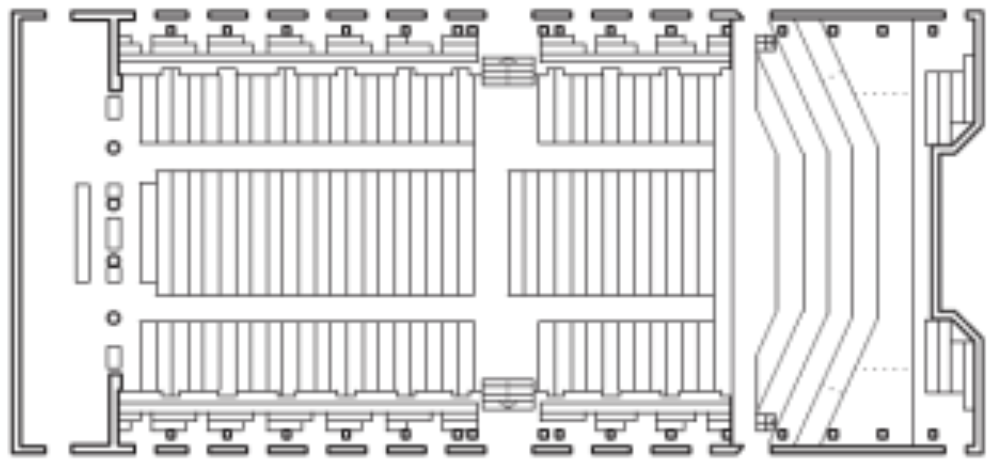
\includegraphics[width=5.4cm]{musikvereinssaal.png}};

\fill[color=deltacolor] (0.8,0) circle[radius=0.08];
\node[color=deltacolor] at (0.8,0) [below] {Quelle};
\draw[->,color=deltacolor,shorten <= 0.2cm]
	(0.8,0) -- +(-0.02,1.6);

\fill[color=echocolor] (4,0) circle[radius=0.08];
\draw[->,color=echocolor,shorten <= 0.2cm]
	(4,0) -- +(2.5,1.6);
\node[color=echocolor] at (4,0) [below] {Mikrofon};

\begin{scope}[xshift=0.3cm,yshift=-3.0cm]
	\def\dy{1}
	\signal
	\draw[->] (-0.1,0) -- (5.3,0) coordinate[label={$t$}];
	\draw[->] (0,-1.1) -- (0,1.3) coordinate[label={right:$f(t)$}];
	\node[color=signalcolor] at (5.3,1.3) [below left] {Signal};
\end{scope}
\begin{scope}[xshift=6.3cm,yshift=-3.0cm]
	\def\dy{15}
	\hall
	\draw[->] (-0.1,0) -- (5.3,0) coordinate[label={$t$}];
	\draw[->] (0,-1.1) -- (0,1.3) coordinate[label={right:$g*f(t)$}];
	\node[color=verhalltcolor] at (5.3,1.3) [below left] {verhalltes Signal};
\end{scope}

\end{tikzpicture}
\end{document}


%\begin{figure}
%\centering
%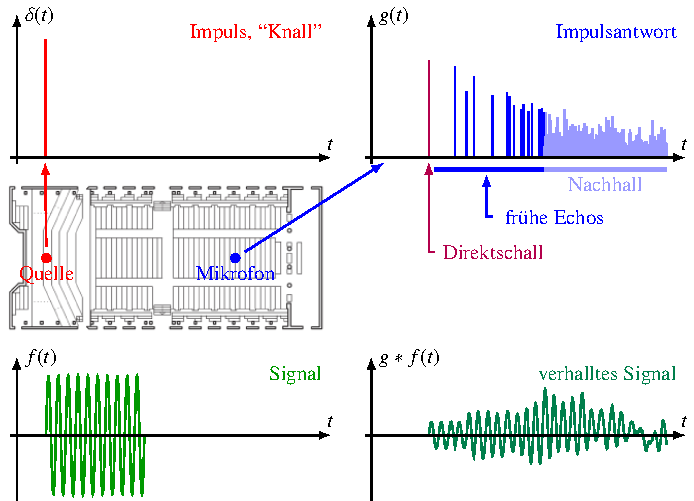
\includegraphics{chapters/030-gruppen/images/konzertsaal.pdf}
%\caption{Echos und Nachhall in einem Konzertsaal.
%Eine einzelner Impuls von einer Quelle (rot) führt beim Mikrofon
%zu einer komplizierten Impulsantwort $g(t)$ bestehend aus
%dem Direktschall, den frühen Echos und dem Nachhall.
%Ein beliebiges Signal $f(t)$ (grün) wird beim Mikrofon als $g*f(t)$
%aufgenommen.
%\label{buch:gruppen:faltung:fig:konzertsaal}}
%\end{figure}
Wie verändern die Reflexionen des Schalls in einem Konzertsaal
den Klang eines Musikinstruments
(Abbildung~\ref{buch:gruppen:faltung:fig:konzertsaal})?
Das Instrument produziert Schallwellen, die sich als Druckschwankungen
$f(t)$ ausbreiten.
Die Wände und Einrichtungsgegenstände reflektieren dies auftreffenden
Schallenwellen in unterschiedlichem Ausmass.
Die Reflexionen treffen beim Zuhörer mit verschiedenen Verzögerungen ein.
Das um $\tau$ verzögerte Signal ist $t\mapsto f(t-\tau)$.
Der Anteil $g(\tau)$ des Signals, des mit Verzögerung $\tau$ beim
Zuhörer eintrifft, heisst die {\em Impulsantwort}.
Das gesamte vom Zuhörer wahrgenommene Signal ist daher die Überlagerung
\begin{equation}
\int_{-\infty}^\infty
g(\tau) 
\,
f(t-\tau)
\,d\tau
\label{buch:gruppen:faltung:eqn:hall}
\end{equation}
all dieser Signale.
Das Integral wird auch als die Faltung $g*f$ bezeichnet.

Die Abbildung photographische mit einem realen Objektiv ist nicht
in der Lage, Punkte beliebig scharf abzubilden.
Stattdessen wird jeder Punkt auf ein Fleck abgebildet, dessen Intensität
mit zunehmender Entfernung vom idealen Bildpunkt abnimmt.
Dafür ist die Wellennatur des Lichts über das Phänomen der Beugung
verantwortlich.
Wir beschreiben das ideal abgebildete Bild als Funktion
$f\colon\mathbb{R}^2\to\mathbb{R}$.
Die Funktion $g(\xi)$ mit $\xi\in\mathbb{R}^2$ beschreibt die
Helligkeit des Flecks, der von einem Punkt erzeugt wird.
Die Helligkeit in einem Punkt $x$ des Bildes setzt sich zusammen
aus der Helligkeit $f(x-\xi)$ in Nachbarpunkten, gewichtet mit
$g(\xi)$, also
\begin{equation}
g*f(x)
=
\int_{\mathbb{R}^2} f(x-\xi)\,g(\xi)\,d\xi.
\label{buch:gruppen:faltung:eqn:pointspread}
\end{equation}
Im Kontext der Bildverarbeitung heisst
die Funktion $g(\xi)$ auch die {\em point spread function}.

%
% Faltung für Funktionen auf einer beliebigen Gruppe
%
\subsection{Faltung für Funktionen auf einer beliebigen Gruppe}
Die Integrale \eqref{buch:gruppen:faltung:eqn:hall} und
\eqref{buch:gruppen:faltung:eqn:pointspread} sind die Faltung
der Fuktionen $f$ und $g$.
Sie verwendet auf wesentliche Art die Gruppenstruktur des
Definitionsbereichs $\mathbb{R}$ der Funktionen.
Die Funktion $f(x-\xi)$ in \eqref{buch:gruppen:faltung:eqn:pointspread}
betrachtet als Funktion von $x$ ist die um $\xi$ verschobene
Funktion $T_\xi f(x)$.

Die obenstehenden Vorbereitungen können als
Ausgangspunkt für die Verallgemeinerung auf eine beliebige Gruppe
in der folgenden Definition verwendet werden.

\begin{definition}[Faltung]
Die Faltung zweier Funktion $f,g\in C(G)$ ist die Funktion
\begin{equation}
(f*g)(x)
=
\int_G f(y)g(y^{-1}x)\,dy.
\label{buch:gruppen:faltung:eqn:deffaltung}
\end{equation}
Im Fall einer additiv geschriebenen, abelschen Gruppe wird die Faltung zu
\begin{equation}
(f*g)(x)
=
\int_G f(y)g(x-y)\,dy.
\label{buch:gruppen:faltung:eqn:deffaltungadditiv}
\end{equation}
\end{definition}

In der Bestrebung, das Integral als Skalarprodukt von Funktionen
zu schreiben, dies muss der Faktor $g(x-y)$ als Funktion von $y$
ausgedrückt werden.

\begin{definition}
Zu einer Funktion $f\colon G\to X$ ist $\check{f}\colon G\to X$ die
Funktion mit den Werten $\check{f}(g) = f(g^{-1})$.
\end{definition}

Mit dieser Definition kann man
\[
T_s f(g)
=
f(s^{-1}g)
=
\check{f}(g^{-1}s)
=
T_g\check{f}(s)
\]
schreiben und damit das Faltungsintegral als
\[
\int_G g(\xi) T_\xi f(x)\,d\xi
=
\int_G g(\xi) T_x \check{f}(\xi)\,d\xi
=
\langle g, T_x\check{f}\rangle
\]
In dieser Form verschwindet das Integral im Skalarprodukt.


%
% Faltung als Produkt
%
\subsection{Faltung als Produkt
\label{buch:gruppen:faltung:subsection:produkt}}
Die Faltung ist ein Produkt, d.~h.~man kann mit Faltungsprodukten 
genau so rechnen, wie man es sich von anderen (nicht kommutativen)
Produkten wie zum Beispiel dem Matrizenprodukt gewöhnt ist.
Dazu müssen zwei Bedingungen erfüllt sein: es müssen das
Assoziativ- und das Distributivgesetz gelten.

%
% Assoziativität
%
\subsubsection{Assoziativität}
Das Assoziativgesetz besagt, dass es in einem Produkt mit mehr als
zwei Faktoren nicht auf die Reihenfolge ankommt, in der man die
Produkte ausführt.
Dies ermöglicht, Faltungsprodukte von drei Funktionen $f$, $g$ und $h$
auch einfach als $f*g*h$ zu schreiben.

\begin{satz}
Die Faltung ist assoziativ, also $(f*g)*h=f*(g*h)$ für Funktionen
$f,g,h\in C(G)$, für die alle Faltungen definiert sind.
\end{satz}

\begin{proof}[Beweis]
Ausgehend von der Definition der Faltung in
\eqref{buch:gruppen:faltung:eqn:deffaltung}
kann man den Wert der zweifachen Faltung als
\begin{align*}
((f*g)*h)(x)
&=
\int_G (f*g)(y) h(y^{-1}x)\,dy
=
\int_G \int_G f(z)g(z^{-1}y) \,dz\, h(y^{-1}x)\,dy
\intertext{berechnen.
Unter der postulierten Voraussetzung, dass alle Integrale existieren,
gilt der Satz von Fubini, der die Reihenfolge der Integrationen zu
vertauschen gestattet.
So wird die Faltung zu
}
&=
\int_G \int_G f(z)g(z^{-1}y) h(y^{-1}x) \,dy \,dz
\\
&=
\int_G f(z) \int_G g(z^{-1}y) h(y^{-1}x) \,dy \,dz
\intertext{Das Integral über $y$ ist invariant unter der Translation
mit $z$, wir schreiben daher $s=z^{-1}y$ und integrieren über $s$
statt $y=zs$:}
&=
\int_G f(z) \int_G g(s) h(s^{-1}z^{-1}x) \,ds \,dz
=
\int_G f(z) (g*h)(z^{-1}x) \,dz
=
(f*(g*h))(x)
\end{align*}
Damit ist die Assoziativität gezeigt.
\end{proof}

%
% Distributivität
%
\subsubsection{Distributivität}
Für ein Produkt wird zusätzlich erwartet, dass man damit rechnen kann
wie mit jedem anderen Produkt.
Dies bedeutet, dass für die Faltung und die Addition von Funktionen
das Distributivgesetz gilt, dass man also Faltungsprodukte
wie gewöhnliche punktweise Produkte von Funktionen
ausmultiplizieren und faktorisieren kann.

\begin{satz}
Für die Faltung und die Addition von Funktionen gilt das Distributivgesetz
\begin{equation}
\begin{aligned}
f*(g+h) &= f*g + f*h
&&\text{und}&
(f+g)*h &= f*h + g*h
\\
(\lambda f) * g &= \lambda (f*g) 
&&&
f*(\lambda f) &= \lambda (f*g).
\end{aligned}
\label{buch:gruppen:faltung:eqn:distributiv}
\end{equation}
\end{satz}

\begin{proof}[Beweis]
Das Distributivgesetz folgt sofort aus der Distributivität der Multiplikation
und der Linearität des Integrals:
\begin{align*}
(f*(g+h))(x)
&=
\int_G f(y) (g+h)(y^{-1}x)\,dy
\\
&=
\int_G f(y) g(y^{-1}x)\,dy
+
\int_G f(y) h(y^{-1}x)\,dy
=
(f*g)(x)
+
(f*h)(x)
\end{align*}
Die anderen Gleichungen \eqref{buch:gruppen:faltung:eqn:distributiv}
folgen auf die gleiche Art.
\end{proof}

%
% Kommutivität
%
\subsubsection{Kommutativität}
Die Faltung von Funktionen auf $\mathbb{R}$ mit der Addition ist
\begin{align*}
(f*g)(x)
&=
\int_{\mathbb{R}} f(y)g(x-y)\,dy
\intertext{mit der Substitution $s=x-y$ wird daraus}
&=
\int_{-\infty}^\infty f(x-s) g(s)\,ds
=
(g*f)(x).
\end{align*}
Das Faltungsprodukt von Funktionen auf $\mathbb{R}$ ist also kommutativ.
Dies gilt jedoch im allgemeinen nicht.

\begin{beispiel}
Die symmetrische Gruppe ist die kleinste nichtabelsche Gruppe.
Es gibt zwei Permutationen $\sigma$ und $\tau$, für die
$\sigma\tau\ne \tau\sigma$ gilt.
Wir berechnen die Faltung der beiden Funktionen 
\[
\raisebox{0.3cm}{$\displaystyle
\delta_\sigma(x) 
=
\begin{cases}
1&\qquad \text{falls $x=\sigma$}\\
0&\qquad \text{sonst}
\end{cases}
\qquad\text{und}\qquad
\delta_\tau(x) 
=
\begin{cases}
1&\qquad \text{falls $x=\tau$}\\
0&\qquad \text{sonst.}
\end{cases}$}
\qedhere
\]
\end{beispiel}

Man kann das auch noch etwas allgemeiner als in diesem Beispiel einer
endlichen Gruppe zeigen.
Dazu sei $G$ eine nichtabelsche Gruppe und $s,t\in G$ seien
zwei verschiedene Elemente, die nicht vertauschen, für die
also $st\ne ts$ ist.
Da die Verknüpfung in der Gruppe stetig ist, gibt es eine kleine
Umgebung $U$ des neutralen Elements derart, dass sich $sU$ und $tU$
nicht schneiden und auch keine gemeinsamen Punkte mit $stU$ und $tsU$, die
sich ebenfalls nicht schneiden.
Falls nicht, kann man die Umgebung $U$ immer noch kleiner machen, um
dies zu erreichen.
Sei ausserdem $f$ eine nichtnegative Funktion, deren Träger in $U$ enthalten
ist.
Wir rechnen jetzt nach, dass die Faltungen $T_sf*T_tf$ und $T_tf*T_sf$ 
nicht gleich sein können, was beweist, dass das Faltungsprodukt
nicht kommutativ sein kann.

Zu diesem Zweck untersuchen wir, wo die Faltung
\begin{equation}
(T_sf * T_tf)(x)
=
\int_G
T_sf(g) 
T_tf(g^{-1}x)
\,dg
=
\int_G
f(s^{-1}g)
f(t^{-1}g^{-1}x)
\,dg
\label{buch:gruppen:faltung:eqn:kommst}
\end{equation}
von $0$ verschieden sein kann.
Der erste Faktor ist höchstens in der Umgebung $sU$ von $0$ verschieden,
der zweite Faktor ist höchstens dann von $0$ verschieden, wenn
$t^{-1}g^{-1}x$ in der Nähe des neutralen Elementes ist.
Da $g$ in der Nähe von $s$ sein muss, ist $t^{-1}g^{-1}$ in der Nähe
von $t^{-1}s^{-1}=(st)^{-1}$.
Der zweite Faktor ist also höchstens dann von $0$ verschieden, wenn
$x$ in der Nähe von $st$ ist.
Der Träger der Faltung ist in einer Umgebung von $st$ enthalten.

Die Gruppenelemente $s$ und $t$ kommen in der Faltung
\eqref{buch:gruppen:faltung:eqn:kommst}
und in der nachfolgenden Diskussion symmetrisch vor.
Daraus folgt, dass die Faltung $T_sf*T_tf$ nur in einer Umgebung von $st$
von $0$ verschieden ist, während $T_tf*T_sf$ nur einer davon disjunkten
Umgebung von $ts\ne st$ von $0$ verschieden ist.
Die beiden Funktionen $T_sf*T_tf$ und $T_tf*T_sf$ können daher
nicht gleich sein, die Faltung ist nicht kommutativ.

%
% Rekonstruktion der Gruppenoperation aus der Faltung
%
\subsubsection{Rekonstruktion der Gruppenoperation aus der Faltung}
Die Diskussion zeigt auch, dass man die Verknüpfung in der Gruppe aus
der Faltung rekonstruieren kann.
Gegeben zwei Elemente $s,t\in G$ und Funktionen $f_n$,
deren Träger in einer Umgebung des neutralen Elementes
enthalten sind, und die für grösser werdendes $n$ schnell kleiner werden..
Dann zeigt die Diskussion oben, dass der Träger der Faltung 
$T_sf_{\varepsilon}*T_tf_{\varepsilon}$ in einer Umgebung von $st$
enthalten sein muss.
Der Träger von $T_sf_n*T_tf_n$ wird kleiner, je grösser man $n$ macht.
Wählt man für jedes $n$ ein Element $g_n$ im Träger der Faltung,
entsteht eine Folge in $G$, die gegen $st$ konvergiert.

Statt die Gruppe und ihre Elemente zu studieren, kann man also die
gleichen Informationen auch aus dem Studium der Faltung von Funktionen
auf der Gruppe gewinnen.
Der Vorteil des Zugangs über Funktionen auf der Gruppe besteht
darin, dass Funktionen einen Vektorraum bilden, auf dem zwei
verschiedene Multiplikationen definiert sind.
Das Skalarprodukt sorgt zusätzlich dafür, dass die quadratintegrierbaren
Funktionen einen Hilbert-Raum bilden.
Diese zusätzlichen algebraischen Strukturelemente geben uns weitere
Werkzeuge in die Hand, die Gruppe zu studieren.








%
% 4-gelfand.tex
%
% (c) 2022 Prof Dr Andreas Müller
%
\section{Charaktere und Gelfand-Transformation
\label{buch:gruppen:section:gelfand}}
\kopfrechts{Charaktere und Gelfand-Transformation}
In diesem Abschnitt suchen wir nach weiteren Möglichkeiten, einen
Zusammenhang zwischen der Algebra der Funktionen auf $G$ mit der Faltung
als Multiplikationsoperation und der Gruppe zu rekonstruieren.

%
% Charaktere der Faltungsalgebra
%
\subsection{Charaktere der Faltungsalgebra}
Die Faltung ist eine ziemlich komplizierte Operation.
Der Vektorraum der Funktionen auf $G$ ist ein unendlichdimensionaler
Vektorraum.
Die Unübersichtlichkeit der Faltung und die Dimension kann etwas
vorborgen werden, indem man komplexwertige Abbildungen untersucht,
die möglichst viel der Struktur erhalten.

\begin{definition}
Ein Vektorraum $A$ heisst {\em Algebra}, wenn aus auf $A$ eine bilineare
und assoziative Multiplikation $A\times A\to A$.
Wenn auf dem Vektorraunm $A$ ausserdem eine Norm definiert ist, dann
heisst $A$ eine normierte Algebra, wenn die Multiplikation die
Ungleichung
\[
\| xy \| \le \|x\|\cdot \|y\|\quad\text{für alle $x,y\in A$}.
\]
\end{definition}

\begin{definition}
Sei $A$ eine normierte Algebra.
Ein Charakter $\chi$ ist eine lineare Abbildung $\chi\colon A\to\mathbb{C}$,
die auch ein stetiger Algebrahomomorphismus ist, d.~h.~es gilt
$\chi(xy)=\chi(x)\chi(y)$.
\end{definition}

Als Beispiel betrachten wir den Vektorraum $C([a,b])$ der stetigen Funktionen
auf dem Intervall $[a,b]$ mit der Supremum Norm.
$C([a,b])$ ist aber auch eine Algebra, da Funktionen punktweise
multipliziert werden können.
Wenn $f,g\in C([a,b])$ zwei stetige Funktionen sind, dann ist
$fg\colon [a,b]\to\mathbb{C}:x\mapsto f(x)g(x)$ ein bilineares und
stetigs Produkt.
Für jeden Punkt $x\in[a,b]$ ist
\[
\chi_x
\colon
C([a,b] \to \mathbb{C}
:
f\mapsto f(x)
\]
eine stetige lineare Abbildung.
Sie ist aber auch ein Algebrahomomorphismus.
Dazu muss man nachrechnen, dass $\chi_x(fg)=\chi_x(f)\chi_y(f)$ ist.
Einsetzen der Definition von $\chi_x$ ergibt
\[
\chi_x(fg)
=
(fg)(x)
=
f(x)g(x)
=
\chi_x(f)\chi_x(g).
\]
Es gibt also zu jedem Punkt des Definitionsbereichs einen Charakter
der Algebra $C([a,b])$.

Man kann zeigen, dass die Homomorphismen von der Form $\chi_x$ 
die einzigen Homomorphismen $A\to\mathbb{C}$ sind.
Dies bedeutet, dass sich der Definitionsbereich der Algebra der
stetigen Funktionen vollständig aus der Algebra rekonstruiert werden 
kann.
Der Unterschied ist aber, dass die $[a,b]$ einfach nur eine Menge ist,
während $C([a,b])$ eine reichhaltige Algebrastruktur hat.

\begin{definition}
\label{buch:gruppen:gelfand:def:spektrum}
Ist $A$ eine Algebra, dann heisst die Menge
\[
\mathrm{X}(A)
=
\operatorname{Hom}(A,\mathbb{C})
\]
der Algebrahomomorphismen von $A$ nach $\mathbb{C}$ heisst das
{\em Spektrum} der Algebra $A$.
\end{definition}

Das Spektrum der Algebra der stetigen Funktionen auf einem Intervall
enthält die Charaktere $\chi_x$ mit $x\in [a,b]$, das Intervall
$[a,b]$ ist eine Teilmenge von $\mathbb{X}(C([a,b]))$.

%
% Homomorphismen G \to C^*
%
\subsection{Homomorphismen $G\to \mathbb{C}^*$}
Sei jetzt $G$ eine Gruppe mit einem Haarschen Mass und der Faltung 
von Funktionen mit kompaktem Träger.
Da die Funktionen alle in $L^2(G)$ drin sind, muss eine lineare
Abbildung nach dem Darstellungssatz von Riesz als ein Skalarprodukt
geschrieben werden können.
Für einen Charakter $\chi\colon L^2(G)\to\mathbb{C}$ muss es also eine
Funktion $\omega\colon G\to\mathbb{C}$ geben derart, dass
\begin{equation}
\langle \omega, f*g\rangle
=
\langle \omega, f\rangle
\langle \omega, g\rangle
\label{buch:gruppen:gelfand:eqn:omegahomo}
\end{equation}
gilt.
Aus dieser Bedingung lässt sich ableiten, dass $\omega$ sehr spezielle
Eigenschaften haben muss.

Seien $s,t\in G$ zwei Elemente der Gruppe.
Sei ausserdem $f$ eine Funktion, die nur in einer kleinen Umgebung 
des neutralen Elementes von $0$ verschieden ist.
Im Skalarprodukt
\[
\langle \omega, T_{s}f\rangle
=
\int_{G} \overline{\omega(x)} f(s^{-1}x) \,dx
\]
ist der Integrand nur für $x$ in unmittelbarer Nähe von $s$ 
$0$ verschieden.
Indem man die Funktion so verändert, dass der Träger kleiner wird,
dann konvergiert das Skalarprodukt gegen den Wert $\omega(s)$.
Aus \eqref{buch:gruppen:gelfand:eqn:omegahomo} folgt dann
\[
\omega(st) = \omega(s)\omega(t).
\]
Die Charaktere der Faltungsalgebra sind also genau die Homomorphismen
$G\mapsto\mathbb{C}^*$ von der Gruppe $G$ in die multiplikative
Gruppe von $\mathbb{C}$.

\begin{beispiel}
Sei $G= \mathbb{R}/2\pi\mathbb{Z}$ die Gruppe der Winkel mit der 
Addition von Winkeln als Gruppenoperation.
Um die Charaktere der Faltungsalgebra der $2\pi$-periodischen Funktionen
zu bestimmen, müssen Homomorphismen $G\to\mathbb{C}$ gefunden werden.
Ist $\omega$ ein solcher Homomorphismus, dann folgt aus
$h=\omega(\frac{2\pi}{n}$, $\omega(2\pi/n)^n = \omega(2\pi)=\omega(0)=1$.
Daher muss $h$ eine komplexe Zahl vom Betrag $1$ sein, die man als
$h=e^{it}$ schreiben kann.
Somit ist $\omega(2\pi k/n) = e^{ikt}$ eine Exponentialfunktion.
Da wir auch gefordert haben, das $\omega$ stetig sein muss folgt,
dass alle Homomorphismen von der Form $x\mapsto e^{ikx}$.
Da $\omega(2\pi)=1$ sein muss, folgt ausserdem, dass $k\in \mathbb{Z}$
ist.
Die Menge der Homomorphismen $G\to\mathbb{R}$ ist daher $\mathbb{Z}$ und
die Menge der Charaktere der Faltungsalgebra ist ebenfalls $\mathbb{Z}$.
\end{beispiel}


%
% Die Gelfand-Transformation
%
\subsection{Die Gelfand-Transformation}
Das Spektrum der Algebra $C([a,b])$ ist das Intervall $[a,b]$,
Es ist also möglich, aus der Algebra mit einer für alle Algebren
durchführbaren Prozedur eine Funktionenalgebra zu machen.
Den Funktionswert $f(x)$  kann man auch als Wert eines 
Algebrahomomorphismus $\chi_x(f) = f(x)$ bekommen.
Dies ist die Motivation für die folgende Definition.

\begin{definition}
Ist $A$ eine Algebra, dann ist die Gelfand-Transformation
die Abbildung
\[
\mathscr{G}
\colon
A \to C(\mathbb{X}(A))
:
a
\mapsto \mathscr{G}a = \hat{a}
\colon \chi \mapsto \hat{a}(\chi) = \chi(a).
\]
\end{definition}

\begin{satz}
Die Gelfand-Transformation ist ein Homomorphismus von Algebren.
\end{satz}

\begin{proof}
Es ist zu zeigen, dass $\mathscr{G}$ linear ist, ein Algebrahomomorphismus
und ausserdem stetig ist.
\begin{itemize}
\item
Linearität:
\begin{align*}
\mathscr{G}(\lambda a+\mu b) (\chi)
&=
\chi( \lambda a + \mu b)
=
\lambda\chi(a) + \mu\chi(b)
=
\lambda(\mathscr{G}a)(\chi)
+
\mu(\mathscr{G}b)(\chi)
\\
\Rightarrow\qquad
\mathscr{G}(\lambda a+ \mu b)
&=
\lambda\mathscr{G}a + \mu\mathscr{G}b.
\end{align*}
Somit ist $\mathscr{G}$ linear.
\item
Algebrahomomorphismus:
\begin{align*}
\mathscr{G}(ab)(\chi)
&=
\chi(ab)
=
\chi(a)\chi(b)
=
(\mathscr{G}a)(\chi)
(\mathscr{G}b)(\chi)
\\
\Rightarrow\qquad
\mathscr{G}(ab)
&=
\mathscr{G}a\cdot \mathscr{G}b.
\end{align*}
\item
\end{itemize}
\end{proof}

Sei jetzt $G$ eine Gruppe und $\mathscr{K}(G)$ die Algebra der
stetige Funktionen mit kompaktem Träger mit der Faltung.
Die Gelfand-Transformation macht aus einer Funktion auf $G$ 
eine Funktion auf dem Spektrum von $\mathscr{K}(G)$.
Ist $\chi\in\mathbb{X}(\mathscr{K}(G))$, dann hat die Gelfandtransformation
von $f\in\mathscr{K}(G)$ den Wert
\[
(\mathscr{G}f)(\chi) = \chi(f).
\]
Da die Gelfand-Transformatioin ein Algebrahomomorophismus ist,
muss  für jeden Homomorphismus $\chi$
\[
\mathscr{G}(f*g)(\chi)
=
(\mathscr{G}f\cdot \mathscr{G}g) (\chi)
=
\mathscr{G}f(\chi)
\mathscr{G}g(\chi)
\]
gelten.
Als Funktion auf $\mathbb{X}(\mathscr{K}(G))$ gilt für die
Gelfand-Transformtion daher
\[
\mathscr{G}(f*g)
=
\mathscr{G}f
\cdot
\mathscr{G}g,
\]
die Gelfand-Transformation macht also aus der Faltung die
gewöhnliche Multiplikation von Funktionen.

Für eine nichtabelsche Gruppe $G$ ist die Faltungsalgebra nicht
kommutativ.
Für zwei Funktionen $f$ und $g$ auf $G$ gilt jetzt aber
\[
\mathscr{G}(f*g)
=
\mathscr{G}f\cdot\mathscr{G}g
=
\mathscr{G}g\cdot\mathscr{G}f
=
\mathscr{G}(g*f).
\]
Die Gelfand-Transformation ignoriert also die Tatsache, dass im allgemeinen
$f * g\ne g*f$ ist.
Eine andere Möglichkeit, dies auszudrücken ist, dass der Kommutator
$f*g-g*f$ im Kern der Gelfand-Transformation liegt, also
\[
\mathscr{G}(f*g-g*f)=0.
\]

Wir wissen auch bereits, dass ein Algebrahomomorphismus
$\chi\colon \mathscr{K}(G)\to\mathbb{C}$ als Skalarprodukt mit
einem Gruppenhomomorphismus 
$\omega\colon G\to\mathbb{C}^*$ geschrieben werden kann.
Die Gelfand-Transformierte hat daher den Wert
\[
(\mathscr{G}f)(\chi)
=
\chi(f)
=
\langle \omega ,f\rangle
=
\int_G \overline{\omega(x)}\,f(x)\,dx.
\]

\begin{beispiel}
Für die Gruppe $\mathbb{R}/2\pi\mathbb{Z}$ der Winkel haben wir die
Menge der Homomorphismen bereits bestimmt, sie ist die Menge der
ganzen Zahlen $k\in\mathbb{Z}$ und der zugehörige Gruppenhomomorphismus
ist $\omega_k(x) = e^{ikx}$.
Die Gelfand-Transformation einer Funktion $f$ ist daher eine Funktion
auf den Zahlen $k\in \mathbb{Z}$ definiert durch
\[
(\mathscr{G}f)(k)
=
\hat{f}(k)
=
\langle \omega_k f\rangle
=
\int_{G/2\pi \mathbb{Z}} \overline{\omega_k(x)}\, f(x) \,dx
=
\int_0^{2\pi} \overline{e^{ikx}} f(x)\,dx
=
\int_0^{2\pi} e^{-ikx} f(x)\,dx.
\]
Die Werte der Fourier-Transformation auf $k\in\mathbb{Z}$ sind bis auf einen
Normierungsfaktor die Fourier-Koeffizienten der Funktion $f$.
\end{beispiel}

Die Gelfand-Transformation ist also eine Verallgemeinerung der
Fourier-Transformation, die automatisch auf eine Art von harmonischer
Analyse von Funktionen auf einer Gruppe führt.
Im Beispiel sind die Funktione $\omega_k$ bezüglich des
Skalarproduktes orthogonal, aber im Allgemeinen wissen wir dies 
noch nicht.
Wir werden in Abschnitt~\ref{buch:gruppen:section:darstellung}
auf diese Frage zurückkommen.



%
% Die duale Gruppe
%
\subsection{Die duale Gruppe}



%
% 5-darstellung.tex -- Darstellungen von Gruppen
%
% (c) 2022 Prof Dr Andreas Müller, OST Ostschweizer Fachhochschule
%
\section{Darstellungen
\label{buch:gruppen:section:darstellung}}
\kopfrechts{Darstellungen}

%
% 6-matrixelemente.tex
%
% (c) 2022 Prof Dr Andreas Müller, OST Ostschweizer Fachhochschule
%
\section{Matrixelemente
\label{buch:gruppen:section:matrixelemente}}
\kopfrechts{Matrixelemente}

%
% 7-charaktere.tex
%
% (c) 2022 Prof Dr Andreas Müller, OST Ostschweizer Fachhochschule
%
\section{Charakter einer Darstellung
\label{buch:gruppen:section:charaktere}}
\kopfrechts{Charakter einer Darstellung}


\section*{Übungsaufgabe}
\rhead{Übungsaufgabe}
\aufgabetoplevel{chapters/030-gruppen/uebungsaufgaben}
\begin{uebungsaufgaben}
\uebungsaufgabe{301}
\uebungsaufgabe{302}
%\uebungsaufgabe{102}
%\uebungsaufgabe{103}
%\uebungsaufgabe{104}
\end{uebungsaufgaben}

